%!TEX TS-program = lualatex
%!TEX encoding = UTF-8 Unicode
%!BIB program = bibtex

\documentclass{mimosis}

\usepackage{metalogo}

%%%%%%%%%%%%%%%%%%%%%%%%%%%%%%%%%%%%%%%%%%%%%%%%%%%%%%%%%%%%%%%%%%%%%%%%
% Some of my favourite personal adjustments
%%%%%%%%%%%%%%%%%%%%%%%%%%%%%%%%%%%%%%%%%%%%%%%%%%%%%%%%%%%%%%%%%%%%%%%%
%
% These are the adjustments that I consider necessary for typesetting
% a nice thesis. However, they are *not* included in the template, as
% I do not want to force you to use them.

% This ensures that I am able to typeset bold font in table while still aligning the numbers
% correctly.
\usepackage{etoolbox}

\usepackage{siunitx}
\DeclareSIUnit\px{px}

\sisetup{%
  detect-all           = true,
  detect-family        = true,
  detect-mode          = true,
  detect-shape         = true,
  detect-weight        = true,
}

%%%%%%%%%%%%%%%%%%%%%%%%%%%%%%%%%%%%%%%%%%%%%%%%%%%%%%%%%%%%%%%%%%%%%%%%
% Hyperlinks & bookmarks
%%%%%%%%%%%%%%%%%%%%%%%%%%%%%%%%%%%%%%%%%%%%%%%%%%%%%%%%%%%%%%%%%%%%%%%%

\usepackage[%
  unicode,
  colorlinks = true,
  citecolor  = RoyalBlue,
  linkcolor  = RoyalBlue,
  urlcolor   = RoyalBlue,
  unicode,
  ]{hyperref}
\hypersetup{
  pdftitle=On Language Modeling and its Applications for Contemporary and Historical French,
  pdfauthor=Pedro Ortiz Suarez
}

\usepackage{bookmark}


%%%%%%%%%%%%%%%%%%%%%%%%%%%%%%%%%%%%%%%%%%%%%%%%%%%%%%%%%%%%%%%%%%%%%%%%
% Fonts
%%%%%%%%%%%%%%%%%%%%%%%%%%%%%%%%%%%%%%%%%%%%%%%%%%%%%%%%%%%%%%%%%%%%%%%%

\ifxetexorluatex
  \setmainfont[Ligatures=TeX]{TeX Gyre Pagella} % Palatino clone
  \linespread{1.05} % a bit more for Palatino
  \RequirePackage{unicode-math}
  \setmathfont{TeX Gyre Pagella Math}
\else
  \usepackage[lf]{ebgaramond}
  \usepackage[oldstyle,scale=0.7]{sourcecodepro}
  \singlespacing
\fi

\usepackage{microtype}

\renewcommand{\th}{\textsuperscript{\textup{th}}\xspace}

\newacronym[description={Principal component analysis}]{PCA}{PCA}{principal component analysis}
\newacronym                                            {SNF}{SNF}{Smith normal form}
\newacronym[description={Topological data analysis}]   {TDA}{TDA}{topological data analysis}

\newglossaryentry{LaTeX}{%
  name        = {\LaTeX},
  description = {A document preparation system},
  sort        = {LaTeX},
}

\newglossaryentry{Real numbers}{%
  name        = {$\real$},
  description = {The set of real numbers},
  sort        = {Real numbers},
}

\makeindex
\makeglossaries

%%%%%%%%%%%%%%%%%%%%%%%%%%%%%%%%%%%%%%%%%%%%%%%%%%%%%%%%%%%%%%%%%%%%%%%%
% Custom Commands and Environments
%%%%%%%%%%%%%%%%%%%%%%%%%%%%%%%%%%%%%%%%%%%%%%%%%%%%%%%%%%%%%%%%%%%%%%%%

%\usepackage{fontawesome}
\usepackage{arydshln}
\usepackage{fontawesome5}
\usepackage{tikz}
\usepackage{tabu}
\usepackage{colortbl}
\definecolor{Gray}{gray}{0.925}
\usetikzlibrary{positioning}

\usepackage{stackengine}
\def\ucr{\scalebox{1}{\stackinset{c}{}{c}{-.1pt}{%
  \textcolor{white}{\sffamily\bfseries\small ?}}{%
  \rotatebox{45}{$\blacksquare$}}}}

\newcommand{\camembert}{CamemBERT\xspace}
\newcommand{\camembertoscar}{CamemBERT\textsubscript{OSCAR}\xspace}
\newcommand{\camembertccnet}{CamemBERT\textsubscript{CCNet}\xspace}
\newcommand{\roberta}{RoBERTa\xspace}
\newcommand{\bert}{BERT\xspace}
\newcommand{\mbert}{mBERT\xspace}
\newcommand{\ccnet}{CCNet\xspace}
\newcommand{\Cabernet}{CaBeRnet\xspace}


\newcolumntype{P}[1]{>{\RaggedRight\hspace{0pt}}p{#1}}

\newcommand{\ELMooscar}{ELMo\textsubscript{OSCAR}\xspace}
\newcommand{\ELMowiki}{ELMo\textsubscript{Wikipedia}\xspace}
\newcommand{\ELMococa}{ELMo\textsubscript{\Cabernet}\xspace}
\newcommand{\ELMocaber}{ELMo\textsubscript{\Cabernet}\xspace}


\newcommand{\ELMocbt}{ELMo\textsubscript{CBT}\xspace}
\newcommand{\ELMocoscar}{ELMo\textsubscript{OSCAR+\Cabernet}\xspace}
\newcommand{\ELMocabercar}{ELMo\textsubscript{OSCAR+\Cabernet}\xspace}

%%%%%%%%%%%%%%%%
\newcommand{\camemberts}{CamemBERTs\xspace}
\newcommand{\camembertwiki}{CamemBERT\textsuperscript{4GB}\hspace{-1.2em}\textsubscript{Wikipedia}\xspace}
\newcommand{\camembertccnetmini}{CamemBERT\textsuperscript{4GB}\hspace{-1.2em}\textsubscript{CCNet}\xspace}
\newcommand{\camembertoscarmini}{CamemBERT\textsuperscript{4GB}\xspace}
%\newcommand{\camembertbase}{CamemBERT\textsubscript{BASE}\xspace}
\newcommand{\camembertccnetlarge}{CamemBERT\textsubscript{LARGE}\xspace}
\newcommand{\camembertlarge}{CamemBERT\textsubscript{LARGE}\xspace}
\newcommand{\camembertccnetlong}{CamemBERT\textsubscript{500k / CCNet}\xspace}
\newcommand{\camembertoscarlong}{CamemBERT\textsuperscript{500k}\hspace{-1.4em}\textsubscript{OSCAR}\xspace}
\newcommand{\camembertoscarswm}{CamemBERT\textsubscript{\it subword}\xspace}
\newcommand{\camembertccnetswm}{CamemBERT\textsubscript{CCNet-{\it subword}}\xspace}
%XLM-R\textsubscript{BASE} \cite{conneau2019xlmr} & 80.1 & 270M \\
\newcommand{\bertbase}{BERT\textsubscript{BASE}\xspace}
\newcommand{\bertlarge}{BERT\textsubscript{LARGE}\xspace}

\newcommand{\lm}[1]{{\color{red}\textbf{LM}: #1}}
\newcommand{\bm}[1]{{\color{blue}\textbf{BM}: #1}}
\newcommand{\po}[1]{{\color{orange}\textbf{PO}: #1}}
\newcommand{\bs}[1]{{\color{PineGreen}\textbf{BS}: #1}}
\newcommand{\ds}[1]{{\color{purple}\textbf{DS}: #1}}

\newcommand{\oscar}{OSCAR\xspace}
\newcommand{\xlmEnFr}{XLM\textsubscript{EN-FR}\xspace}
\newcommand{\xlmmultimlm}{XLM\textsubscript{17-MLM-1280}\xspace}
\newcommand{\xlmmlmtlm}{XLM\textsubscript{MLM-TLM}\xspace}


%%%%%%%%%%%%%%%%%%%%%%%%%%%%%%%%%%%%%%%%%%%%%%%%%%%%%%%%%%%%%%%%%%%%%%%%
% Incipit
%%%%%%%%%%%%%%%%%%%%%%%%%%%%%%%%%%%%%%%%%%%%%%%%%%%%%%%%%%%%%%%%%%%%%%%%

\title{On Language Modeling and its Applications for Contemporary and Historical French}
%\subtitle{A minimal, modern \LaTeX{} package for typesetting your thesis}
\author{Pedro Ortiz Suarez}

\begin{document}

\frontmatter
\selectlanguage{french}

\begin{titlepage}

	\begin{center}
		\begin{minipage}[t]{0.4\textwidth}
			
\includegraphics[height=2cm]{static/media/sorbonne}
		\end{minipage}%
		\hfill
		\begin{minipage}[t]{0.4\textwidth}
			\hfill
			
\includegraphics[height=2cm]{static/media/inria}
		\end{minipage}

		\vspace{0.2cm}
		\LARGE \textsc{Sorbonne Université}\\
		\vspace{0.2cm}
		\normalsize \textsc{Ecole Doctorale Informatique, Télécommunications et Electronique} - ED130\\
		\vspace{0.2cm}
		\textsc{Inria de Paris / Équipe ALMAnaCH}\\

		\vspace{0.4cm}
		\Large \textsc{Thèse de doctorat}\\
		\normalsize Discipline : Informatique\\
		\vspace{0.4cm}
		\normalsize Présentée par \\
		\LARGE \textbf{Pedro \textsc{Ortiz Suarez}}\\
		\vspace{0.4cm}
		\normalsize Dirigée par \\
		\Large \textbf{Laurent \textsc{Romary}} et \textbf{Benoît \textsc{Sagot}}\\
		\vspace{0.4cm}
		\normalsize Pour obtenir le grade universitaire de\\
		\Large \textsc{Docteur} de \textsc{Sorbonne Université}

		\hrulefill\\[0.2cm]

		{\Large  \textbf{A Data-driven Approach to Natural Language Processing\\ for Contemporary and Historical French}}\\[0.1cm]

		\hrulefill\\

		\vspace{0.cm}
		\normalsize Présentée et soutenue publiquement le 27 juin 2022 devant le jury composé de :\\
		\vspace{0.4cm}
		\begin{tabular*}{\linewidth}{@{\extracolsep{\fill}}l c r}
			Francis \textsc{Bach} & Inria - SIERRA & Examinateur \\
			Maud \textsc{Ehrmann} & EPFL & Examinateur \\
			Alexander \textsc{Geyken} & Berlin Academy & Examinateur \\
			Anna \textsc{Korhonen} & University of Cambridge & Rapporteur \\
			Laurent \textsc{Romary} & Inria - ALMAnaCH & Directeur\\
			Benoît \textsc{Sagot} & Inria - ALMAnaCH & Directeur\\
			Holger \textsc{Schwenk} & Facebook AI Research & Rapporteur \\
		\end{tabular*}
	\end{center}

\end{titlepage}

\selectlanguage{english}

\newpage
\null
\thispagestyle{empty}
\newpage

\begin{center}
  \textsc{Abstract}
\end{center}
%
\noindent
%
Scientific documents often use \LaTeX{} for typesetting. While numerous
packages and templates exist, it makes sense to create a new one. Just
because.


\tableofcontents

\mainmatter

%%%%%%%%%%%%%%%%%%%%%%%%%%%%%%%%%%%%%%%%%%%%%%%%%%%%%%%%%%%%%%%%%%%%%%%%
\chapter{Introduction}
%%%%%%%%%%%%%%%%%%%%%%%%%%%%%%%%%%%%%%%%%%%%%%%%%%%%%%%%%%%%%%%%%%%%%%%%

\begin{center}
    \begin{minipage}{0.66\textwidth}
        \begin{small}
            In which the reasons for doing this Ph.D. are laid bare for the whole world to see and we encounter some answers to questions in which, frankly, only an extremely small number of people were interested in the first place.
        \end{small}
    \end{minipage}
    \vspace{0.5cm}
\end{center}

\section{The BASNUM Project}

This thesis is part of the ANR BASNUM project (ANR-18-CE38-0003), which had as its main objective to digitize the \enquote{\emph{Dictionnaire Universel}} (DU) of Antoine Furetière, in its 1701 version reviewed and corrected by Basnage from Beauval \citep{furetiere-1701-dictionnaire}, and to analyze it with digital tools, in order to reveal the importance of this work for the evolution of science and mentalities in the 18\textsuperscript{th} century. The project also aimed to contribute to the current movement to design innovative methods for digitizing, encoding and analyzing texts.

From a purely computational point of view, the BASNUM project intended to carry out two types of tasks:
\begin{enumerate}
    \item a first structuring task where the macrostructure of the dictionary would be annotated,
    \item a second enrichment task which consisted in carrying out a wide range of tasks of information extraction, annotation of the dictionary microstructure and even normalization and modernization of the text.
\end{enumerate}

The first task of automatically structuring dictionaries had been already partially covered by the work of \citet{khemakhem-etal-2017-automatic,khemakhem-etal-2018-enhancing} who developed \emph{GROBID-dictionaries}, a submodule of \emph{GROBID}\footnote{Machine learning library to extract, analyze and restructure raw documents such as PDFs into structured and TEI-encoded documents.} \citep{lopez-etal-2018-grobid} implementing a Java machine learning library for structuring digitized lexical resources in TEI \emph{TEI} format \citep{tei-2018-guidelines}, to enable analysis, extraction and structuring of textual information in such resources. \emph{GROBID-dictionaries} had already obtained promising results and performances \citep{khemakhem-2020-standard}, so much so that it was used to make a first annotation of the \emph{Dictionnaire Universel} macrostructure.

Given the work done by \citet{khemakhem-2020-standard}, we decided to concentrate on the second task of enriching the dictionaries, which at the time remained quite general and abstract, in particular in contrast to the first task of structuring. To approach this task, we had two options: either we develop multiple models and annotation systems dedicated to each of the subtasks involved in this \emph{enrichment} and solely targeting the \emph{Dictionnaire Universel}, or we developed a single generic annotation model capable of addressing all enrichment subtasks and capable of handling not only the \emph{Dictionnaire Universel}, but also other texts and resources from the modern period.\footnote{Between the 16th and 18th century.}

Given the nature of the enrichment task and the fact that new neural language models able to transfer knowledge between different tasks in natural language processing (NLP) had just been published at the beginning of this thesis \cite{peters-etal-2018-deep,devlin-etal-2019-bert}, we decided to focus on the second option and, accordingly, to develop a single general model that we hoped would be able to be used for all these enrichment tasks and for any type of document in Modern or Contemporary French.

By choosing this approach, we also wanted to approach in an indirect way the first task of automatic structuring, this is because we believed that it was possible to improve the first results of \emph{GROBID}-dictionaries by using new neural models. Indeed, \emph{GROBID}-dictionaries relied on CRF models (Conditional Random Fields) \cite{lafferty-etal-2001-conditional} which were widely used for token labeling and classification, but that had been superseded by these neural models in recent years \citep{lample-etal-2016-neural,devlin-etal-2019-bert}. Furthermore, we knew that the developers of \emph{GROBID} had started working with some of these neural models by writing \emph{DeLFT}, a library for text processing, covering token labeling and classification. This library reimplements the latest machine learning models in NLP \citep{lopez-etal-2018-delft} and aims to improve \emph{GROBID}'s pipelines. It is tools and ideas like those contained in \emph{DeLFT} that could be applied to \emph{GROBID}-Dictionaries to significantly improve and expand its capabilities for the benefit of the \emph{BASNUM} project, especially in addition to resources that we had decided to develop.


Having chosen to develop these new models for French, such as \emph{ELMo} \citep{peters-etal-2018-deep} or \emph{BERT} \cite{devlin-etal-2019-bert}, we had to start by building and collecting our own corpus for the pre-training of these architectures, since the contemporary French corpora freely available at the time, such as Wikipedia or frWAC \citep{baroni-etal-2009-the}, were not considered to be large enough for this \citep{liu-etal-2019-roberta}.

Our plan then was to develop a pre-training corpus for Contemporary French, then to pre-train a language model for Contemporary French and finally to use the knowledge transfer capabilities of these architectures to adapt it to Early Modern French, in case we were unable to find enough textual resources to directly pre-train such a language model for Early Modern French. During this thesis, we also wanted to investigate the question of the minimum amount of resources required to successfully pre-train such models, an amount which, at the time, was considered higher than what was available for historical languages \citep{peters-etal-2018-deep,liu-etal-2019-roberta}.

%%%%%%%%%%%%%%%%%%%%%%%%%%%%%%%%%%%%%%%%%%%%%%%%%%%%%%%%%%%%%%%%%%%%%%%%
\section{Transfer Learning in NLP}
%%%%%%%%%%%%%%%%%%%%%%%%%%%%%%%%%%%%%%%%%%%%%%%%%%%%%%%%%%%%%%%%%%%%%%%%

In recent years neural methods for Natural Language Processing (NLP) have consistently and repeatedly improved the state-of-the-art in a wide variety of NLP tasks such as parsing, PoS-tagging, named entity recognition, machine translation, text classification and reading comprehension among others. Probably the main contributing factor in this steady improvement for NLP models is the raise in usage of \emph{transfer learning} techniques in the field. These methods normally consist of taking a pre-trained model and reusing it, with little to no retraining, to solve a different task from the original one it was intended to solve; in other words, one \emph{transfers} the \emph{knowledge} from one task to another.

Most of the transfer learning done in NLP nowadays is done in an unsupervised manner, that is, it normally consists of a  \emph{language model} that is fed unannotated plain text in a particular language; so that it \emph{extracts} or \emph{learns} the basic \emph{features} and patterns of the given language, the model is subsequently used on top of an specialised architecture designed to tackle a particular NLP task. Probably the best known example of this type of model are \emph{word embeddings} which consist of real-valued vector representations that are trained for each word on a given corpus. Some notorious examples of word embeddings are word2vec \citep{mikolov-etal-2013-distributed}, GloVe \citep{pennington-etal-2014-glove} and \mbox{fastText} \citep{mikolov-etal-2018-advances}. All these models are \emph{context-free}, meaning that a given word has one single vector representation that is independent of context, thus for a polysemous word like Washington, one would have one single representation that is reused for the city, the state and the US president.

In order to overcome the problem of polysemy, \emph{contextual} models have recently appeared. Most notably ELMo \citep{peters-etal-2018-deep} which produces deep contextualised word representations out of the internal states of a deep bidirectional language model in order to model word use and how the usage varies across linguistic contexts. ELMo still needs to be used alongside a specialised architecture for each given downstream task, but newer architectures that can be fine-tuned have also appeared. For these, the model is first fed unannotated data, and is then fine-tuned with annotated data to a particular downstream task without relying on any other architecture. some remarkable examples of this type of model are GPT-1, GPT-2 \citep{radford-etal-2018-improving,radford-etal-2019-language}, BERT \citep{devlin-etal-2019-bert} and XLNet \citep{yang-etal-2019-xlnet}; the latter being the current state-of-the-art for multiple downstream tasks. All of these models are different arrangements of the Transformer architecture \citep{vaswani-etal-2017-attention} trained with different datasets, except for XLNet which is an instance of the Transformer-XL \citep{dai-etal-2019-transformer}.

Even though these models have clear advantages, their main drawback is the amount of data that is needed to train them in order to obtain a functional and efficient model. For instance, for the first English version of word2vec, \citet{mikolov-etal-2013-distributed} used a one billion word dataset consisting of various news articles. Later \citet{al-rfou-etal-2013-polyglot} and then \citet{bojanowski-etal-2017-enriching} used the plain text from Wikipedia to train distributions of word2vec and fastText respectively, for languages other than English. Now, the problem of obtaining large quantities of data aggravates even more for contextual models, as they normally need multiple instances of a given word in order to capture all its different uses and in order to avoid overfitting due to the large quantity of hyperparameters that these models have. \citet{peters-etal-2018-deep} for example use a 5.5 billion token\footnote{Punctuation marks are counted as tokens.} dataset comprised of crawled news articles plus the English Wikipedia in order to train ELMo, \citet{devlin-etal-2019-bert} use a 3.3 billion word\footnote{Space sparated tokens.} corpus made by merging the English Wikipedia with the BooksCorpus \citep{zhu-etal-2015-aligning}, and \citet{radford-etal-2019-language} use a 40GB English corpus created by scraping outbound links from Reddit.\footnote{\url{https://www.reddit.com/}}

While Wikipedia is freely available, and multiple pipelines exist\footnote{\url{https://github.com/attardi/wikiextractor}}\textsuperscript{,}\footnote{\url{https://github.com/hghodrati/wikifil}} to extract plain text from it, some of the bigger corpora mentioned above are not made available by the authors either due to copyright issues or probably because of the infrastructure needed to serve and distribute such big corpora. Moreover, the vast majority of both these models and the corpora they are trained with are in English, meaning that the availability of high quality NLP for other languages, specially for low-resource and historical languages, is rather limited.

%% Rephrase

The problem of data is something That we will have to overcome throughout the course of this PhD thesis. In fact rather than concentrating in improving the architectures of these models directly we will focus on developing resources to pre-train them. We will study the impact that balanced corpora and quality has in these models. ...

%%%%%%%%%%%%%%%%%%%%%%%%%%%%%%%%%%%%%%%%%%%%%%%%%%%%%%%%%%%%%%%%%%%%%%%%
\section{Digital Humanities and NLP for Historical Languages}
%%%%%%%%%%%%%%%%%%%%%%%%%%%%%%%%%%%%%%%%%%%%%%%%%%%%%%%%%%%%%%%%%%%%%%%%

With the rise of digital humanities, it is becoming increasingly important to develop high quality tools to automatically process old states of languages. Libraries, archives and museums, among others, are digitizing large numbers of historical sources, from which high quality data must be extracted for further study by specialists of human sciences following new approaches such as ``distant reading'' \cite{moretti-2013-distant}. Many (sub)tasks such as automatic OCR post-correction \cite{rijhwani-etal-2021-lexically} and linguistic annotation \cite{camps-etal-2021-corpus} benefit from pre-trained language models to improve their accuracy.

Languages evolve over time on many levels: from one century to another, we see variations in spelling, syntax, the lexicon etc. However, this variation is not uniform: it tends, at least for ``literate scriptors'' (literature, journalism, law, etc.), to converge towards a single norm over time, and this has especially been the case for French because of the prominent role of the \emph{Académie française} and the \emph{remarqueurs} \cite{ayres-bennett-etal-2011-remarques}. The result of this convergence is, for instance, that spelling and word order within sentences have become stricter, where they were less so in the past. From a computational perspective, historical states of language are therefore not only different from the contemporary state, but, from a computational perspective, are also more complex because they do not follow a strict and explicit norm. In French, this explicit norm  appeared in the 17\textsuperscript{th}~c. and was slowly integrated throughout the 18\textsuperscript{th}~c.

On top of this first linguistic problem, a second issue appears: because the production of textual sources has continued to grow exponentially, it is easier to collect a corpus for contemporary French  than for the 19\textsuperscript{th}\,c. French, which is itself easier than for the 18\textsuperscript{th}\,c. French, etc. The further we go back in time, the more scarce resources are, which creates the following paradox: we have more data when the language is homogeneous and simple for the computer to process, and less when it is heterogeneous and harder to process.

Using contextual word embeddings as input representations has brought clear gains in performances for most of the NLP tasks for which they have been used. However, this has mostly been attested in languages where sufficient (raw) linguistic data is available. For less-resourced languages, the most common approach has been to leverage multilingual models such as mBERT \citep{devlin-etal-2019-bert}

Historical languages are typical cases where available linguistic data is limited, with no chance of acquiring new texts. They are also not normalized by spelling and institutional conventions and tend to be more heterogeneous than contemporary lesser-resourced languages.

\subsection{Medieval French}

Medieval French covers both Old French (9th-13th c.) and Middle French (14th-15th c.). These stages are linguistically close and both precede the adoption of spelling norms. Middle French is more regular than Old French in some respects such as word order \citep{marchello-Nizia-etal-2020-grande} and less in others such as NP structure and pronouns system \citep{marchello-nizia-etal-1979-histoire}. Medieval French covers a set of \textit{Oïl} Romance languages spoken in the kingdom of France between the 9th and the 15th century (\cref{fig:map-dialects}). \footnote{Hand-drawn figure by Mathilde Regnault.} There are around twenty such languages.

Older texts are close to Late Latin, and verse is prevalent until the end of the 13th century. Old French has a relatively free word order. Until the mid-11th century, the prevalent order is \textit{Subject-Object-Verb} (SOV), which is then gradually supplanted by SVO, which is the default order in contemporary French. Unlike most languages with free word order, the functions of verbal arguments are not always given away by morphological clues, the already simplistic case system of Old French disappears progressively through the covered period.

\begin{figure}[thb]
    \centering
    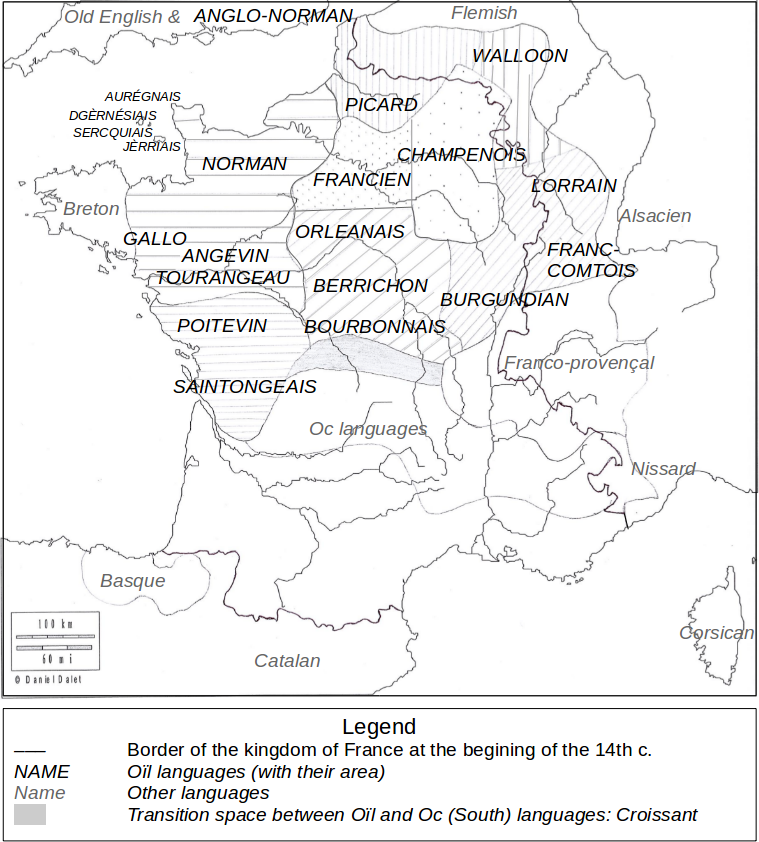
\includegraphics[scale=0.29]{static/media/mod_eval/bertrade/map-dialects2.png}
    \caption{Oïl languages}
    \label{fig:map-dialects}
\end{figure}

There are also many cases of syntactic ambiguity. For example, in the following quote from \emph{Lancelot},\footnote{In the edition from Pierre Kunstmann, from the online \textit{Base de français médiéval}: \url{http://catalog.bfm-corpus.org/CharretteKu}.} (verse ~5436),
both \enquote{la dame} and \enquote{Lancelot} could be the subject or the object of \enquote{Vit} and only the context enables the reader to understand that \enquote{la dame} is the subject.

    \digloss{Dolant et pansif Lancelot Vit la dame}
    {Mournful and meditative Lancelot saw the lady}
    {The lady saw that Lancelot was mournful and meditative.}

Word order is also relatively free within constituents. For example, a noun modifier can be on the left or on the right of its governor, and it is not necessarily preceded by a preposition. In contemporary French, it can only appear on the right, and it is found without a preposition only in some cases like named entities. Because of the general free word order and the absence of punctuation in our treebank, this adds up to the ambiguity of the analysis.

In each of the following examples from the SRCMF corpus, the noun following \emph{roi} (\enquote{king}) has a different analysis: head of \emph{roi}, modifier, argument of the same verb or a different one, with no explicit marking:

\begin{center}
    % beroul. modifieur à gauche.
    \begin{dependency}[theme=simple]
        \begin{deptext}[row 2/.style={font=\small}]
            \textit{Fus} \& \textit{tu} \& \textit{donc} \& \textit{pus} \& \textit{a} \& \textit{la} \& \textbf{\textit{roi}} \& \textit{cort} \\
            %VERB \& PRON \& ADV \& ADV \& ADP \& DET \& NOUN \& NOUN \\
            Were \& you \& then \& no more \& at \& the \& king \& court \\
        \end{deptext}
        \depedge{8}{7}{nmod}
        \depedge[edge start x offset=0.5em]{8}{6}{det}
        \depedge[edge start x offset=1em]{8}{5}{case}
    \end{dependency}

    \raggedright
    \enquote{Then were you not at the king's court anymore?} (\emph{Beroul Tristan})
\end{center}

\begin{center}
    % Graal. modifieur à droite.
    \begin{dependency}[theme=simple]
        \begin{deptext}[row 2/.style={font=\small}]
            \textit{la} \& \textit{fille} \& \textit{au} \& \textit{riche} \& \textbf{\textit{roi}} \& \textit{pescheor} \\
            the \& daughter \& of the \& rich \& king \& fisher \\
        \end{deptext}
        \depedge{5}{6}{flat}
    \end{dependency}

    \raggedright
    \enquote{the daughter of the rich Fisher King} (\emph{Queste del Saint Graal})
\end{center}

\begin{center}
    % Roland. arguments du même verbe.
    \begin{dependency}[theme=simple]
        \begin{deptext}[row 2/.style={font=\small}]
            \textit{De} \& \textit{Guenelun} \& \textit{atent} \& \textit{li} \& \textbf{\textit{reis}} \& \textit{nuveles} \\
            From \& Ganelon \& waits \& the \& king \& news \\
        \end{deptext}
        \depedge{3}{5}{nsubj}
        \depedge[edge start x offset=-0.5em]{3}{6}{obj}
    \end{dependency}

    \raggedright
    \enquote{The king waits for news from Ganelon.} (\emph{Chanson de Roland})
\end{center}

\begin{center}
    % Graal. arguments de verbes différents, et absence de ponctuation.
    \begin{dependency}[theme=simple]
        \begin{deptext}[row 2/.style={font=\small}]
            \textit{Biax} \& \textit{sire} \& \textit{fet} \& \textit{li} \& \textbf{\textit{rois}} \& \textit{escu} \& \textit{vos} \& \textit{envoiera} \& \textit{Diex} \\
            Dear \& Sir \& says \& the \& king \& shield \& you \& send-FUT \& God \\
        \end{deptext}
        \depedge{3}{5}{nsubj}
        \depedge{8}{6}{obj}
    \end{dependency}

    \raggedright
    \enquote{Dear Sir, says the king, God will send you a shield.} (\emph{Queste del Saint Graal})
\end{center}

Furthermore, overt subjects are not mandatory, and are often dropped in texts written in verse until the 12th century, after which the presence of subjects increases through time.
These phenomena are particularly prevalent in verse, where metric and rhyming constraints often lead to more contrived syntactic forms than in prose.

Another source of ambiguity is the variety of spellings, due to the lack of spelling standard. For example, the word \textit{moult} (transl. \textit{a lot (of), very}), emblematic of this period, is initially an adjective, and it is progressively grammaticalized, becoming an adverb. Several forms appear at the same time, some with a declension, some without, and the radical does not have a fixed spelling: \textit{molt(e)(s), molz, mult(e)(s), mul(t)z, mou(l)t}…

\subsection{Early Modern French}\label{def:early}

\begin{table}[!htp]
    \centering\small
    \begin{tabular}{@{}p{0.3\linewidth}p{0.3\linewidth}p{0.3\linewidth}@{}}
        \toprule
        Source                                                                                                                                                                                                                                                                                               & Normalized & Translation \\
        \midrule
        Surquoy, SIRE, s’il plaiſt à voſtre Maieſté de ſe ſouuenir des miſeres de ſon Eſtat, dõt au moins ell’a tiré cét aduantage, qu’en vne grande ieuneſse ell’a acquis vne grande experi\~ece, elle verra que tous les mal-heurs de sõ bas âge ont pris leur commencement en ſemblables occaſions;       &
        \emph{Sur quoi, SIRE, s’il plaît à votre Majesté de se souvenir des misères de son état dont au moins elle a tiré cet avantage, qu’en une grande jeunesse elle a acquis une grande expérience, elle verra que tous les malheurs de son bas âge ont pris leur commencement en semblables occasions~;} &
        \textcolor{gray}{``Whereupon, SIR, if it pleases your Majesty to remember the miseries of her state, from which at least she has derived this advantage, that in great youth she has acquired great experience, she will see that all the misfortunes of her early life took their beginning on similar occasions;''}           \\
        \bottomrule
    \end{tabular}
    \caption{\label{tab:norm_examples}Example of normalization taken from the \emph{Lettres} of \protect\newcite{balzac-1624-lettres}.}
\end{table}

We loosely define Early Modern French as a state of language following Middle French in 1500---following here the \emph{terminus ad quem} used by the \emph{Dictionnaire de Moyen Français} \cite{martin-2020-dictionnaire}---and ending with the French Revolution in 1789. It therefore encompasses three centuries (16\textsuperscript{th}, 17\textsuperscript{th} and 18\textsuperscript{th}\,c.), or two linguistic periods: the \emph{français préclassique} or ``preclassical French'', 1500--1630 and the \emph{français classique} or ``classical French'', 1630--1689; both periodizations are currently used in French linguistics (\emph{e.g.}~by \newcite{vachon-2010-changement} and \newcite{amatuzzi-etal-2019-ameliorer}).

A typical example of Early Modern French, taken from ~\newcite{balzac-1624-lettres}, is given in Table~\ref{tab:norm_examples}. We note here the presence of several phenomena that have now disappeared in contemporary French, such as the presence of abbreviations (\emph{dõt}$\to$\emph{dont}), the long \emph{s} (\emph{ſ}, see\,\emph{miſeres}), the use of \emph{v} instead of \emph{u} (\emph{vne} for \emph{une}), the conservation of etymological letters (\emph{voſtre}$<$Latin~\emph{vŏster} rather than \emph{votre}) and calligraphic letters (\emph{-y} in \emph{Surquoy}), the absence of welding  (\emph{\mbox{mal-heurs}} and not \emph{malheurs}) and the opposite (\emph{Surquoy} and not \emph{Sur quoi}).

For NLP tasks, which process raw sequences, such differences with respect to contemporary French are not trivial, and they prevent the processing of historical texts with tools trained on recent sources.

\section{Outline}



%%%% This is just a draft !!!

\part{Data}
\chapter{OSCAR}
%%%%%%%%%%%%%%%%%%%%%%%%%%%%%%%%%%%%%%%%%%%%%%%%%%%%%%%%%%%%%%%%%%%%%%%%
\chapter{Goclassy}
%%%%%%%%%%%%%%%%%%%%%%%%%%%%%%%%%%%%%%%%%%%%%%%%%%%%%%%%%%%%%%%%%%%%%%%%

\begin{center}
    \begin{minipage}{0.5\textwidth}
        \begin{small}
            In which we present the work of \citep{ortiz-suarez-etal-2019-asynchronous}, introducing the an asynchronous pipeline to Goclassy the first of the OSCAR pipelines, as well as OSCAR 2019 which was the first relase of the OSCAR corpus based on the OSCAR dump of November 2018.
        \end{small}
    \end{minipage}
    \vspace{0.5cm}
\end{center}

%\noindent Common Crawl is a considerably large, heterogeneous multilingual corpus comprised of crawled documents from the internet, surpassing 20TB of data and distributed as a set of more than 50 thousand plain text files where each contains many documents written in a wide variety of languages. Even though each document has a metadata block associated to it, this data lacks any information about the language in which each document is written, making it extremely difficult to use Common Crawl for monolingual applications. We propose a general, highly parallel, multithreaded pipeline to clean and classify Common Crawl by language; we specifically design it so that it runs efficiently on medium to low resource infrastructures where I/O speeds are the main constraint. We develop the pipeline so that it can be easily reapplied to any kind of  heterogeneous corpus and so that it can be parameterised to a wide range of infrastructures. We also distribute a 6.3TB version of Common Crawl, filtered, classified by language, shuffled at line level in order to avoid copyright issues, and ready to be used for NLP applications.

\section{Asynchronous pipeline}

\begin{figure}
    \centering
    \begin{tikzpicture}[auto,scale=0.75, every node/.style={transform shape},font=\sffamily]
        \tikzstyle{nod}=[minimum width=1.65cm,minimum height=6cm,rectangle,rounded corners=10pt,
        fill=red!20, align=center, text width=1.65cm,text centered]
        \tikzstyle{ft} = [minimum width=1.5cm,minimum height=1cm,rectangle,rounded corners=10pt,
        fill=blue!20, align=center, text width=1.5cm,text centered]
        \tikzstyle{fin}=[minimum width=4cm,minimum height=4cm,rectangle,rounded corners=10pt,
        fill=green!20, align=center, text width=4cm,text centered]
        \tikzstyle{arr}=[->,>=stealth,thick]
        \tikzstyle{arr1}=[->,>=stealth,thick, dashed]

        \node[nod] (CC) at (0,0) {Common Crawl};

        \node[minimum width=2cm, text width=2cm,text centered] (TEX1) at (2.5,3.45) {\small Compressed Files};
        \node (GZ1) at (2.5,2.3) {\Huge \faFileArchive[regular]};
        \node (GZ2) at (2.5,1) {\Huge \faFileArchive[regular]};
        \node (GZ3) at (2.5, -0.3) {\Huge \faFileArchive[regular]};
        \node (DGZ) at (2.5, -1.2) {\Huge $\vdots$};
        \node (GZ4) at (2.5,-2.3) {\Huge \faFileArchive[regular]};


        \node[minimum width=1cm, text width=1cm,text centered] (TEX1) at (4.5,3.45) {\small WET Files};
        \node (T1) at (4.5,2.3) {\Huge \faFile*};
        \node (T2) at (4.5,1) {\Huge \faFile*};
        \node (T3) at (4.5, -0.3) {\Huge \faFile*};
        \node (DT) at (4.5, -1.2) {\Huge $\vdots$};
        \node (T4) at (4.5,-2.3) {\Huge \faFile*};

        \node[ft] (F1) at (7,2.3) {fastText};
        \node[ft] (F2) at (7,1) {fastText};
        \node[ft] (F3) at (7,-0.3) {fastText};
        \node (DF) at (7, -1.2) {\Huge $\vdots$};
        \node[ft] (F4) at (7,-2.3) {fastText};

        \node[minimum width=2.3cm, text width=2.3cm,text centered] (TEX1) at (10.25,3.45) {\small Filtered Files Language Tags};
        \node (TA1) at (10.25,2.3) {\Huge \faFile*[regular] $\,$ \faTags};
        \node (TA2) at (10.25,1) {\Huge \faFile*[regular] $\,$ \faTags};
        \node (TA3) at (10.25, -0.3) {\Huge \faFile*[regular] $\,$ \faTags};
        \node (DTA) at (10.25, -1.2) {\Huge $\vdots$};
        \node (TA4) at (10.25,-2.3) {\Huge \faFile*[regular] $\,$ \faTags};


        \node[minimum width=2.3cm, text width=2.3cm,text centered] (TEX1) at (15,3.45) {\small Files Classified by Language};
        \node[fin] (FF) at (15,0) {};
        \node (TF) at (15,1.3) {\Huge \faLanguage $\,\cdots$\faLanguage};
        \node (TF3) at (15, 0) {\Huge \faLanguage $\,\cdots$\faLanguage};
        \node (TF3) at (15, -1.3) {\Huge \faLanguage $\,\cdots$\faLanguage};


        \draw[arr] (1,2.3)--(GZ1);
        \draw[arr] (1,1)--(GZ2);
        \draw[arr] (1,-0.3)--(GZ3);
        \draw[arr] (1,-2.3)--(GZ4);


        \draw[arr] (GZ1)--(T1);
        \draw[arr] (GZ2)--(T2);
        \draw[arr] (GZ3)--(T3);
        \draw[arr] (GZ4)--(T4);


        \draw[arr1] (5,2.5)--(6.1,2.5);
        \draw[arr1] (5,2.3)--(6.1,2.3);
        \draw[arr1] (5,2.1)--(6.1,2.1);

        \draw[arr1] (5,1.2)--(6.1,1.2);
        \draw[arr1] (5,1)--(6.1,1);
        \draw[arr1] (5,0.8)--(6.1,0.8);

        \draw[arr1] (5,-0.1)--(6.1,-0.1);
        \draw[arr1] (5,-0.3)--(6.1,-0.3);
        \draw[arr1] (5,-0.5)--(6.1,-0.5);

        \draw[arr1] (5,-2.1)--(6.1,-2.1);
        \draw[arr1] (5,-2.3)--(6.1,-2.3);
        \draw[arr1] (5,-2.5)--(6.1,-2.5);


        \draw[arr] (8,2.5)--(9.1,2.5);
        \draw[arr] (8,2.3)--(9.1,2.3);
        \draw[arr] (8,2.1)--(9.1,2.1);

        \draw[arr] (8,1.2)--(9.1,1.2);
        \draw[arr] (8,1)--(9.1,1);
        \draw[arr] (8,0.8)--(9.1,0.8);

        \draw[arr] (8,-0.1)--(9.1,-0.1);
        \draw[arr] (8,-0.3)--(9.1,-0.3);
        \draw[arr] (8,-0.5)--(9.1,-0.5);

        \draw[arr] (8,-2.1)--(9.1,-2.1);
        \draw[arr] (8,-2.3)--(9.1,-2.3);
        \draw[arr] (8,-2.5)--(9.1,-2.5);


        \draw[arr] (TA1.0)--(FF);
        \draw[arr] (TA2.0)--(FF);
        \draw[arr] (TA3.0)--(FF);
        \draw[arr] (TA4.0)--(FF);
    \end{tikzpicture}
    \caption{A scheme of the \emph{goclassy} pipeline. The red square represents the Compressed WET files stored on Amazon Web Services. The {\faFileArchive[regular]} icons represent the gzip files stored locally, the {\faFile*} represent one of the 50K WET files. The {\faFile*[regular]} represents the filtered file and the {\faTags} represents a file of language tags, one tag per line in \faFile*[regular]. The {\faLanguage} represents one of the 166 classified files. Each arrow represents an asynchronous non blocking worker and dotted arrows represent a line filtering process.}
    \label{fig:D1}
\end{figure}

We propose a new pipeline derived from the fastText one which we call \texttt{goclassy}, we reuse the fastText linear classifier \citep{joulin-etal-2016-fasttext, joulin-etal-2017-bag} and the pre-trained fastText model for language recognition \citep{grave-etal-2018-learning}, but we completely rewrite and parallelise their pipeline in an asynchronous manner.

The order of operations is more or less the same as in the fastText pre-processing pipeline but instead of clustering multiple operations into a single blocking process, we launch a worker for each operation and we bound the number of possible parallel operations at a given time by the number of available threads instead of the number of CPUs. We implement goclassy using the Go programming language\footnote{\url{https://golang.org/}} so we let the Go runtime\footnote{\url{https://golang.org/src/runtime/mprof.go}} handle the scheduling of the processes. Thus in our pipeline we don't have to wait for a whole WET file to download, decompress and classify in order to start downloading and processing the next one, a new file will start downloading and processing as soon as the scheduler is able to allocate a new process.

When using electromechanical mediums of storage, I/O blocking is one of the main problems one encounters. To overcome this, we introduced buffers in all our I/O operations, a feature that is not present in the fastText pre-processing pipeline. We also create, from the start, a file for each of the 176 languages that the pre-trained fastText language classifier is capable of recognising, and we always leave them open, as we find that getting a file descriptor to each time we want to write, if we wanted leave them open just when needed, introduces a big overhead.

We also do the filtering and cleaning processes at line level before feeding each line to the classifier, which makes us create a new filtered file so that we can have a correspondence with the tag file, which in turn will consume more space, but that will also reduce the amount of unnecessary classifications performed by fastText. The filtered and file tags are then read and lines are appended to its corresponding language file. The writing in the classification step is asynchronous, meaning that process writing a line to the filtered files does not wait for the classifier to write a tag on the tag file. Figure \ref{fig:D1} shows the pipeline up to this point.

After all WET files are processed, we then use Isaac Whitfield's deduplication tool runiq\footnote{\url{https://github.com/whitfin/runiq}} which is based on Yann Collet's xxhash64\footnote{\url{https://github.com/Cyan4973/xxHash}}, an extremely fast non-cryptographic hash algorithm that is resistant to collisions. We finally use the Mark Adler's pigz\footnote{\url{https://zlib.net/pigz/}} for data compression, as opposed to the canonical UNIX tools proposed in the original fastText pipeline. We add both tools to our concurrent pipeline, executing multiple instances of them in parallel, in order to ensure we use the most of our available resources at a given time.

Beyond improving the computational time required to classify this corpus, we propose a simple improvement on the cleaning scheme in the fastText pre-processing pipeline. This improvement allows our pipeline to better take into account the multilingual nature of Common Crawl; that is, we count UTF-8 characters instead of bytes for setting the lower admissible bound for the length of a line to be fed into the classifier. This straightforward modification on the fastText pre-processing pipeline assures we take into account the multiple languages present in Common Crawl that use non-ASCII encoded characters.

Given that our implementation is written in Go, we release binary distributions \footnote{\url{https://github.com/pjox/goclassy}} of goclassy for all major operating systems. Both pigz and runiq are also available for all major operating systems.

\section{Benchmarks}

\begin{table*}[ht!]
    \centering\small
    \resizebox{\linewidth}{!}{
        \begin{tabular}{lrrrcrrrcrrr}\toprule
                     & \multicolumn{3}{c}{10 files} & \phantom{a}             & \multicolumn{3}{c}{100 files} & \phantom{a} & \multicolumn{3}{c}{200 files}                                                                                                                                        \\
            \cmidrule{2-4} \cmidrule{6-8} \cmidrule{10-12}
                     & \multicolumn{1}{c}{Min}      & \multicolumn{1}{c}{Max} & \multicolumn{1}{c}{Mean}      &             & \multicolumn{1}{c}{Min}       & \multicolumn{1}{c}{Max} & \multicolumn{1}{c}{Mean} &  & \multicolumn{1}{c}{Min} & \multicolumn{1}{c}{Max} & \multicolumn{1}{c}{Mean} \\ \midrule
            \emph{real}                                                                                                                                                                                                                                                                            \\
            fastText & 2m50s                        & 6m45s                   & 3m31s                         &             & 13m46s                        & 38m38s                  & 17m39s                   &  & 26m20s                  & 47m48s                  & 31m4s                    \\
            goclassy & 1m23s                        & 3m12s                   & 1m42s                         &             & 7m42s                         & 12m43s                  & 9m8s                     &  & 15m3s                   & 15m47s                  & 15m16s                   \\
            \emph{user}                                                                                                                                                                                                                                                                            \\
            fastText & 26m45s                       & 27m2s                   & 26m53s                        &             & 4h21m                         & 4h24m                   & 4h23m                    &  & 8h42m                   & 8h48m                   & 8h45m                    \\
            goclassy & 10m26s                       & 12m53s                  & 11m0s                         &             & 1h46m                         & 1h54m                   & 1h49m                    &  & 3h37m                   & 3h40m                   & 3h38m                    \\
            \emph{sys}                                                                                                                                                                                                                                                                             \\
            fastText & 40.14s                       & 40.85s                  & 40.56s                        &             & 6m14s                         & 6m17s                   & 6m15s                    &  & 12m26s                  & 12m45s                  & 12m31s                   \\
            goclassy & 37.34s                       & 45.98s                  & 39.67s                        &             & 5m7s                          & 5m34s                   & 5m16s                    &  & 9m57s                   & 10m14s                  & 10m5s                    \\
            \bottomrule
        \end{tabular}
    }
    \caption{Benchmarks are done using the UNIX \texttt{time} tool, are repeated 10 times each and are done for random samples of 10, 100 and 200 WET files. Only the classifying and filtering part are benchmarked. The table shows the minimum, maximum and mean time for the user, real and sys time over the 10 runs. Here ``fastText'' is used as short for the pipeline.}
    \label{tab:Bench}
\end{table*}

We test both pipelines against one another in an infrastructure using traditional electromechanical storage mediums that are connected to the main processing machine via an Ethernet interface, that is, a low I/O speed environment as compared to an infrastructure where one would have an array of SSDs connected directly to the main processing machine via a high speed interface. We use a machine with an Intel\textsuperscript{\textregistered} Xeon\textsuperscript{\textregistered} Processor E5-2650 2.00 GHz, 20M Cache, and 203.1 GiB of RAM. We make sure that no other processes apart from the benchmark and the Linux system processes are run. We do not include downloading, decompression or deduplication in our benchmarks as downloading takes far too much time, and deduplication and compression were performed with third party tools that don't make part of our main contribution. We are mainly interested in seeing how the way the data is fed to the classifier impacts the overall processing time.

Benchmarks in table \ref{tab:Bench} of our goclassy pipeline show a drastic reduction in processing time compared to the original fastText prepossessing pipeline. We show that in our particular infrastructure, we are capable of reducing the \emph{real} time as measured by the \texttt{time} UNIX tool almost always by half. The \emph{user} time which represents the amount of CPU time spent in user-mode code (outside the kernel) within the process is almost three times lower for our goclassy pipeline, this particular benchmark strongly suggest a substantial reduction in energy consumption of goclassy with respect to the fastText pipeline.

As we understand that even an infrastructure with more than 20TB of free space in traditional electromechanical storage is not available to everyone and we propose a simple parametrization in our pipeline that actively deletes already processed data and that only downloads and decompresses files when needed, thus ensuring that no more than 10TB of storage are used at a given time. We nevertheless note that delaying decompression increases the amount of computation time, which is a trade-off that some users might make as it might be more suitable for their available infrastructure.

\section{OSCAR}

Finally, we are aware that some users might not even have access to a big enough infrastructure to run our pipelines or just to store all the Common Crawl data. Moreover, even if previously used and cited in NLP and Machine Learning research, we note that there is currently no public distribution of Common Crawl that is filtered, classified by language and ready to use for Machine Learning or NLP applications. Thus we decide to publish a pre-processed version of the November 2018 copy of Common Crawl which is comprised of usable data in 166 different languages, we publish\footnote{\url{https://team.inria.fr/almanach/oscar/}} our version under the name OSCAR which is short for \emph{Open Super-large Crawled ALMAnaCH\footnote{\url{https://team.inria.fr/almanach/}} coRpus}.

After processing all the data with goclassy, the size of the whole Common Crawl corpus is reduced to 6.3TB, but in spite of this considerable reduction, OSCAR still dwarfs all previous mentioned corpora having more 800 billion ``words'' or spaced separated tokens and noting that this in fact is an understatement of how big OSCAR is, as some of the largest languages within OSCAR such as Chinese and Japanese do not use spaces. The sizes in bytes for both the original and the deduplicated versions of OSCAR can be found in table \ref{tab:langs-goclassy}. OSCAR is published under the \emph{Creative Commons CC0 license (``no rights reserved'')}\footnote{\url{http://creativecommons.org/publicdomain/zero/1.0/}}, so it is free to use for all applications.

\section{Conclusions}

We are sure that our work will greatly benefit researchers working on an either constrain infrastructure or a low budget setting. We are also confident, that by publishing a classified version of Common Crawl, we will substantially increase the amount of available public data for medium to low resource languages, thus improving and facilitating NLP research for them. Furthermore, as our pipeline speeds-up and simplifies the treatment of Common Crawl, we believe that our contribution can be further parallelised and adapted to treat multiple snapshots of Common Crawl opening the door to what would be otherwise costly diachronic studies of the use of a given language throughout the internet.

Finally, we note that both our proposed pipeline is data independent, which means that they can be reused to process, clean and classify any sort of big multilingual corpus that is available in plain text form and that is UTF-8 encoded; meaning that the impact of our work goes way beyond a single corpus.
\section{Introduction}
Access to multilingual datasets for NLP research has vastly improved over the past years. A variety of web-derived collections for hundreds of languages is available for anyone to download, such as ParaCrawl~\citep{espla-etal-2019-paracrawl, banon-etal-2020-paracrawl}, WikiMatrix~\citep{schwenk-etal-2021-wikimatrix} CCAligned~\citep{el-kishky-etal-2020-ccaligned}, \mbox{OSCAR}~\citep{ortiz-suarez-etal-2019-asynchronous, ortiz-suarez-etal-2020-monolingual}, and several others.
%though ma \citep{joshi-etal-2020-state}.
These have in turn enabled a variety of highly multilingual models, like mT5 \citep{xue-etal-2021-mt5}, M2M\nobreakdash-100 \citep{fan-etal-2020-beyond}, M4 \citep{arivazhagan-etal-2019-massively}.
% Recent approaches that employ large-scale multilingual systems have shown potential for some generalization across typologically different languages \cite{pires-etal-2019-multilingual,papadimitriou-etal-2021-deep}. .

Curating such datasets relies on the websites giving clues about the language of their contents (e.g. a language identifier in the URL) and on automatic language classification (LangID).
%and filtering tools, and a range of evaluation sets and metrics to compile high-quality datasets. 
It is commonly known that these automatically crawled and filtered datasets tend to have overall lower quality than hand-curated collections~\citep{koehn-etal-2020-findings}, but their quality is rarely measured directly, and is rather judged through the improvements they bring to downstream applications~\citep{schwenk-etal-2021-wikimatrix}.

Building NLP technologies with automatically crawled datasets is promising. This is especially true for low-resource languages, because data scarcity is one of the major bottlenecks for deep learning approaches.
However, there is a problem: There exists very little research on evaluating both data collections and automatic crawling and filtering tools for low-resource languages.
As a result, although many low-resource languages are covered by the latest multilingual crawl data releases, their quality and thus usability is unknown. %Inferring the quality from higher-resource, well-evaluated and studied subsets of the same crawls would be rather naive, since errors can accumulate easily in the pipeline of multilingual web mining.

%ideas for start:
%\begin{itemize}
%    \item ``How good is my data?'' -- data quality becomes more and more of a concern with scaling up: giant models feeding on giant collections of (multimodal) data collections, facilitated by the easy access to data on the web. 
%    \item work we could cite:
%    \item On paper/in theory/in principle/according to raw data statistics, the situation for low-resource languages should have improved over the past year, with large multilingual data collections being released publicly. (insert example) The prospects for building NLP technologies on the base of these collections seem promising, since data sparsity is one of the bottlenecks for the application of current deep learning approaches. However, ...
%\end{itemize}
%While companies frequently use in-house curated data sets, these data sets are used frequently for academic research and publications, so it was important to understand them better.
To shed light on the quality of data crawls for the lowest resource languages, we perform a manual data audit for 230 per-language subsets of five major crawled multilingual datasets: CCAligned~\citep{el-kishky-etal-2020-ccaligned}, ParaCrawl~\citep{espla-etal-2019-paracrawl,banon-etal-2020-paracrawl}, WikiMatrix~\citep{schwenk-etal-2021-wikimatrix}, OSCAR~\citep{ortiz-suarez-etal-2019-asynchronous, ortiz-suarez-etal-2020-monolingual} and mC4~\citep{xue-etal-2021-mt5}. We propose solutions for effective, low-effort data auditing (section~\ref{sec:audit}), including an error taxonomy. Our quantitative analysis reveals surprisingly low amounts of valid in-language data, and identifies systematic issues across datasets and languages. In addition, we find that a large number of datasets is labeled with nontransparent or incorrect language codes (section~\ref{sec:codes}). This leads us to reflect on the potential harm of low-quality data releases for low-resource languages (section~\ref{sec:risk}), and provide a set of recommendations for future multilingual data releases (section~\ref{sec:recommendation}).

% The contributions of this paper are as follow:
% \begin{itemize}
%   \item We provide quantitative quality evaluations for 124 languages in five public datasets
%   \item We demonstrate that native-speaker expertise is not necessary to XXX 
%     \item the comparison across languages and corpora lets us identify the main pain points for future work 
%       \item reflection on the harm of low-quality data releases for low-resource languages (Section~\ref{sec:risk})
% \end{itemize}

\begin{table*}[th]
    \centering
    \resizebox{\textwidth}{!}{%
        \begin{tabular}{lccccc}
            \toprule
                            & \multicolumn{3}{c}{\textbf{Parallel}} & \multicolumn{2}{c}{\textbf{Monolingual}}                                                       \\
            \cmidrule(lr){2-4} \cmidrule(lr){5-6}
                            & \textbf{CCAligned}                    & \textbf{ParaCrawl v7.1}                  & \textbf{WikiMatrix} & \textbf{OSCAR} & \textbf{mC4} \\
            \midrule
            \#languages     & 137                                   & 41                                       & 85                  & 166            & 101          \\
            Source          & CC 2013--2020                         & selected websites                        & Wikipedia           & CC 11/2018     & CC all       \\
            Filtering level & document                              & sentence                                 & sentence            & document       & document     \\
            Langid          & FastText                              & CLD2                                     & FastText            & FastText       & CLD3         \\
            Alignment       & LASER                                 & Vec/Hun/BLEU-Align                       & LASER               & -              & -            \\
            Evaluation      & TED-6                                 & WMT-5                                    & TED-45              & POS/DEP-5      & XTREME       \\
            \bottomrule
        \end{tabular}%
    }
    \caption{Comparison of parallel and monolingual corpora extracted from web documents, including their downstream evaluation tasks. All parallel corpora are evaluated through machine translation evaluation with BLEU. TED-6: \texttt{da}, \texttt{cr}, \texttt{sl}, \texttt{sk}, \texttt{lt}, \texttt{et}; TED-45: 45-language subset of ~\citep{qi-etal-2018-pre}; WMT-5: \texttt{cs}, \texttt{de}, \texttt{fi}, \texttt{lv}, \texttt{ro}. POS/DEP-5: part-of-speech labeling and dependency parsing for \texttt{bg}, \texttt{ca}, \texttt{da}, \texttt{fi}, \texttt{id}.}
    \label{tab:corpora}
\end{table*}
% CC: CommonCrawl; TED-6: da, cr, sl, sk, lt, et; TED-50: TODO cite Qi et al. 2018; WMT-5: cs, de, fi, lv, ro.
%fastText: 176 languages, Wikipedia & Tatoeba

\section{Related Work}\label{sec:related}

Corpora collected by web crawlers are known to be noisy~\citep{junczys-dowmunt-2019-microsoft}. In highly multilingual settings, past work found that web-crawls of lower-resource languages have serious issues, especially with segment-level LangID~\citep{caswell-etal-2020-language}.
%Repeated studies have shown that 
Cleaning and filtering web-crawls can boost general language modeling~\citep{gao-etal-2020-the,brown-etal-2020-language,raffel-etal-2020-exploring} and downstream task performance~\citep{moore-lewis-2010-intelligent,xu-koehn-2017-zipporah,khayrallah-koehn-2018-impact,brown-etal-2020-language}.

% zaricna2015word
As the scale of ML research grows, it becomes increasingly difficult to validate automatically collected and curated datasets \citep{biderman-etal-2020-pitfalls,prabhu2020large,bender2021dangers}.
%Data Quality Considerations for Big Data and Machine Learning: Going Beyond Data Cleaning and Transformations \citep{gudivada2017data}
Several works have focused on advancing methodologies and best practices to address these challenges. \citet{bender2018data} introduced data statements, a documentary framework for NLP datasets that seeks to provide a universal minimum bar for dataset description. Similar work has focused on
% been done on systematizing documentation in other areas in data science and machine learning, including work focusing on 
online news \citep{kevin-etal-2018-information}, data ethics \citep{sun2019mithralabel}, and data exploration \citep{holland2018dataset}, as well as generalist work such as \citep{gebru2018datasheets}. There is a large literature on filtering text data for various NLP tasks, e.g. \cite{axelrod-etal-2011-domain,moore-lewis-2010-intelligent,wang2018denoising,kamholz-etal-2014-panlex,junczys-dowmunt-2018-dual,caswell-etal-2020-language}.

Closest to our work is the analysis of a highly multilingual (non-publicly available) web-crawl and LangID related quality issues by \citet{caswell-etal-2020-language}.
%, performing a highly multilingual web-crawl and then systematically analyzing the LangID related quality issues. 
%However, though 
They perform a brief analysis of the quality of OSCAR
%, but omit analyses of any other public datasets, 
with the focus only on the presence of in-language content.

% Previous work also focused on automatic methods to improve data quality for both monolingual and parallel corpora.  proposes a method for filtering noisy parallel data based on cross-entropy scores of two inverse translation models which shows significant improvement over baselines models.  demonstrate that the language identification models for low-resource languages are almost unusable despite the belief that the task is ``solved". Authors propose two filtering techniques to alleviate common problems these models fall prey to. TODO: Jim: Just wrote this out fully as a reference. Might need to shorten it later.

% Diversity
% The availability of data resources has shaped research in NLP; most systems are trained and evaluated on a few dominant language families. On the other hand, resource-scarce languages have only recently started to receive attention with focused communities working on these languages \citep{joshi-etal-2020-state}. Recent approaches that employ large-scale multilingual systems have shown potential for some generalization across typologically different languages, relying only on an unlabeled monolingual datasets \cite{pires-etal-2019-multilingual,papadimitriou-etal-2021-deep}. 
% 

% TODO: Summarize the following related works into coherent paragraphs.
% \paragraph{Corpus cleaning}
% \begin{itemize}
% % \item Dual Conditional Cross-Entropy Filtering of Noisy Parallel Corpora \citep{junczys-dowmunt-2018-dual} (covered)
% % \item Language ID in the Wild: Unexpected Challenges on the Path to a Thousand-Language Web Text Corpus. \citep{caswell-etal-2020-language} (covered)
% \item Garbage in Garbage Out \citet{geiger2020garbage} (this wasn't really about corpus cleaning. not sure how to include it)
% \end{itemize}

% \paragraph{Reports about data noise}
% \begin{itemize}
%     \item Language ID in the Wild: Unexpected Challenges on the Path to a Thousand-Language Web Text Corpus  \citep{}
%     \item Comparing parallel corpora and evaluating their quality \citep{kaalep2007comparing} (this is not included yet but the scope if smaller than others)
% \end{itemize}

%NLP data quality evaluation

% \paragraph{Diversity / low-resource language representation in NLP}
% \begin{itemize}
%     % \item The State and Fate of Linguistic Diversity and Inclusion in the NLP World \citep{joshi-etal-2020-state}
%     % \item How Multilingual is Multilingual BERT? \citep{pires-etal-2019-multilingual} 
%     \item Findings of the WMT 2019 Shared Task on Parallel Corpus Filtering for Low-Resource Conditions \citep{koehn-etal-2019-findings}
% \end{itemize}

% \paragraph{Nutrition Labels \& datasheets}
% \begin{itemize}
%     \item Datasheets for Datasets 
%     \item The Dataset Nutrition Label: A Framework To Drive Higher Data Quality Standards \cite{holland2018dataset}
% \end{itemize}


\section{Multilingual Corpora}\label{sec:crawls}
Table \ref{tab:corpora} provides an overview of the corpora of interest in this work. We selected the corpora for their multilinguality and the inclusion of understudied languages in NLP. With the exception of WikiMatrix and Paracrawl, all corpora are derived from CommonCrawl (CC).\footnote{\url{http://commoncrawl.org/}} %s, and distinguish themselves by the choice of filtering methods, LangID and automatic alignment technology.
%LangID is crucial to corpus creation, since any issues within might propagate, e.g. bias recognizing document types similar to what it was trained on, or errors in language identifiers.\footnote{\url{https://github.com/facebookresearch/fastText/issues/482}}



%TODO briefly describe recipe for web-mining data like in https://arxiv.org/pdf/2010.14571.pdf in Appendix K 
%Describe pipeline to get to a crawled corpus for a language or at least which components play a role, so that we can later refer to them and partially explain the type of garbage that ends up there and point out the bottlenecks (lang id!!!!) for anyone out there looking for research projects. (Note: https://arxiv.org/pdf/2010.14571.pdf in Appendix K gives a recipe for web-mining data)

%TODO: briefly mention what each dataset has been used for

\paragraph{CCAligned~\citep{el-kishky-etal-2020-ccaligned}}is a %119-language\footnote{119 of originally 137 available for download (02/2021)}
%Although 137 language pairs are reported in ~\citet{el-kishky-etal-2020-ccaligned}, only 119 sentence-level corpora were available to download on \url{statmt.org} as of February 2021.}
parallel dataset built off 68 CC snapshots. Documents are aligned if they are in the same language according to FastText LangID~\citep{joulin-etal-2016-fasttext,joulin-etal-2017-bag}, and have the same URL but for a differing language code. These alignments are refined with cross-lingual LASER embeddings \citep{artetxe-schwenk-2019-massively}. For sentence-level data, they split on newlines and align with LASER, but perform no further filtering.
Human annotators evaluated the quality of document alignments for six languages (\texttt{de}, \texttt{zh}, \texttt{ar}, \texttt{ro}, \texttt{et}, \texttt{my}) selected for their different scripts and amount of retrieved documents, reporting precision of over 90\%.
% Latin, Chinese, Arabic, Burmese script
The quality of the extracted parallel sentences was evaluated in a machine translation (MT) task on six European (\texttt{da}, \texttt{cr}, \texttt{sl}, \texttt{sk}, \texttt{lt}, \texttt{et}) languages of the TED corpus~\citep{qi-etal-2018-pre}, where it compared favorably to systems built on crawled sentences from WikiMatrix and ParaCrawl v6. %, yielding BLEU scores in a range between 15 and 38.  

\paragraph{Multilingual C4 (mC4)~\citep{xue-etal-2021-mt5}} is a document-level dataset used for training the mT5 language model. It consists of monolingual text in 101 languages and is generated from 71 CC snapshots. It filters out pages that contain less than three lines of at least 200 characters and pages that contain bad words~\citep{emerick2018list}. Since this is a document-level dataset, we split it by sentence and deduplicate it before rating. For language identification, it uses CLD3~\citep{botha-etal-2017-natural}, a small feed-forward neural network that was trained to detect 107 languages.
% \footnote{\url{https://github.com/LDNOOBW/}}
% \footnote{\url{https://github.com/google/cld3/}}
The mT5 language model pre-trained on mC4
%\footnote{Upsampling lower-resource languages.} 
is evaluated on 6 tasks of the XTREME benchmark~\citep{hu2020xtreme} covering a variety of languages and outperforms other multilingual pre-trained language models such as mBERT~\citep{devlin-etal-2019-bert} and XLM\nobreakdash-R~\citep{conneau-etal-2020-unsupervised}.%\footnote{mBERT is trained on Wikipedia, {XML\nobreakdash-R} on CommonCrawl.} 

\paragraph{OSCAR~\citep{ortiz-suarez-etal-2019-asynchronous, ortiz-suarez-etal-2020-monolingual}}is a set of monolingual corpora extracted from CC snapshots, specifically from the plain text \emph{WET} format distributed by CC which removes all the HTML tags and converts the text formatting to UTF-8. It is deduplicated and follows the same approach as~\citet{grave-etal-2018-learning} by using FastText LangID
%~\citep{joulin-etal-2016-fasttext, joulin-etal-2017-bag} 
on a line-level.
%No other filtering was applied.
% \footnote{\url{https://fasttext.cc/docs/en/language-identification.html}
For five languages (\texttt{bg}, \texttt{ca}, \texttt{da}, \texttt{fi}, \texttt{id}) OSCAR corpora were used to train ELMo~\citep{peters-etal-2018-deep} embeddings for POS tagging and dependency parsing, outperforming those trained on Wikipedia~\citep{ortiz-suarez-etal-2020-monolingual}. % -sourced embeddings


\paragraph{ParaCrawl v7.1} is a parallel dataset with 41 language pairs primarily aligned with English (39 out of 41) and mined using the parallel-data-crawling tool Bitextor \citep{espla-etal-2019-paracrawl,banon-etal-2020-paracrawl} which includes downloading documents, preprocessing and normalization, aligning documents and segments, and filtering noisy data via Bicleaner.
% \footnote{\url{https://github.com/bitextor/bicleaner}}
ParaCrawl focuses on European languages, but also includes 9 lower-resource, non-European language pairs in v7.1.
% TODO: https://www.aclweb.org/anthology/2020.eamt-1.31.pdf \citep{ramirez-sanchez-etal-2020-bifixer}
Sentence alignment and sentence pair filtering choices were optimized for five languages (\texttt{mt}, \texttt{et}, \texttt{hu}, \texttt{cs}, \texttt{de}) by training and evaluating MT models on the resulting parallel sentences. An earlier version, ParaCrawl v5, was shown to improve translation quality on WMT benchmarks for~\texttt{cs}, \texttt{de}, \texttt{fi}, \texttt{lv}, \texttt{ro}.


\paragraph{WikiMatrix~\citep{schwenk-etal-2021-wikimatrix}}is a public dataset containing 135M parallel sentences in 1620 language pairs (85 languages) mined from Wikipedia. Out of the 135M parallel sentences, 34M are aligned with English.
%which relies on first learning multilingual sentence embeddings, and then applying the cosine distance metric to determine whether two sentences are close enough to be considered translations of each other.
The text is extracted from Wikipedia pages, split into sentences, and duplicate sentences are removed. FastText LangID is used before identifying bitext with LASER's distance-based mining approach.
The margin threshold is optimized by training and evaluating downstream MT models on four WMT benchmarks (\texttt{de-en}, \texttt{de-fr}, \texttt{cs-de}, \texttt{cs-fr}). The final dataset is evaluated through TED translation models between 45 languages, with highest quality for translations between English and e.g. \texttt{pt}, \texttt{es}, \texttt{da}, and lowest for \texttt{sr}, \texttt{ja}, \texttt{mr}, \texttt{zh\_TW}.
%In the audit 
We focus on language pairs with English on one side.
% https://github.com/facebookresearch/LASER/blob/master/tasks/WikiMatrix/WikiMatrix-bleu.pdf
%TODO used for example in https://arxiv.org/abs/2010.11125
%TODO used in https://www.aclweb.org/anthology/2020.emnlp-main.121.pdf 

%\paragraph{FastText LangID}
%The FastText~\citep{grave-etal-2018-learning} language classifier was trained on Wikipedia, Tatoeba, SETimes,\footnote{\url{https://fasttext.cc/docs/en/language-identification.html}} so any issues within these collections might propagate, and there might be a bias recognizing similar document types, e.g. lexicon entries, in CC. 176 languages



\section{Auditing Data Quality}\label{sec:audit}
None of the above datasets has been evaluated for quality on the sentence level (exception: several languages in ParaCrawl v3), and downstream evaluations are centered around a small fraction of higher-resource languages. This is insufficient for drawing conclusions about the quality of individual or aligned sentences, and about the entirety of languages. %but only on document/URL level and a small selection of downstream tasks. 
%: Samples of URLs or retrieved documents were evaluated for their accuracy, and derived Machine Translation (MT) and NLP systems are shown to perform well for a subset of language pairs. 
%This does not guarantee that individual or aligned sentences extracted from those documents or URLs are of high quality, nor is the subset of languages sufficient to guarantee for the data quality of the whole corpus. %(TODO stats).
% Additionally: publication bias: negative results might not have been published (are harder to publish)
%excuse: no speaker available, reality: speaker not necessarily needed
To close this gap, we conduct a data quality audit that focuses on the lowest-resource and most under-evaluated languages, but also covers mid- and high-resource languages for comparison. %; and (2) aims at width rather than depth in order to draw comparisons across datasets and languages.


\begin{table*}[th]
    \small
    \centering
    \begin{tabular}{|ll|}
        \hline
        \hline
        \multicolumn{2}{|c|}{\textbf{Correct Codes}}                                                                                \\
        \hline
        \multicolumn{2}{|l|}{\textbf{\texttt{CC}:} \textit{Correct translation, natural sentence}}                                  \\
        \hdashline
        \texttt{en} The Constitution of South Africa            & \texttt{nso} Molaotheo wa Rephabliki ya Afrika Borwa              \\
        \texttt{en} Transforming your swimming pool into a pond & \texttt{de} Umbau Ihres Swimmingpools zum Teich                   \\
        \hline
        \multicolumn{2}{|l|}{\textbf{\texttt{CB}:} \textit{Correct translation, Boilerplate or low quality}}                        \\
        \hdashline
        \texttt{en} Reference number: 13634                     & \texttt{ln} Motango ya référence: 13634                           \\
        \texttt{en} Latest Smell Stop Articles                  & \texttt{fil} Pinakabagong mga Artikulo Smell Stop                 \\
        %  \texttt{en} Weight (Male): 8,6 - 13,5 kg & \texttt{ts} Ntiko (Xinuna): 8, 6 - 13, 5 kg \\
        \hline
        \multicolumn{2}{|l|}{\textbf{\texttt{CS}:} \textit{Correct translation, Short}}                                             \\
        \hdashline
        \texttt{en} movies, dad                                 & \texttt{it} cinema, pap\`{a}                                      \\
        \texttt{en} Halloween - without me                      & \texttt{ay} Hallowen – janiw nayampejj                            \\
        \hline
        \hline
        \multicolumn{2}{|c|}{\textbf{Error Codes}}                                                                                  \\
        \hline
        \multicolumn{2}{|l|}{\textbf{X:} \textit{Incorrect translation, but both correct languages}}                                \\
        \hdashline
        \texttt{en} A map of the arrondissements of Paris       & \texttt{kg} Paris kele mbanza ya kimfumu ya Fwalansa.             \\
        \texttt{en} Ask a question                              & \texttt{tr} Soru sor Kullanıma g{\"o}re se\c{c}im                 \\
        \hline
        \multicolumn{2}{|l|}{\textbf{\texttt{WL}:} \textit{Source OR target wrong language, but both still linguistic content}}     \\
        \hdashline
        \texttt{en} The ISO3 language code is zho               & \texttt{zza} T{\' a}im eadra bracach mar bhionns na frogannaidhe. \\
        %  \texttt{en} sicilianu: Johannesburg & \texttt{ve} Tshivenda: Johannesburg \\
        \texttt{en} Der Werwolf — sprach der gute Mann,         &
        \texttt{de} des Weswolfs, Genitiv sodann,                                                                                   \\
        \hline
        \multicolumn{2}{|l|}{\textbf{NL:} \textit{Not a language: at least one of source and target are not linguistic content}}    \\
        \hdashline
        \texttt{en} EntryScan 4 \_                              & \texttt{tn} TSA PM704 \_                                          \\
        \texttt{en} organic peanut butter                       & \texttt{ckb} \ucr \ucr \ucr \ucr \ucr \ucr \ucr                   \\
        \bottomrule
    \end{tabular}
    \caption{Annotation codes for parallel data with sentence pair examples. The language code before each sentence indicates the language it is supposed to be in.}
    \label{tab:examples}
\end{table*}

\subsection{Auditing Process}

\paragraph{Participants} We recruited 51 volunteers from the NLP community, covering about 70 languages with proficient language skills.
%\footnote{This surprisingly high number comes in part because there are many closely related languages, e.g. one person may be proficient enough to rate many different Slavic or Turkic languages even if only one is their native language.} 
To verify our hypothesis that those annotations can largely done by non-native speakers, we repeat a set of language expert annotations by a non-expert, and measure the accuracy of the non-expert.

\paragraph{Sample selection} For each language in each dataset, we took a random sample of 100 lines, which may be anywhere from single words to short paragraphs depending on segmentation.% (see last columns in tables in appendix~\ref{app:stats}).
%While we will speak of ``sentences'', these might be single words or paragraphs according depending on the segmentation of the datasets in their published form.%\footnote{For the monolingual document-level dataset MC4, we split on sentences before evaluating.} 
We manually annotated them according to the error taxonomy described below. For WikiMatrix and CCAligned, we selected those languages that are paired with English, and for ParaCrawl, we also included those paired with Spanish (``total'' counts in table~\ref{tab:results}).
We did not annotate all languages, but focused on the ones with the least number of sentences in each dataset (at least the smallest 10) and languages for which we found proficient speakers.
% Since we annotate the same maximum number of sentences\footnote{Some languages had fewer than 100 sentences.} across all chosen languages regardless of their total number of sentences, the annotated samples are not an unbiased sample from the whole dataset. 
%For the interpretation of our results this means that if our set of samples is e.g. 30\% correct, it does not mean that 30\% of the overall dataset is correct. 
%Prior evaluations have been biased towards the higher-resource and more widely studied languages in NLP that have existing benchmarks~\citep{joshi-etal-2020-state}, so our evaluation aims to do the opposite.


\paragraph{Non-expert labeling strategies}
Although many of the volunteers were familiar with the languages in question or spoke related languages, in cases where no speaker of a relevant language could be found, volunteers used dictionaries and internet search to form educated guesses. We discuss this deeper in  appendix~\ref{app:strategies} to highlight how much of this low-resource focused evaluation can actually be done by non-proficient speakers with relatively low effort.
%, and therefore should not constitute as much as a bottleneck as often depicted. % TODO and note high IAA between speakers and nonspeakers....
%TODO report remaining unknowns and potential mislabelings, e.g. confusion with closely related languages e.g. Nynorsk and Bokm\r{a}l.
In general, we aim to find an upper bound on quality, so we encouraged annotators to be forgiving of translation mistakes when the overall meaning of the sentence or large parts thereof are conveyed, or when most of the sentence is in the correct language.

% \paragraph{Effort} The individual effort was dependent on the quality and complexity of the data as well as the annotator's knowledge of the language(s), e.g., it took from less than two minutes for an English native speaker to pass through 100 well-formed English sentences (and it was similarly fast to annotate languages with 0\% in-language sentences), to two hours of ``detective work'' for well-formed content in languages where the annotator had no familiarity.

% for Celtic languages to triangulate meaning parallelism to English through a third language.

%For this work we only rate sentence-level datasets. For the monolingual document-level dataset MC4, we split on sentences before evaluating.

%TODO which percentage of audits were done with native speaker knowledge?

%TODO plot: size of corpus vs percentage of noise/clean data

%TODO plot: number of speakers vs percentage of noise/clean data

%\subsection{Taxonomy}
% Describe it and explain why (move it to the appendix later if it takes too much space)
\paragraph{Taxonomy}
In order to quantify errors, we developed a simple error taxonomy. Sentences and sentence pairs were annotated according to a simple rubric with error classes of Incorrect Translation (\texttt{X}, excluded for monolingual data), Wrong Language (\texttt{WL}), and Non-Linguistic Content (\texttt{NL}). Of correct sentences (\texttt{C}), we further mark single words or phrases (\texttt{CS}) and boilerplate contents (\texttt{CB}). The appendix contains the detailed instructions, and table \ref{tab:examples} provides examples for parallel data.
%For monolingual data, we exclude the \texttt{X} class. 
In addition, we asked annotators to flag offensive or pornographic content.

\begin{table*}[th]
    \centering
    % \resizebox{\textwidth}{!}{%
    \begin{tabular}{llccccc}
        \toprule
                                                                  &                             & \multicolumn{3}{c}{\textbf{Parallel}} & \multicolumn{2}{c}{\textbf{Monolingual}}                                                       \\
        \cmidrule(lr){3-5} \cmidrule(lr){6-7}
                                                                  &                             & \textbf{CCAligned}                    & \textbf{ParaCrawl v7.1}                  & \textbf{WikiMatrix} & \textbf{OSCAR} & \textbf{mC4} \\
        \midrule
        \multicolumn{2}{l}{\#langs audited / total}               & 65 / 119                    & 21 / 38                               & 20 / 78                                  & 51 / 166            & 48 / 108                      \\
        \multicolumn{2}{l}{\%langs audited}                       & 54.62\%                     & 55.26\%                               & 25.64\%                                  & 30.72\%             & 44.44\%                       \\
        \multicolumn{2}{l}{\#sents audited / total}               & 8037 / 907M                 & 2214 / 521M                           & 1997 / 95M                               & 3517 / 8.4B         & 5314 / 8.5B                   \\
        \multicolumn{2}{l}{\%sents audited}                       & 0.00089\%                   & 0.00043\%                             & 0.00211\%                                & 0.00004\%           & 0.00006\%                     \\
        \midrule
        \multirow{6}{*}{\rotatebox[origin=c]{90}{\textbf{macro}}} &
        \texttt{C}                                                & 29.25\%                     & 76.14\%                               & 23.74\%                                  & 87.21\%             & 72.40\%                       \\
                                                                  & \texttt{X}                  & 29.46\%                               & 19.17\%                                  & 68.18\%             & -              & -            \\
                                                                  & \texttt{WL}                 & 9.44\%                                & 3.43\%                                   & 6.08\%              & 6.26\%         & 15.98\%      \\
                                                                  & \texttt{NL}                 & 31.42\%                               & 1.13\%                                   & 1.60\%              & 6.54\%         & 11.40\%      \\
                                                                  & offensive                   & 0.01\%                                & 0.00\%                                   & 0.00\%              & 0.14\%         & 0.06\%       \\
                                                                  & porn                        & 5.30\%                                & 0.63\%                                   & 0.00\%              & 0.48\%         & 0.36\%       \\
        \midrule
        \multirow{6}{*}{\rotatebox[origin=c]{90}{\textbf{micro}}} &
        \texttt{C}                                                & 53.52\%                     & 83.00\%                               & 50.58\%                                  & 98.72\%             & 92.66\%                       \\
                                                                  & \texttt{X}                  & 32.25\%                               & 15.27\%                                  & 47.10\%             & -              & -            \\
                                                                  & \texttt{WL}                 & 3.60\%                                & 1.04\%                                   & 1.35\%              & 0.52\%         & 2.33\%       \\
                                                                  & \texttt{NL}                 & 10.53\%                               & 0.69\%                                   & 0.94\%              & 0.75\%         & 5.01\%       \\
                                                                  & offensive                   & 0.00\%                                & 0.00\%                                   & 0.00\%              & 0.18\%         & 0.03\%       \\
                                                                  & porn                        & 2.86\%                                & 0.33\%                                   & 0.00\%              & 1.63\%         & 0.08\%       \\
        \midrule
                                                                  & \#langs =0\% \texttt{C}     & 7                                     & 0                                        & 1                   & 7              & 0            \\
        %& \#langs $<$5\% \texttt{C} & 14 & 0 & 2 & 7  & 0 \\
        %& \#langs $<$20\% \texttt{C} & 27 & 0 & 10 & 7 & 4 \\
                                                                  & \#langs $<$50\% \texttt{C}  & 44                                    & 4                                        & 19                  & 11             & 9            \\
                                                                  & \#langs $>$50\% \texttt{NL} & 13                                    & 0                                        & 0                   & 7              & 1            \\
                                                                  & \#langs $>$50\% \texttt{WL} & 1                                     & 0                                        & 0                   & 3              & 4            \\
        \bottomrule
    \end{tabular}%
    %  }
    \caption{Averages of sentence-level annotations across datasets and selected languages. Macro-avg: Each language is weighted equally in the aggregation, regardless of its size. Micro-avg: Each label is weighted by the fraction of sentences for that language in the overall annotated corpus, i.e., the annotations for higher-represented languages are upweighted, and annotations for lower-represented languages are downweighted. The bottom rows contain the number of languages that have 0\% sentences labeled \texttt{C} etc. }
    \label{tab:results}
\end{table*}

\subsection{Human Audit Results}\label{sec:audit-res}



\paragraph{Interpretation of Results}
For each language, we compute the percentage of each label within the 100 audited sentences.
Then, we either aggregate the labels across languages with equal weights (macro-average), or weight them according to their presence in the overall dataset (micro-average).
Note that the number of languages, the numbers of sentences per language and the choice of languages differ across datasets, both in the original release and in the selection for our audit, so the comparison of numbers across datasets has to be taken with a grain of salt. Our audit captures a decent ratio of languages (25--55\%, 2nd row in table~\ref{tab:results}), but only a tiny fraction of the overall number of sentences (0.00004--0.002\%). Appendix~\ref{app:stats}
contains the detailed audit results for each language and dataset. When we speak of ``low-'' and ``high''-resource languages, we mean languages with smaller or larger representation in the datasets at hand. When reporting language-specific results we use the original language identifiers of the datasets.

% \paragraph{What are the quality judgements on audited samples?} 
\paragraph{Which datasets have quality issues?}
%A summary of the results of the audit is given in Tables~\ref{tab:macro_results} and~\ref{tab:micro_results}.
The macro-averaged results show that the ratio of correct samples (``\texttt{C}'') ranges from 24\% to 87\%, with a large variance across the five audited datasets.
% Note that mC4 and OSCAR are monolingual datasets, so they do not require a correct alignment to another language to be labeled as correct.
Particularly severe problems were found in CCAligned and WikiMatrix, with 44 of the 65 languages that we audited for CCAligned containing under 50\% correct sentences, and 19 of the 20 in WikiMatrix. In total, 15 of the 205 language specific samples (7.3\%) contained not a single correct sentence.
For the parallel datasets we are also interested in the quantity of misaligned/mistranslated sentences (\texttt{X}). For WikiMatrix, two-thirds of the audited samples were on average misaligned. We noticed that sentences were often similar in structure, but described different facts (see table~\ref{tab:not_actually_parallel}).

While Table~\ref{tab:results} gives means and numbers of corpora passing certain thresholds, Figure~\ref{fig:ratio_c} illustrates per-corpus correctness more completely, showing for each dataset what percent of audited corpora are under each possible threshold of correctness.

\paragraph{Why haven't these problems been reported before?}
The findings above are averaged on a per-language basis (i.e. macro-average), and therefore give low and high-resource languages equal weight. If we instead estimate the quality on a per-sentence basis, i.e. down-weight the the lower-resource languages in the computation of the average, the numbers paint a more optimistic picture (``micro'' block in table~\ref{tab:results}). This is especially relevant for the monolingual datasets because they contain audits for English, which makes up for 43\% of all sentences in OSCAR and 36\% in mC4. To illustrate the effect of this imbalance: A random sample from the entire mC4 dataset will with over 63\% chance be from one of the 8 largest languages (\texttt{en}, \texttt{ru}, \texttt{es}, \texttt{de}, \texttt{fr}, \texttt{it}, \texttt{pt}, \texttt{pl}, $>$100M sentences each),%\footnote{mC4 contains 22\% \texttt{und} sentences, i.e. sentences with undefined language.} 
of which all have near perfect quality. Analogously, evaluation and tuning of web mining pipelines and resulting corpora in downstream applications focused largely on higher-resource languages (section~\ref{sec:crawls}), so the low quality of underrepresented languages might go unnoticed if there is no dedicated evaluation, or no proficient speakers are involved in the curation~\citep{masakhane}.

%We report the ratios for above described labels for the overall corpus mean, the mean across the smallest 20\% and 50\% of languages. This includes only the languages that we found volunteers for, with a higher coverage of the smallest ones.
%We find that the overall percentage of correct sentences varies between 30\% and 77\% across corpora. For parallel corpora this rate is lower because it requires getting two languages and their alignment right, so any errors in the language detection and alignment pipeline propagate further. In total, 20 of the 41 rated languages in CCAligned contain less than 20\% correct sentence pairs. mC4 seems to perform better in this regard, with only 2 of the 30 rated languages containing under 20\% correct sentences, perhaps due to more rigorous filtering.
%Single word ''sentences`` in the correct language(s) make an overall 6.4\% of the audited portion of CCAligned and 4.7\% of mC4, 7.8\% for ParaCrawl. Their presence is not necessarily a bad sign for quality, but depending on the language they can be meaningful and useful for learning, e.g. for Turkish. Boilerplate sentences make up around 6\% for CCAligned, and 4\% for both monolingual corpora. TODO add stats for 0 \%
%TODO discuss other C labels or remove them?

\paragraph{How much content is nonlinguistic or in the wrong language?}
In general, nonlinguistic content was a larger problem than wrong-language content. Among the parallel datasets, CCAligned contains the highest percentage of nonlinguistic content, at 31.42\% on average across all rated corpora, and also the highest percent of wrong-language content, at 9.44\% on average. Among the monolingual datasets, mC4 contains the highest ratio both of sentences in incorrect languages (15.98\% average) and nonlinguistic content (11.40\% average), with 4 of the 48 audited languages having more than 50\% contents in other languages. The low amount of wrong language in ParaCrawl shows the benefits of selecting domains by the amount in-language text, but the dataset also covers the smallest amount of languages. The relatively low ratio of wrong language samples in OSCAR may reflect the success of line-level LangID filtering.
%once again because they are monolingual corpora. However, they both show an increase for the smallest languages, in particular mC4 (34\% for the lowest 20\% vs 13.6\% overall).
These numbers provide evidence that more research in improved LangID could improve the overall quality, especially with respect to nonlinguistic content.

\paragraph{Which languages got confused?} The languages that were confused were frequently related higher-resource languages. However, there were also a significant number of ``out-of-model cousin" cases, where languages not supported by the LangID model ended up in a similar-seeming language. For instance in mC4, much of the Shona (\texttt{sn}) corpus is actually Kinyarwanda (\texttt{rw}) -- and, peculiarly, much of the Hawaiian (\texttt{haw}) is actually Twi (\texttt{tw}/\texttt{ak}).

\paragraph{Do low-resource languages have lower quality?}
Low-resource datasets tend to have lower human-judged quality.
%, which we measure by comparing size of corpora and ratio of correct sentences.
The Spearman rank correlation between quality (\%\texttt{C}) and size is positive in all cases. The trend is strongest for mC4 ($r=0.66$), %,p=6.8e-8$), 
and gradually declines for CCAligned ($r=0.53$), %,p=0.0001$),
WikiMatrix ($r=0.49$), %,p=0.03$), 
ParaCrawl ($r=0.43$), %,p=0.02$) 
and OSCAR ($r=0.37$). %,p=0.10$).
Figure~\ref{fig:C} compares the number of sentences for each language against the proportion of correct sentences that we found during the audit:
%The correlation between quality (\%\texttt{C}) and size is strongest for WikiMatrix (Pearson's $r=0.66$), while mC4, CCAligned, ParaCrawl have comparatively lower correlation (0.21, 0.25, 0.29), and OSCAR the lowest with $r=0.13$.
%In general, we observe that languages with low representation tend to contain fewer correct sentences, with an exception of a dozen of languages from OSCAR.
Not all high-resource languages have high quality, in particular for CCAligned (e.g. \texttt{en\nobreakdash-jv\_ID} with 5\%C, or \texttt{en\nobreakdash-tl\_XX} with 13\%C). For mid-resource languages ($10^4$\nobreakdash--$10^6$ sentences) the picture is rather inconclusive.
% , with some languages having high quality, and others having extremely low quality, even within the same datasets, e.g. for CCAligned \texttt{en-ur\_PK} (100\% \texttt{C}) vs. \texttt{en\nobreakdash-ur\_PK\_rom} (0.5\% \texttt{C}).
%\footnote{\texttt{\_rom} corpora have been removed in the latest CCAligned release.}
% For individual error codes trends are less clear (appendix~\ref{app:plots}). 


% \begin{figure}[th]
%     \centering
%     \includegraphics[width=1.1\columnwidth]{C.pdf}
%     \caption{Percentage of sentences labeled as correct vs the number of sentences (log-scale) for all audited languages.}
%     \label{fig:C}
% \end{figure}

\begin{figure*}
    \centering
    \begin{subfigure}{.5\textwidth}
        \centering
        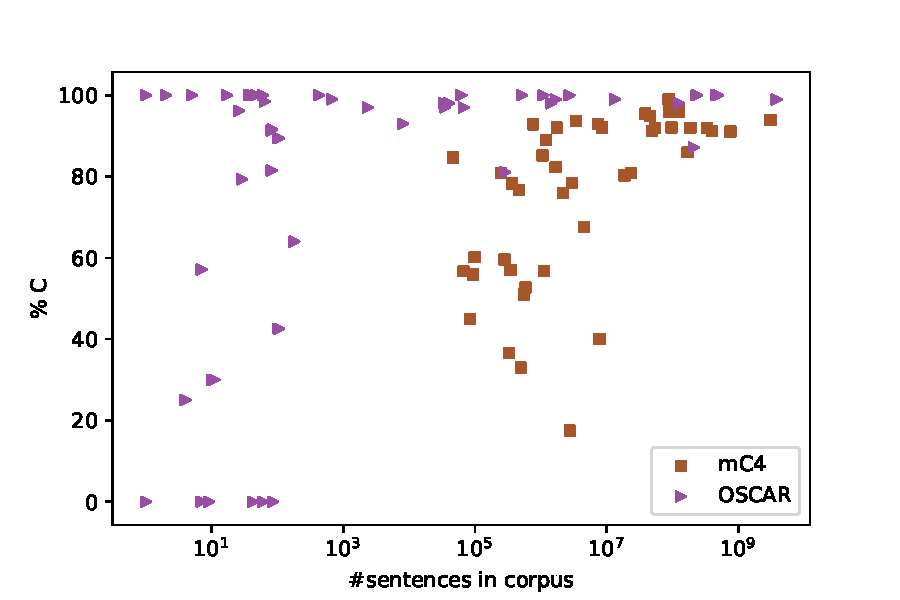
\includegraphics[width=\linewidth]{static/media/data/quality/C_mono.pdf}
        \caption{Monolingual corpora}
        \label{fig:C_mono}
    \end{subfigure}%
    \begin{subfigure}{.5\textwidth}
        \centering
        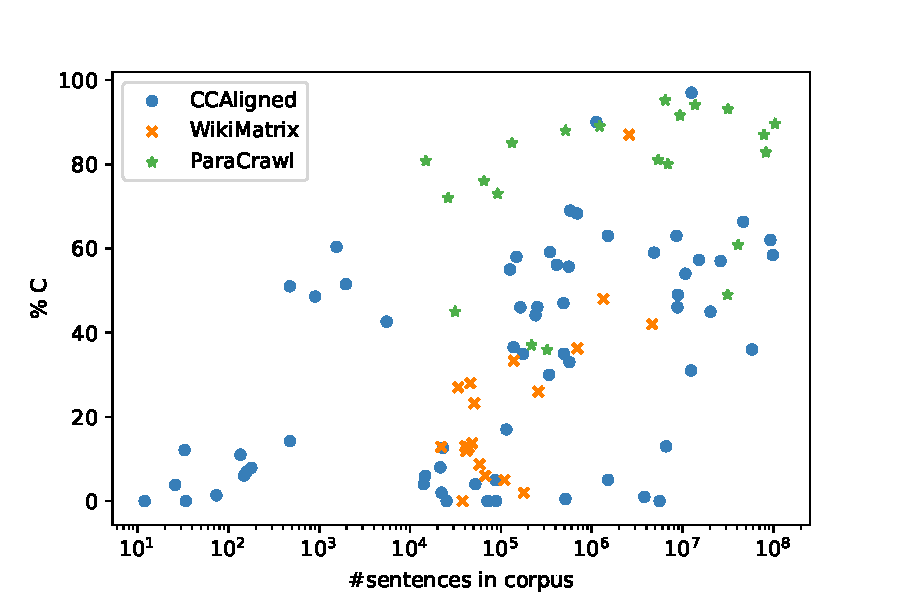
\includegraphics[width=\linewidth]{static/media/data/quality/C_para.pdf}
        \caption{Parallel corpora}
        \label{fig:C_para}
    \end{subfigure}
    \caption{Percentage of sentences labeled as correct vs. log N sentences for all audited languages.}
    \label{fig:C}
\end{figure*}

\begin{figure}[th]
    \centering
    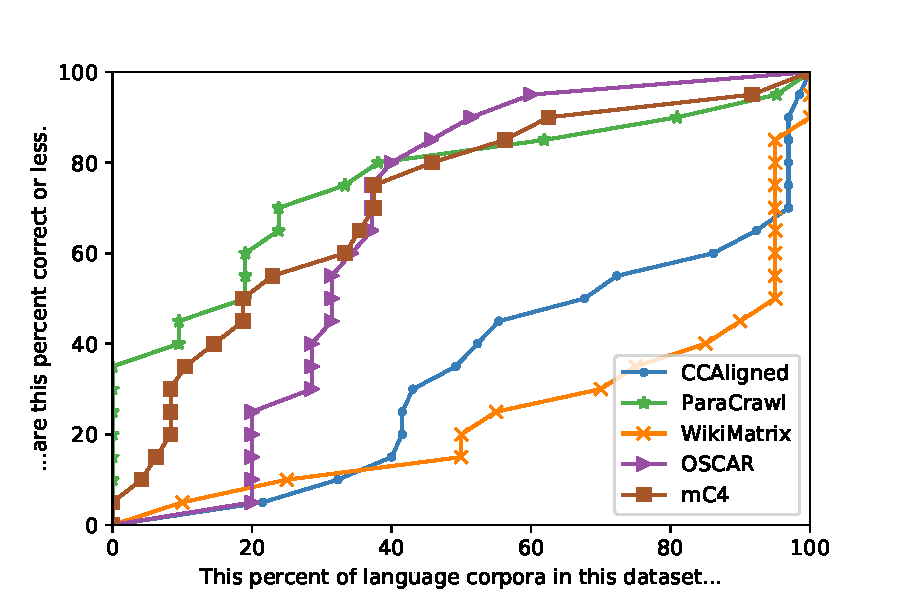
\includegraphics[width=\columnwidth]{static/media/data/quality/num_C_ratio.pdf}
    \caption{Fraction of languages in each dataset below a given quality threshold (percent correct).}% The larger the AUC, the better.}
    \label{fig:ratio_c}
\end{figure}


%In order to verify if lower-resource languages in particular have lower quality, we compare the overall rates with the mean quality of the smallest 20\% and 50\% of languages. We observe that the quality for the 20\% smallest languages is much smaller than the overall mean, especially for CCAligned with a difference of 14\% points. The amount of incorrect translations (but in the right language) is also higher for the smallest languages (32\% point for the smallest 50\%). For OSCAR, the drop in quality is not as pronounced, because it has overall lower quality. MC4 and OSCAR differ by 20\% points overall, but their quality on the smallest 20\% is comparable.
%From this comparison we conclude that \emph{the quality for the least represented languages in the multilingual mix is considerably lower, even more so when the corpus is parallel.}

\paragraph{Which languages have the lowest quality?} Across datasets we observe that the quality is particularly poor for languages that are included in the datasets in romanized script, but are more commonly written in other scripts, e.g., Urdu (\texttt{ur}), Hindi (\texttt{hi}), Arabic (\texttt{ar}). %, Chinese (\texttt{zh}), Telugu (\texttt{te}) and Bulgarian (\texttt{bg}).  
In terms of geography, the poorest quality is found for African languages (\texttt{bm}, \texttt{ff}, \texttt{kg}, \texttt{lg}, \texttt{ln}, \texttt{nso}, \texttt{om}, \texttt{sn}, \texttt{so}, \texttt{tn}, \texttt{wo}), minority languages in Europe and the Middle East that are closely related to higher-resource languages (\texttt{az-IR}, \texttt{frr}, \texttt{nap}, \texttt{szl}, \texttt{zza}), lesser spoken Chinese languages sharing a script with Mandarin (\texttt{yue}, \texttt{wuu}), and four major Austronesian languages (\texttt{bcl}, \texttt{cbk}, \texttt{jv}, \texttt{su}).
%Appendix~\ref{app:stats} contains the detailed per-language statistics for all corpora. 
% Omitted from above: mt

\paragraph{What is the incidence of offensive and pornographic content?}
Overall, the sampled sentences did not contain a large amount of offensive contents. However, there were notable amounts of pornographic content ($>10\%$) found in CCAligned for 11 languages. % not fully annotated: tl_XX, lt_LV ?

%\paragraph{Inter-annotator agreement}
\paragraph{Annotation quality}
For six audited languages from OSCAR and ten from CCAligned we measure the accuracy of the labels assigned by non-proficient speakers against the labels assigned by proficient speakers for all audited sentences. With the full 6-class taxonomy we find a mean accuracy of 0.66
%($\sigma^2 =0.02$) 
for CCAligned audits, and 0.98
%($\sigma^2 =0.002$) 
for OSCAR audits (see appendix~\ref{app:agreement} for language-specific results). With a binary taxonomy distinguishing \texttt{C} from the rest, the accuracy further increases to 0.79
%($\sigma^2=0.01$) 
for CCAligned. This provides strong evidence that good quality annotations are not limited to those proficient in a language.

\subsection{Automatic Filtering}
Given the frequency of \texttt{WL} and \texttt{NL} annotations, it might be tempting to use open-source LangID models to post-filter data on a per-sentence(-pair) level, as OSCAR does. Unfortunately, this turns out to have its own issues.

\paragraph{Sentence-level n-gram filtering}
We classify all sentence pairs of CCAligned with CLD3. By comparing its predictions to the audit labels, we evaluate its quality on the subset of annotated samples: the classifier should detect both correct languages when the pair is annotated as \texttt{C} and \texttt{X}, and should detect incorrect languages in the pair when \texttt{WL} and \texttt{NL}. On this task, the CLD3 classifier
%\footnote{\texttt{filter=0.976 Prec, 0.962 Rec, 0.969 F1.}} 
achieves an average precision of only 40.6\%. %,
%n average accuracy of 56.4\% against our annotators across all audited sentences, 
%underlining the issues with LangID on web domain data~\citep{caswell-etal-2020-language}. %Its recall for detecting those pairs with wrong language(s) is 77.8\%, and its precision 35.9\%. 

\paragraph{Transformer-based LangID filtering}
N-gram LangID models like CLD3 have known problems. However, \citet{caswell-etal-2020-language} demonstrate that semi-supervised transformer-based LangID models strongly out-perform them. We train a comparable transformer-based LangID model and apply it to our annotated CCAligned data. We find that filtering noisy corpora ($<$ 50\% correct) on LangID for both source and target leads to gains in median precision, rising from 13.8\% pre-filter to 43.9\% post-filter. However, this comes at a steep cost of 77.5\% loss in recall.
The biggest winners were Lingala, whose precision climbs from 8\% to 80\%, and Oromo, which soars from 2\% to 33\% in-language. Both of these, however, come at the cost of losing 50\% of the correct in-language sentences. The moral is that, at least at the current stage, there is no one-size-fits-all approach for sentence-level LangID.


\section{Dataset Mis-labeling}
\label{sec:codes}

% Besides general data quality issues, we found a range of problems and inconsistencies with language codes, ranging from serious mislabelings to small transgressions against standard conventions. 

%In order to use data for any practical application, it is important to have a 
Standardized and unambiguous representations of language codes are important for practical data use and exchange. The standard for unambiguous language codes used by most academic and industry applications is BCP-47~\citep{phillips2006tags}, which would  enhance transparency and interoperability if adopted consistently. % since it allows to add subtags for scripts or regional varieties. 
%, which builds off the two-letter ISO639-2 codes and three-letter ISO639\nobreakdash-3 codes. Codes may additionally specify ISO15924 script subtags to indicate that a nonstandard script is used (e.g. \texttt{hi-Latn} for Hindi written in Latin script), ISO3166-1 country codes to indicate regional varieties (e.g. \texttt{fr-CA} for Canadian French), or extensions for private use (e.g. \texttt{ca-x-val} for Valencian Catalan). Some BCP-47 codes represent groups of languages---for instance, \texttt{kg} represents the Kongo language, and \texttt{kng}, \texttt{ldi}, \texttt{kwy}, and \texttt{yom} represent particular varieties of Kongo.

We find a variety of errors in language code usage, ranging from serious mislabelings to small transgressions against standard conventions. . For this analysis, we also include the JW300~\citep{agic-vulic-2019-jw300} dataset, a multilingual dataset crawled from \url{jw.org}. %, which was otherwise not audited in this paper. 
In summary, we find 8 nonstandard codes in CCAligned, 3 in OSCAR, 1 in mC4, 1 in WikiMatrix, and 70 in JW300, for 83 in total. This does not include the 59 codes affected by superset issues. %0 in ParaCrawl, 
Full details are given in appendix~\ref{app:jw300}.
% \subsection{Inconsistent Language Codes}

% One consistent issue is the inconsistent use of language codes. For instance,

\paragraph{Inconsistent Language Codes} One common issue is simply using nonstandard or invented codes. For example, CCAligned uses only two-letter codes, so when the BCP-47 code for a language is three letters it is either shortened (e.g. \texttt{zza} $\rightarrow$ \texttt{zz})
%, \texttt{szl}  $\rightarrow$ \texttt{sz}, \texttt{nso}  $\rightarrow$ \texttt{ns}, \texttt{ckb}  $\rightarrow$ \texttt{cb}, \texttt{ber}  $\rightarrow$ \texttt{tz} \footnote{Tamazight (BCP-47 ber) goes by various codes, so this may have been a shortening of e.g. \texttt{tzm}}) 
or invented (\texttt{shn}  $\rightarrow$ \texttt{qa})
%, \texttt{kac}  $\rightarrow$ \texttt{qd}, \texttt{ceb}  $\rightarrow$ \texttt{cx}), which can lead to 
%this can lead to confusion and limits the compatibility with other tools and resources.
Similarly, OSCAR contains data labeled as \texttt{als} (BCP-47 for Tosk Albanian) that is actually in \texttt{gsw} (Allemanic).
%\footnote{This is a result of the language code used by the Alemanic Wikipedia, and affects any corpus or tool that uses Wikipedia data without correcting for this, like FastText.} 
% \citep{joulin-etal-2017-bag, joulin-etal-2016-fasttext}.
%\footnote{\url{https://en.wikipedia.org/wiki/Alemannic_Wikipedia}
% And in JW300~\citep{agic-vulic-2019-jw300}, a multilingual dataset otherwise not audited in this paper, there are five codes ({\tt cat}, {\tt daf}, {\tt que}, {\tt nya}, {\tt run}) which use ISO693-3 instead of BCP-47 codes. Puzzlingly, in most of these cases there exist separate datasets for the equivalent ISO693-2 and 3 codes (e.g. both {\tt ny} and {\tt nya}).
22 additional language codes in JW300 have similar issues,
%mostly from mis-parsed private-use extensions, 
including 12 codes that start with \texttt{jw\_} but are not %(as they may appear)
Javanese.

% \subsection{False Language Codes}

\paragraph{False sign languages}
12\% (48/417) of JW300
%has a much stranger problem than nonstandard codes. It has the peculiar issue that a full 12\% (48/417) of the languages it claims to cover 
carry language codes for sign languages. %While it is possible to transcribe sign languages using glosses, this is not what these corpora are. 
Instead of sign language transcripts they are texts in another high resource language, mostly English or Spanish---for example, the \texttt{en-zsl} data is actually English-English parallel data (i.e. copies). %Details are in appendix table~\ref{tab:signlanguages}.


\paragraph{Mysterious supersets}
When datasets contain language codes that are supersets of other language codes, it is difficult to determine which particular language the data are in. WikiMatrix has Serbian (\texttt{sr}), Croatian (\texttt{hr}), Bosnian (\texttt{bs}), and Serbo-Croatian (\texttt{sh})---their superset. %\footnote{https://iso639-3.sil.org/code/hbs} 
%. And while there may be some debate whether \texttt{bs},  \texttt{hr},  \texttt{cnr},  and \texttt{sr} are different languages, \texttt{sh} (\texttt{hbs}) is by definition a superset of all of them.\footnote{https://iso639-3.sil.org/code/hbs} 
%The issue of codes that are supersets of others is common enough to include a small table dedicated to it, which we have done with appendix table~\ref{tab:supersets}. 
In some cases this may not be an issue, as with Arabic, where \texttt{ar} conventionally refers to Modern Standard Arabic, even though the code technically encompasses all dialects.
%, or where \texttt{no} typically refers to Norwegian Bokm\r{a}l (\texttt{nb}), though it technically is the superset of \texttt{nb} and \texttt{nn}. 
But in many cases, the nature of the data in the superset code remains a mystery.
% requiring detective work.


\paragraph{Deprecated codes} Finally, there are several deprecated codes that are used: \texttt{sh} in Wikimatrix, \texttt{iw} in mC4, \texttt{sh} and \texttt{eml} in Oscar, and \texttt{daf} in JW300.

% Maybe this is also out of the scope
% TODO the case of simple English in Wikipedia, as well as other languages with well known quality problems in Wikipedia: Buryat, Scots , Waray (bot), Swedish (bot), Cebuano (bot), ...

% a discussion on the issues of dialects might fit better in a paper focused on general problems of multilingual NLP, so maybe we can cut it from here to keepo the story more focused
% Stella: Makes sense to me, especially as length is challenging. I might try to work a sentence about this into the intro, but I'm planning on not writing a paragraph on this.
% TODO Stella: Languages are dialects with an army and a navy: Chinese, BCS, Arabic, Hindi/Urdu/Hindustani, Corsican/Italian/Sicilian

% doesn't ad enough; let's cut 
% Furthermore, language that have little standardized form, barely occur in writing or subsume a lot of diverse dialects, like for example Wu Chinese, have little hope of being correctly classified and adequately captured by automatic crawls, so their quality is expectedly low. 

\section{Risks of Low-Quality Data}\label{sec:risk}
% \section{Risks of Multilingual Data Releases with Low Quality}\label{sec:risk}

%Although releasing a dataset with low or no in-language content may seem innocuous enough, 
%There are several potentially harmful consequences of data releases without sufficient quality checks (or under false labels) that we would like to highlight.

\paragraph{Low quality in downstream applications}
Text corpora today are building blocks for many downstream NLP applications like question answering and text summarization---for instance, a common approach is to first train translation models on such data and then automatically translate training data for downstream models~\citep{conneau-etal-2018-xnli}. If the data used for the original systems is flawed, derived technology may fail for those languages far down the line without knowing the causes.
% The human inspection and auditing of e.g. trained vector representations to detect possible risks and misrepresentations of a subset of languages is arguably harder than manually inspecting a few samples as we did in this work.
% As our analysis has shown, low-resource languages are disproportionately affected by such problems in automatic data curation pipelines.

% \textsc{translate-train} and \textsc{translate-test} paradigms \citep{conneau-etal-2018-xnli}

\paragraph{Representation washing}
Since there are datasets which contain many low-resource languages, the community may feel a sense of progress and growing equity, despite the actual quality of the resources for these languages. %However, models often still perform poorly on NLP tasks for these languages
%Because there appear to be datasets for low-resource languages, the community may collectively feel as though progress is being made in these areas. 
Similarly, if low-quality datasets are used as benchmarks they may exaggerate model performance, making low-resource NLP appear more solved than it is---or conversely, if models perform poorly when trained with such data, it may be wrongly assumed that the task of learning models for these languages is harder than it actually is or infeasible given current resources. These effects could result in productive effort being redirected away from these tasks and languages.
%The result can be that productive effort will be directed away from these fields.

\paragraph{Trust in incorrect ``facts''} % and trust} %, algorithmic trust and automation bias}
We found many instances of parallel-looking sentences that are actually not semantically similar (appendix table~\ref{tab:not_actually_parallel}). They can cause models to produce plausible ``translations" that are factually wrong, but users may still trust them (\textit{algorithmic trust}) without verifying the information. %This is relevant for \textit{algorithmic trust}, when users increasingly trust the outputs of computers and ``algorithms" without verifying the information. 
Similarly, \textit{automation bias} \citep{skitka1999does},
%from social psychology which refers to the bias of 
referring to humans favoring decisions made by automated systems over decisions made by humans, might amplify the issues of inaccurate translations caused by misaligned sentences.
%One variant of this issue that occurs frequently in some datasets is pornographic content.
%, which in the majority of the cases we observed were parts of misaligned sentence pairs. 
%Another effect is that models trained on misaligned pornographic content may hallucinate such content, which may be disturbing to users.


\section{Future Work}
There are a variety of ways to improve both the ease and accuracy of human evaluation, as well a few classes of issues we ignored in this paper, like close dialects. We present a slightly improved suggested rubric in appendix~\ref{app:improved}.

Ideally there can be a standard suite of automatic metrics for datasets, but more study is necessary to determine what the appropriate metrics would be. One important area missing from our analyses however is the estimated portion of a dataset which has been generated by MT,  LM systems, or bots/templates. %A prominent example is the Lsjbot\footnote{\url{https://en.wikipedia.org/wiki/Lsjbot}} which is responsible for creating 80-90\% of content for Swedish, Cebuano and Waray Wikipedia. 
The information captured in machine-generated content might still be useful for modeling, but might falsely overrepresent typical generation patterns and introduce linguistic errors or unnatural artifacts.
% Malagasy wiktionary audit: https://meta.wikimedia.org/wiki/Requests_for_comment/Large-scale_errors_at_Malagasy_Wiktionary
%https://www.vice.com/en/article/4agamm/the-worlds-second-largest-wikipedia-is-written-almost-entirely-by-one-bot

% Finally, similar studies to this in future would do well ton work more on calibrating human raters, to ensure consistent use of error categories.

% An issue that arises with the progress in building technology for some of the languages is the retrieval of machine-generated output as in-language data. This is prominent for mid- to high-resource languages for which translation systems have reached sufficient quality for website translation, as we observed for example a significant amount of translations for Ukrainian. Non-native speakers might not have noticed them during annotations, so the problem might be even larger than we might estimate now. We leave a systematic investigation to future work. A more unexpected artifact is the retrieval of published BPE vocabularies for a range of low-resource languages, such as Sundanese.\footnote{\url{https://nlp.h-its.org/bpemb/su/su.wiki.bpe.vs100000.vocab}}

\section{Conclusion \& Recommendations}\label{sec:recommendation}

Of the five multilingual corpora evaluated, we consistently found severe issues with quality, especially in the lower-resource languages. We rated samples of 205 languages, and found that 87 of them had under 50\% usable data, with a full 15 languages at 0\% in-language. We furthermore found consistent issues with mislabeled data and nonstandard language codes, particularly in the JW300 dataset, and identified 83 affected corpora, at least 48 of which were entirely spurious (Section \ref{sec:codes}). While there might have been anecdotal evidence of insufficient quality for some of the datasets, the majority of these quality issues had not been reported, nor been investigated in depth. These issues might go unnoticed for languages that are not represented in the evaluation of the crawling methods, and cause harm in downstream applications.
% In addition to quality issues we found a wide range of issues with language codes, particularly in JW300 and CCAligned, including mis-labeled data, invented codes, deprecated codes, and superset relations between language codes. %with a particular focus on low-resource languages, which are generally under-evaluated in NLP.

We therefore strongly recommend looking at samples of any dataset before using it or releasing it to the public. As we have shown, one does not need to be proficient in a language to see when there are serious quality issues, and a quick scan of 100 (or fewer!) sentences can be sufficient to detect major problems. Moreover, going through and annotating a small sample of data can bring useful insights about new ways to filter or use it.

If data quality issues are found, a wide variety of techniques can be explored, like filtering on length-ratio, LangID, TF-IDF wordlists \cite{caswell-etal-2020-language} or dictionaries~\citep{kamholz-etal-2014-panlex}; to neural approaches like LM scoring \cite{axelrod-etal-2011-domain,moore-lewis-2010-intelligent,wang2018denoising}. Unfortunately, none of these provides a quick and easy fix, especially for low-resource languages -- data cleaning is no trivial task!

Noisy datasets are however by no means useless, at least if they contain some usable content. Therefore an alternative to filtering can be documentation~\citep{bender2021dangers}. This can take the form of a per-language quality score and notes about known issues,
% ({ \it``language xx has high percentage non-linguistic content'' } etc.), 
a datasheet \citep{gebru2018datasheets} or nutrition label \citep{holland2018dataset}. However, we suggest researchers not release corpora with near-zero in-language content, as this may give the mistaken impression of usable resources.
%even where that is not actually the case.

Finally, we encourage the community to continue conducting evaluations and audits of public datasets -- similar to system comparison papers.
%-- which would help anyone interested in using these datasets for practical purposes.

% \begin{itemize}
%     \item \textbf{LangID Filtering:} As we have seen in Section \ref{sec:audit-res}, wrong-language is a very large class of errors. Per-sentence LangID filtering is a fast and straightforward way to alleviate this, but behaves differently on different languages and often has a high recall cost. As explored in \citet{caswell-etal-2020-language}, LangID models suffer from a variety of pathologies for long-tail languages, and datasets like OSCAR that apply per-sentence n-gram LangID still have wrong-language issues. However, datasets that apply no such filtering, like sentence-level CCAligned, seem to have a much higher proportion of wrong-language. In sum, although there is much headroom, there is also much work that needs to be done.
%     \item \textbf{Nonlinguistic Content Filtering:} LangID filtering will ideally help with this, but this is also not an easy task in general. However, a quick glance through one's data will often reveal particular classes of non-linguistic noise (like URLs, JavaScript, highly repeated characters and {\tt U+FFFD REPLACEMENT CHARACTER}s) that are easy to remove.
%     \item \textbf{Lexicon and Dictionary filtering} For higher linguistic precision, one can filter monolingual data with lexicons \cite{caswell-etal-2020-language} or parallel dictionaries with word-to-word dictionaries~\citep{kamholz-etal-2014-panlex}, and accept sentences/sentence pairs that meet some minimum threshold.
%     A similar approach can be used to filter out pornographic content, although word matching with existing lists such as the one used to create the Switch-C training corpus\footnote{https://github.com/LDNOOBW/List-of-Dirty-Naughty-Obscene-and-Otherwise-Bad-Words/blob/master/en} has been found to also aggressively filter out legitimate content on sexual health and education and LGBTQ advocacy, which can be a source of representational harm \cite{hovy-spruit-2016-social}.
%     In the datasets observed in this paper, it seemed as though a url-based exclusion approach could be more effective; and alternatively to filtering, the data can be let as-is with a disclaimer as in~\citet{gao-etal-2020-the}. 
%     \item \textbf{Fancier approaches:} There is a rich literature on neural filtering approaches. These are certainly very effective, though will likely have to be tuned for low-resource languages. However, we want to stress that much simpler approaches will get a person most of the way to a cleaner dataset.
%     \item \textbf{Consulting native speakers:} Although this is the gold standard, it will unfortunately not be feasible for every language in a large dataset, or for researchers without access to volunteers or crowdworkers in these languages; and, as outlined above, the majority of checking and filtering can be done by non-native speakers. Nonetheless, researchers wishing to provide high-quality data that can be trusted for high-stakes applications will benefit from consulting speakers of the languages they hope to include in their datasets.
%     \item \textbf{Non-English pivot:} Replacing English with another high-resource language which historically co-exists with a low-resource language with a community of bilingual speakers, e.g. crawling a French-Breton corpus would have been arguably a more successful endeavour than English-Breton, and the same may be true for Spanish-Basque vs. English-Basque.


%     TODO: discuss that we selected English-paired subsets, non-English centric MT: https://arxiv.org/abs/2010.11125 https://arxiv.org/abs/2010.10239, https://www.statmt.org/wmt20/pdf/2020.wmt-1.64.pdf
% \end{itemize}

%\section*{Acknowledgements}
%We would like to thank the AfricaNLP and Google reviewers who have helped us shape this paper. Furthermore, we are grateful for Ahmed El-Kishky's support and help with CCAligned and WikiMatrix size statistics.



\section{Details on Language Code Issues}
\label{app:jw300}

Section \ref{sec:codes} describes a variety of issues surrounding language codes that are unclear or incorrect. This section provides more details, focusing on the JW300 dataset.

In table \ref{tab:supersets} we provide a complete table of the datasets where one code is defined as a superset of the other by the ISO standard, and in table \ref{tab:signlanguages} we provide a complete list of the language codes in JW300 which purport to be sign language but are actually unrelated high-resource languages.

Special attention needs to be given to the JW300 dataset, which, in addition to the sign languages and superset code issues, has a variety of other peculiarities. These problems seem to originate in the codes used by jw.org\footnote{The jw.org website seems to use correct BCP-47 extensions now, however, and entering a code such as ``jw\_dmr" redirects to ``naq\_x\_dmr" }, which were apparently not checked in the creation of the JW300 dataset. An overview is provided in Table \ref{tab:jw300nonbcp}, and the following paragraphs give specifics.

Twelve languages in JW300 have codes starting in \texttt{jw\_}, suggesting they are varieties of Javanese (ISO639-1 \texttt{jw}), but are instead attempts to represent language dialects for which there are not BCP-47 codes. These codes seem to have been updated in jw.org to appropriate BCP-47 private-use extensions in the form \texttt{<supercode>\_x\_<tag>}, which are provided in Table \ref{tab:jw300nonbcp}.

In addition to the \texttt{jw\_} tags, there are two other mis-used private subtags: \texttt{hy\_arevmda}, which in addition to lacking the mandatory \texttt{\_x\_} appears to represent standard Western Armenian (\texttt{hyw}); and \texttt{rmy\_AR}, which, rather than being Romany from Argentina, is Kalderash Romany.

There are also a few anomalies where private use extensions should have been used but other methods were found to convey the distinctions. Three codes appear in addition to equivalent ISO codes, making it unclear which languages they are. Two of these are equivalencies between  ISO639-2 and  ISO639-3 (\texttt{nya} and \texttt{ny} are both Chichewa, \texttt{qu} and \texttt{que} are both Quechua). and one is a script equivalency (\texttt{kmr} and \texttt{kmr\_latn} are both in Latin script). In these three cases the two codes do represent different languages --- so a private use extension would have been appropriate.

Finally, there is the more minor issue that three languages use the ISO639-3 code instead of the ISO639-2 code, and therefore are not BCP-47.


In addition to the JW300-specific tables, Table \ref{tab:misc_codes} summarizes misc errors in CCAligned and OSCAR that were detailed in Section \ref{sec:codes}.

\begin{table*}[t]
    \centering
    \begin{tabular}{lll}
        \toprule
        Dataset    & supercode & subcode(s)                      \\
        \hdashline
        JW300      & kg        & kwy                             \\
        JW300      & mg        & tdx                             \\
        JW300      & qu        & que,qug,qus,quw,quy,quz,qvi,qvz \\
        JW300      & sw        & swc                             \\
        \hdashline
        OSCAR      & ar        & arz                             \\
        OSCAR      & az        & azb                             \\
        OSCAR      & sh        & bs,hr,sr                        \\
        OSCAR      & ku        & ckb                             \\
        OSCAR      & ms        & id,min                          \\
        OSCAR      & no        & nn                              \\
        OSCAR      & sq        & als$^{*}$                       \\
        OSCAR      & zh        & yue,wuu                         \\
        %  \hdashline
        % Tatoeba & ar & acm,afb,ajp,apc,arq,ary,arz,ayl \\
        % Tatoeba & ber & kab \\
        % Tatoeba & et & vro \\
        % Tatoeba & ku & ckb,kmr,sdh \\
        % Tatoeba & lv & ltg \\
        % Tatoeba & sq & aln \\
        \hdashline
        Wikimatrix & ar        & arz                             \\
        Wikimatrix & sh        & bs,hr,sr                        \\
        Wikimatrix & zh        & wuu                             \\
        \bottomrule
    \end{tabular}
    \caption{Situations where two language codes are represented, but one is a superset of another by the ISO standard, leading to unclarity about the data in the supercode dataset. $^{*}$The \texttt{als} dataset is actually in \texttt{gsw}.}
    \label{tab:supersets}
\end{table*}



\begin{table*}[t]
    \centering
    \begin{tabular}{ll}
        \toprule
        Actual language & Code in JW300                       \\
        \hdashline
        cs              & cse                                 \\
        de              & gsg                                 \\
        el              & gss                                 \\
        en              & ase,asf,bfi,ins,psp,sfs,zib,zsl     \\
        es              & aed,bvl,csf,csg,csn,csr,ecs,esn,    \\
                        & gsm,hds,lsp,mfs,ncs,prl,pys,ssp,vsl \\
        fi              & fse                                 \\
        fr              & fcs,fsl                             \\
        hu              & hsh                                 \\
        id              & inl                                 \\
        it              & ise                                 \\
        ja              & jsl                                 \\
        ko              & kvk                                 \\
        pl              & pso                                 \\
        pt              & bzs,mzy,psr,sgn\_AO                 \\
        ro              & rms                                 \\
        ru              & rsl                                 \\
        sk              & svk                                 \\
        sq              & sql                                 \\
        st              & jw\_ssa                             \\
        zh              & csl,tss                             \\
        \bottomrule
    \end{tabular}
    \caption{There are 48 languages in the JW300 corpus with language codes that correspond to sign languages, but in reality are unrelated high-resource languages (usually the most spoken language in the country of origin of the sign language). This table shows the actual language of the data corresponding to each sign language code.} %  For instance, the \texttt{ase-en} parallel data is actually \texttt{en-en} parallel data (copied source and target).
    \label{tab:signlanguages}
\end{table*}



\begin{table*}[th]
    \centering
    \begin{tabular}{lll}
        \toprule
        \textbf{Code in JW300} & \textbf{BCP-47 code} & \textbf{Actual Language Name} \\
        \multicolumn{3}{c}{}                                                          \\
        \multicolumn{3}{c}{\textbf{Incorrect private-use extensions}}                 \\
        \hdashline
        hy\_arevmda            & hyw                  & Western Armenian              \\
        jw\_dgr                & os\_x\_dgr           & Digor Ossetian                \\
        jw\_dmr                & naq\_x\_dmr          & Damara Khoekhoe               \\
        jw\_ibi                & yom\_x\_ibi          & Ibinda Kongo                  \\
        jw\_paa                & pap\_x\_paa          & Papiamento (Aruba)            \\
        jw\_qcs                & qxl                  & Salasaca Highland Kichwa      \\
        jw\_rmg                & rmn\_x\_rmg          & Greek Romani (South)          \\
        jw\_rmv                & rmy\_x\_rmv          & Vlax Romani, Russia           \\
        jw\_spl                & nso\_x\_spl          & Sepulana                      \\
        jw\_ssa                & st\_ZA               & Sesotho (South Africa)        \\
        jw\_tpo                & pt\_PT               & Portuguese (Portugal)         \\
        jw\_vlc                & ca\_x\_vlc           & Catalan (Valencia)            \\
        jw\_vz                 & skg\_x\_vz           & Vezo Malagasy                 \\
        rmy\_AR                & rmy\_x\_?            & Kalderash                     \\

        \multicolumn{3}{c}{}                                                          \\
        \multicolumn{3}{c}{\textbf{Equivalent codes used in place of extensions}}     \\
        \hdashline
        kmr\_latn              & kmr\_x\_rdu          & Kurmanji (Caucasus)           \\
        nya                    & ny\_x\_?             & Chinyanja (Zambia)            \\
        que                    & qu\_x\_?             & Quechua (Ancash)              \\

        \multicolumn{3}{c}{}                                                          \\
        \multicolumn{3}{c}{\textbf{Deprecated codes}}                                 \\
        \hdashline
        daf                    & dnj/lda              & Dan                           \\
        % sgn\_AO & 	pt & 	Portuguese \\ 

        \multicolumn{3}{c}{}                                                          \\
        \multicolumn{3}{c}{\textbf{ISO-693-3 used in place of ISO-693-2}}             \\
        \hdashline
        cat                    & ca                   & Catalan                       \\
        gug                    & gn                   & Guarani                       \\
        run                    & rn                   & Kirundi                       \\
        tso\_MZ                & ts\_MZ               & Changana (Mozambique)         \\
        \bottomrule
    \end{tabular}
    \caption{Language code issues in the JW300 datasets for 22 language varieties not covered by Tables \ref{tab:supersets} and \ref{tab:signlanguages}. Twelve languages have codes starting in \texttt{jw\_}, suggesting they are varieties of Javanese, but are instead mis-parsed private-use extensions. Three codes appear in addition to equivalent ISO codes, making it unclear which languages they are. One language uses a deprecated ISO code. Four languages use the ISO639-3 code instead of the ISO639-2 code, and therefore are not BCP-47. (Note: in this table, private use extensions are given as they appear in jw.org, and specified as `?' if they are absent from jw.org.)}
    \label{tab:jw300nonbcp}
\end{table*}



\section{Complete Error Taxonomy and Instructions}

In addition to the table given in table \ref{tab:examples}, raters were provided with the following verbal notes on the error codes
\begin{itemize}
    \item \textbf{\texttt{CC}: Correct translation, natural sentence:} It's OK if it's a sentence fragment instead of a whole sentence, as long as it is not too short (about 5 words or greater). The translation does not have to be perfect.
    \item \textbf{\texttt{\texttt{CS}}: Correct Translation, but single word or short phrase:} Also includes highly repeated short phrases, like ``the cat the cat the cat the cat the cat ..."
    \item \textbf{\texttt{CB}: Correct translation, but boilerplate: } This can be auto-generated or formulaic content, or content that one deems ``technically correct but generally not very useful to NLP models". Unfortunately, it's often not clear what should be counted as boilerplate...do your best.
    \item \textbf{\texttt{X}: Incorrect translation} [for parallel sentences] both source and target are in the correct language, but they are not adequate translations.
    \item \textbf{\texttt{WL}: Wrong language} For short sentences, especially with proper nouns, there is often a fine line between ``Wrong language" and ``Not language". Do your best.
    \item \textbf{\texttt{NL}: Not language} At least one of source and target are not linguistic content. Any sentence consisting only of a proper noun (e.g. ``Tyrone Ping") should be marked as \texttt{NL}.
    \item \textbf{\texttt{U}: Unknown} for sentences that need verification by a native speaker. This is an auxiliary label that is resolved in most cases.
\end{itemize}

%Additionally, we provide a few examples of incorrect translations (\texttt{X}) in table \ref{tab:not_actually_parallel} demonstrating common patterns we saw, where sentences have superficial similarity but represent different facts, spelling potential danger for models trained on them.

Finally, for future work please consider using the aspirational error taxonomy in appendix \ref{app:improved}, rather than the one presented above.

\begin{table*}[!htbp]
    \centering
    \resizebox{\textwidth}{!}{%

        \begin{tabular}{lcccccccccccc}
            \toprule
                           & \texttt{es\_XX} & \texttt{bm\_ML} & \texttt{yo\_NG} & \texttt{tr\_TR} & \texttt{ku\_TR} & \texttt{zh\_CN} & \texttt{af\_ZA} & \texttt{jv\_ID} & \texttt{zh\_TW} & \texttt{it\_IT} & \textbf{mean} \\
            \midrule
            \textbf{Acc-6} & 0.58            & 0.73            & 0.41            & 0.45            & 0.43            & 0.55            & 0.65            & 0.55            & 0.46            & 0.55            & 0.66          \\
            \textbf{Acc-4} & 0.77            & 0.73            & 0.60            & 0.55            & 0.56            & 0.72            & 0.72            & 0.57            & 0.58            & 0.66            & 0.72          \\
            \textbf{Acc-2} & 0.91            & 0.96            & 0.72            & 0.64            & 0.71            & 0.79            & 0.77            & 0.92            & 0.81            & 0.69            & 0.79          \\
            \bottomrule
        \end{tabular}%
    }
    \caption{Rater evaluation for a subset of audits from \textbf{CCAligned} (translated from English) measured by the accuracy (Acc-$n$) of labels assigned by non-proficient speaker against those assigned by proficient speakers. $n$ indicates the granularity of the classes.  For $n=6$ all classes of the taxonomy were distinguished, for $n=4$ the \texttt{C} subclasses were combined, and for $n=2$ it is binary decision between \texttt{C} and the rest of the error classes.}
    \label{tab:agreement_ccaligned}
\end{table*}

\clearpage

\begin{table}[!htbp]
    \centering
    \resizebox{\columnwidth}{!}{%

        \begin{tabular}{lccccccccc}
            \toprule
                           & \texttt{tyv} & \texttt{rm} & \texttt{bar} & \texttt{eml} & \texttt{zh} & \texttt{la} & \textbf{mean} \\
            \midrule
            \textbf{Acc-6} & 1.0          & 0.98        & 1.0          & 1.0          & 0.86        & 1.0         & 0.98          \\
            \textbf{Acc-4} & 1.0          & 1.0         & 1.0          & 1.0          & 0.87        & 1.0         & 0.98          \\
            \textbf{Acc-2} & 1.0          & 1.0         & 1.0          & 1.0          & 0.87        & 1.0         & 0.98          \\
            \bottomrule
        \end{tabular}%
    }
    \caption{Rater evaluation for a subset of audits from \textbf{OSCAR} measured by the accuracy (Acc-$n$) of labels assigned by non-proficient speaker against those assigned by proficient speakers.  $n$ indicates the granularity of the classes. For $n=6$ all classes of the taxonomy were distinguished, for $n=4$ the \texttt{C} subclasses were combined, and for $n=2$ it is binary decision between \texttt{C} and the rest of the error classes.}
    \label{tab:agreement_oscar}
\end{table}


\begin{table}[!ht]
    \small
    \centering
    \begin{tabular}{lll}
        \toprule
        corpus     & code in corpus & correct code \\
        \hline
        CCAligned  & zz             & zza          \\
        CCAligned  & sz             & szl          \\
        CCAligned  & ns             & nso          \\
        CCAligned  & cb             & ckb          \\
        CCAligned  & tz             & ber          \\
        CCAligned  & qa             & shn          \\
        CCAligned  & qd             & kac          \\
        CCAligned  & cx             & ceb          \\
        mC4        & iw             & he           \\
        OSCAR      & eml            & egl          \\
        OSCAR      & als            & gsw          \\
        OSCAR      & sh             & hbs          \\
        Wikimatrix & sh             & hbs          \\
        \bottomrule
    \end{tabular}
    \caption{Miscellaneous errors in language codes not in other tables (mentioned in the text in Section \ref{sec:codes}).}
    \label{tab:misc_codes}
\end{table}


\section{Non-proficient Rater Evaluation}\label{app:agreement}

Tables~\ref{tab:agreement_ccaligned} and~\ref{tab:agreement_oscar} show the detailed rating accuracy scores for all selected languages for several levels of annotation granularity. We can see that for the CCAligned data, reducing the labels to a binary scale naturally increases the accuracy (except for \texttt{tr\_TR}), so a binary interpretation (``correct" sentence vs. error) is the most reliable. For monolingual data, the accuracy appears exceptionally high since the \texttt{bar} and \texttt{tyv} corpora contain $<100$ sentences each (4 and 25, respectively).


\begin{table}[!h]
    \small
    \centering
    \begin{tabular}{ll}
        \toprule

        \texttt{en}  & The prime minister of the \textbf{UK} is \textbf{Boris Johnson}.     \\
        \texttt{nl}  & De minister-president van \textbf{Nederland} is \textbf{Mark Rutte}. \\
        \hdashline
        % \texttt{en} &Sunglasses \\
        % \texttt{ig}	&ah\d{i}a Nyocha \\
        % \hdashline
        \texttt{en}  & \textbf{24 March} 2018                                               \\
        \texttt{pt}  & \textbf{14 Novembro} 2018                                            \\
        \hdashline
        % \texttt{en} &The current local time in \textbf{Sarasota} is \textbf{89} minutes ahead of apparent solar time. \\
        % \texttt{nn}	&Den lokale tiden i \textbf{Miami} er \textbf{86} minutt f\o{o}re sann soltid. \\
        \texttt{en}  & The current local time in \textbf{Sarasota} is \textbf{89} minutes.  \\
        \texttt{nn}  & Den lokale tiden i \textbf{Miami} er \textbf{86} minutt.             \\
        \hdashline
        \texttt{en}  & In \textbf{1932} the highway was extended \textbf{north to LA}.      \\
        \texttt{bar} & \textbf{1938} is de Autobahn bei \textbf{Inglstod} fertig gstellt.   \\
        % \hdashline
        % \textit{en:} He was engaged to the lawyer and actor João Lima Junior, with whom he dated from 2004 to 2006. \\
        % \textit{nds:} Ze woont in de tussentied samen met zanger en liedtiesschriever Johannes Oerding met wie ze sinds 2009 ook samen op de bühne stiet.\\
        \bottomrule
    \end{tabular}
    \caption{Examples of ``parallel" data where the translation has a different meaning than the source, but the form looks the same. Such data may encourage hallucinations of fake ``facts".}
    \label{tab:not_actually_parallel}
\end{table}

\section{Not-So-Parallel Data}
Table~\ref{tab:not_actually_parallel} contains a list of examples from the audited datasets that were misaligned  (\texttt{X}). These examples in particular illustrate that structurally similar sentences can easily describe very different facts. Translation models trained on such examples might hallucinate such fact-altering translations.


\section{Quality vs Size}\label{app:plots}
To understand the relation between the amount of data available for each language in each corpus and the quality as estimated by our audit, we plot the ratio of \texttt{X}, \texttt{NL} and \texttt{WL} labels against the number of sentences in figures~\ref{fig:c_app},~\ref{fig:x},~\ref{fig:nl},~\ref{fig:wl}.






\section{Methodological Notes}\label{app:strategies}

A surprising amount of work can be done without being an expert in the languages involved. The easiest approach is simply to search the internet for the sentence, which usually results in finding the exact page the sentence came from, which in turn frequently contains clues like language codes in the URL, or a headline like \textit{News in X language}, sometimes with references to a translated version of the same page. However, for the cases where this is insufficient, here are a few tips, tricks, and observations.

\subsection*{No Skills Required}
Things that do not require knowledge of the language(s) in question.

\begin{enumerate}
    \item ``Not language'' can usually be identified by anyone who can read the script, though there are tricky cases with proper nouns.
    \item Frequently, ``parallel" sentences contain different numbers in the source and target (especially autogenerated content), and are easy to disqualify
    \item Errors tend to repeat. If a word is mistranslated once, it will often be mistranslated many more times throughout a corpus, making it easy to spot
\end{enumerate}

\subsection*{Basic Research Required}
Things that do not require knowledge of the language(s) in question but can be done with basic research.
\begin{enumerate}
    \item If it's written in the wrong script it's considered wrong language. (Sometimes the writing system is indicated in the published corpus, e.g. \texttt{bg-Latn}, but usually the language has a ``default" script defined by ISO.)
    \item Some types of texts come with inherent labels or markers, such as enumerators or verse numbers.
          %For example, much of CCAligned's Odia text is Christian Bible verses, which are preceded by an identifier like ``Matt 12:37". 
    \item When all else fails, search the internet for the whole sentence or n-grams thereof! If the whole sentence can be found, frequently the language is betrayed by the webpage (the language's autonym is useful in this case).
\end{enumerate}



% \subsection{Weak Knowledge}

% Things that can be done by people with weak knowledge of the language(s) or strong knowledge of a related language.

% \begin{enumerate}
%     \item Some types of texts come with inherent labels or markers, such as enumerators or verse numbers. For example, much of CCAligned's Odia text is Christian Bible verses. 
% \end{enumerate}



\begin{figure*}[ht]
    \label{ fig7}
    \begin{minipage}[b]{0.5\linewidth}
        \centering
        \includegraphics[width=\linewidth]{static/media/data/quality/C.pdf}
        \caption{Ratio of \texttt{C} ratings vs size.}
        \label{fig:c_app}
        \vspace{4ex}
    \end{minipage}%%
    \begin{minipage}[b]{0.5\linewidth}
        \centering
        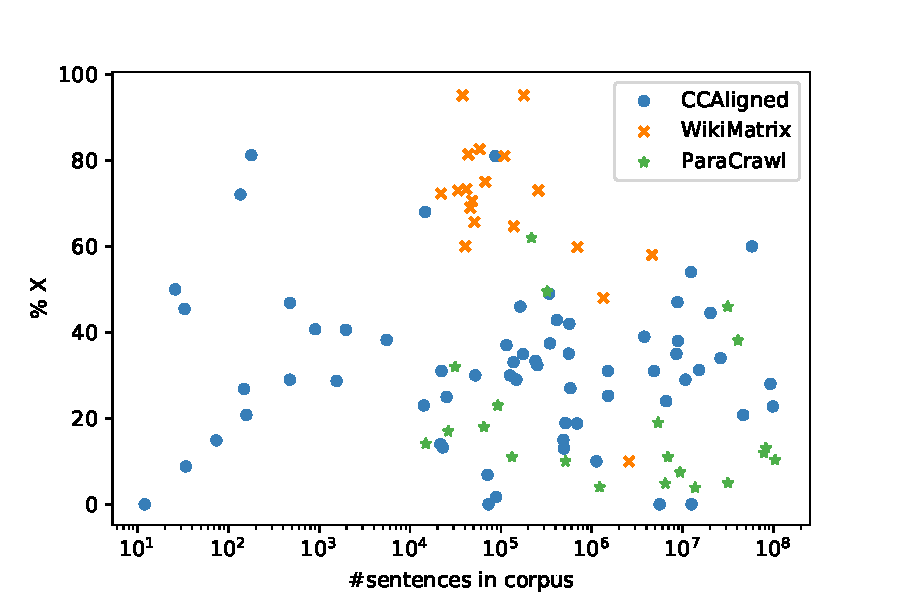
\includegraphics[width=\linewidth]{static/media/data/quality/X.pdf}
        \caption{Ratio of \texttt{X} ratings vs size.}
        \label{fig:x}
        \vspace{4ex}
    \end{minipage}
    \begin{minipage}[b]{0.5\linewidth}
        \centering
        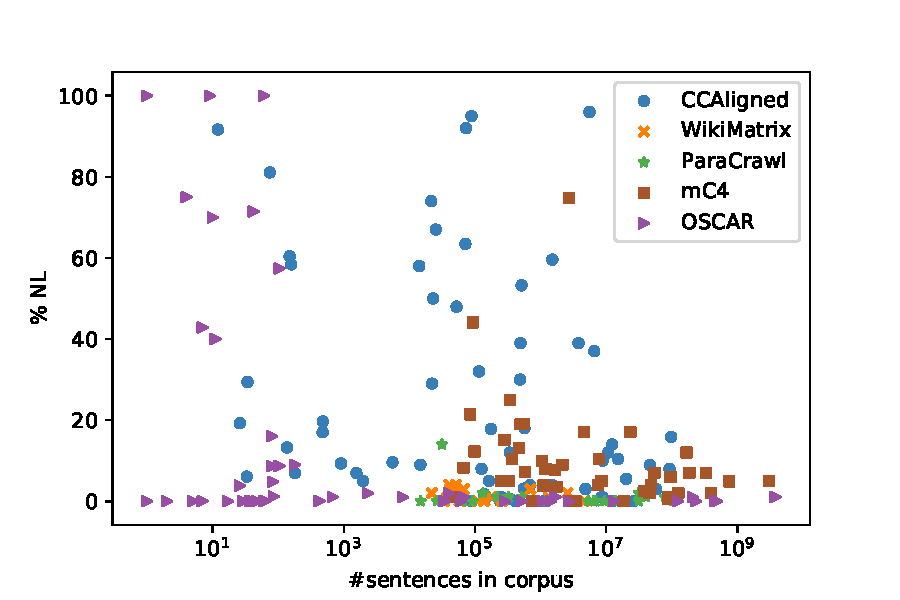
\includegraphics[width=\linewidth]{static/media/data/quality/NL.pdf}
        \caption{Ratio of \texttt{NL} ratings vs size.}
        \label{fig:nl}
        \vspace{4ex}
    \end{minipage}%% 
    \begin{minipage}[b]{0.5\linewidth}
        \centering
        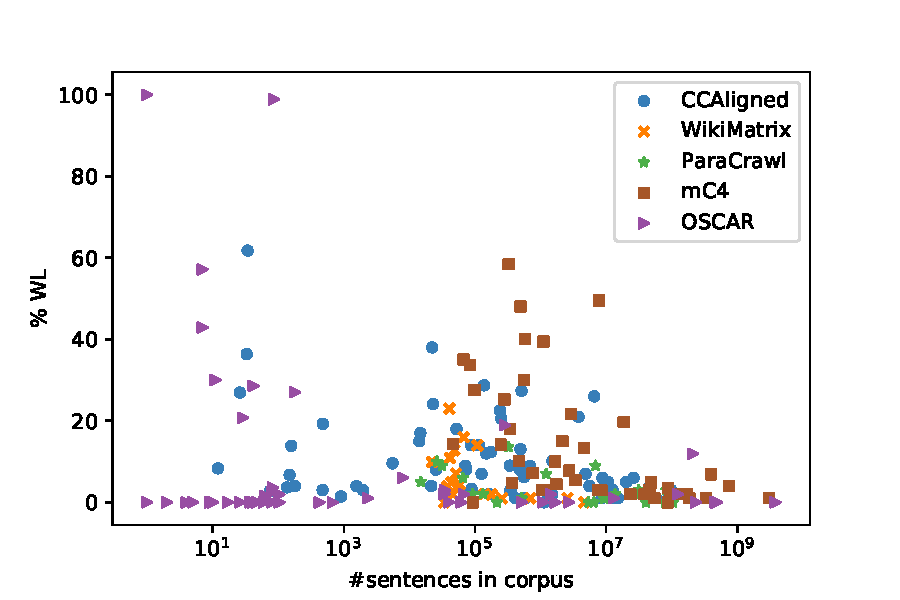
\includegraphics[width=\linewidth]{static/media/data/quality/WL.pdf}
        \caption{Ratio of \texttt{WL} ratings vs size.}
        \label{fig:wl}
        \vspace{4ex}
    \end{minipage}
\end{figure*}


\section{Aspirational Error Taxonomy}
\label{app:improved}

Although the error taxonomy used in this paper did the job, there are a variety of ways to improve both the ease and accuracy of human evaluation, as well as the ease of automatically detecting issues and fixing them. With respect to improved annotations, the error taxonomy presented in this paper lacks at least one significant category of error, namely ``correct/in-language but unnatural".  Similarly, the definition of ``correct-short" and ``correct-boilerplate" were not understood equally by all annotators, leading us to collapse the categories into one for most analyses. Similarly, a concept like ``correct-short" has potential issues for agglutinative languages like Turkish. Finally, it was unclear what to do with related dialects, e.g. when a sentence is ``almost correct but wrong dialect" or when it is unclear which dialect a sentence belongs to.

Therefore, we present here a slightly modified version which we hope is both more explicit and finer-grained. The main changes are 1) replacing ``CB" and ``CS" with a catch-all for lower-quality sentences ``CL", and 2) incorporating two codes for languages with related dialects. This is also by no means a perfect rubric, and would benefit from some fine-tuning and workshopping based on the particular dataset or application in question.

\begin{itemize}
    \item \textbf{\texttt{CC}: Correct:} Natural in-language sentence. It's ok if it has a few small issues, like spelling errors or a few words from another language, or if it’s a sentence fragment of reasonable length (about 5 words or more). For translations, there may be minor mistakes in the translation.
    \item \textbf{\texttt{\texttt{CL}}: Correct Low-quality:} In-language sentence, but low-quality. This could be ungrammatical text, boilerplate, or very short fragments. For translations, this is the appropriate code for a low-quality translation.
    \item \textbf{\texttt{X}: Incorrect translation} [for parallel sentences] both source and target are in the correct language, but they are not adequate translations.
    \item \textbf{\texttt{DW}: Wrong Dialect} \textit{This code is only applicable for dialects that are closely related to other languages/dialects.} This sentence is in a related but different dialect to the language it's supposed to be in. For instance, it's supposed to be in Sa'idi Arabic but it's in Egyptian Arabic.
    \item \textbf{\texttt{DA}: Ambiguous Dialect} \textit{This code is only applicable for dialects that are closely related to other languages/dialects.} Correct but ambiguous whether it's in the correct language. For instance, many short sentences in Gulf Arabic may also be valid in MSA, and many written Cantonese sentences might also be valid in Mandarin.
    \item \textbf{\texttt{WL}: Wrong language} This sentence is not in the language it's supposed to be. For short sentences, especially with proper nouns, there is often a fine line between ``Wrong language" and ``Not language". Do your best.
    \item \textbf{\texttt{NL}: Not language} At least one of source and target are not linguistic content. Any sentence consisting only of a proper noun (e.g. ``Ibuprofin", ``Calvin Klein", or ``Washington DC") should be marked as \texttt{NL}
    \item \textbf{\texttt{U}: Unknown} for sentences that need verification by a native speaker. This is an auxiliary label that is resolved in most cases.
\end{itemize}

\textbf{Special note on Boilerplate:} ``Boilerplate" generally refers to autogenerated text found on websites. It's not always clear when a sentence is boilerplate or not. If you see a lot of similar formulaic sentences in the sample, however, that's a good sign that they are boilerplate, and you can mark them all as ``CL" ! Common types of boilerplate include sentences like ``Convert Euro to Pound", ``Online gambling games", ``Download Game of Thrones Free Torrent" and so on.


\textbf{Special note on Mixed Language:} Some samples are mixed between the right language and some other language. Some out-of-language content is fine, but a majority out-of-language content is not. We can mark the sentence ``CC" if: 1) it is majority in-language, and 2) the in-language portion is more than a short phrase. For unclear border cases you can use “CL”.


\section{Complete Tables}\label{app:stats}
Tables \ref{tab:ccaligned-full}, \ref{tab:mc4-full}, \ref{tab:oscar-full}, \ref{tab:paracrawl-full}, and \ref{tab:wikimatrix-full} give the complete annotation percentages for CCAligned, MC4, OSCAR, Paracrawl, and Wikimatrix, respectively.

%%% CCALIGNED %%%

\begin{table*}[hbt!]
    \centering
    \resizebox*{0.9\textwidth}{!}{ %\textheight}{%
        \begin{tabular}{l|rrrr|rrrr|rr}
            \toprule
            {}                      & C       & CC      & CS      & CB      & X       & WL      & NL      & porn    & \#sentences & avg target length \\
            \midrule
            \textbf{en-sz\_PL}      & 0.00\%  & 0.00\%  & 0.00\%  & 0.00\%  & 0.00\%  & 8.33\%  & 91.67\% & 0.00\%  & 12          & 71.42             \\
            \textbf{en-mt\_MT}      & 3.85\%  & 0.00\%  & 3.85\%  & 0.00\%  & 50.00\% & 26.92\% & 19.23\% & 0.00\%  & 26          & 12.58             \\
            \textbf{en-tz\_MA}      & 12.12\% & 6.06\%  & 6.06\%  & 0.00\%  & 45.45\% & 36.36\% & 6.06\%  & 0.00\%  & 33          & 57.33             \\
            \textbf{en-zz\_TR}      & 0.00\%  & 0.00\%  & 0.00\%  & 0.00\%  & 8.82\%  & 61.76\% & 29.41\% & 0.00\%  & 34          & 46.53             \\
            \textbf{en-kg\_AO}      & 1.35\%  & 0.00\%  & 1.35\%  & 0.00\%  & 14.86\% & 2.70\%  & 81.08\% & 0.00\%  & 74          & 29.20             \\
            \textbf{en-qa\_MM}      & 11.03\% & 5.88\%  & 3.68\%  & 1.47\%  & 72.06\% & 3.68\%  & 13.24\% & 0.00\%  & 136         & 55.28             \\
            \textbf{en-bm\_ML}      & 6.04\%  & 4.03\%  & 2.01\%  & 0.00\%  & 26.85\% & 6.71\%  & 60.40\% & 0.00\%  & 149         & 32.19             \\
            \textbf{en-az\_IR}      & 6.93\%  & 6.93\%  & 0.00\%  & 0.00\%  & 20.79\% & 13.86\% & 58.42\% & 0.00\%  & 158         & 115.85            \\
            \textbf{en-qd\_MM}      & 7.92\%  & 4.95\%  & 1.98\%  & 0.99\%  & 81.19\% & 3.96\%  & 6.93\%  & 0.00\%  & 179         & 60.34             \\
            en-ay\_BO               & 51.00\% & 33.00\% & 18.00\% & 0.00\%  & 29.00\% & 3.00\%  & 17.00\% & 0.00\%  & 475         & 92.19             \\
            \textbf{en-ak\_GH}      & 14.23\% & 13.60\% & 0.63\%  & 0.00\%  & 46.86\% & 19.25\% & 19.67\% & 0.00\%  & 478         & 45.85             \\
            en-st\_ZA               & 48.57\% & 42.14\% & 0.00\%  & 6.43\%  & 40.71\% & 1.43\%  & 9.29\%  & 0.00\%  & 904         & 111.83            \\
            en-ve\_ZA               & 60.40\% & 29.70\% & 21.78\% & 8.91\%  & 28.71\% & 3.96\%  & 6.93\%  & 0.00\%  & 1555        & 82.99             \\
            en-ts\_ZA               & 51.49\% & 34.65\% & 11.88\% & 4.95\%  & 40.59\% & 2.97\%  & 4.95\%  & 0.00\%  & 1967        & 73.93             \\
            en-or\_IN               & 42.61\% & 6.09\%  & 24.35\% & 12.17\% & 38.26\% & 9.57\%  & 9.57\%  & 0.00\%  & 5526        & 71.39             \\
            \textbf{en-ns\_ZA }     & 4.00\%  & 2.00\%  & 0.00\%  & 2.00\%  & 23.00\% & 15.00\% & 58.00\% & 4.00\%  & 14138       & 33.52             \\
            \textbf{en-lg\_UG}      & 6.00\%  & 0.00\%  & 6.00\%  & 0.00\%  & 68.00\% & 17.00\% & 9.00\%  & 2.00\%  & 14701       & 15.83             \\
            \textbf{en-ln\_CD}      & 8.00\%  & 4.00\%  & 3.00\%  & 1.00\%  & 14.00\% & 4.00\%  & 74.00\% & 4.00\%  & 21562       & 28.80             \\
            \textbf{en-om\_KE}      & 2.00\%  & 2.00\%  & 0.00\%  & 0.00\%  & 31.00\% & 38.00\% & 29.00\% & 24.00\% & 22206       & 23.83             \\
            \textbf{en-ss\_SZ}      & 12.65\% & 9.04\%  & 3.61\%  & 0.00\%  & 13.25\% & 24.10\% & 50.00\% & 13.86\% & 22960       & 25.30             \\
            \textbf{en-te\_IN\_rom} & 0.00\%  & 0.00\%  & 0.00\%  & 0.00\%  & 25.00\% & 8.00\%  & 67.00\% & 5.00\%  & 25272       & 24.21             \\
            \textbf{en-cb\_IQ}      & 4.00\%  & 1.00\%  & 3.00\%  & 0.00\%  & 30.00\% & 18.00\% & 48.00\% & 11.00\% & 52297       & 30.04             \\
            \textbf{en-tn\_BW}      & 0.00\%  & 0.00\%  & 0.00\%  & 0.00\%  & 6.90\%  & 8.97\%  & 63.45\% & 10.34\% & 71253       & 16.80             \\
            \textbf{en-ff\_NG}      & 0.00\%  & 0.00\%  & 0.00\%  & 0.00\%  & 0.00\%  & 8.00\%  & 92.00\% & 2.00\%  & 73022       & 33.59             \\
            \textbf{en-sn\_ZW}      & 5.00\%  & 1.00\%  & 3.00\%  & 1.00\%  & 81.00\% & 14.00\% & 0.00\%  & 0.00\%  & 86868       & 102.59            \\
            \textbf{en-wo\_SN}      & 0.00\%  & 0.00\%  & 0.00\%  & 0.00\%  & 1.71\%  & 3.31\%  & 94.98\% & 18.46\% & 88441       & 27.25             \\
            \textbf{en-br\_FR}      & 17.00\% & 3.00\%  & 1.00\%  & 13.00\% & 37.00\% & 14.00\% & 32.00\% & 1.00\%  & 115128      & 41.68             \\
            en-zu\_ZA               & 55.00\% & 39.00\% & 3.00\%  & 13.00\% & 30.00\% & 7.00\%  & 8.00\%  & 3.00\%  & 126101      & 79.32             \\
            en-ku\_TR               & 36.52\% & 12.17\% & 13.04\% & 11.30\% & 33.04\% & 28.70\% & 1.74\%  & 1.74\%  & 137874      & 90.51             \\
            en-ig\_NG               & 58.00\% & 49.00\% & 3.00\%  & 6.00\%  & 29.00\% & 12.00\% & 1.00\%  & 0.00\%  & 148146      & 83.42             \\
            en-kn\_IN               & 46.00\% & 9.00\%  & 6.00\%  & 31.00\% & 46.00\% & 2.00\%  & 5.00\%  & 4.00\%  & 163921      & 70.20             \\
            en-yo\_NG               & 34.93\% & 6.16\%  & 10.96\% & 17.81\% & 34.93\% & 12.33\% & 17.81\% & 0.00\%  & 175192      & 75.01             \\
            en-ky\_KG               & 44.12\% & 24.51\% & 17.65\% & 1.96\%  & 33.33\% & 22.55\% & 0.00\%  & 0.98\%  & 240657      & 69.56             \\
            en-tg\_TJ               & 46.08\% & 18.63\% & 24.51\% & 2.94\%  & 32.35\% & 20.59\% & 0.98\%  & 4.90\%  & 251865      & 75.31             \\
            en-ha\_NG               & 30.00\% & 25.00\% & 3.00\%  & 2.00\%  & 49.00\% & 9.00\%  & 12.00\% & 1.00\%  & 339176      & 60.78             \\
            en-am\_ET               & 59.11\% & 35.47\% & 2.46\%  & 21.18\% & 37.44\% & 2.96\%  & 0.49\%  & 0.00\%  & 346517      & 58.29             \\
            en-km\_KH               & 56.12\% & 12.24\% & 33.67\% & 10.20\% & 42.86\% & 1.02\%  & 0.00\%  & 0.00\%  & 412381      & 71.35             \\
            en-ne\_NP               & 47.00\% & 10.00\% & 13.00\% & 24.00\% & 15.00\% & 8.00\%  & 30.00\% & 14.00\% & 487155      & 79.14             \\
            en-su\_ID               & 35.00\% & 15.00\% & 15.00\% & 5.00\%  & 13.00\% & 13.00\% & 39.00\% & 0.00\%  & 494142      & 57.08             \\
            \textbf{en-ur\_PK\_rom} & 0.50\%  & 0.00\%  & 0.50\%  & 0.00\%  & 18.91\% & 27.36\% & 53.23\% & 5.47\%  & 513123      & 18.41             \\
            en-ht\_HT               & 55.67\% & 8.25\%  & 10.31\% & 37.11\% & 35.05\% & 6.19\%  & 3.09\%  & 1.03\%  & 558167      & 101.95            \\
            en-mn\_MN               & 33.00\% & 8.00\%  & 14.00\% & 11.00\% & 42.00\% & 7.00\%  & 18.00\% & 12.00\% & 566885      & 44.43             \\
            en-te\_IN               & 69.00\% & 42.00\% & 11.00\% & 16.00\% & 27.00\% & 1.00\%  & 3.00\%  & 1.00\%  & 581651      & 97.95             \\
            en-kk\_KZ               & 68.32\% & 40.59\% & 18.81\% & 8.91\%  & 18.81\% & 8.91\%  & 3.96\%  & 1.98\%  & 689651      & 72.36             \\
            en-be\_BY               & 90.00\% & 57.00\% & 13.00\% & 20.00\% & 10.00\% & 0.00\%  & 0.00\%  & 2.00\%  & 1125772     & 118.45            \\
            en-af\_ZA               & 63.00\% & 40.00\% & 23.00\% & 0.00\%  & 31.00\% & 2.00\%  & 4.00\%  & 12.00\% & 1504061     & 105.45            \\
            \textbf{en-jv\_ID}      & 5.05\%  & 1.01\%  & 1.01\%  & 3.03\%  & 25.25\% & 10.10\% & 59.60\% & 8.08\%  & 1513974     & 18.34             \\
            en-nl\_NL               & 46.00\% & 27.00\% & 19.00\% & 0.00\%  & 49.00\% & 2.00\%  & 3.00\%  & 0.00\%  & 36324231    & 85.95             \\
            \textbf{en-hi\_IN\_rom} & 1.00\%  & 0.00\%  & 0.00\%  & 1.00\%  & 39.00\% & 21.00\% & 39.00\% & 8.00\%  & 3789571     & 18.13             \\
            en-lv\_LV               & 59.00\% & 37.00\% & 9.00\%  & 13.00\% & 31.00\% & 7.00\%  & 3.00\%  & 14.00\% & 4850957     & 83.67             \\
            \textbf{en-ar\_AR\_rom} & 0.00\%  & 0.00\%  & 0.00\%  & 0.00\%  & 0.00\%  & 4.00\%  & 96.00\% & 4.00\%  & 5584724     & 16.69             \\
            \textbf{en-tl\_XX}      & 13.00\% & 6.00\%  & 3.00\%  & 4.00\%  & 24.00\% & 26.00\% & 37.00\% & 5.00\%  & 6593250     & 37.03             \\
            en-uk\_UA               & 63.00\% & 42.00\% & 8.00\%  & 13.00\% & 35.00\% & 1.00\%  & 1.00\%  & 5.00\%  & 8547348     & 67.88             \\
            en-zh\_TW               & 46.00\% & 11.00\% & 31.00\% & 4.00\%  & 47.00\% & 6.00\%  & 1.00\%  & 1.00\%  & 8778971     & 24.89             \\
            en-el\_GR               & 49.00\% & 15.00\% & 5.00\%  & 29.00\% & 38.00\% & 3.00\%  & 10.00\% & 8.00\%  & 8878492     & 54.90             \\
            en-da\_DK               & 54.00\% & 31.00\% & 18.00\% & 5.00\%  & 29.00\% & 5.00\%  & 12.00\% & 7.00\%  & 10738582    & 73.99             \\
            en-vi\_VN               & 31.00\% & 18.00\% & 0.00\%  & 13.00\% & 54.00\% & 1.00\%  & 14.00\% & 6.00\%  & 12394379    & 74.19             \\
            en-sv\_SE               & 97.00\% & 91.00\% & 3.00\%  & 3.00\%  & 0.00\%  & 3.00\%  & 0.00\%  & 0.00\%  & 12544075    & 103.91            \\
            en-zh\_CN               & 57.29\% & 22.92\% & 12.50\% & 21.88\% & 31.25\% & 1.04\%  & 10.42\% & 1.04\%  & 15181410    & 33.55             \\
            en-tr\_TR               & 45.00\% & 14.50\% & 14.00\% & 16.50\% & 44.50\% & 5.00\%  & 5.50\%  & 4.00\%  & 20282339    & 83.80             \\
            en-ja\_XX               & 57.00\% & 35.00\% & 21.00\% & 1.00\%  & 34.00\% & 6.00\%  & 0.00\%  & 0.00\%  & 26201214    & 34.44             \\
            en-pt\_XX               & 66.34\% & 36.63\% & 10.89\% & 18.81\% & 20.79\% & 3.96\%  & 8.91\%  & 0.00\%  & 46525410    & 87.20             \\
            en-it\_IT               & 36.00\% & 14.00\% & 18.00\% & 4.00\%  & 60.00\% & 1.00\%  & 3.00\%  & 0.00\%  & 58022366    & 97.44             \\
            en-de\_DE               & 62.00\% & 29.00\% & 14.00\% & 19.00\% & 28.00\% & 2.00\%  & 8.00\%  & 2.00\%  & 92597196    & 78.08             \\
            en-es\_XX               & 58.42\% & 16.83\% & 25.74\% & 15.84\% & 22.77\% & 2.97\%  & 15.84\% & 4.95\%  & 98351611    & 72.18             \\
            \midrule
            \textit{mean}           & 27.01\% & 29.35\% & 8.62\%  & 28.97\% & 14.48\% & 6.49\%  & 5.89\%  & 0.00\%  & 5.26\%      &                   \\
            %nl  36324231 after id_ID                                                                                                                  \\
            \bottomrule
        \end{tabular}%
    }
    \caption{Audit results for a sample of 100 sentences from \textbf{CCAligned} for each language pair, compared to the number of sentences available in the dataset. If fewer than 100 sentences were available, all sentences were audited. Language codes are as originally published.  The length is measured in number of characters and averaged across the audited portion of each corpus. Languages with less than 20\% correct sentences are boldfaced.}

    \label{tab:ccaligned-full}
\end{table*}

% template frame:
%\begin{table*}
%\centering
%\resizebox*{0.8\textwidth}{\textheight}{%
% [INSERT TABLE]
%}
%\caption{Audit results for a sample of 100 sentences from CCAligned for each language.}
%\end{table*}

\clearpage

%%% WIKIMATRIX %%%
\begin{table*}[hbt!]
    \centering
    \resizebox{0.9\textwidth}{!}{%
        \begin{tabular}{l|rrrr|rrrr|rr}
            \toprule
            {}               & C       & CC      & CS     & CB      & X       & WL      & NL     & porn   & \# sentences & avg target length \\
            \midrule
            \textbf{en-ug}   & 12.87\% & 8.91\%  & 1.98\% & 1.98\%  & 72.28\% & 9.90\%  & 1.98\% & 0.00\% & 22012        & 95.55             \\
            en-mwl           & 27.00\% & 26.00\% & 0.00\% & 1.00\%  & 73.00\% & 0.00\%  & 0.00\% & 0.00\% & 33899        & 135.26            \\
            \textbf{en-tg}   & 0.00\%  & 0.00\%  & 0.00\% & 0.00\%  & 95.10\% & 3.92\%  & 0.98\% & 0.00\% & 37975        & 88.87             \\
            \textbf{en-ne}   & 13.00\% & 7.00\%  & 6.00\% & 0.00\%  & 60.00\% & 23.00\% & 4.00\% & 0.00\% & 40549        & 69.26             \\
            \textbf{en-ka}   & 11.88\% & 2.97\%  & 2.97\% & 5.94\%  & 73.27\% & 10.89\% & 2.97\% & 0.00\% & 41638        & 144.74            \\
            \textbf{en-lmo } & 12.75\% & 11.76\% & 0.00\% & 0.98\%  & 81.37\% & 4.90\%  & 0.98\% & 0.00\% & 43790        & 89.38             \\
            en-io            & 28.00\% & 27.00\% & 0.00\% & 1.00\%  & 69.00\% & 2.00\%  & 1.00\% & 0.00\% & 45999        & 83.26             \\
            \textbf{en-jv}   & 13.73\% & 9.80\%  & 0.00\% & 3.92\%  & 70.59\% & 12.75\% & 2.94\% & 0.00\% & 48301        & 91.87             \\
            en-wuu           & 23.23\% & 14.14\% & 7.07\% & 2.02\%  & 65.66\% & 7.07\%  & 4.04\% & 0.00\% & 51024        & 34.77             \\
            \textbf{br-en}   & 8.70\%  & 7.61\%  & 1.09\% & 0.00\%  & 82.61\% & 4.35\%  & 0.00\% & 0.00\% & 58400        & 90.68             \\
            \textbf{bar-en}  & 6.00\%  & 6.00\%  & 0.00\% & 0.00\%  & 75.00\% & 16.00\% & 3.00\% & 0.00\% & 67394        & 103.51            \\
            \textbf{en-kk}   & 5.00\%  & 2.00\%  & 2.00\% & 1.00\%  & 81.00\% & 14.00\% & 0.00\% & 0.00\% & 109074       & 56.03             \\
            en-sw            & 33.33\% & 27.27\% & 4.04\% & 2.02\%  & 64.65\% & 2.02\%  & 0.00\% & 0.00\% & 138590       & 111.61            \\
            \textbf{en-nds}  & 1.96\%  & 1.96\%  & 0.00\% & 0.00\%  & 95.10\% & 1.96\%  & 0.98\% & 0.00\% & 178533       & 91.95             \\
            be-en            & 26.00\% & 24.00\% & 2.00\% & 0.00\%  & 73.00\% & 1.00\%  & 0.00\% & 0.00\% & 257946       & 121.22            \\
            en-hi            & 36.27\% & 32.35\% & 0.98\% & 2.94\%  & 59.80\% & 0.98\%  & 2.94\% & 0.00\% & 696125       & 96.77             \\
            en-ko            & 48.04\% & 33.33\% & 2.94\% & 11.76\% & 48.04\% & 2.94\%  & 0.98\% & 0.00\% & 1345630      & 55.18             \\
            en-uk            & 87.00\% & 84.00\% & 2.00\% & 1.00\%  & 10.00\% & 1.00\%  & 2.00\% & 0.00\% & 2576425      & 104.39            \\
            en-it            & 42.00\% & 42.00\% & 0.00\% & 0.00\%  & 58.00\% & 0.00\%  & 0.00\% & 0.00\% & 4626048      & 140.27            \\
            en-simple        & 37.62\% & 24.75\% & 0.00\% & 12.87\% & 56.44\% & 2.97\%  & 2.97\% & 0.00\% & nan          & 77.53             \\
            \bottomrule
        \end{tabular}%
    }
    \caption{Audit results for a sample of 100 sentences from \textbf{WikiMatrix} for each language pair, compared to the number of sentences available in the dataset. Language codes are as originally published. The length is measured in number of characters and averaged across the audited portion of each corpus. Languages with less than 20\% correct sentences are boldfaced.}

    \label{tab:wikimatrix-full}
\end{table*}


%%% PARACRAWL %%%
\begin{table*}[hbt!]
    \centering
    \resizebox{0.9\textwidth}{!}{%
        \begin{tabular}{l|rrrr|rrrr|rr}
            \toprule
            {}    & C       & CC      & CS      & CB      & X       & WL      & NL      & porn   & \# sentences & avg target length \\
            \midrule
            en-so & 80.81\% & 61.62\% & 1.01\%  & 18.18\% & 14.14\% & 5.05\%  & 0.00\%  & 0.00\% & 14879        & 189.83            \\
            en-ps & 72.00\% & 53.00\% & 9.00\%  & 10.00\% & 17.00\% & 10.00\% & 0.00\%  & 0.00\% & 26321        & 141.01            \\
            en-my & 45.00\% & 9.00\%  & 16.00\% & 20.00\% & 32.00\% & 9.00\%  & 14.00\% & 0.00\% & 31374        & 147.07            \\
            en-km & 76.00\% & 51.00\% & 13.00\% & 12.00\% & 18.00\% & 6.00\%  & 0.00\%  & 0.00\% & 65113        & 121.20            \\
            en-ne & 73.00\% & 48.00\% & 1.00\%  & 24.00\% & 23.00\% & 2.00\%  & 0.00\%  & 0.00\% & 92084        & 153.42            \\
            en-sw & 85.00\% & 60.00\% & 15.00\% & 10.00\% & 11.00\% & 2.00\%  & 2.00\%  & 0.00\% & 132517       & 167.34            \\
            en-si & 37.00\% & 31.00\% & 6.00\%  & 0.00\%  & 62.00\% & 0.00\%  & 1.00\%  & 0.00\% & 217407       & 123.06            \\
            en-nn & 35.92\% & 24.27\% & 8.74\%  & 2.91\%  & 49.51\% & 13.59\% & 0.97\%  & 0.00\% & 323519       & 56.24             \\
            es-eu & 88.00\% & 66.00\% & 15.00\% & 7.00\%  & 10.00\% & 1.00\%  & 1.00\%  & 0.00\% & 514610       & 121.31            \\
            es-gl & 89.00\% & 46.00\% & 6.00\%  & 37.00\% & 4.00\%  & 7.00\%  & 0.00\%  & 0.00\% & 1222837      & 107.88            \\
            en-ru & 81.00\% & 73.00\% & 6.00\%  & 2.00\%  & 19.00\% & 0.00\%  & 0.00\%  & 6.00\% & 5377911      & 101.28            \\
            en-bg & 95.15\% & 85.44\% & 0.97\%  & 8.74\%  & 4.85\%  & 0.00\%  & 0.00\%  & 0.97\% & 6470710      & 112.29            \\
            es-ca & 80.00\% & 54.00\% & 19.00\% & 7.00\%  & 11.00\% & 9.00\%  & 0.00\%  & 5.00\% & 6870183      & 107.21            \\
            en-el & 91.59\% & 68.22\% & 0.93\%  & 22.43\% & 7.48\%  & 0.93\%  & 0.00\%  & 0.00\% & 9402646      & 135.66            \\
            en-pl & 94.12\% & 76.47\% & 0.98\%  & 16.67\% & 3.92\%  & 1.96\%  & 0.00\%  & 0.98\% & 13744860     & 95.95             \\
            en-nl & 49.00\% & 32.00\% & 17.00\% & 0.00\%  & 46.00\% & 3.00\%  & 2.00\%  & 0.00\% & 31295016     & 95.05             \\
            en-pt & 93.07\% & 92.08\% & 0.00\%  & 0.99\%  & 4.95\%  & 1.98\%  & 0.00\%  & 0.00\% & 31486963     & 108.68            \\
            en-it & 60.82\% & 36.08\% & 16.49\% & 8.25\%  & 38.14\% & 0.00\%  & 1.03\%  & 0.00\% & 40798278     & 127.55            \\
            en-es & 87.00\% & 54.00\% & 20.00\% & 13.00\% & 12.00\% & 0.00\%  & 1.00\%  & 0.50\% & 78662122     & 119.72            \\
            en-de & 82.83\% & 64.65\% & 13.13\% & 5.05\%  & 13.13\% & 3.03\%  & 1.01\%  & 0.00\% & 82638202     & 111.43            \\
            en-fr & 89.62\% & 82.08\% & 4.72\%  & 2.83\%  & 10.38\% & 0.00\%  & 0.00\%  & 0.00\% & 104351522    & 144.20            \\
            \bottomrule
        \end{tabular} %
    }
    \caption{Audit results for a sample of 100 sentences from \textbf{ParaCrawl} for each language pair, compared to the number of sentences available in the dataset. Language codes are as originally published.  The length is measured in number of characters and averaged across the audited portion of each corpus.}
    \label{tab:paracrawl-full}
\end{table*}

\clearpage


%%% mC4 %%%

\begin{table*}[hbt!]
    \centering
    \resizebox*{0.9\textwidth}{!}{%
        \begin{tabular}{l|rrrr|rrr|rr}
            \toprule
            {}                & C       & CC      & CS      & CB      & WL      & NL      & porn   & \# sentences & avg length \\
            \midrule
            yo                & 84.69\% & 71.43\% & 2.04\%  & 11.22\% & 14.29\% & 1.02\%  & 0.00\% & 46214        & 117.71     \\
            st                & 56.70\% & 42.27\% & 14.43\% & 0.00\%  & 35.05\% & 8.25\%  & 0.00\% & 66837        & 132.13     \\
            haw               & 44.90\% & 34.69\% & 1.02\%  & 9.18\%  & 33.67\% & 21.43\% & 1.02\% & 84312        & 129.99     \\
            ig                & 55.91\% & 41.73\% & 10.24\% & 3.94\%  & 0.00\%  & 44.09\% & 0.79\% & 92909        & 98.03      \\
            sm                & 60.20\% & 58.16\% & 2.04\%  & 0.00\%  & 27.55\% & 12.24\% & 0.00\% & 98467        & 126.42     \\
            ha                & 80.81\% & 79.80\% & 1.01\%  & 0.00\%  & 14.14\% & 5.05\%  & 2.02\% & 247479       & 155.76     \\
            su                & 59.60\% & 58.59\% & 1.01\%  & 0.00\%  & 25.25\% & 15.15\% & 2.02\% & 280719       & 107.10     \\
            sn                & 36.63\% & 32.67\% & 2.97\%  & 0.99\%  & 58.42\% & 4.95\%  & 0.00\% & 326392       & 145.59     \\
            mg                & 57.00\% & 57.00\% & 0.00\%  & 0.00\%  & 18.00\% & 25.00\% & 0.00\% & 345040       & 116.23     \\
            pa                & 78.30\% & 68.87\% & 3.77\%  & 5.66\%  & 4.72\%  & 10.38\% & 0.00\% & 363399       & 134.43     \\
            ga                & 76.77\% & 58.59\% & 6.06\%  & 12.12\% & 10.10\% & 13.13\% & 0.00\% & 465670       & 147.35     \\
            co                & 33.00\% & 29.00\% & 2.00\%  & 2.00\%  & 48.00\% & 19.00\% & 0.00\% & 494913       & 195.30     \\
            zu                & 51.00\% & 48.00\% & 2.00\%  & 1.00\%  & 30.00\% & 19.00\% & 0.00\% & 555458       & 137.81     \\
            jv                & 52.73\% & 19.09\% & 19.09\% & 14.55\% & 40.00\% & 7.27\%  & 1.82\% & 581528       & 97.96      \\
            km                & 92.86\% & 92.86\% & 0.00\%  & 0.00\%  & 7.14\%  & 0.00\%  & 0.00\% & 756612       & 162.57     \\
            kn                & 85.15\% & 73.27\% & 3.96\%  & 7.92\%  & 2.97\%  & 9.90\%  & 0.00\% & 1056849      & 105.39     \\
            fy                & 56.73\% & 50.00\% & 3.85\%  & 2.88\%  & 39.42\% & 3.85\%  & 0.00\% & 1104359      & 234.25     \\
            te                & 89.00\% & 76.00\% & 9.00\%  & 4.00\%  & 3.00\%  & 8.00\%  & 0.00\% & 1188243      & 108.49     \\
            la                & 82.31\% & 65.38\% & 6.15\%  & 10.77\% & 10.00\% & 7.69\%  & 0.00\% & 1674463      & 67.25      \\
            be                & 92.04\% & 86.73\% & 2.65\%  & 2.65\%  & 4.42\%  & 3.54\%  & 0.00\% & 1742030      & 110.86     \\
            af                & 76.00\% & 76.00\% & 0.00\%  & 0.00\%  & 15.00\% & 9.00\%  & 0.00\% & 2152243      & 99.52      \\
            \textbf{lb}       & 17.48\% & 17.48\% & 0.00\%  & 0.00\%  & 7.77\%  & 74.76\% & 0.00\% & 2740336      & 481.68     \\
            ne                & 78.35\% & 77.32\% & 1.03\%  & 0.00\%  & 21.65\% & 0.00\%  & 0.00\% & 2942785      & 102.88     \\
            sr                & 93.69\% & 85.59\% & 7.21\%  & 0.90\%  & 5.41\%  & 0.00\%  & 0.00\% & 3398483      & 131.72     \\
            gl                & 67.62\% & 57.14\% & 10.48\% & 0.00\%  & 13.33\% & 17.14\% & 0.00\% & 4549465      & 151.45     \\
            bn                & 93.00\% & 86.00\% & 1.00\%  & 6.00\%  & 3.00\%  & 4.00\%  & 0.00\% & 7444098      & 92.60      \\
            mr                & 40.00\% & 35.24\% & 2.86\%  & 1.90\%  & 49.52\% & 10.48\% & 0.00\% & 7774331      & 281.94     \\
            sl                & 92.08\% & 82.18\% & 4.95\%  & 4.95\%  & 2.97\%  & 4.95\%  & 0.00\% & 8499456      & 149.45     \\
            hi                & 80.30\% & 76.77\% & 1.01\%  & 2.53\%  & 19.70\% & 0.00\%  & 2.53\% & 18507273     & 105.54     \\
            bg                & 80.90\% & 75.88\% & 2.51\%  & 2.51\%  & 2.01\%  & 17.09\% & 0.00\% & 23409799     & 93.86      \\
            uk                & 95.48\% & 81.41\% & 7.54\%  & 6.53\%  & 2.01\%  & 2.51\%  & 0.00\% & 38556465     & 116.79     \\
            ro                & 94.95\% & 78.79\% & 12.12\% & 4.04\%  & 3.03\%  & 2.02\%  & 0.00\% & 45738857     & 130.08     \\
            sv                & 91.18\% & 84.31\% & 2.94\%  & 3.92\%  & 4.90\%  & 3.92\%  & 1.96\% & 48570979     & 114.45     \\
            zh                & 92.00\% & 87.00\% & 1.00\%  & 4.00\%  & 1.00\%  & 7.00\%  & 0.00\% & 54542308     & 94.77      \\
            ja                & 99.00\% & 89.00\% & 6.00\%  & 4.00\%  & 0.00\%  & 1.00\%  & 1.00\% & 87337884     & 59.94      \\
            tr                & 95.96\% & 88.89\% & 0.00\%  & 7.07\%  & 3.54\%  & 0.51\%  & 0.00\% & 87595290     & 152.75     \\
            nl                & 92.08\% & 85.15\% & 6.93\%  & 0.00\%  & 1.98\%  & 5.94\%  & 0.00\% & 96210458     & 103.67     \\
            pl                & 96.00\% & 82.00\% & 7.00\%  & 7.00\%  & 2.00\%  & 2.00\%  & 0.00\% & 126164277    & 170.70     \\
            pt                & 86.00\% & 79.00\% & 4.00\%  & 3.00\%  & 2.00\%  & 12.00\% & 1.00\% & 169239084    & 133.51     \\
            it                & 92.00\% & 79.00\% & 9.00\%  & 4.00\%  & 1.00\%  & 7.00\%  & 0.00\% & 186404508    & 180.26     \\
            fr                & 92.00\% & 82.00\% & 7.00\%  & 3.00\%  & 1.00\%  & 7.00\%  & 0.00\% & 332674575    & 143.69     \\
            de                & 91.18\% & 77.45\% & 7.84\%  & 5.88\%  & 6.86\%  & 1.96\%  & 0.00\% & 397006993    & 107.71     \\
            ru                & 91.06\% & 69.11\% & 11.38\% & 10.57\% & 4.07\%  & 4.88\%  & 0.00\% & 755585265    & 109.28     \\
            en                & 93.94\% & 83.84\% & 8.08\%  & 2.02\%  & 1.01\%  & 5.05\%  & 0.00\% & 3079081989   & 130.97     \\
            \textbf{bg\_latn} & 9.09\%  & 9.09\%  & 0.00\%  & 0.00\%  & 51.52\% & 39.39\% & 1.01\% & N/A          & 139.92     \\
            \textbf{ja\_latn} & 13.00\% & 7.00\%  & 4.00\%  & 2.00\%  & 60.00\% & 27.00\% & 0.00\% & N/A          & 218.92     \\
            ru\_latn          & 36.45\% & 25.23\% & 10.28\% & 0.93\%  & 34.58\% & 28.97\% & 0.93\% & N/A          & 123.14     \\
            \textbf{zh\_latn} & 5.00\%  & 4.00\%  & 1.00\%  & 0.00\%  & 64.00\% & 31.00\% & 0.00\% & N/A          & 186.84     \\
            \bottomrule
        \end{tabular}%
    }
    \caption{Audit results for a sample of 100 sentences from \textbf{mC4} for each language, compared to the number of sentences available in the dataset. Language codes are as originally published. The length is measured in number of characters and averaged across the audited portion of each corpus. Languages with less than 20\% correct sentences are boldfaced.}
    \label{tab:mc4-full}
\end{table*}
\clearpage


%%% OSCAR %%%
\begin{table*}[hbt!]
    \centering
    \resizebox*{0.9\textwidth}{!}{%
        \begin{tabular}{l|rrrr|rrr|rr}
            \toprule
            {}           & C        & CC       & CS     & CB      & WL       & NL       & porn   & \# sentences & avg length \\
            \midrule
            diq          & 100.00\% & 100.00\% & 0.00\% & 0.00\%  & 0.00\%   & 0.00\%   & 0.00\% & 1            & 131.00     \\
            \textbf{bcl} & 0.00\%   & 0.00\%   & 0.00\% & 0.00\%  & 0.00\%   & 100.00\% & 0.00\% & 1            & 623.00     \\
            \textbf{cbk} & 0.00\%   & 0.00\%   & 0.00\% & 0.00\%  & 100.00\% & 0.00\%   & 0.00\% & 1            & 519.00     \\
            pam          & 100.00\% & 100.00\% & 0.00\% & 0.00\%  & 0.00\%   & 0.00\%   & 0.00\% & 2            & 139.00     \\
            bar          & 25.00\%  & 25.00\%  & 0.00\% & 0.00\%  & 0.00\%   & 75.00\%  & 0.00\% & 4            & 53.50      \\
            myv          & 100.00\% & 100.00\% & 0.00\% & 0.00\%  & 0.00\%   & 0.00\%   & 0.00\% & 5            & 127.00     \\
            \textbf{yue} & 0.00\%   & 0.00\%   & 0.00\% & 0.00\%  & 57.14\%  & 42.86\%  & 0.00\% & 7            & 177.00     \\
            mwl          & 57.14\%  & 57.14\%  & 0.00\% & 0.00\%  & 42.86\%  & 0.00\%   & 0.00\% & 7            & 141.00     \\
            \textbf{frr} & 0.00\%   & 0.00\%   & 0.00\% & 0.00\%  & 0.00\%   & 100.00\% & 0.00\% & 9            & 231.56     \\
            ht           & 30.00\%  & 30.00\%  & 0.00\% & 0.00\%  & 0.00\%   & 70.00\%  & 0.00\% & 10           & 329.10     \\
            ie           & 30.00\%  & 30.00\%  & 0.00\% & 0.00\%  & 30.00\%  & 40.00\%  & 0.00\% & 11           & 121.70     \\
            scn          & 100.00\% & 100.00\% & 0.00\% & 0.00\%  & 0.00\%   & 0.00\%   & 0.00\% & 17           & 155.59     \\
            tyv          & 96.15\%  & 96.15\%  & 0.00\% & 0.00\%  & 0.00\%   & 3.85\%   & 0.00\% & 26           & 167.96     \\
            mai          & 79.31\%  & 75.86\%  & 0.00\% & 3.45\%  & 20.69\%  & 0.00\%   & 0.00\% & 29           & 141.17     \\
            bxr          & 100.00\% & 100.00\% & 0.00\% & 0.00\%  & 0.00\%   & 0.00\%   & 0.00\% & 37           & 160.76     \\
            dsb          & 100.00\% & 97.56\%  & 0.00\% & 2.44\%  & 0.00\%   & 0.00\%   & 0.00\% & 41           & 155.15     \\
            \textbf{so}  & 0.00\%   & 0.00\%   & 0.00\% & 0.00\%  & 28.57\%  & 71.43\%  & 0.00\% & 42           & 208.24     \\
            rm           & 100.00\% & 100.00\% & 0.00\% & 0.00\%  & 0.00\%   & 0.00\%   & 0.00\% & 47           & 137.66     \\
            nah          & 100.00\% & 96.67\%  & 0.00\% & 3.33\%  & 0.00\%   & 0.00\%   & 0.00\% & 60           & 164.53     \\
            \textbf{nap} & 0.00\%   & 0.00\%   & 0.00\% & 0.00\%  & 0.00\%   & 100.00\% & 0.00\% & 61           & 152.11     \\
            yo           & 98.46\%  & 96.92\%  & 0.00\% & 1.54\%  & 1.54\%   & 0.00\%   & 0.00\% & 64           & 281.57     \\
            gn           & 81.48\%  & 81.48\%  & 0.00\% & 0.00\%  & 2.47\%   & 16.05\%  & 0.00\% & 81           & 234.95     \\
            vec          & 91.36\%  & 91.36\%  & 0.00\% & 0.00\%  & 0.00\%   & 8.64\%   & 0.00\% & 81           & 184.90     \\
            kw           & 91.57\%  & 90.36\%  & 0.00\% & 1.20\%  & 3.61\%   & 4.82\%   & 0.00\% & 83           & 162.75     \\
            \textbf{wuu} & 0.00\%   & 0.00\%   & 0.00\% & 0.00\%  & 98.84\%  & 1.16\%   & 0.00\% & 86           & 157.15     \\
            eml          & 42.57\%  & 42.57\%  & 0.00\% & 0.00\%  & 0.00\%   & 57.43\%  & 0.00\% & 104          & 177.88     \\
            bh           & 89.42\%  & 21.15\%  & 0.00\% & 68.27\% & 1.92\%   & 8.65\%   & 0.00\% & 104          & 137.17     \\
            min          & 64.00\%  & 6.00\%   & 0.00\% & 58.00\% & 27.00\%  & 9.00\%   & 0.00\% & 180          & 649.85     \\
            qu           & 100.00\% & 98.97\%  & 0.00\% & 1.03\%  & 0.00\%   & 0.00\%   & 0.00\% & 425          & 167.27     \\
            su           & 99.00\%  & 99.00\%  & 0.00\% & 0.00\%  & 0.00\%   & 1.00\%   & 0.00\% & 676          & 221.00     \\
            jv           & 97.00\%  & 86.00\%  & 0.00\% & 11.00\% & 1.00\%   & 2.00\%   & 0.00\% & 2350         & 203.08     \\
            als          & 93.00\%  & 93.00\%  & 0.00\% & 0.00\%  & 6.00\%   & 1.00\%   & 0.00\% & 7997         & 375.44     \\
            la           & 98.00\%  & 98.00\%  & 0.00\% & 0.00\%  & 2.00\%   & 0.00\%   & 0.00\% & 33838        & 224.11     \\
            uz           & 98.00\%  & 98.00\%  & 0.00\% & 0.00\%  & 2.00\%   & 0.00\%   & 0.00\% & 34244        & 369.99     \\
            nds          & 97.03\%  & 95.05\%  & 0.00\% & 1.98\%  & 2.97\%   & 0.00\%   & 0.00\% & 35032        & 344.74     \\
            sw           & 98.00\%  & 98.00\%  & 0.00\% & 0.00\%  & 0.00\%   & 2.00\%   & 0.00\% & 40066        & 196.70     \\
            br           & 100.00\% & 96.00\%  & 0.00\% & 4.00\%  & 0.00\%   & 0.00\%   & 0.00\% & 61941        & 239.56     \\
            fy           & 97.00\%  & 97.00\%  & 0.00\% & 0.00\%  & 2.00\%   & 1.00\%   & 0.00\% & 67762        & 340.23     \\
            am           & 81.09\%  & 79.10\%  & 0.00\% & 1.99\%  & 18.91\%  & 0.00\%   & 0.00\% & 287142       & 267.43     \\
            af           & 100.00\% & 100.00\% & 0.00\% & 0.00\%  & 0.00\%   & 0.00\%   & 0.00\% & 517353       & 339.18     \\
            eu           & 100.00\% & 98.00\%  & 0.00\% & 2.00\%  & 0.00\%   & 0.00\%   & 0.00\% & 1099498      & 330.93     \\
            mn           & 98.00\%  & 94.00\%  & 0.00\% & 4.00\%  & 2.00\%   & 0.00\%   & 0.00\% & 1430527      & 309.94     \\
            te           & 98.99\%  & 93.94\%  & 1.01\% & 4.04\%  & 0.00\%   & 1.01\%   & 1.01\% & 1685185      & 412.31     \\
            kk           & 100.00\% & 100.00\% & 0.00\% & 0.00\%  & 0.00\%   & 0.00\%   & 0.00\% & 2719851      & 318.93     \\
            ca           & 99.00\%  & 91.00\%  & 0.00\% & 8.00\%  & 1.00\%   & 0.00\%   & 0.00\% & 13292843     & 333.38     \\
            nl           & 98.00\%  & 94.00\%  & 2.00\% & 2.00\%  & 2.00\%   & 0.00\%   & 4.00\% & 126067610    & 305.01     \\
            it           & 87.13\%  & 71.29\%  & 1.98\% & 13.86\% & 11.88\%  & 0.99\%   & 1.98\% & 210348435    & 393.66     \\
            zh           & 100.00\% & 97.00\%  & 0.00\% & 3.00\%  & 0.00\%   & 0.00\%   & 1.00\% & 232673578    & 195.60     \\
            fr           & 100.00\% & 93.00\%  & 0.00\% & 7.00\%  & 0.00\%   & 0.00\%   & 5.00\% & 461349575    & 306.62     \\
            es           & 100.00\% & 94.00\%  & 0.00\% & 6.00\%  & 0.00\%   & 0.00\%   & 3.00\% & 488616724    & 268.07     \\
            en           & 99.00\%  & 96.00\%  & 0.00\% & 3.00\%  & 0.00\%   & 1.00\%   & 1.00\% & 3809525119   & 364.65     \\
            \bottomrule
        \end{tabular}%
    }
    \caption{Audit results for a sample of 100 sentences from \textbf{OSCAR} for each language, compared to the number of sentences available in the dataset. If fewer than 100 sentences were available, all sentences were audited Language codes are as originally published. Length is measured in number of characters. Languages with less than 20\% correct sentences are boldfaced.}
    \label{tab:oscar-full}
\end{table*}




\begin{table*}[hbt!]
    \centering
    \resizebox*{0.9\textwidth}{!}{ %\textheight}{%
        \begin{tabular}{l|l|rrrr|rrrr|rr}
            \toprule
            corpus     & language                & C        & CC       & CS      & CB      & X       & WL      & NL      & porn    & \#sentences & avg target length \\
            \midrule
            CCAligned  & \textbf{en-tz\_MA}      & 12.12\%  & 6.06\%   & 6.06\%  & 0.00\%  & 45.45\% & 36.36\% & 6.06\%  & 0.00\%  & 33          & 57.33             \\
            CCAligned  & \textbf{en-kg\_AO}      & 1.35\%   & 0.00\%   & 1.35\%  & 0.00\%  & 14.86\% & 2.70\%  & 81.08\% & 0.00\%  & 74          & 29.20             \\
            CCAligned  & \textbf{en-bm\_ML}      & 6.04\%   & 4.03\%   & 2.01\%  & 0.00\%  & 26.85\% & 6.71\%  & 60.40\% & 0.00\%  & 149         & 32.19             \\
            CCAligned  & \textbf{en-ak\_GH}      & 14.23\%  & 13.60\%  & 0.63\%  & 0.00\%  & 46.86\% & 19.25\% & 19.67\% & 0.00\%  & 478         & 45.85             \\
            CCAligned  & en-st\_ZA               & 48.57\%  & 42.14\%  & 0.00\%  & 6.43\%  & 40.71\% & 1.43\%  & 9.29\%  & 0.00\%  & 904         & 111.83            \\
            CCAligned  & en-ve\_ZA               & 60.40\%  & 29.70\%  & 21.78\% & 8.91\%  & 28.71\% & 3.96\%  & 6.93\%  & 0.00\%  & 1555        & 82.99             \\
            CCAligned  & en-ts\_ZA               & 51.49\%  & 34.65\%  & 11.88\% & 4.95\%  & 40.59\% & 2.97\%  & 4.95\%  & 0.00\%  & 1967        & 73.93             \\
            CCAligned  & \textbf{en-ns\_ZA }     & 4.00\%   & 2.00\%   & 0.00\%  & 2.00\%  & 23.00\% & 15.00\% & 58.00\% & 4.00\%  & 14138       & 33.52             \\
            CCAligned  & \textbf{en-lg\_UG}      & 6.00\%   & 0.00\%   & 6.00\%  & 0.00\%  & 68.00\% & 17.00\% & 9.00\%  & 2.00\%  & 14701       & 15.83             \\
            CCAligned  & \textbf{en-ln\_CD}      & 8.00\%   & 4.00\%   & 3.00\%  & 1.00\%  & 14.00\% & 4.00\%  & 74.00\% & 4.00\%  & 21562       & 28.80             \\
            CCAligned  & \textbf{en-om\_KE}      & 2.00\%   & 2.00\%   & 0.00\%  & 0.00\%  & 31.00\% & 38.00\% & 29.00\% & 24.00\% & 22206       & 23.83             \\
            CCAligned  & \textbf{en-ss\_SZ}      & 12.65\%  & 9.04\%   & 3.61\%  & 0.00\%  & 13.25\% & 24.10\% & 50.00\% & 13.86\% & 22960       & 25.30             \\
            CCAligned  & \textbf{en-tn\_BW}      & 0.00\%   & 0.00\%   & 0.00\%  & 0.00\%  & 6.90\%  & 8.97\%  & 63.45\% & 10.34\% & 71253       & 16.80             \\
            CCAligned  & \textbf{en-ff\_NG}      & 0.00\%   & 0.00\%   & 0.00\%  & 0.00\%  & 0.00\%  & 8.00\%  & 92.00\% & 2.00\%  & 73022       & 33.59             \\
            CCAligned  & \textbf{en-sn\_ZW}      & 5.00\%   & 1.00\%   & 3.00\%  & 1.00\%  & 81.00\% & 14.00\% & 0.00\%  & 0.00\%  & 86868       & 102.59            \\
            CCAligned  & \textbf{en-wo\_SN}      & 0.00\%   & 0.00\%   & 0.00\%  & 0.00\%  & 1.71\%  & 3.31\%  & 94.98\% & 18.46\% & 88441       & 27.25             \\
            CCAligned  & en-zu\_ZA               & 55.00\%  & 39.00\%  & 3.00\%  & 13.00\% & 30.00\% & 7.00\%  & 8.00\%  & 3.00\%  & 126101      & 79.32             \\
            CCAligned  & en-ig\_NG               & 58.00\%  & 49.00\%  & 3.00\%  & 6.00\%  & 29.00\% & 12.00\% & 1.00\%  & 0.00\%  & 148146      & 83.42             \\
            CCAligned  & en-yo\_NG               & 34.93\%  & 6.16\%   & 10.96\% & 17.81\% & 34.93\% & 12.33\% & 17.81\% & 0.00\%  & 175192      & 75.01             \\
            CCAligned  & en-ha\_NG               & 30.00\%  & 25.00\%  & 3.00\%  & 2.00\%  & 49.00\% & 9.00\%  & 12.00\% & 1.00\%  & 339176      & 60.78             \\
            CCAligned  & en-am\_ET               & 59.11\%  & 35.47\%  & 2.46\%  & 21.18\% & 37.44\% & 2.96\%  & 0.49\%  & 0.00\%  & 346517      & 58.29             \\
            CCAligned  & en-af\_ZA               & 63.00\%  & 40.00\%  & 23.00\% & 0.00\%  & 31.00\% & 2.00\%  & 4.00\%  & 12.00\% & 1504061     & 105.45            \\
            CCAligned  & \textbf{en-ar\_AR\_rom} & 0.00\%   & 0.00\%   & 0.00\%  & 0.00\%  & 0.00\%  & 4.00\%  & 96.00\% & 4.00\%  & 5584724     & 16.69             \\
            Wikimatrix & en-sw                   & 33.33\%  & 27.27\%  & 4.04\%  & 2.02\%  & 64.65\% & 2.02\%  & 0.00\%  & 0.00\%  & 138590      & 111.61            \\
            ParaCrawl  & en-so                   & 80.81\%  & 61.62\%  & 1.01\%  & 18.18\% & 14.14\% & 5.05\%  & 0.00\%  & 0.00\%  & 14879       & 189.83            \\
            ParaCrawl  & en-sw                   & 85.00\%  & 60.00\%  & 15.00\% & 10.00\% & 11.00\% & 2.00\%  & 2.00\%  & 0.00\%  & 132517      & 167.34            \\
            MC4        & yo                      & 84.69\%  & 71.43\%  & 2.04\%  & 11.22\% & N/A     & 14.29\% & 1.02\%  & 0.00\%  & 46214       & 117.71            \\
            MC4        & st                      & 56.70\%  & 42.27\%  & 14.43\% & 0.00\%  & N/A     & 35.05\% & 8.25\%  & 0.00\%  & 66837       & 132.13            \\
            MC4        & ig                      & 55.91\%  & 41.73\%  & 10.24\% & 3.94\%  & N/A     & 0.00\%  & 44.09\% & 0.79\%  & 92909       & 98.03             \\
            MC4        & ha                      & 80.81\%  & 79.80\%  & 1.01\%  & 0.00\%  & N/A     & 14.14\% & 5.05\%  & 2.02\%  & 247479      & 155.76            \\
            MC4        & sn                      & 36.63\%  & 32.67\%  & 2.97\%  & 0.99\%  & N/A     & 58.42\% & 4.95\%  & 0.00\%  & 326392      & 145.59            \\
            MC4        & mg                      & 57.00\%  & 57.00\%  & 0.00\%  & 0.00\%  & N/A     & 18.00\% & 25.00\% & 0.00\%  & 345040      & 116.23            \\
            MC4        & zu                      & 51.00\%  & 48.00\%  & 2.00\%  & 1.00\%  & N/A     & 30.00\% & 19.00\% & 0.00\%  & 555458      & 137.81            \\
            MC4        & af                      & 76.00\%  & 76.00\%  & 0.00\%  & 0.00\%  & N/A     & 15.00\% & 9.00\%  & 0.00\%  & 2152243     & 99.52             \\
            OSCAR      & \textbf{so}             & 0.00\%   & 0.00\%   & 0.00\%  & 0.00\%  & N/A     & 28.57\% & 71.43\% & 0.00\%  & 42          & 208.24            \\
            OSCAR      & yo                      & 98.46\%  & 96.92\%  & 0.00\%  & 1.54\%  & N/A     & 1.54\%  & 0.00\%  & 0.00\%  & 64          & 281.57            \\
            OSCAR      & sw                      & 98.00\%  & 98.00\%  & 0.00\%  & 0.00\%  & N/A     & 0.00\%  & 2.00\%  & 0.00\%  & 40066       & 196.70            \\
            OSCAR      & am                      & 81.09\%  & 79.10\%  & 0.00\%  & 1.99\%  & N/A     & 18.91\% & 0.00\%  & 0.00\%  & 287142      & 267.43            \\
            OSCAR      & af                      & 100.00\% & 100.00\% & 0.00\%  & 0.00\%  & N/A     & 0.00\%  & 0.00\%  & 0.00\%  & 517353      & 339.18            \\
            \bottomrule
        \end{tabular}%
    }
    \caption{Results on African languages.}

    \label{tab:africa-full}
\end{table*}
With the increasing interest in language modeling in recent years in Natural Language Processing (NLP) \citep{rogers-etal-2020-primer}, particularly concerning contextualized word representations\footnote{In which one takes a unnanotated large textual corpus in a particular language and tries to predict a missing word in order to learn a vector space representation for it.} \citep{peters-etal-2018-deep,devlin-etal-2019-bert}, there has also been an explosion in interest for large raw corpora, as some of these latest models require almost 1TiB of raw text for pre-training \citep{raffel-etal-2020-exploring,brown-etal-2020-language}.

While most of these language models were initially trained in English \citep{devlin-etal-2019-bert,yang-etal-2019-xlnet,clark-etal-2020-electra,zaheer-etal-2020-big,xiong-etal-2021-nystromformer} and consequently most of the large corpora used to pre-train them were in English, there has been a recent push to produce larger high quality corpora for other languages, namely those of \citet{grave-etal-2018-learning}, CCNet \citep{wenzek-etal-2020-ccnet}, Multilingual C4 (mC4) \citep{xue-etal-2021-mt5} and OSCAR \citep{ortiz-suarez-etal-2019-asynchronous,ortiz-suarez-etal-2020-monolingual} for pre-training language models, as well as, Paracrawl \citep{espla-etal-2019-paracrawl,banon-etal-2020-paracrawl}, CCAligned \citep{el-kishky-etal-2020-ccaligned} and WikiMatrix \citep{schwenk-etal-2021-wikimatrix} which are parallel corpora for training Machine Translation (MT) models. Of these, only OSCAR, Paracrawl, CCaligned and WikiMatrix are freely available and easily downloadable.

In this paper we propose a new multilingual corpus for language modeling, and for that we take inspiration in the OSCAR corpus and its pipeline goclassy\footnote{\url{https://github.com/oscar-corpus/goclassy}} \citep{ortiz-suarez-etal-2019-asynchronous,ortiz-suarez-etal-2020-monolingual}, but we propose a new pipeline \emph{Ungoliant}\footnote{\url{https://github.com/oscar-corpus/ungoliant}} that is faster, modular, parametrizable and well-documented. We then use it to produce a new corpus similar to OSCAR, yet larger, based on recent data containing mentions of last years' events such as the COVID-19 pandemic, the 2020–2021 United States racial unrest, the Australian wildfires, the Beirut explosion and Brexit among others. Moreover, contrarily to OSCAR, our corpus retains metadata information at the document level. We release our pipeline under an Apache 2.0 open source license and we publish the corpus under a research-only use license following the licensing schemes proposed by OSCAR \citep{ortiz-suarez-etal-2019-asynchronous,ortiz-suarez-etal-2020-monolingual} and Paracrawl \citep{espla-etal-2019-paracrawl,banon-etal-2020-paracrawl}.


\section{Limitations of the OSCAR Corpus and its Generation Pipeline}

\subsection{OSCAR}

OSCAR is a multilingual corpus derived from CommonCrawl\footnote{\url{https://commoncrawl.org}}, a project that provides web crawl data for everyone on a periodic manner, usually each month. CommonCrawl provides data in several formats, from raw HTML source code to pure text. OSCAR was generated from the pure text data version (WET files) of the November 2018 crawl, distributed in the form of 56,000 \emph{shards}, that were then filtered and classified by language \citep{ortiz-suarez-etal-2019-asynchronous,ortiz-suarez-etal-2020-monolingual}. OSCAR is available through several means, and has been used in numerous projects \citep{ortiz-suarez-etal-2019-asynchronous}. OSCAR's generation pipeline also suffers from numerous issues, which we plan to address simultaneously with the release of a new, more powerful, stable, and higher quality pipeline

Simply put, OSCAR is composed of single language files that contain textual data (\texttt{ta.txt} for the Tamil language, for example). However, due to the often huge sizes of these files, and subsequently the impracticality of storage and distribution, OSCAR files are split and compressed in equally sized parts.

%TODO rephrase
OSCAR comes in four different versions, each suited differently for different tasks, and allows less limited ways of sharing the corpus more widely. These versions are either \emph{unshuffled} or \emph{shuffled} (that is, for each language, lines have been shuffled, destroying records integrity), and \emph{non-deduplicated} or \emph{deduplicated} (since duplicate lines account for more than half of the total data\footnote{OSCAR-orig: 6.3TB, OSCAR-dedup: 3.2TB} generated by the pipeline).
For the unshuffled versions, each language file contains paragraphs that come from the same record, and each paragraph is separated by a newline.

OSCAR is inherently linked to its generation pipeline, and as such its quality partly depends on the pipeline's quality. While OSCAR is considered to be one of the cleanest multilingual corpora available \citep{caswell-etal-2020-language,caswell-etal-2021-quality}, several problems have been described, and the state of the publicly available code raises questions about maintenance and maintenability of the pipeline itself.

Apart from the fact that its content dates back to 2018, the current OSCAR corpus suffers from quality issues discussed in \citep{caswell-etal-2020-language,caswell-etal-2021-quality}, including:

\begin{itemize}
    \item \textbf{Language label mismatches and inconsistencies}, which occurs earlier in the pipeline and would be fixable downstream,
    \item \textbf{Representation washing} as defined by \citet{caswell-etal-2021-quality}, whereby low resource languages, while present in the corpus, are of a significantly lower quality than higher resource languages without any quality metric available publicly.
\end{itemize}

The most recent Common Crawl dump contains 64,000 shards. Each shard is composed of numerous records, and each record holds textual content along with metadata. While CommonCrawl shards hold document-level metadata that could be useful downstream, they were discarded and do not appear in OSCAR, whereas other corpora generated from the same source include them, e.g.~CCNet \citep{wenzek-etal-2020-ccnet}. This limits OSCAR users to the textual content only, whereas metadata could have been distributed along with the corpus itself.

\subsection{goclassy}

OSCAR was built using \emph{goclassy}, a high-performance asynchronous pipeline written in Go \citep{ortiz-suarez-etal-2019-asynchronous}. However, it suffers from several caveats that makes the re-generation and update of the corpus relatively complex in practice.

While goclassy's source code is easily readable thanks to the choice of an uncluttered language and a pragmatic approach, the lack of structure in both the source and the project itself makes goclassy difficult to extend and maintain.

The pipeline is not functional out-of-the-box, as the user has to provide the compressed shards from CommonCrawl, manually install fasttext \citep{joulin-etal-2016-fasttex,joulin-etal-2017-bag} and create specific directories by themselves, since only partial instructions are given in the supplied README file.

goclassy also makes heavy use of I/O, as data is saved and loaded repeatedly between steps; as an example, the identification step stores language identification data and individual sentences in two files, before generating the final files (one per language). Despite these limitations, goclassy's performance is good due to Go's emphasis on easy and efficient parallelization and inherent speed. The pipeline uses clever handling of file descriptors, limiting I/O calls cost in some parts.

\section{Building a new OSCAR-like corpus}

We introduce \emph{Ungoliant}, a new corpus generation pipeline that, like goclassy, creates a large-scale multilingual text corpus from a CommonCrawl dump. Contrarily to goclassy, Ungoliant is fully modular, better structured, and highly parametrizable; thereby allowing comparisons between several parallelization strategies. A specific effort was put in testing and documentation. Parts of Ungoliant are heavily inspired by goclassy, although it is implemented in Rust rather than in Go, which is sometimes faster.\footnote{\url{https://benchmarksgame-team.pages.debian.net/benchmarksgame/fastest/rust-go.html}}

Additionally, we use Ungoliant to generate a new corpus from a recent Common Crawl dump. The new corpus includes metadata information while retaining backward compatibility with the OSCAR corpus.


\subsection{Ungoliant}

\subsubsection{Rationale and scope}
\label{subsubsec:rationale}
While Ungoliant is heavily inspired by goclassy, it provides a better set of tools to download, process, filter and aggregate textual and contextual data from CommonCrawl. These operations can be sequential, parallel or both, depending on contexts and performance requirements.

We provide both batch and streaming processing, so that the whole pipeline could be run either online, with every step running on streams of data, or offline, with every step running on tangible files, or a mix of both, using already downloaded CommonCrawl dumps but streaming the rest of the process. Moreover, we embed numerous filtering and deduplication utilities directly inside Ungoliant, making these features available for pipeline composition and post-processing.

Ungoliant features a loosely defined pipeline interface, on which we re-implement goclassy's one, while improving performance by threading more aggressively and avoiding I/O where it is not necessary: While goclassy uses intermediate files for tags and sentences, we try to keep everything in memory in order to avoid losing time loading or writing files. The Rust language provides constructs that helps us build complex abstractions and pipelines while limiting proactive file I/O or computing, since nearly all the reimplemented pipeline is built around lazy evaluation. File I/O is only used when loading shards, and when writing sentences in language files.

Through benchmarking we found that the best parallelization strategy is to use rayon\footnote{\url{https://github.com/rayon-rs/rayon}}, a work-stealing \cite{blumofe-etal-1999-scheduling} parallel and concurrent library enabling massive parallelization. We parallelize on \mbox{shard-,} record- and sentence-level processing.

To evaluate Ungoliant performance, we run both goclassy and Ungoliant's implementation on 1, 10, 25 and 100 Common Crawl shards both on a middle-range laptop computer (i5-7200u, 8GB RAM, NVMe SSD) and a HPC node (Xeon 5218 (64 Threads), 180GB RAM). Results are shown in Table~\ref{tab:goclassy-bench}.

\begin{table}[t]
    \centering\small
    \scalebox{0.85}{
        \begin{tabular}{lrrrr}
            \toprule
            Platform                 & \#shards & goclassy & Ungoliant & Approx.~speedup \\
            \midrule
            \multirow{3}{*}{Desktop} & 1        & 30s      & 13s       & $\times$2.3     \\
                                     & 10       & 3m6s     & 2m12s     & $\times$1.3     \\
                                     & 25       & 9m10s    & 5m47s     & $\times$1.5     \\
            \midrule
            \multirow{3}{*}{HPC}     & 1        & 40s      & 6s        & $\times$6.6     \\
                                     & 25       & 2m40s    & 1m6s      & $\times$2.4     \\
                                     & 100      & 7m59s    & 4m14s     & $\times$1.8     \\
            \bottomrule
        \end{tabular}
    }
    \caption{Comparison of approximate generation times depending on platform and number of shards.}
    \label{tab:goclassy-bench}
\end{table}

Ungoliant performs better than goclassy on all tasks, independently of the platform or number of shards processed. However, we can note that Ungoliant's speedup is higher on short tasks, which is explained by its aggressive multithreading strategy, while goclassy uses a record-scope multithreading at its finest granularity.


\subsection{Iterating on the goclassy pipeline}


CommonCrawl dumps contain metadata that hold useful information such as related records, recognized language(s), or origin URLs. Since OSCAR pipeline discards metadata and sentences can be shuffled, we lose the ability to investigate those metadata themselves, as well as working on potentially multilingual documents, since we separate text from metadata.

The new pipeline (and the resulting new corpus schema) aims to establish a first link between textual data and metadata from CommonCrawl, while staying backward compatible with the existing OSCAR schema.

In other words, switching from the original OSCAR corpus and the newly generated one should be a drop-in operation.

% début ajout explication extraction metadata
\subsubsection{Metadata extraction and linking}
Our choice of keeping the corpus backward compatible with the original OSCAR introduces changes in the way the corpus is generated, namely regarding metadata: a record's body is composed of sentences that aren't guaranteed to be of the same language.
Since OSCAR merges sentences from multiple records into a single file, special attention has to be paid to the metadata dispatch too.

Approaches to tackle this problem range from (1) storing all metadata in a single location to (2) having language-specific metadata files that contain the metadata for each line in the language file.

Both (1) and (2) have their strengths and weaknesses, namely:
\begin{enumerate}
    \item Having all metadata at the same place may facilitate wide queries about whole metadata, but at a cost of a very large size (which harms both accessibility and performance).
    \item Getting the metadata for a given line is fast since line numbers are synchronized, but there is repeated information and a potentially important increase in size.
\end{enumerate}

We choose a hybrid approach which keeps metadata local to each language, while trying to limit the information repetition by keeping an entry by group of chunks rather than by line, where a chunk is a series of contiguous sentences that share the same language from the same document.

An overview of the pipeline can be seen in Figure~\ref{fig:zoomed}, with a more precise view on record processing and metadata extraction in Figure~\ref{fig:zoomed}.

Metadata are distributed via JSON-encoded files holding an ordered list of metadata entries, along with offsets ($o$) and paragraph lengths ($l$), enabling any user to get the content of a said metadata by querying for lines $(o, o+l]$ in the content file.

This approach still has drawbacks, in particular when looking for the corresponding metadata of a given sentence/paragraph, where one has to perform a search on the metadata file, or when working with multilingual documents. Another drawback is the resulting cost of potentially merging back numerous language parts: Since metadata query is offset-based, merging back metadata files implies updating those offsets.

\begin{figure*}
    \centering
    \begin{tikzpicture}[auto,scale=0.85, every node/.style={transform shape},font=\sffamily]
        \tikzstyle{nod}=[minimum width=1.65cm,minimum height=6cm,rectangle,rounded corners=10pt,
        fill=red!20, align=center, text width=1.65cm,text centered]
        \tikzstyle{ft} = [minimum width=1.5cm,minimum height=1cm,rectangle,rounded corners=10pt,
        fill=blue!20, align=center, text width=1.5cm,text centered]
        \tikzstyle{fin}=[minimum width=4cm,minimum height=4cm,rectangle,rounded corners=10pt,
        fill=green!20, align=center, text width=4cm,text centered]
        \tikzstyle{arr}=[->,>=stealth,thick]
        \tikzstyle{arr1}=[->,>=stealth,thick]

        \node[nod] (CC) at (0,0) {Common Crawl};

        \node[minimum width=2cm, text width=2cm,text centered] (TEX1) at (2.5,3.45) {\small Compressed Files};
        \node (GZ1) at (2.5,2.3) {\Huge \faFileArchive};
        \node (GZ2) at (2.5,1) {\Huge \faFileArchive};
        \node (GZ3) at (2.5, -0.3) {\Huge \faFileArchive};
        \node (DGZ) at (2.5, -1.2) {\Huge $\vdots$};
        \node (GZ4) at (2.5,-2.3) {\Huge \faFileArchive};


        \node[minimum width=1cm, text width=1cm,text centered] (TEX1) at (4.5,3.45) {\small WET Files};
        \node (T1) at (4.5,2.3) {\Huge \faFile};
        \node (T2) at (4.5,1) {\Huge \faFile};
        \node (T3) at (4.5, -0.3) {\Huge \faFile};
        \node (DT) at (4.5, -1.2) {\Huge $\vdots$};
        \node (T4) at (4.5,-2.3) {\Huge \faFile};

        \node[ft] (F1) at (7,2.3) {Process Record};
        \node[ft] (F2) at (7,1) {Process Record};
        \node[ft] (F3) at (7,-0.3) {Process Record};
        \node (DF) at (7, -1.2) {\Huge $\vdots$};
        \node[ft] (F4) at (7,-2.3) {Process Record};

        \node[minimum width=2.3cm, text width=2.3cm,text centered] (TEX1) at (10.25,3.45) {\small Metadata, Paragraph, Language Tag};
        \node (TA1) at (10.25,2.3) {\faCode $\,$ \faParagraph $\,$ \faTags};
        \node (TA2) at (10.25,1) {\faCode $\,$ \faParagraph $\,$ \faTags};
        \node (TA3) at (10.25, -0.3) {\faCode $\,$ \faParagraph $\,$ \faTags};
        \node (DTA) at (10.25, -1.2) {\Huge $\vdots$};
        \node (TA4) at (10.25,-2.3) {\faCode $\,$ \faParagraph $\,$ \faTags};


        \node[minimum width=2.3cm, text width=2.3cm,text centered] (TEX1) at (15,3.45) {\small Files Classified by Language};
        \node[fin] (FF) at (15,0) {};
        \node (TF) at (15,1.3) {\Huge \faLanguage $\,\cdots$\faLanguage};
        \node (TF3) at (15, 0) {\Huge \faLanguage $\,\cdots$\faLanguage};
        \node (TF3) at (15, -1.3) {\Huge \faLanguage $\,\cdots$\faLanguage};


        \draw[arr] (1,2.3)--(GZ1);
        \draw[arr] (1,1)--(GZ2);
        \draw[arr] (1,-0.3)--(GZ3);
        \draw[arr] (1,-2.3)--(GZ4);


        \draw[arr] (GZ1)--(T1);
        \draw[arr] (GZ2)--(T2);
        \draw[arr] (GZ3)--(T3);
        \draw[arr] (GZ4)--(T4);


        \draw[arr1] (5,2.5)--(6.1,2.5);
        \draw[arr1] (5,2.3)--(6.1,2.3);
        \draw[arr1] (5,2.1)--(6.1,2.1);

        \draw[arr1] (5,1.2)--(6.1,1.2);
        \draw[arr1] (5,1)--(6.1,1);
        \draw[arr1] (5,0.8)--(6.1,0.8);

        \draw[arr1] (5,-0.1)--(6.1,-0.1);
        \draw[arr1] (5,-0.3)--(6.1,-0.3);
        \draw[arr1] (5,-0.5)--(6.1,-0.5);

        \draw[arr1] (5,-2.1)--(6.1,-2.1);
        \draw[arr1] (5,-2.3)--(6.1,-2.3);
        \draw[arr1] (5,-2.5)--(6.1,-2.5);


        \draw[arr] (8,2.5)--(9.1,2.5);
        \draw[arr] (8,2.3)--(9.1,2.3);
        \draw[arr] (8,2.1)--(9.1,2.1);

        \draw[arr] (8,1.2)--(9.1,1.2);
        \draw[arr] (8,1)--(9.1,1);
        \draw[arr] (8,0.8)--(9.1,0.8);

        \draw[arr] (8,-0.1)--(9.1,-0.1);
        \draw[arr] (8,-0.3)--(9.1,-0.3);
        \draw[arr] (8,-0.5)--(9.1,-0.5);

        \draw[arr] (8,-2.1)--(9.1,-2.1);
        \draw[arr] (8,-2.3)--(9.1,-2.3);
        \draw[arr] (8,-2.5)--(9.1,-2.5);


        \draw[arr] (TA1.0)--(FF);
        \draw[arr] (TA2.0)--(FF);
        \draw[arr] (TA3.0)--(FF);
        \draw[arr] (TA4.0)--(FF);
    \end{tikzpicture}
    %\caption{A scheme of the \emph{goclassy} pipeline. The red square represents the Compressed WET files stored on Amazon Web Services. The {\faFileArchive} icons represent the gzip files stored locally, the {\faFile} represent one of the 64K WET files. The {\faFile} represents the filtered file and the {\faTags} represents a file of language tags, one tag per line in \faFileTextO. The {\faLanguage} represents one of the 166 classified files. Each arrow represents an asynchronous non blocking worker and dotted arrows represent a line filtering process.}
    % \captionsetup{singlelinecheck=off}
    % \caption{
    % Scheme of the Ungoliant pipeline. The red square represents CommonCrawl content hosting, where the compressed shards are fetched. The \textit{Process Shard} steps hold shard processing, paragraph creation and merging (see Figure~\ref{fig:zoomed}), and are internally parallelized.
    % \label{fig:overview}
    % \begin{itemize}
    %     \item \faFileArchive : CommonCrawl compressed shard.
    %     \item \faFile : Uncompressed shard, containing records.
    %     \item \faCode : Record Metadata 
    %     \item \faTag : Language identification 
    %     \item \faParagraph : Paragraph, composed of sentences identified as \faTag
    % \end{itemize}
    % }



    \tikzset{every picture/.style={line width=0.75pt}} %set default line width to 0.75pt        

    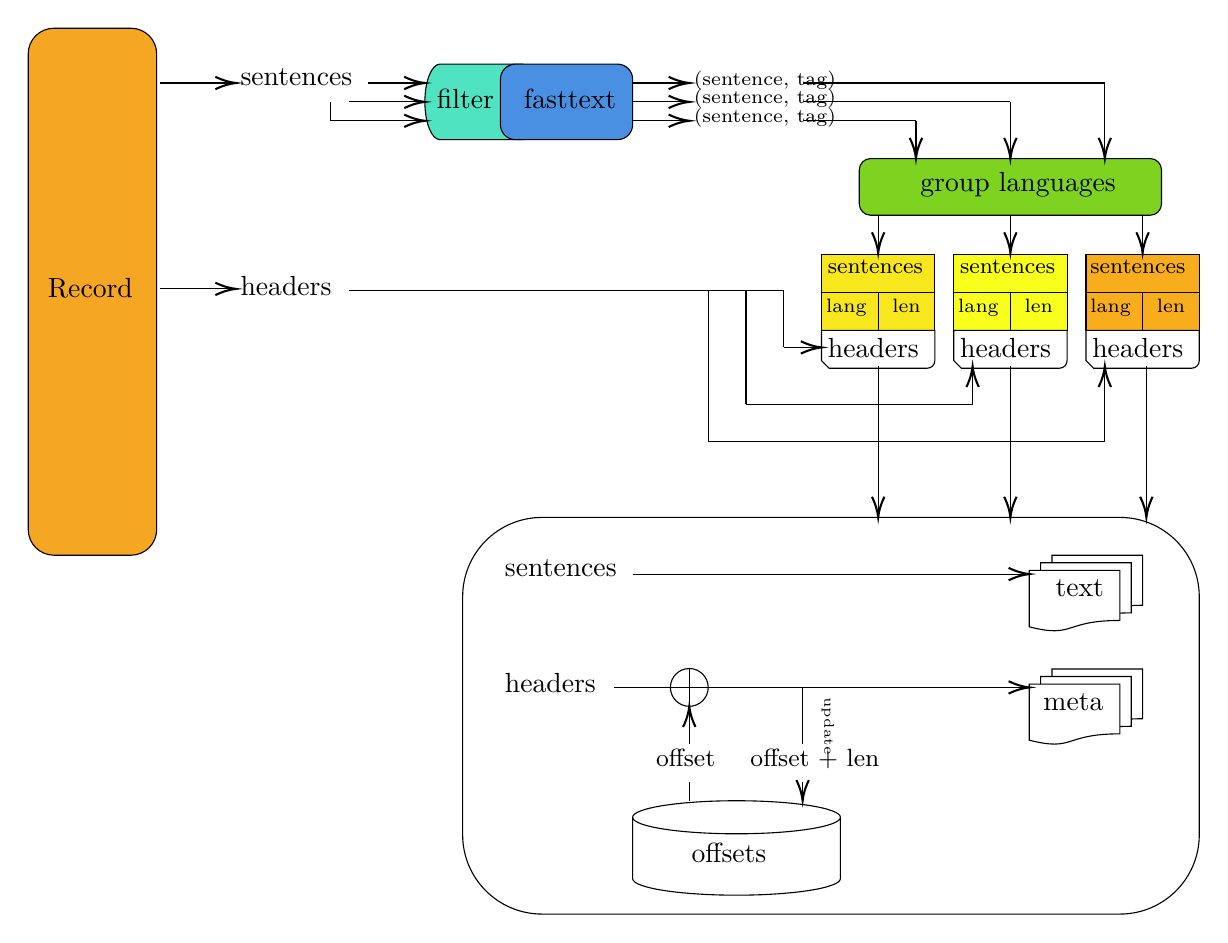
\begin{tikzpicture}[x=0.75pt,y=0.75pt,yscale=-0.91,xscale=0.91]
        %uncomment if require: \path (0,489); %set diagram left start at 0, and has height of 489

        %Flowchart: Stored Data [id:dp4699321019986179] 
        \draw  [fill={rgb, 255:red, 80; green, 227; blue, 194 }  ,fill opacity=1 ] (238,30) -- (280,30) .. controls (275.58,30) and (272,38.95) .. (272,50) .. controls (272,61.05) and (275.58,70) .. (280,70) -- (238,70) .. controls (233.58,70) and (230,61.05) .. (230,50) .. controls (230,38.95) and (233.58,30) .. (238,30) -- cycle ;
        %Rounded Rect [id:dp4628690629420654] 
        \draw  [fill={rgb, 255:red, 245; green, 166; blue, 35 }  ,fill opacity=1 ] (20,24.6) .. controls (20,17.09) and (26.09,11) .. (33.6,11) -- (74.4,11) .. controls (81.91,11) and (88,17.09) .. (88,24.6) -- (88,276.4) .. controls (88,283.91) and (81.91,290) .. (74.4,290) -- (33.6,290) .. controls (26.09,290) and (20,283.91) .. (20,276.4) -- cycle ;
        %Straight Lines [id:da8313420982420904] 
        \draw    (90,40) -- (128,40) ;
        \draw [shift={(130,40)}, rotate = 180] [color={rgb, 255:red, 0; green, 0; blue, 0 }  ][line width=0.75]    (10.93,-3.29) .. controls (6.95,-1.4) and (3.31,-0.3) .. (0,0) .. controls (3.31,0.3) and (6.95,1.4) .. (10.93,3.29)   ;
        %Straight Lines [id:da4482967760350627] 
        \draw    (90,149) -- (128,149) ;
        \draw [shift={(130,149)}, rotate = 180] [color={rgb, 255:red, 0; green, 0; blue, 0 }  ][line width=0.75]    (10.93,-3.29) .. controls (6.95,-1.4) and (3.31,-0.3) .. (0,0) .. controls (3.31,0.3) and (6.95,1.4) .. (10.93,3.29)   ;
        %Rounded Rect [id:dp9849601809689044] 
        \draw  [fill={rgb, 255:red, 74; green, 144; blue, 226 }  ,fill opacity=1 ] (270,38) .. controls (270,33.58) and (273.58,30) .. (278,30) -- (332,30) .. controls (336.42,30) and (340,33.58) .. (340,38) -- (340,62) .. controls (340,66.42) and (336.42,70) .. (332,70) -- (278,70) .. controls (273.58,70) and (270,66.42) .. (270,62) -- cycle ;

        %Straight Lines [id:da8668621904345621] 
        \draw    (200,40) -- (228,40) ;
        \draw [shift={(230,40)}, rotate = 180] [color={rgb, 255:red, 0; green, 0; blue, 0 }  ][line width=0.75]    (10.93,-3.29) .. controls (6.95,-1.4) and (3.31,-0.3) .. (0,0) .. controls (3.31,0.3) and (6.95,1.4) .. (10.93,3.29)   ;
        %Straight Lines [id:da996242982187254] 
        \draw    (180,50) -- (180,60) ;
        %Straight Lines [id:da7644452497572334] 
        \draw    (190,50) -- (228,50) ;
        \draw [shift={(230,50)}, rotate = 180] [color={rgb, 255:red, 0; green, 0; blue, 0 }  ][line width=0.75]    (10.93,-3.29) .. controls (6.95,-1.4) and (3.31,-0.3) .. (0,0) .. controls (3.31,0.3) and (6.95,1.4) .. (10.93,3.29)   ;
        %Straight Lines [id:da8688952100791735] 
        \draw    (180,60) -- (228,60) ;
        \draw [shift={(230,60)}, rotate = 180] [color={rgb, 255:red, 0; green, 0; blue, 0 }  ][line width=0.75]    (10.93,-3.29) .. controls (6.95,-1.4) and (3.31,-0.3) .. (0,0) .. controls (3.31,0.3) and (6.95,1.4) .. (10.93,3.29)   ;
        %Straight Lines [id:da26148793342838117] 
        \draw    (340,40) -- (368,40) ;
        \draw [shift={(370,40)}, rotate = 180] [color={rgb, 255:red, 0; green, 0; blue, 0 }  ][line width=0.75]    (10.93,-3.29) .. controls (6.95,-1.4) and (3.31,-0.3) .. (0,0) .. controls (3.31,0.3) and (6.95,1.4) .. (10.93,3.29)   ;
        %Straight Lines [id:da4954783851514327] 
        \draw    (340,60) -- (368,60) ;
        \draw [shift={(370,60)}, rotate = 180] [color={rgb, 255:red, 0; green, 0; blue, 0 }  ][line width=0.75]    (10.93,-3.29) .. controls (6.95,-1.4) and (3.31,-0.3) .. (0,0) .. controls (3.31,0.3) and (6.95,1.4) .. (10.93,3.29)   ;
        %Straight Lines [id:da05936926008094867] 
        \draw    (340,50) -- (368,50) ;
        \draw [shift={(370,50)}, rotate = 180] [color={rgb, 255:red, 0; green, 0; blue, 0 }  ][line width=0.75]    (10.93,-3.29) .. controls (6.95,-1.4) and (3.31,-0.3) .. (0,0) .. controls (3.31,0.3) and (6.95,1.4) .. (10.93,3.29)   ;
        %Rounded Rect [id:dp49349855068480486] 
        \draw  [fill={rgb, 255:red, 126; green, 211; blue, 33 }  ,fill opacity=1 ] (460,86) .. controls (460,82.69) and (462.69,80) .. (466,80) -- (614,80) .. controls (617.31,80) and (620,82.69) .. (620,86) -- (620,104) .. controls (620,107.31) and (617.31,110) .. (614,110) -- (466,110) .. controls (462.69,110) and (460,107.31) .. (460,104) -- cycle ;

        %Straight Lines [id:da9110150675099965] 
        \draw    (430,40) -- (590,40) ;
        %Straight Lines [id:da9102373834436741] 
        \draw    (430,50) -- (540,50) ;
        %Straight Lines [id:da007117412031712345] 
        \draw    (430,60) -- (490,60) ;
        %Straight Lines [id:da6704245551358066] 
        \draw    (590,40) -- (590,78) ;
        \draw [shift={(590,80)}, rotate = 270] [color={rgb, 255:red, 0; green, 0; blue, 0 }  ][line width=0.75]    (10.93,-3.29) .. controls (6.95,-1.4) and (3.31,-0.3) .. (0,0) .. controls (3.31,0.3) and (6.95,1.4) .. (10.93,3.29)   ;
        %Straight Lines [id:da9774749934022594] 
        \draw    (540,50) -- (540,78) ;
        \draw [shift={(540,80)}, rotate = 270] [color={rgb, 255:red, 0; green, 0; blue, 0 }  ][line width=0.75]    (10.93,-3.29) .. controls (6.95,-1.4) and (3.31,-0.3) .. (0,0) .. controls (3.31,0.3) and (6.95,1.4) .. (10.93,3.29)   ;
        %Straight Lines [id:da9977400295475213] 
        \draw    (490,60) -- (490,78) ;
        \draw [shift={(490,80)}, rotate = 270] [color={rgb, 255:red, 0; green, 0; blue, 0 }  ][line width=0.75]    (10.93,-3.29) .. controls (6.95,-1.4) and (3.31,-0.3) .. (0,0) .. controls (3.31,0.3) and (6.95,1.4) .. (10.93,3.29)   ;
        %Shape: Rectangle [id:dp2031974452528671] 
        \draw  [fill={rgb, 255:red, 248; green, 231; blue, 28 }  ,fill opacity=1 ] (440,131) -- (500,131) -- (500,171) -- (440,171) -- cycle ;
        %Shape: Rectangle [id:dp3227217281027539] 
        \draw   (440,151) -- (470,151) -- (470,171) -- (440,171) -- cycle ;
        %Shape: Rectangle [id:dp8945259346838845] 
        \draw   (470,151) -- (500,151) -- (500,171) -- (470,171) -- cycle ;
        %Shape: Rectangle [id:dp8533666881534692] 
        \draw  [fill={rgb, 255:red, 248; green, 173; blue, 28 }  ,fill opacity=1 ] (580,131) -- (640,131) -- (640,171) -- (580,171) -- cycle ;
        %Shape: Rectangle [id:dp24559484415109678] 
        \draw   (580,151) -- (610,151) -- (610,171) -- (580,171) -- cycle ;
        %Shape: Rectangle [id:dp27135592725947755] 
        \draw   (610,151) -- (640,151) -- (640,171) -- (610,171) -- cycle ;
        %Shape: Rectangle [id:dp14887885636177012] 
        \draw  [fill={rgb, 255:red, 248; green, 255; blue, 28 }  ,fill opacity=1 ] (510,131) -- (570,131) -- (570,171) -- (510,171) -- cycle ;
        %Shape: Rectangle [id:dp6142444969447188] 
        \draw   (510,151) -- (540,151) -- (540,171) -- (510,171) -- cycle ;
        %Shape: Rectangle [id:dp3599126658761931] 
        \draw   (540,151) -- (570,151) -- (570,171) -- (540,171) -- cycle ;
        %Straight Lines [id:da6637979435067474] 
        \draw    (190,150) -- (420,150) ;
        %Straight Lines [id:da0639984733030543] 
        \draw    (420,150) -- (420,180) ;
        %Straight Lines [id:da668825270485392] 
        \draw    (420,180) -- (438,180) ;
        \draw [shift={(440,180)}, rotate = 180] [color={rgb, 255:red, 0; green, 0; blue, 0 }  ][line width=0.75]    (10.93,-3.29) .. controls (6.95,-1.4) and (3.31,-0.3) .. (0,0) .. controls (3.31,0.3) and (6.95,1.4) .. (10.93,3.29)   ;
        %Straight Lines [id:da3417800565981026] 
        \draw    (400,150) -- (400,160) ;
        %Straight Lines [id:da09888916391476721] 
        \draw    (400,160) -- (400,210) ;
        %Straight Lines [id:da6576198258261287] 
        \draw    (380,150) -- (380,230) ;
        %Straight Lines [id:da39423430620012667] 
        \draw    (400,210) -- (520,210) ;
        %Straight Lines [id:da36377145787111487] 
        \draw    (380,230) -- (590,230) ;
        %Straight Lines [id:da20949009357910353] 
        \draw    (520,210) -- (520,192) ;
        \draw [shift={(520,190)}, rotate = 450] [color={rgb, 255:red, 0; green, 0; blue, 0 }  ][line width=0.75]    (10.93,-3.29) .. controls (6.95,-1.4) and (3.31,-0.3) .. (0,0) .. controls (3.31,0.3) and (6.95,1.4) .. (10.93,3.29)   ;
        %Straight Lines [id:da9243090582667062] 
        \draw    (590,230) -- (590,192) ;
        \draw [shift={(590,190)}, rotate = 450] [color={rgb, 255:red, 0; green, 0; blue, 0 }  ][line width=0.75]    (10.93,-3.29) .. controls (6.95,-1.4) and (3.31,-0.3) .. (0,0) .. controls (3.31,0.3) and (6.95,1.4) .. (10.93,3.29)   ;
        %Snip Round Single Corner Rect [id:dp6248686818369311] 
        \draw   (500,187) .. controls (500,189.21) and (498.21,191) .. (496,191) -- (444,191) -- (440,187) -- (440,171) -- (500,171) -- cycle ;
        %Snip Round Single Corner Rect [id:dp4416079275569046] 
        \draw   (570,187) .. controls (570,189.21) and (568.21,191) .. (566,191) -- (514,191) -- (510,187) -- (510,171) -- (570,171) -- cycle ;
        %Snip Round Single Corner Rect [id:dp7248479469870895] 
        \draw   (640,187) .. controls (640,189.21) and (638.21,191) .. (636,191) -- (584,191) -- (580,187) -- (580,171) -- (640,171) -- cycle ;
        %Straight Lines [id:da02360656408875572] 
        \draw    (540,110) -- (540,128) ;
        \draw [shift={(540,130)}, rotate = 270] [color={rgb, 255:red, 0; green, 0; blue, 0 }  ][line width=0.75]    (10.93,-3.29) .. controls (6.95,-1.4) and (3.31,-0.3) .. (0,0) .. controls (3.31,0.3) and (6.95,1.4) .. (10.93,3.29)   ;
        %Straight Lines [id:da5151329005041937] 
        \draw    (610,110) -- (610,128) ;
        \draw [shift={(610,130)}, rotate = 270] [color={rgb, 255:red, 0; green, 0; blue, 0 }  ][line width=0.75]    (10.93,-3.29) .. controls (6.95,-1.4) and (3.31,-0.3) .. (0,0) .. controls (3.31,0.3) and (6.95,1.4) .. (10.93,3.29)   ;
        %Straight Lines [id:da5710017720882605] 
        \draw    (470,110) -- (470,128) ;
        \draw [shift={(470,130)}, rotate = 270] [color={rgb, 255:red, 0; green, 0; blue, 0 }  ][line width=0.75]    (10.93,-3.29) .. controls (6.95,-1.4) and (3.31,-0.3) .. (0,0) .. controls (3.31,0.3) and (6.95,1.4) .. (10.93,3.29)   ;
        %Rounded Rect [id:dp34777737838988] 
        \draw   (250,312) .. controls (250,288.8) and (268.8,270) .. (292,270) -- (598,270) .. controls (621.2,270) and (640,288.8) .. (640,312) -- (640,438) .. controls (640,461.2) and (621.2,480) .. (598,480) -- (292,480) .. controls (268.8,480) and (250,461.2) .. (250,438) -- cycle ;
        %Flowchart: Multidocument [id:dp38628004470840416] 
        \draw  [fill={rgb, 255:red, 255; green, 255; blue, 255 }  ,fill opacity=1 ] (562,290) -- (610,290) -- (610,316.51) .. controls (580,316.51) and (586,326.07) .. (562,319.88) -- cycle ; \draw  [fill={rgb, 255:red, 255; green, 255; blue, 255 }  ,fill opacity=1 ] (556,294.02) -- (604,294.02) -- (604,320.53) .. controls (574,320.53) and (580,330.09) .. (556,323.9) -- cycle ; \draw  [fill={rgb, 255:red, 255; green, 255; blue, 255 }  ,fill opacity=1 ] (550,298.03) -- (598,298.03) -- (598,324.54) .. controls (568,324.54) and (574,334.1) .. (550,327.92) -- cycle ;

        %Flowchart: Multidocument [id:dp29609362181778487] 
        \draw  [fill={rgb, 255:red, 255; green, 255; blue, 255 }  ,fill opacity=1 ] (562,350.25) -- (610,350.25) -- (610,376.59) .. controls (580,376.59) and (586,386.09) .. (562,379.95) -- cycle ; \draw  [fill={rgb, 255:red, 255; green, 255; blue, 255 }  ,fill opacity=1 ] (556,354.24) -- (604,354.24) -- (604,380.58) .. controls (574,380.58) and (580,390.09) .. (556,383.94) -- cycle ; \draw  [fill={rgb, 255:red, 255; green, 255; blue, 255 }  ,fill opacity=1 ] (550,358.23) -- (598,358.23) -- (598,384.58) .. controls (568,384.58) and (574,394.08) .. (550,387.93) -- cycle ;

        %Straight Lines [id:da0033612499475468294] 
        \draw    (470,190) -- (470,268) ;
        \draw [shift={(470,270)}, rotate = 270] [color={rgb, 255:red, 0; green, 0; blue, 0 }  ][line width=0.75]    (10.93,-3.29) .. controls (6.95,-1.4) and (3.31,-0.3) .. (0,0) .. controls (3.31,0.3) and (6.95,1.4) .. (10.93,3.29)   ;
        %Straight Lines [id:da08266362916000991] 
        \draw    (540,190) -- (540,268) ;
        \draw [shift={(540,270)}, rotate = 270] [color={rgb, 255:red, 0; green, 0; blue, 0 }  ][line width=0.75]    (10.93,-3.29) .. controls (6.95,-1.4) and (3.31,-0.3) .. (0,0) .. controls (3.31,0.3) and (6.95,1.4) .. (10.93,3.29)   ;
        %Straight Lines [id:da7915660415727729] 
        \draw    (612,190) -- (612,268) ;
        \draw [shift={(612,270)}, rotate = 270] [color={rgb, 255:red, 0; green, 0; blue, 0 }  ][line width=0.75]    (10.93,-3.29) .. controls (6.95,-1.4) and (3.31,-0.3) .. (0,0) .. controls (3.31,0.3) and (6.95,1.4) .. (10.93,3.29)   ;
        %Flowchart: Magnetic Disk [id:dp4806528931350428] 
        \draw   (450,428.75) -- (450,461.25) .. controls (450,466.08) and (425.38,470) .. (395,470) .. controls (364.62,470) and (340,466.08) .. (340,461.25) -- (340,428.75)(450,428.75) .. controls (450,433.58) and (425.38,437.5) .. (395,437.5) .. controls (364.62,437.5) and (340,433.58) .. (340,428.75) .. controls (340,423.92) and (364.62,420) .. (395,420) .. controls (425.38,420) and (450,423.92) .. (450,428.75) -- cycle ;

        %Straight Lines [id:da24403954969455177] 
        \draw    (340,300) -- (548,300) ;
        \draw [shift={(550,300)}, rotate = 180] [color={rgb, 255:red, 0; green, 0; blue, 0 }  ][line width=0.75]    (10.93,-3.29) .. controls (6.95,-1.4) and (3.31,-0.3) .. (0,0) .. controls (3.31,0.3) and (6.95,1.4) .. (10.93,3.29)   ;
        %Straight Lines [id:da4710037635075677] 
        \draw    (370,420) -- (370,410) ;
        \draw   (360,360) .. controls (360,354.48) and (364.48,350) .. (370,350) .. controls (375.52,350) and (380,354.48) .. (380,360) .. controls (380,365.52) and (375.52,370) .. (370,370) .. controls (364.48,370) and (360,365.52) .. (360,360) -- cycle ; \draw   (360,360) -- (380,360) ; \draw   (370,350) -- (370,370) ;
        %Straight Lines [id:da8378723284680856] 
        \draw    (330,360) -- (360,360) ;
        %Straight Lines [id:da16198507756193636] 
        \draw    (380,360) -- (548,360) ;
        \draw [shift={(550,360)}, rotate = 180] [color={rgb, 255:red, 0; green, 0; blue, 0 }  ][line width=0.75]    (10.93,-3.29) .. controls (6.95,-1.4) and (3.31,-0.3) .. (0,0) .. controls (3.31,0.3) and (6.95,1.4) .. (10.93,3.29)   ;
        %Straight Lines [id:da13573094047430956] 
        \draw    (370,390) -- (370,372) ;
        \draw [shift={(370,370)}, rotate = 450] [color={rgb, 255:red, 0; green, 0; blue, 0 }  ][line width=0.75]    (10.93,-3.29) .. controls (6.95,-1.4) and (3.31,-0.3) .. (0,0) .. controls (3.31,0.3) and (6.95,1.4) .. (10.93,3.29)   ;
        %Straight Lines [id:da8677494244961229] 
        \draw    (430,410) -- (430,418) ;
        \draw [shift={(430,420)}, rotate = 270] [color={rgb, 255:red, 0; green, 0; blue, 0 }  ][line width=0.75]    (10.93,-3.29) .. controls (6.95,-1.4) and (3.31,-0.3) .. (0,0) .. controls (3.31,0.3) and (6.95,1.4) .. (10.93,3.29)   ;
        %Straight Lines [id:da5717074508020997] 
        \draw    (430,390) -- (430,360) ;

        % Text Node
        \draw (29,142) node [anchor=north west][inner sep=0.75pt]   [align=left] {Record};
        % Text Node
        \draw (131,31) node [anchor=north west][inner sep=0.75pt]   [align=left] {sentences};
        % Text Node
        \draw (131,141) node [anchor=north west][inner sep=0.75pt]   [align=left] {headers};
        % Text Node
        \draw (281,42) node [anchor=north west][inner sep=0.75pt]   [align=left] {fasttext};
        % Text Node
        \draw (371,32) node [anchor=north west][inner sep=0.75pt]  [font=\footnotesize] [align=left] {{\scriptsize (sentence, tag)}};
        % Text Node
        \draw (371,42) node [anchor=north west][inner sep=0.75pt]  [font=\footnotesize] [align=left] {{\scriptsize (sentence, tag)}};
        % Text Node
        \draw (371,52) node [anchor=north west][inner sep=0.75pt]  [font=\footnotesize] [align=left] {{\scriptsize (sentence, tag)}};
        % Text Node
        \draw (235,42) node [anchor=north west][inner sep=0.75pt]   [align=left] {filter};
        % Text Node
        \draw (485,86.13) node [anchor=north west][inner sep=0.75pt]   [align=left] {\begin{minipage}[lt]{78.78pt}\setlength\topsep{0pt}
                \begin{center}
                    group languages
                \end{center}

            \end{minipage}};
        % Text Node
        \draw (442,174) node [anchor=north west][inner sep=0.75pt]   [align=left] {headers};
        % Text Node
        \draw (512,174) node [anchor=north west][inner sep=0.75pt]   [align=left] {headers};
        % Text Node
        \draw (582,174) node [anchor=north west][inner sep=0.75pt]   [align=left] {headers};
        % Text Node
        \draw (442,132) node [anchor=north west][inner sep=0.75pt]   [align=left] {{\footnotesize sentences}};
        % Text Node
        \draw (441,153) node [anchor=north west][inner sep=0.75pt]   [align=left] {{\scriptsize {\fontfamily{pcr}\selectfont lang}}};
        % Text Node
        \draw (462,153) node [anchor=north west][inner sep=0.75pt]   [align=left] {\begin{minipage}[lt]{19.86pt}\setlength\topsep{0pt}
                \begin{flushright}
                    {\scriptsize {\fontfamily{pcr}\selectfont len}}
                \end{flushright}

            \end{minipage}};
        % Text Node
        \draw (511,153) node [anchor=north west][inner sep=0.75pt]   [align=left] {{\scriptsize {\fontfamily{pcr}\selectfont lang}}};
        % Text Node
        \draw (532,153) node [anchor=north west][inner sep=0.75pt]   [align=left] {\begin{minipage}[lt]{19.86pt}\setlength\topsep{0pt}
                \begin{flushright}
                    {\scriptsize {\fontfamily{pcr}\selectfont len}}
                \end{flushright}

            \end{minipage}};
        % Text Node
        \draw (581,153) node [anchor=north west][inner sep=0.75pt]   [align=left] {{\scriptsize {\fontfamily{pcr}\selectfont lang}}};
        % Text Node
        \draw (602,153) node [anchor=north west][inner sep=0.75pt]   [align=left] {\begin{minipage}[lt]{19.86pt}\setlength\topsep{0pt}
                \begin{flushright}
                    {\scriptsize {\fontfamily{pcr}\selectfont len}}
                \end{flushright}

            \end{minipage}};
        % Text Node
        \draw (512,132) node [anchor=north west][inner sep=0.75pt]   [align=left] {{\footnotesize sentences}};
        % Text Node
        \draw (581,132) node [anchor=north west][inner sep=0.75pt]   [align=left] {{\footnotesize sentences}};
        % Text Node
        \draw (369.8,441) node [anchor=north west][inner sep=0.75pt]   [align=left] {offsets};
        % Text Node
        \draw (556.13,362.04) node [anchor=north west][inner sep=0.75pt]   [align=left] {meta};
        % Text Node
        \draw (562.5,301.25) node [anchor=north west][inner sep=0.75pt]   [align=left] {text};
        % Text Node
        \draw (271,291) node [anchor=north west][inner sep=0.75pt]   [align=left] {sentences};
        % Text Node
        \draw (271,351) node [anchor=north west][inner sep=0.75pt]   [align=left] {headers};
        % Text Node
        \draw (351,391) node [anchor=north west][inner sep=0.75pt]   [align=left] {{\small offset}};
        % Text Node
        \draw (401,391) node [anchor=north west][inner sep=0.75pt]   [align=left] {{\small offset + len}};
        % Text Node
        \draw (448,364) node [anchor=north west][inner sep=0.75pt]  [rotate=-90] [align=left] {{\tiny update}};


    \end{tikzpicture}

    \caption{Record processing with metadata extraction. Headers are kept aside while sentences are identified and grouped into same-language bins. Headers are then cloned for each bin, and are sequentially stamped with an offset that is recorded for the whole operation, and written to disk into text and metadata files by language.}
    \label{fig:zoomed}
\end{figure*}

Having paragraphs and metadata linked by offsets in a highly parallelized pipeline implies to take special care at the offset level.
The solution is to use shard-scoped offsets (starting from $0$ for each language), and to keep global offsets protected by a mutex guard. This way, when a given shard is done processing and is ready to be written on disk, we convert shard-scoped offsets to global-scoped ones, update the global-scoped ones and then write text and metadata on disk.

\begin{table}[t]
    \centering\small
    \scalebox{0.85}{
        \begin{tabular}{lrrrr}
            \toprule
            Platform                 & \#shards & OSCAR & With Metadata & Speedup     \\
            \midrule
            \multirow{3}{*}{Desktop} & 1        & 13s   & 12s           & $\times$1.1 \\
                                     & 10       & 2m12s & 1m55s         & $\times$1.1 \\
                                     & 25       & 5m47s & 4m50s         & $\times$1.2 \\
            \midrule
            \multirow{3}{*}{HPC}     & 1        & 6s    & 7s            & $\times$0.9 \\
                                     & 25       & 1m6s  & 1m12s         & $\times$0.9 \\
                                     & 100      & 4m14s & 4m36s         & $\times$0.9 \\
            \bottomrule
        \end{tabular}
    }
    \caption{Comparison of approximate generation times with and without metadata generation.}
    \label{tab:pipelines-bench}
\end{table}

We compare running times for the reimplementation of the goclassy pipeline, and our new pipeline adding metadata extraction, using both desktop and HPC contexts. The results are reported in Table ~\ref{tab:pipelines-bench}.

Metadata generation does not seem to influence generation time dramatically. However, we can notice a slight performance difference between HPC and Desktop contexts. These differences may lie in the storage medium differences, I/O layout, or algorithmic peculiarities benefiting desktop contexts because of other bottlenecks.


\subsection{Characteristics of our new backward compatible OSCAR-like corpus}

We evaluate the newly generated corpus, assessing its ability to reflect events that occurred after the publication of OSCAR 2018 and detail the metadata format and potential use.

\subsubsection{Comparison with OSCAR}

While it is expected that our new corpus has a larger file size than OSCAR since CommonCrawl itself grew from 7.42TB to 8.06TB, metadata quickly adds up and take for nearly 15\% of the whole uncompressed data.

\begin{table}[t]
    \centering\small
    \scalebox{0.82}{
        \begin{tabular}{lrrrr}
            \toprule
            Version & Source & Textual (dedup) & Metadata & Total (increase) \\
            \midrule
            2018    & 7.42TB & 6.3TB (3.2TB)   & N/A      & 6.3TB            \\
            \midrule
            2021    & 8.06TB & 7.2TB (3.3TB)   & 1.2TB    & 8.4TB ($+33\%$)  \\
            \bottomrule
        \end{tabular}
    }
    \caption{Comparison of CommonCrawl and OSCAR sizes between 2018 and 2021 versions. Compressed (CommonCrawl) sources are from November 2018 and February 2021. Total is Textual + Metadata without deduplication.}
    \label{tab:oscar-size}
\end{table}

The size augmentation is not the same for each language, and while the whole corpus is bigger now, some languages are smaller than they were before.

\begin{figure}[ht]
    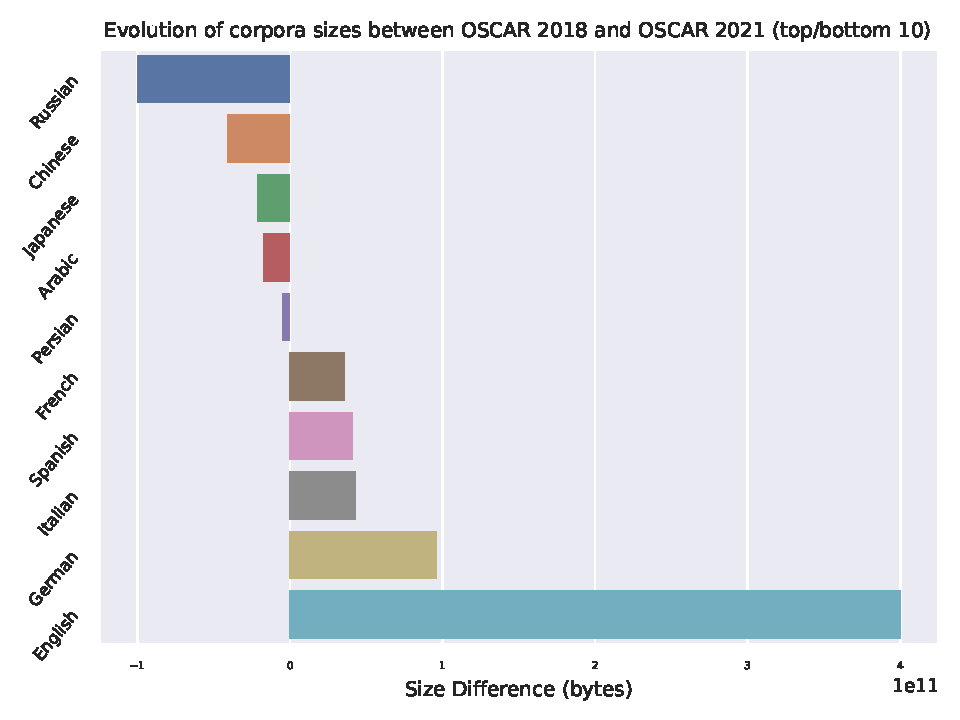
\includegraphics[width=0.48\textwidth, angle=0]{static/media/data/ungoliant/size_evo}
    \caption{Comparison of language size (in bytes) between OSCAR 2018 and OSCAR 2021 (top/bottom 5 only). }
    \label{fig:lang-size}
\end{figure}

Results show that already largely represented languages gain more and more data (like the English language, which constitutes more than a third of the original OSCAR), except for the Russian language which loses approximately 100Gb of textual content. These results are summarized in Figure~\ref{fig:lang-size}.

However, in a context where the number of languages is very high (higher than 150) and of varying sizes, evolution can't be analyzed via a mere size evaluation. By computing, for each language, the relative size difference between the 2018 and 2021 releases of OSCAR, less resourced languages do appear, hinting at a better representation of some of them. These results can be found in Figure~\ref{fig:lang-size-pctg}.

Numerous languages have been omitted from Figure~\ref{fig:lang-size-pctg}, either:
\begin{itemize}
    \item because they were present in the original OSCAR and are now absent (\textit{Central Bikol} and \textit{Cantonese})
    \item because they were absent in the original OSCAR and are now present (\textit{Manx}, \textit{Rusyn}, \textit{Scots} and \textit{West Flemish})
\end{itemize}

Precautions have to be taken when using these corpora and further work has to be done to correctly assess the quality of low-to-mid resource languages in order to better reflect the quality of each corpus to the OSCAR users. Some languages exhibited either a particularly low number of sentences or a very low quality, and as such couldn't be usable, while still accounting for a language in the total language count of the original OSCAR.

\begin{figure}[ht]
    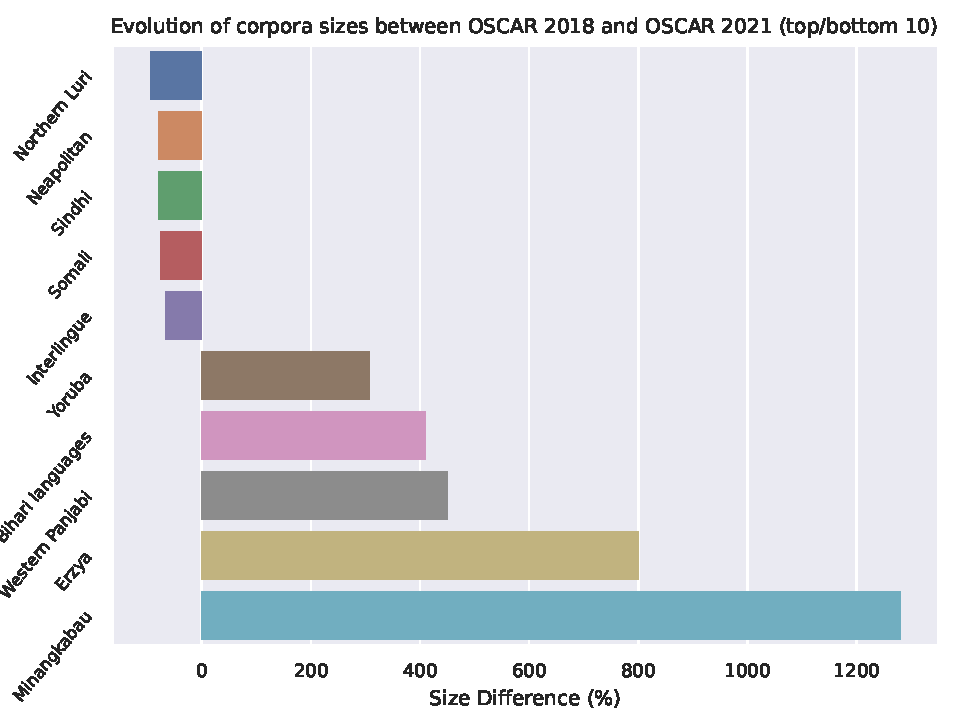
\includegraphics[width=0.48\textwidth, angle=0]{static/media/data/ungoliant/size_evo_pctg}
    \caption{Comparison of language percentage between OSCAR 2018 and OSCAR 2021 (top/bottom 5 only).}
    \label{fig:lang-size-pctg}
\end{figure}

\subsubsection{Metadata}

Metadata provides new contextual data that is useful to evaluate the corpus and draw metrics.

The total size of metadata is 1.2TB, ranging from 4Kb to 500Gb, depending on the number of lines.
Relative size varies from 100\% to 20\%, diminishing with the textual data size, which is expected.

Metadata are provided in single files for now, but split versions of both textual and contextual data will be released soon after the release of the corpus, enabling easy access.

Our choice of keeping metadata aside from the main content adds some complexity when working with both textual and contextual data:

\begin{itemize}
    \item When trying to get the metadata of given sentence, one has to get the line number $k$, then sequentially (or use a search algorithm since offsets are sorted) look for the record (with offset $o$ and length $l$), where $k \in [o, o+l]$.
    \item Looking for lines corresponding to a particular metadata entry is easier: one has to read the textual file, skipping until the $o$-th line, then read $l$ lines.

\end{itemize}


\subsubsection{Presence of events}

Using a sample of an English part of our corpus, we perform a simple search of terms in order to assess and compare the presence of pre- and post- 2018 events and persons in both corpora. Terms and frequency are grouped in Table \ref{tab:word-frequency}.

\begin{table}[t]
    \centering\small
    \begin{tabular}{lrrrr}
        \toprule
        Language                  & Term                  & 2018  & 2021  \\
        \midrule
        \multirow{1}{*}{Arabic}   & Beirut port explosion & 0     & 31    \\
        \multirow{1}{*}{Burmese*} & Min Aung Hlaing       & 387   & 3439  \\
        \multirow{1}{*}{English}  & Obama                 & 30039 & 27639 \\
        \multirow{1}{*}{English}  & Biden                 & 990   & 19299 \\
        \multirow{1}{*}{French}   & Yellow Vests          & 2     & 96    \\
        \bottomrule
    \end{tabular}
    \caption{Comparison of occurrences of news-related terms between OSCAR and our corpus in a sample of 100 CommonCrawl shards. For the Burmese language, we use the whole 2018 and 2021 corpus since it is a low resource language. Terms are translated in the corpus language.}
    \label{tab:word-frequency}
\end{table}

Our corpus keeps around the same number of occurrences for pre-2018 events or public figures such as Barack Obama, while increasing the occurrence of people linked to more recent events (Joe Biden).

We include search terms linked to post-2018 events in French and Arabic which are smaller corpora (resp. 200 and 80 GB), and in Burmese, a mid-resource language (approximately 2GB). We observe a term occurrences evolution that reflects the linked events' timing and importance.

\subsection{License}

This new corpus will be released under a research-only license that is compliant with the EU's exceptions for research in text and data mining. Contrarily to the original OSCAR, no shuffled version of the corpus will be distributed, instead we will put in place an authentication system that will allow us to verify that requests for the corpus come from research institutions. A contact form will be also provided for independent researchers so that we can study their particular cases and determine if the utilization of the corpus corresponds to a legitimate research use.

Moreover, the introduction of metadata makes our corpus far more queryable, thus simplifying and speeding up the handling of take-down GDPR requests. For this reason, we will be releasing the complete set of metadata under a CC0 public domain license, so that any individual can check if their personal or even copyrighted data is in our new corpus and make a request accordingly.

\section{Conclusion}

We show that our solution is able to generate an OSCAR-like corpus that is augmented with metadata without breaking compatibility, while being faster, better tested and thoroughly documented. We believe our new pipeline and corpus will be useful for applications in computational linguistics as well as in corpus linguistics in general.

The generated corpus is of a larger size when including metadata and without deduplication. However, deduplicated textual content is of the same magnitude between OSCAR 2018 and OSCAR 2021, while reflecting topic changes from all over the world. This fact suggests that old data may be lost with the time passing, and could be resolved by using CommonCrawl releases to build an incremental corpus, with every version augmenting the corpus size.

Metadata enables queries and statistics on the generated data, and we believe that it can be used to filter OSCAR to generate corpora that respond to certain criteria.

We plan to make this new version of OSCAR available under research constraints, with split versions of both textual content and metadata along with tools to operate on the corpus, enabling fast and easy operation on the corpus for researchers.
\chapter{CaBeRnet}

\section{Introduction}\label{sect:Intro}

The question of quality versus size of training corpora is increasingly gaining attention and interest in the context of the latest developments in neural language models' performance.
The longstanding issue of corpora "representativeness" is here addressed, in order to grasp to what extent a linguistically balanced cross-genre language sample is sufficient for a language model to gain in accuracy for contextualized word-embeddings on different NLP tasks.

Several increasingly larger corpora are nowadays compiled from the web, i.e. frWAC \citep{baroni-etal-2009-the}, CCNet \citep{wenzek-etal-2020-ccnet} and OSCAR-fr \citep{ortiz-suarez-etal-2019-asynchronous}. However, does large size necessarily go along with better performance for language model training? Their alleged lack of representativeness has called for inventive ways of building a French balanced corpus offering new insights into language variation and NLP.

Following Biber's definition, “representativeness refers to the extent to which a sample includes the full range of variability in a population” \citep{biber-1993-representativeness}. We adopt a balanced approach by sampling a wide spectrum of language use and its cross-genre variability, be it situational (e.g.\ format, author, addressee, purposes, settings or topics) or linguistic, e.g.\ linked to distributional parameters like frequencies of word classes and genres.
In this way, we developed two newly built corpora. The French Balanced Reference Corpus - \textit{CaBeRnet} - includes a wide-ranging and balanced coverage of cross-genre language use to be maximally representative of French language and therefore yield good generalizations from. The second corpus, the \textit{French Children Book Test} (CBT-fr), includes both narrative material and oral language use as present in youth literature, and will be used for domain-specific language model training. Both are inspired by existing American and English corpora, respectively  COCA, the balanced Corpus of Contemporary American English \citep{davies-2009-the, davies-2010-the}, and the Children Book Test \citep[CBT]{hill-etal-2016-the}.

%better performing word-embeddings
%evaluate the quality of word embedding generated by pre-training 
The second main contribution of this paper lies in the evaluation of the quality of the word-embeddings obtained by pre-training and fine-tuning on different corpora, that are made here publicly available.
Based on the underlying assumption that a linguistically representative corpus would possibly generate better word-embeddings. %being more representative of real language use, would tentatively preform better in downstream tasks. 
We provide an evaluation-based investigation of how a balanced cross-genre corpus can yield improvements in the performance of neural language models like ELMo \citep{peters-etal-2018-deep} on various downstream tasks.
The two corpora, \Cabernet and CBT-fr, and the ELMos will be distributed freely under Creative Commons License.

Specifically, we want to investigate the contribution of oral language use as present in different corpora. Through a series of comparisons, we contrast a more domain-specific and written corpus like Wikipedia-fr with the newly built domain-specific CBT-fr corpus which additionally features oral style dialogues, like the ones one can find in youth literature. To test for the effect of corpus size, we further compare a wide ranging corpora characterized by a variety of linguistic phenomena crawled from internet, like OSCAR \citep{ortiz-suarez-etal-2019-asynchronous}, with our newly built French Balanced Reference Corpus \Cabernet.
Our aim is assess the benefits that can be gained from a balanced, multi-domain corpus such as \Cabernet, despite its being 34 times smaller than the web-based OSCAR.

%Methodologically, our approach constitutes an original proof-of-concept that fine-tuning with resources that are up to 35 times smaller than pre-training corpora has a observable impact on classical NLP tasks scores. Secondly, we show that pre-training a language model on a very small sample like the French Children Book Test corpus yields unexpected positive results.
%\iffalse
%Resources associated to this paper encompass\footnote{The link to the corpus and FrElMos will be available upon acceptance of the paper. Following the link the reader will have access to a dedicated website \textit{cabernet-corpus.fr} where raw text version and metadata for each sub-part of the corpus are also be available.} five version of FrELMo trained on the four corpora presented in this paper and two newly brewed corpora - The French Balanced Reference Corpus CaBeRnet and the French Children Book Test.
%\fi

%In sum, this paper offers three main contributions: (1) two newly built corpora one French Balanced Reference Corpus and a second domain-specific corpus having both oral and written style, (2) five versions of FrELMo, and (3) a whole array of computational results that deepen our understanding on the effects of balance and register in NLP evaluation. 


%The data for corpus creation has been extracted from selected sections of open data including dumped data from the web and section of already published corpora that specialize on a given register of source.


%%%%%%%%%%%%%%%%%%%%%%%%%%%%%%%%%%%%%%%%%%%%%%%%%%%%%%%%%
%\subsection{The present Paper}\label{ssect:Paper_struct}

%The paper presents two substantially different training corpora, proposing a set of evaluations to enquire on the accuracy of Language Models

%We report a few experiments designed to better understand the computational impact of the quality and size of training corpora with the method and tasks described so far. All the experiments are performed on xxx.

%Crucially, manipulating the presence of oral transcriptions and oral based text will be interesting to understand the impact on accuracy of our language model and their impact on several language tasks after fine-tuning. 

%\paragraph{Structure of the paper}
The paper is organized as follows. Sections \ref{sec:DescribeCorpora} and \ref{sec:CompareCorpora} are dedicated to a descriptive overlook of the building of our two newly brewed corpora \Cabernet and CBT-fr, including quantitative measures like type-token ratio and morphological richness. %corpora building and data collection. The construction process of  is here presented.% through
%in this section that summarizes information details that can be found in corpora metadata. The achievement of linguistic balance in \Cabernet is detailed in section \ref{subsec:DescribeCaBeRnet}. 
%statistics on the distribution of lexical, syntactic and morphological features of the different sub-parts of the corpus are also presented. 
%Section \ref{sec:CompareCorpora} focuses on several quantitative measures characterizing the corpora under comparison : number of sentences, type-token ratio and morphological richness. %The characteristics of CBT-fr and \Cabernet are compared to the other corpora under analysis (OSCAR-fr, Wiki-fr). 
Section \ref{sect:EvalMethod} presents the evaluation methods for POS-tagging, NER and dependency Parsing tasks, while results are introduced in §\ref{sect:ResultsCorpora}
Finally, we conclude in §\ref{sec:Concl} on the computational relevance of word-embeddings obtained through a balanced and representative corpus, and broaden the discussion on the benefits of smaller and noiseless corpora in neural NLP.% and some future developments of \Cabernet.

%\notemumu{@ALL should we say here why each corpus ? and summarize the table here under \ref{Table_copus_feature} commented here under}

%\begin{table}[htbp]
%\centering
%\begin{tabular}{lccccc}\\\toprule
%Corpora     & noise     & Range     & O/W    & Ling. \\\midrule
%OSCAR-fr    &  -        &   +      &  -      &   -    \\%\midrule 
%\Cabernet   &  +        &   +      &  both   &   +     \\%\midrule 
%Wiki-fr     &  +        &   -      &  -      &   -    \\%\midrule 
%CBT-fr      &  +        &   -      &  both   &   -     \\\bottomrule  
%\end{tabular}
%\caption{\label{Table_copus_feature} Comparison of corpora. Full-fledged linguistic representativity.}
%\end{table}


%%%%%%%%%%%%%%%%%%%%%%%%%%%%%%%%%%%%%%%%%%%%%%%%%%%%%%%%%%%%%%%%%%%
%%%%%%%%%%%%%%%%%%%%%%% A-  corpus Description.    %%%%%%%%%%%%%%%%
%%%%%%%%%%%%%%%%%%%%%%%%%%%%%%%%%%%%%%%%%%%%%%%%%%%%%%%%%%%%%%%%%%%

\section{Corpora Building}%- Quantitative Description
\label{sec:DescribeCorpora}
%Two main criteria guided corpus building, the first was balance and representativeness, and the second was maximizing the usage of open resources to build our corpora.

\subsection{\Cabernet} \label{subsec:DescribeCaBeRnet}

\Cabernet corpus was inspired by the genre partition of the American balanced corpus COCA, %\footnote{\url{https://www.corpusdata.org}}
which currently contains over 618 million words of text (20 million words each year 1990-2019) and is equally divided among spoken, fiction, popular magazines, newspapers, and academic texts \citep{davies-2009-the, davies-2010-the}. A second reference, guiding our approach and sampling method, is one of the earliest precursors of balanced reference corpora: the BNC \citep{bnc-2007-the}, first covered a wide variety of genres, with the intention to be a representative sample of spoken and written language.

\Cabernet was obtained by compiling existing data-sets and web-text extracted from different sources as detailed in this section. As shown in Table \ref{Table_Morpho_CabernetSub}, genres sources are evenly divided ($\sim$120 million words each) into spoken, fiction, magazine, newspaper, academic to achieve genre-balanced between oral and written modality in newspapers or popular written style, technical reports and Wikipedia entries, fiction, literature or academic production).
%(cf. Metadata)
%Encompassing five different genres and registers : xxx

\paragraph{\Cabernet Oral} \label{subsec:DescribeCaBeRnetOral}
The oral sub-portion gathers both oral transcriptions (\textsc{ORFEO} and Rhapsodie\footnote{\textsc{ORFEO} corpus available at \url{www.cocoon.huma-num.fr/exist/crdo/} ; Rhapsodie corpus at \url{www.projet-rhapsodie.fr}.}) and Films subtitles (Open Subtitles.org), pruned from diacritics, interlocutors tagging and time stamps. To these transcriptions, the French European Parliament Proceedings (1996-2011), as presented in \citet{koehn-2005-europarl}, contributed a sample of more complex oral style with longer sentences and richer vocabulary.%\url{www.opensubtitles.org/fr}

\paragraph{\Cabernet Popular Press} \label{subsec:DescribeCaBeRnetPop}
The whole sub-portion of Popular Press is gathered from an open data-set from the \textit{Est  Républicain} (1999, 2002 and 2003), a regional press format\footnote{Corpus available at \url{www.cnrtl.fr/corpus/estrepublicain/}.}. %Ce corpus est constitué des données textuelles correspondant à deux années de toutes les éditions intégrales du quotidien régional.
It was selected to match popular style as it is characterized by easy-to-read press style and a wide range of every-day topics characterizing local regional press.

\paragraph{\Cabernet Fiction \& Literature} \label{subsec:DescribeCaBeRnetFic}
The Fiction \& Literature sub-portion was compiled from march 2019's Wiki Source and WikiBooks dump and extracted using WikiExtractor.py, a script that extracts and cleans text from a WikiMedia database dumps, by performing template expansion and preprocessing of template definitions.\footnote{Script available at \url{https://github.com/attardi/wikiextractor}.}

\paragraph{\Cabernet News} \label{subsec:DescribeCaBeRnetNews}
The News sub-portion builds upon web crawled elements, including Wikimedia's NewsComments and WikiNews reports from may 2019 WikiMedia dump, collected with a custom version of WikiExtractor.py.
Newspaper's content gathered by the Chambers-Rostand Corpus (i.e. Le Monde 2002-2003, La Dépèche 2002-2003, L'Humanité 2002-2003) and \textit{Le Monde diplomatique} open-source corpus were assembled to represent a higher register of written news style from different political and thematic horizons.
Several months of French Press Agency reports (AFP, 2007-2011-2012) competed with more simple and telegraphic style the newspaper written sample of the corpus.\footnote{At the time being, this part of \Cabernet corpus is still subject to Licence restrictions. This restricted amount of AFP news reports can reasonably fall in the public domain.}

\paragraph{\Cabernet Academic} \label{subsec:DescribeCaBeRnetAcad}
The academic genre was also built from different sources including technical and educational texts from WikiBooks and Wikipedia dump (prior to 2016) for their thematic variety of highly specialized written production. \textsc{ORFEO} Corpus offered a small sample of academic writings like PHD dissertations and scientific articles encompassing a wide choice of disciplinary topics, and TALN Corpus\footnote{TALN proceedings corpus (about 2 million) builds on a subset of 586 scientific articles (from 2007 to 2013), namely TALN and RECITAL. Available at \url{redac.univ-tlse2.fr/corpus/taln_en.html}.} was included to represent more concise written style characterizing scientific abstracts and proceedings.

\begin{table}[ht]
    \centering\small
        \begin{tabular}{lrrr}                                                                                      \\\toprule
            {\textsc{\Cabernet Sub-set}} & {\textsc{Tokens}} & {\textsc{Unique Forms}} & {\textsc{TTR}} \\\midrule
            Oral                         & 122 864 888       & 291 744                 & 0.0024         \\
            Popular                      & 131 444 017       & 458 521                 & 0.0035         \\
            News                         & 132 708 943       & 462 971                 & 0.0035         \\
            Fiction                      & 198 343 802       & 983 195                 & 0.0050         \\
            Academic                     & 126 431 211       & 1 433 663               & 0.0113         \\
            \textit{Total}               & 711 792 861       & 2 558 513               & 0.0036         \\ \bottomrule
        \end{tabular}
    \caption{\label{Table_Morpho_CabernetSub} Comparison of number of unique forms in the different genres represented by \Cabernet partition. TTR: Type-Token Ration. Lemmatization and tokenization was performed as described in §\ref{sec:CompareCorpora}.}
\end{table}
%%%check !! 
%\begin{table}[htbp]
%\centering
%\scalebox{0.83}{
%\begin{tabular}{lrrr}\\
%\toprule
%\multicolumn{2}{}{French Balanced Reference Corpus - \textbf{\Cabernet}}\\\midrule
%{\sc \textbf{\Cabernet}}   & nb{\sc Tokens}    & nb {\sc Unique Forms}  & Mo \\\midrule
%Oral        &  122,864,888      & 291,744  & 735,4 Mo   \\ 
%Popular     &  131,444,017      & 458,521  & 758,5 Mo   \\  
%News        &  132,708,943      & 462,971  & 797,2 Mo   \\ 
%Fiction     &  198,343,802      & 983,195  & 1 080 Mo    \\
%Academic    &  126,431,211      & 1433663  & 810,8 Mo   \\
%Tot.        &  711,792,861     & 2,558,513 & 4 190 Mo   \\ \bottomrule  
%\end{tabular}}
%\caption{\label{Table_TTR_CabernetSub} Comparison of number of unique forms in the different genres represent by \Cabernet partition into Oral, Popular, News, Fiction and Academic. Mo: Mega Octet. lemmatisation and tokenisation was achieved as described in section \ref{sec:CompareCorpora}}
%\end{table}
%voir si remplaçabl

For all sub-portions of \Cabernet, visual inspection was performed to remove section titles, redundant meta-information linked to publishing schemes of each of the six news editor includes. This was manually achieved by compiling a rich set of regular expressions specific of each textual source to obtain clean plain text as an outcome.


\subsection{French Children Book Test (CBT-fr)}
\label{subsec:DescribeCBT}

The French Children Book Test (CBT-fr) was built upon its original English version, the Children Book Test (CBT) \citet{hill-etal-2016-the}\footnote{This data-set can be found at \url{www.fb.ai/babi/}.}, which consists of books freely available on \url{www.gutenberg.org}{Project Gutenberg}.

Using youth literature and children books guarantees a clear narrative structure, and a large amount of dialogues, which enrich with oral register the literary style of this corpus.
The English version of this corpus was originally built as benchmark data-set to test how well language models capture meaning in context. It contains 108 books, and a vocabulary size of 53,628.

French version of CBT, named CBT-fr, was constructed to guarantee enough linguistic similarities between the collected books in the two languages. 104 freely available books were included. One third of the books were purposely chosen because they were classical translations of English literary classics. % (see Metadata). %www.cabernet-corpus.fr 
Chapter heads, titles, notes and all types of editorial information were removed to obtain a plain narrative text. The effort of keeping proportion, genre, domain, and time as equal as possible yields a multilingual set of comparable corpora with a similar balance and representativeness.

\begin{table}[ht]
    \centering\small
        \begin{tabular}{lr}                                                             \\\toprule
            {\textsc{Children Book Test - fr}}           & { \textsc{words}} \\\midrule
            number of different lemmas                   & 25 139            \\
            total number of forms                        & 95 058            \\
            mean number of forms per lemma               & 3.78              \\
            Number of lemmas having more than one form : & 14 128            \\
            Percentage of lemmas with multiple forms     & 56.20             \\
            \bottomrule
        \end{tabular}
    \caption{\label{Table_DescribeCBTfr} Lexical statistics of French CBT, performed as described in §\ref{sec:CompareCorpora}}
\end{table}

%%%%%%%%%%%%%%%%%%%%%%%%%%%%%%%%%%%%%%%%%%%%%%%%%%%%%%%%%%%%%%%%%%
%%%%%%%%%%%%%%%%%%%%%%      Section 3    %%%%%%%%%%%%%%%%%%%%%%%%%
%%%%%%%%%%%%%%%%%%%%%%%%%%%%%%%%%%%%%%%%%%%%%%%%%%%%%%%%%%%%%%%%%%
\section{Corpora Descriptive Comparison} \label{sec:CompareCorpora}

We used two different tokenizers: SEM, Segmenteur-Étiqueteur Markovien standalone \citet{dupont-2017-exploration} and TreeTagger. Both are based on cascades of regular expressions, and both perform tokenization and sentence splitting.
The first was used for descriptive purposes because it technically allowed to segment and tokenize all corpora including OSCAR (23 billion words). Hence, all corpora were entirely segmented into sentences and tokenized using SEM.

The second tokenization method was run only on 3 million words samples to automatically tag them with TreeTagger into part-of-speech and lemmatize them.\footnote{Based on the tag-set available at \url{https://www.cis.uni-muenchen.de/~schmid/tools/TreeTagger/data/french-tagset.html}.} All corpora were randomly shuffled by sentence to then select samples of 3 million words, to be able to compare them in terms of lexical composition (Type-Token Ratio, see Table \ref{Table_MorphoRich}).
%All corpora were POS-Tagged for descriptive reasons using MElt POS-tagging (\citep{denis2012coupling} and \citep{sagot2016external}). Vocabulary size was evaluated after Lemmatization of each Corpus with MElt tool.

\subsection{Corpora Size and Composition}
%\notemumu{@Eric est-ce que je raporte la moyenne ou la mediane ou les deux ? je me rappelle que dans tes scripts tu as les deux.}

Length of sentences is a simple measure to quantify both sentence syntactic complexity and genre. Hence, the number of sentences reported in Table \ref{Table_nb_Words} shows interesting patterns of distributions across genres, consider the comparison between \Cabernet an Wiki-fr.
In our effort to evaluate the impact of corpora pre-training on ELMo-based contextualized word-embedding, we introduce here our two terms of comparison, namely the crawled corpus OSCAR-fr and the Wikipedia-fr one.
%an average length per sentence of 
%xxx for OSCAR-fr, xxx for frWac, xxx for Wiki-fr, xxx for \Cabernet and xx for CBT-fr.
%TODO

\subsubsection{OSCAR fr}
As it has been shown that pre-trained language models can be significantly improved by using more data \citep{liu-etal-2019-roberta,raffel-etal-2020-exploring}, we decided to include in our comparison a corpus of French text extracted from Common Crawl\footnote{More information available  at \url{https://commoncrawl.org/about/}.}. We leverage on a recently published corpus, OSCAR \citep{ortiz-suarez-etal-2019-asynchronous}, which offers a pre-classified and pre-filtered version of the November 2018 Common Craw snapshot.

OSCAR gathers a set of monolingual text extracted from Common Crawl - in plain text \emph{WET} format - where all HTML tags are removed and all text encodings are converted to UTF-8. It follows a similar approach to \citep{grave-etal-2018-learning} by using a language classification model based on the fastText linear classifier \citep{joulin-etal-2016-fasttext,joulin-etal-2017-bag} pre-trained on Wikipedia, Tatoeba and SETimes, supporting 176 different languages.

After language classification, a deduplication step is performed without introducing a specialized filtering scheme: paragraphs containing 100 or more UTF-8 encoded characters are kept. This makes OSCAR an example of unfiltered data that is nearly as noisy as to the original Crawled data.%\footnote{We did not use CCNet because of its difficult availability and download.}

%\subsubsection{frWac} %on l'enlève !
%The frWaC corpus is a French text corpus collected from the .fr domain with using medium-frequency words from the Le Monde Diplomatique corpus and basic French vocabulary lists as seeds. The corpus consists of French websites with total size 1.3 billion words (xxx).%add to biblio

%%%%%%%%%%%%%%%%%%%%%%%%%%%%%%%%%%%%%%%%%%%%%%%%%
\subsubsection{FrWIKI}
This corpus collects a selection of pages from Wikipedia-fr from a dump executed in April 2019, where HTML tags and tables were removed, together with template expansion using Attardi's tool (WikiExtractor, §\ref{subsec:DescribeCaBeRnetFic}). As reported on Table \ref{Table_nb_Words}, in this data-set (660 million words) sentences are relatively longer compared to other corpora. It has the advantage of having a comparable size to \Cabernet, but its homogeneity in terms of written genre is set to Wikipedia entries descriptive style.

\begin{table}[ht]
    \centering
        \begin{tabular}{lrrr}                                                                                 \\\toprule
            {\textsc{corpus}} & { \textsc{wordforms}} & { \textsc{tokens}} & { \textsc{sentences}} \\\midrule
            OSCAR-fr          & 23 212 459 287        & 27 439 082 933     & 1 003 261 066         \\
            Wiki-fr           & 665 599 545           & 802 283 130        & 21 775 351            \\
            \Cabernet         & 697 119 013           & 830 894 133        & 54 216 010            \\
            CBT-fr            & 5 697 584             & 6 910 201          & 317 239               \\\bottomrule
            %frWac       &  1,357,598,417  & 1,622,619,337  &  57,236,199  \\  
        \end{tabular}
    \caption{\label{Table_nb_Words} Comparing the corpora under study.}
\end{table}
%%%%%%%%%%%%%%%%%%%%%%%%%%%%%%%%%%%%%%%%%%%%%%%%%%%%%%%%%%%%%%%%
%%%%%%%%%%%%%%%%%%%%%%%%%%%%%%%%%%%%%%%%%%%%%%%%%%%%%%%%%%%%%%%%
\subsection{Corpora Lexical Variety}

Focusing on a useful measure of complexity that documents lexical richness or variety in vocabulary, we present the type-token ration (TTR) of the corpora under analysis. Generally used to asses language use aspects like the variety of different words used to communicate by learners or children, it represents the total number of unique words (types/forms) divided by the total number of tokens in a given sample of language production. Hence, the closer the TTR ratio is to 1, the greater the lexical richness of the corpus. Table \ref{Table_Morpho_CabernetSub} summarizes the lexical variety of the five sub-portions of \Cabernet, respectively taken as representative of Oral, Popular, Fiction, News, and Academic genres. Domain diversity of texts can be observed in the lexical statistics showing a gradual increase in the number of distinct lexical forms (cf. TTR). This pattern  reflects a generally acknowledged distributional pattern of vocabulary-size across genres. Oral style shows a poorer lexical variety compared to newspapers/magazines’ textual typology. The lexically rich fictional/classic literature is outreached by academic writing-style with its wide-ranging specialized vocabulary. All in all, Table \ref{Table_Morpho_CabernetSub} quantitatively demonstrates that the selected textual and oral materials are indeed representative of the five types of genres of CaBeRnet.


%\textbf{DEFINITION :} The Type Token Ratio (TTR). The TTR is the number of Types divided by the number of Tokens. The closer the TTR is to 1 the more lexical variety there is. Enter Henry's TTR for his written sample in Table 1 below.


%%%%%%%%%%%%%%%%%%%%%%%%%%%%%%%%%%%%%%%%%%%%%%%%%%%%%%%%%%%%%%%%%%
%%%%%%%%%%%%%%%%%%%%%%%%%%%%%%%%%%%%%%%%%%%%%%%%%%%%%%%%%%%%%%%%%%
\subsection{Corpora Morphological richness}

To select a measure that would help quantifying the different corpora morphological richness, we follow \citep{bonami-etal-2015-implicative}. Hence, the proportion of lemmas with multiple forms in a given vocabulary size was evaluated on randomly selected samples of 3-million-words from each corpus under analysis (see Table \ref{Table_MorphoRich}).
%Distribution of the lemmas in function of the percentage of their full flexion . 

%\notemumu{@Benoit : je suis pas sûre de bien ex-primer ici le contenu de nos discussions sur le sujet}

\begin{table}[ht]
    \centering
        \begin{tabular}{lrrrr}
            \toprule
            \textsc{3 M samples}  & \textsc{CBT-fr} & \textsc{\Cabernet} & \textsc{Fr-Wiki} & \textsc{OSCAR} \\
            \midrule
            nb of diff. lemmas    & 25 139          & 30 488             & 31 385           & 31 204         \\
            tot. nb forms         & 95 058          & 180 089            & 238 121          & 190 078        \\
            mean nb forms/lemma   & 3.78            & 6.19               & 7.85             & 6.40           \\
            nb lemmas $>$ 1 form  & 14 128          & 15 927             & 15 182           & 16 480         \\
            \% lemmas  $>$ 1 form & 56.20           & 52.24              & 48.37            & 52.81          \\
            \bottomrule
        \end{tabular}
    \caption{Lexical statistics on morphological richness over randomly selected samples of 3 million words from each corpus. nb : number}
    \label{Table_MorphoRich}
\end{table}

Table 4 reports some more in-depth lexical and morphological statistics across corpora. Although OSCAR is 34 times bigger than CaBeRnet, their total number of forms and the proportion of lemmas having more than one form in a 3-million-word sample are comparable. FrWiki shows a radically different lexical distribution with numerous hapaxes but a lower morphological richness. Although its total number of forms is more than one third higher than in OSCAR and CaBeRnet samples, the proportion of lemmas having more than one distinct form is around four points below CaBeRnet and OSCAR. Comparatively, youth literature in CBT-fr shows the greatest morphological richness, around 56\% of lemmas have more than one form.

%\begin{table}[ht]
%\centering\small
%\scalebox{0.95}{
%\begin{tabular}{lr}\\\toprule

%{\sc CBT-fr 3 m sample}   &   \\\midrule

%%%number of different lemmas    & 25.139   \\ 
%%total number of forms       &  95.058  \\  
%%mean number of forms per lemma     &  3,78   \\ 
%%Number of lemmas having more than one form :   &  14.128  \\
%%Percentage of lemmas with multiple forms  &  56,20 %\\\midrule

% CBT-fr
%number of forms: 70230
%number of lemmas: 22123
%mean number of forms per lemma: 74819 3.381955430999412
%proportion of lemmas with multiple forms: 11808 0.5337431632237942

%%{\sc CaBeRnetFRanc 3 m sample}   &   \\\midrule
%%number of different lemmas          & 30 488   \\ 
%%total number of forms               &  180.089  \\  
%%mean number of forms per lemma      &  6,19   \\ %188.675
%%Number of lemmas having more than one form :   &  15.927  \\
%%Percentage of lemmas with multiple forms  & 52,24 %\\\midrule

%CaBeRnetFRanc.txt
%number of forms: 
%number of lemmas: 30488
%mean number of forms per lemma: 188675 6.188500393597481
%proportion of lemmas with multiple forms: 15927 0.5224 022566255576

%{\sc frWAC 3 m sample}   &   \\\midrule
%number of different lemmas    & 30.892   \\ 
%total number of forms       &  194.562  \\  
%mean number of forms per lemma     &  6,62 \\ 
%Number of lemmas having more than one form :   &  16.197  \\
%Proportion of lemmas with multiple forms  &  52,43 \\\midrule
% frwac
%number of forms: 194562
%number of lemmas: 30892
%mean number of forms per lemma: 204400 6.61659976692995
%proportion of lemmas with multiple forms: 16197 0.5243 105011006086

%%{\sc frwiki 3 m sample}   &   \\\midrule
%%number of different lemmas    & 31.385   \\ 
%%total number of forms       &  238.121  \\  
%%mean number of forms per lemma     &  7,85   \\ 
%Number of lemmas having more than one form :   &  15.182  \\
%%Percentage of lemmas with multiple forms  &  48,37 %\\\midrule
% frwiki
%number of forms: 238121
%number of lemmas: 31385
%mean number of forms per lemma: 246418 7.851457702724232
%proportion of lemmas with multiple forms: 15182 0.4837 3426796240243

%{\sc OSCAR 3 m sample}   &   \\\midrule
%number of different lemmas    & 31.204   \\ 
%%total number of forms       &  190.078  \\  
%%mean number of forms per lemma     &  6,40   \\ 
%Number of lemmas having more than one form :   &  16.480  \\
%%Percentage of lemmas with multiple forms  &  52,81 %\\
% OSCAR
%number of forms: 190078
%number of lemmas: 31204
%mean number of forms per lemma: 199589 6.396263299576978
%proportion of lemmas with multiple forms: 16480 0.5281 374182797077
%\bottomrule  
%\end{tabular}}
%\caption{\label{Table_MorphoRich} Lexical Statistics comparing morphological richness of the corpora under study.}
%\end{table}


%%%%%%%%%%%%%%%%%%%%%%%%%%%%%%%%%%%%%%%%%%%%%%%%%%%%%%%%%%%%%%%%%%%
%%%%%%%%%%%%%%%%%%%%%%% section 4    Evaluation.    %%%%%%%%%%%%%%%
%%%%%%%%%%%%%%%%%%%%%%%%%%%%%%%%%%%%%%%%%%%%%%%%%%%%%%%%%%%%%%%%%%%

\section{Corpora Evaluation Tasks} \label{sect:EvalMethod}

This section reports the method of experiments designed to better understand the computational impact of the quality, size and linguistic balance of ELMo's \citep{peters-etal-2018-deep} pre-training (§\ref{MethodTRAIN}) and their evaluations tasks (§\ref{MethodEVAL}).

\paragraph{Embeddings from Language Models} ELMo is an LSTM-based language model. More precisely, it uses a bidirectional language model, which combines a both forward and a backward LSTM-based language models. ELMo also computes a context-independent token representation via a CNN over characters.
Methodologically, we selected ELMo which not only performs generally better on sequence tagging than other architectures, but which is also better suited to pre-train on small corpora because of its smaller number of parameters (93.6 million) compared to the RoBERTa-base architecture used for CamBERT (BERTbase, 12,110 million - Transformer) \citep{martin-etal-2020-camembert}.

\subsection{ELMo Pre-traing \& Fine-tuning Method}\label{MethodTRAIN}

Two protocols were carried out to evaluate the impact of corpora characteristics on the tasks under analysis. \textit{Method 1} implies a full pre-training ELMo-based language models for each of the corpora mentioned in Table \ref{Table_nb_Words}. While \textit{Method 2} is based on pre-training OSCAR + fine-tuning with our French Balanced Reference Corpus \Cabernet, yielding \ELMocoscar.
Hence, the pure pre-traing (i.e. Method 1) yields the following four language models which were pre-trained on the four corpora under comparison :  \ELMooscar, \ELMowiki, \ELMococa and \ELMocbt. %The fine-tuning method (i.e. Method 2) was applied only to \ELMooscar fine-tuned with \Cabernet.

%we seek to understand if fine-tuning with resources that are up to 30 times smaller than pre-training corpora has a observable impact on NLP tasks scores. It is namely for this reason, w


% \iffalse
% \paragraph{Embeddings from Language Models} (ELMo) \citep{peters-etal-2018-deep} is a neurla Language Model, that is, a model that given a sequence of $N$ input tokens, $(t_1, t_2, ..., t_N)$, computes the probability of the sequence by modeling the probability of token $t_k$ given the history $(t_1, ..., t_{k-1})$:
% \[
%     p(t_1, t_2, \ldots, t_N) = \prod_{k=1}^N p({t_k} \mid t_1, t_2, \ldots, t_{k-1}).
% \]
% ELMo in particular uses a biLM consisting of LSTM layers, that is, it concatenates both a forward and a backward language model generating a contextualized bi-directional representation of each token in a given sentence.

% All the training experiments are performed with a fully trained model for 10 epochs. As is was done for the original English ELMo \citep{peters-etal-2018-deep}.
% Hence, all our FRrELMo-based language models build on top of the UDPipe Future parser and tagger \citep{straka-2018-udpipe} as implemented in \citet{straka2019evaluating} which is open source and freely available.\footnote{https://github.com/CoNLL-UD-2018/UDPipe-Future}
% \fi

%\paragraph{The UDPipe Future architecture} is a multi-task model that predicts POS tags, lemmas and dependency trees jointly. It consists of an embedding step containing: character level word-embeddings that are trained along the rest of the network, pre-trained word-embeddings\footnote{We use the French fastText embeddings distributed by \citep{Grave:2018}.}, a randomly initialized word embeddings that are trained along the rest of the network, and contextualized word-embeddings for which we plug our customly trained ELMos.

%All these embeddings are then concatenated and are fed to two shared Bi-LSTMs that generate shared representations that are forwarded to two separate Bi-LSTMs; one that is followed by a softmax layer and predicts the POS tags, and another that is followed by a Deep Bi-Affine Attention Layer \citep{Dozat:2017b} that produces dependency trees.


%To this formal reason an additional ecological one is to be considered. A recent paper (\textbf{cite ACL paper}) shows the environmental impact of ... \notemumu{do you remember the ACL paper about ecological reasons for ELMo ? }


%%%%%%%%%%%%%%%%%%%%%%%%%%%%%%%%%%%%%%%%%%%%%%%%%%%%%%%%%%%%%%%%%%%
%%%%%%%%%%%%%%%%%%%%%%%%%%%%%%%%%%%%%%%%%%%%%%%%%%%%%%%%%%%%%%%%%%%

\subsection{Base evaluation systems}

\textbf{UDPipe Future} \citep{straka-2018-udpipe} is an LSTM based model ranked 3\textsuperscript{rd} in dependency parsing and 6\textsuperscript{th} in POS tagging during the CoNLL~2018 shared task \citep{seker-etal-2018-universal}. We report the scores as they appear in \citet{kondratyuk-straka-2019-75}'s paper.
We add to UDPipe Future, five differently trained ELMo language model pre-trained on the qualitatively and quantitatively different corpora under comparison. Additionally, we also test the impact of the \Cabernet Corpus on ELMo fine-tuning.

\textbf{The LSTM-CRF} is a model originally concived by \citet{lample-etal-2016-neural} is just a Bi-LSTM pre-appended by both character level word embeddings and pre-trained word embeddings and pos-appended by a CRF decoder layer. For our experiments, we use the implementation of \citep{strakova-etal-2019-neural} which is readily available\footnote{Available at \url{https://github.com/ufal/acl2019_nested_ner}.} and it is designed to easily pre-append contextualized word-embeddings to the model.

\subsection{Evaluation Tasks}\label{MethodEVAL}

We distinguish three main evaluation tasks that were performed
to asses the lexical and syntactic quality of contextualized word-embeddings obtained from different pre-training corpora under comparison.% : ELMo pre-trained on OSCAR (\ELMooscar), frWIKI (\ELMowiki), \Cabernet (\ELMococa) and CBT-fr (\ELMocbt). 
Crucially, comparing them with and ELMo pre-trained on OSCAR and fine-tuned with \Cabernet, i.e. \ELMocoscar, will allow to control for  the presence of oral transcriptions and proceeding in order to understand its impact on the accuracy of our language model and on the development experiments after fine-tuning.% Our development experiments compare the corpora presented in Table \ref{Table_nb_Words}.
%by and comparing them with ELMo pre-trained on OSCAR and fine-tuned with \Cabernet, i.e. \ELMocoscar (see Results Table \ref{tab:fine-tuning_results}).
%justifier les différentes taches :

\paragraph{Syntactic tasks}
The evaluation tasks were selected to probe to what extent corpus "representativeness" and balance is impacting syntactic representations, in both (1) low-level syntactic relations in POS-tagging tasks, and (2) higher level syntactic relations at constituent- and sentence-level thanks to dependency-parsing evaluation task. Namely, POS-tagging is a low-level syntactic task, which consists in assigning to each word its corresponding grammatical category. Dependency-parsing consists of higher order syntactic task like predicting the labeled syntactic tree capturing the syntactic relations between words.
We evaluate the performance of our models using the standard UPOS accuracy for POS-tagging, and Unlabeled Attachment Score (UAS) and Labeled Attachment Score (LAS) for dependency parsing. We assume gold tokenisation and gold word segmentation as provided in the UD treebanks.
%Additionally, we include a contrast for the two corpora that are comparable in size on Language model perplexities, namely FrWiki and \Cabernet.

\paragraph{Lexical tasks}
To test for word-level representation obtained through the different pre-training corpora and fine-tunings, Named Entity Recognition task (NER) was retained (\ref{ner-section}). As it involves a sequence labeling task that consists in predicting which words refer to real-world objects, such as people, locations, artifacts and organizations, it directly probes the quality and specificity of semantic representations issued by the more or less balanced corpora under comparison.

%\notemumu{@All : est-ce qu eje peux dire ça ? Cette interprétation est-elle correcte ?}


%%%%%%%%%%%%%%%%%%%%%%%%%%%%%%%%%%%%%%%%%%%%%%%
%%%%%%%%%%%%%%%%%%%%%%%%%%%%%%%%%%%%%%%%%%%%%%%
\subsubsection{POS-tagging and dependency parsing}

%To build a state-of-the at baseline, we fist evaluate \camembert 

Experiments were run using the Universal Dependencies (UD) paradigm and its corresponding UD POS-tag set \citep{petrov-etal-2012-universal} and UD treebank collection version 2.2 \citep{nivre-etal-2018-universal}, which was used for the CoNLL 2018 shared task.

Different terms of comparisons were considered on the two downstream tasks of part-of-speech (POS) tagging and dependency parsing.
%%%%%%%%%%%%%%%%%%%%%%%%%%%%%%%%%%%%%%%%%%%%%%%
\paragraph{Treebanks test data-set}
We perform our work on the four freely available French UD treebanks in UD~v2.2: GSD, Sequoia, Spoken, and ParTUT, presented in Table \ref{treebanks-tab-cabernet}.

\textbf{GSD} treebank \citep{mcdonald-etal-2013-universal} is the second-largest tree-bank available for French after the FTB (described in subsection \ref{ner-section}), it contains data from blogs, news, reviews, and Wikipedia.

\textbf{Sequoia} tree-bank %\footnote{\url{https://deep-sequoia.inria.fr}} %candito2012le,
\citep{candito-etal-2014-deep} comprises more than 3000 sentences, from the French Europarl, the regional newspaper \emph{L’Est Républicain}, the French Wikipedia and documents from the European Medicines Agency.

\textbf{Spoken} was automatically converted from the Rhapsodie tree-bank  %\footnote{\url{https://www.projet-rhapsodie.fr}} 
\citep{lacheret-etal-2014-rhapsodie} with manual corrections. It consists of 57 sound samples of spoken French with phonetic transcription aligned with sound (word boundaries, syllables, and phonemes), syntactic and prosodic annotations.

Finally, \textbf{ParTUT} is a conversion of a multilingual parallel treebank developed at the University of Turin, and consisting of a variety of text genres, including talks, legal texts, and Wikipedia articles, among others; ParTUT data is derived from the already-existing parallel treebank, Par(allel)TUT \citep{sanguinetti-Bosco-2015-parttut}. Table~\ref{treebanks-tab-cabernet} contains a summary comparing the sizes of the treebanks.%\footnote{\url{https://universaldependencies.org}}.

\begin{table}
    \centering
        \begin{tabular}{lcccl}
            \toprule
            Treebank & Tokens  & Words   & Sentences & Genre                    \\
            \midrule
            GSD      & 389 363 & 400 387 & 16 342    & News Wiki. Blogs         \\
            Sequoia  & 68 615  & 70 567  & 3 099     & Pop. Wiki. Med. EuroParl \\
            Spoken   & 34 972  & 34 972  & 2 786     & Oral transcip.           \\
            ParTUT   & 27 658  & 28 594  & 1 020     & Oral Wiki. Legal         \\
            \bottomrule
        \end{tabular}
    \caption{Sizes of the 4 treebanks used in the evaluations of POS-tagging and dependency parsing. \label{treebanks-tab-cabernet}}
\end{table}

%%%%%%%%%%%%%%%%%%%%%%%%%%%%%%%%%%%%%%%%%%%%%%%
\paragraph{State-of-the-art}

For POS-tagging and Parsing we select as a baseline UDPipe Future (2.0), without any additional contextualized embeddings \citep{straka-2018-udpipe}. This model was ranked 3rd in dependency parsing and 6th in POS-tagging during the CoNLL~2018 shared task \citep{seker-etal-2018-universal}. Notably, UDPipe Future provides us a strong baseline that does not make use of any pre-trained contextual embedding.

We report on Table \ref{tab:fine-tuning_results} the published results on UDify by \cite{kondratyuk-straka-2019-75}, a multitask and multilingual model based on \mbert that is near state-of-the-art on all UD languages including French for both POS-tagging and dependency parsing.

%On the other hand, UDify, UDPipe Future + mBERT \citep{straka2019evaluating} and \camembert \citep{martin-etal-2020-camembert} represent different terms of comparison for state-of-the-art results on Parsing and POS-tagging.

%We compare our models to  \citep{kondratyuk-straka-2019-75}, 

Finally, it is also relevant to compare our results with \camembert on the selected tasks, because compared to UDify it is the work that pushed the furthest the performance in fine-tuning end-to-end a \bert-based model.

%Finally, we compare our models to UDPipe Future 

%To demonstrate the value of building a dedicated version of \bert for French, we first compare \camembert to the multilingual cased version of \bert (designated as \mbert).

%%%%%%%%%%%%%%%%%%%%%%%%%%%%%%%%%%%%%%%%%%%%%%
%%%%%%%%%%%%%%% BIG results table %%%%%%%%%%%%
%%%%%%%%%%%%%%%%%%%%%%%%%%%%%%%%%%%%%%%%%%%%%%
\begin{table*}
    \small\centering
        \begin{tabular}{ l  c  c  c @{\hspace{0.35cm}}  @{\hspace{0.35cm}} c  c  c @{\hspace{0.35cm}}  @{\hspace{0.35cm}} c  c  c  @{\hspace{0.35cm}}  @{\hspace{0.35cm}} c  c  c }
            \toprule
                                                        & \multicolumn{3}{c @{\hspace{0.5cm}}}{\textsc{GSD}} & \multicolumn{3}{c @{\hspace{0.7cm}}}{\textsc{Sequoia}} & \multicolumn{3}{c @{\hspace{0.7cm}}}{\textsc{Spoken}} & \multicolumn{3}{c @{\hspace{0.35cm}}}{\textsc{ParTUT}}                                                                                                                                                                                                                                                                                                                        \\
            \cmidrule(l{2pt}r{0.4cm}){2-4}\cmidrule(l{-0.2cm}r{0.4cm}){5-7}\cmidrule(l{-0.2cm}r{0.4cm}){8-10}\cmidrule(l{-0.2cm}r{2pt}){11-13}
            \multirow{-2}{*}[1pt]{\textsc{Model}}       & \textsc{UPOS}                                      & \textsc{UAS}                                           & \textsc{LAS}                                          & \textsc{UPOS}                                          & \textsc{UAS}                           & \textsc{LAS}                           & \textsc{UPOS}                              & \textsc{UAS}                           & \textsc{LAS}                           & \textsc{UPOS}     & \textsc{UAS}                           & \textsc{LAS}                           \\
            \midrule
            %\multicolumn{1}{c}{UDPipe Future + ELMo} & \multicolumn{12}{c}{}\\
            %\cmidrule(lr){1-1}

            %\multicolumn{13}{l}{\textit{Baseline}} \\
            \underline{\textit{Baseline} UDPipe Future} & 97.63                                              & 90.65                                                  & 88.06                                                 & 98.79                                                  & 92.37                                  & 90.73                                  & 95.91                                      & 82.90                                  & 77.53                                  & 96.93             & 92.17                                  & 89.63                                  \\

            \:+\ELMocbt                                 & 97.49                                              & 90.21                                                  & 87.37                                                 & 98.40                                                  & 92.18                                  & 90.56                                  & 96.60                                      & 85.05                                  & 79.82                                  & 97.27             & 92.55                                  & 90.44                                  \\

            \:+\ELMowiki                                & \underline{97.92}                                  & 92.13                                                  & 89.77                                                 & 99.22                                                  & 94.28                                  & 92.97                                  & \underline{97.28}                          & 85.61                                  & 80.79                                  & \textbf{97.62}    & 94.01                                  & 91.78                                  \\

            %-FrWak  & \underline{97.89} & 92.04 & 89.70 & 99.25 & 94.53 & 93.36 & 97.20 & \textbf{86.04} & \textbf{81.14} & 97.47 & \textbf{94.78} & 92.40\\ 

            %\midrule 
            %\:+\ELMococa  & 97.76 & 91.91 & 89.49 & \underline{99.27} & \underline{94.65} & \underline{93.40} & \cellcolor[gray]{0.7}\emph{\textbf{97.32}} & 85.63 & 80.61 & \underline{97.58} & 94.24 & 91.90\\ 

            %%%%%%% new results on clean cabernet %%%%%%%%%%%%%%%%
            \:+\ELMocaber                               & 97.87                                              & 92.02                                                  & 89.62                                                 & \underline{99.33}                                      & 94.42                                  & 93.14                                  & \cellcolor[gray]{0.7}\emph{\textbf{97.30}} & 85.39                                  & 80.63                                  & 97.43             & 94.02                                  & 91.86                                  \\
            %\midrule 
            %%%%%%%%%%%%%%%%%%%%%%%%%%%%%%%%%%%%%%%%%%%%%%%%%%%%%%

            \:+\ELMooscar                               & 97.85                                              & \cellcolor[gray]{0.9}\underline{92.41}                 & \cellcolor[gray]{0.9}\underline{90.05}                & 99.30                                                  & \cellcolor[gray]{0.9}\underline{94.43} & \cellcolor[gray]{0.9}\underline{93.25} & 97.10                                      & \cellcolor[gray]{0.9}\underline{85.83} & \cellcolor[gray]{0.9}\textbf{80.94}    & 97.47             & \cellcolor[gray]{0.9}\textbf{94.74}    & \cellcolor[gray]{0.9}\textbf{92.55}    \\

            \midrule
            %\:+\ELMocoscar & \underline{97.88} & \cellcolor[gray]{0.9}\textbf{92.67} & \cellcolor[gray]{0.9} \textbf{90.34} & 99.26 & \cellcolor[gray]{0.9}\textbf{94.75} & \cellcolor[gray]{0.9}\textbf{93.54} & 97.22 & \cellcolor[gray]{0.9}\underline{85.77} & \cellcolor[gray]{0.9}\underline{80.80} & 97.50 & \cellcolor[gray]{0.9}\underline{94.66} & \cellcolor[gray]{0.9}\underline{92.43} \\ 

            %%%%%%%new results on clean cabernet oscar %%%%%%%%%%%%%%%%

            \:+\ELMocabercar                            & \textbf{97.98}                                     & \cellcolor[gray]{0.9}\textbf{92.57}                    & \cellcolor[gray]{0.9} \textbf{90.22}                  & \textbf{99.34}                                         & \cellcolor[gray]{0.9}\textbf{94.51}    & \cellcolor[gray]{0.9}\textbf{93.38}    & 97.24                                      & \cellcolor[gray]{0.9}\textbf{85.91}    & \cellcolor[gray]{0.9}\underline{80.93} & \underline{97.58} & \cellcolor[gray]{0.9}\underline{94.47} & \cellcolor[gray]{0.9}\underline{92.05} \\

            \midrule %%%%%%%%%%%%%%%%%%%%%%%%%%%%%%%%%
            \multicolumn{13}{l}{\textit{State-of-the-art}}                                                                                                                                                                                                                                                                                                                                                                                                                                                                                                                                                    \\

            \underline{UDify}                           & 97.83                                              & 93.60                                                  & 91.45                                                 & 97.89                                                  & 92.53                                  & 90.05                                  & 96.23                                      & 85.24                                  & 80.01                                  & 96.12             & 90.55                                  & 88.06                                  \\

            UDPipe Future + mBERT                       & 97.98                                              & 92.55                                                  & 90.31                                                 & \emph{99.32}                                           & 94.88                                  & 93.81                                  & 97.23                                      & \emph{86.27}                           & \emph{81.40}                           & \emph{97.64}      & 94.51                                  & 92.47                                  \\

            \camembert                                  & \emph{98.19}                                       & \emph{94.82}                                           & \emph{92.47}                                          & 99.21                                                  & \emph{95.56}                           & \emph{94.39}                           & 96.68                                      & 86.05                                  & 80.07                                  & 97.63             & 95.21                                  & \emph{92.90}                           \\

            \bottomrule
        \end{tabular}
    \caption{Final POS and dependency parsing scores on 4 French treebanks (French GSD, Spoken, Sequoia and ParTUT), reported on test sets (4 averaged runs) assuming gold tokenisation. Best scores in bold, second to best underlined, state-of-the-art results in italics.}
    %gray : 
    %light gray :
    %frwac et orscar (10 fois plus grand que FRWAc)

    \label{tab:fine-tuning_results}
\end{table*}

%%%%%%%%%%%%%%%%%%%%%%%%%%%%%%%%%%%%%%%%%%%%%%%
%%%%%%%%%%%%%%%%%%%%%%%%%%%%%%%%%%%%%%%%%%%%%%%
\subsubsection{Named Entity Recognition}\label{ner-section}
\label{evalner}

%%%%%%%%%%%%%%%%%%%%%%%%%%%%%%%%%%%%%%%%%%%%%%%
\paragraph{Treebanks test data-set}
The benchmark data set from the French Treebank (FTB)  \citep{abeille-etal-2003-building} was selected in its 2008 version, as introduced by \citet{candito-crabbe-2009-improving} and complemented with NER annotations by \citet{sagot-etal-2012-annotation}\footnote{The NER-annotated FTB contains approximately than 12k sentences, and more than 350k tokens were extracted from articles of \emph{Le Monde} newspaper (1989 - 1995). As a whole, it encompasses 11,636 entity mentions distributed among 7 different types : 2025 mentions of ``Person'', 3761 of ``Location'', 2382 of ``Organisation'', 3357 of ``Company'', 67 of ``Product'', 15 of ``POI'' (Point of Interest) and 29 of ``Fictional Character''.}.
The tree-bank, shows a large proportion of the entity mentions that are multi-word entities. We therefore report the three metrics that are commonly used to evaluate models: precision, recall, and F1 score. %Specifically, (1) precision measures account for  the percentage of entities found by the system that are correctly tagged, (2) recall measures sand for the percentage of named entities present in the corpus that are found, and (3) F1 score measure combines both precision and recall measures giving a global measure of a model's performance.

%%%%%%%%%%%%%%%%%%%%%%%%%%%%%%%%%%%%%%%%%%%%%%%
\paragraph{NER State-of-the-art} %baseline Dupont  + st ate of the art cambert 

% Most of the advances in NER haven been achieved in English, particularly focusing on the CoNLL 2003 \citep{tjong2003introduction} and the Ontonotes v5 \citep{pradhan2012conll,pradhan2013towards} English corpora. 

%Importantly, NER task was traditionally tackled using Conditional Random Fields (CRF) \citep{lafferty-etal-2001-conditional}, CRFs were later used as decoding layers for Bi-LSTM architectures \citep{huang2015bidirectional,lample-etal-2016-neural} showing considerable improvements over CRFs alone. Later, these Bi-LSTM-CRF architectures were enhanced with contextualised word-embeddings which yet again brought major improvements to the task \citep{peters-etal-2018-deep,akbik2018contextual}. Finally, large pre-trained architectures settled the current state of the art showing a small yet important improvement over previous NER-specific architectures \citep{devlin2019bert,baevski2019cloze}.

%\notemumu{@Pedro : voir si ce paragraphe est necessaire ou pas : je l'ai commenté pour l'instant, OUI ! Ça m'interesse } ok ! on le remet !
%In non-English NER the CoNLL 2002 shared task included NER corpora for Spanish and Dutch corpora \citep{tjong2002introduction} while the CoNLL 2003 included a German corpus \citep{tjong2003introduction}. Here the recent efforts of \citep{strakova-etal-2019-neural} settled the state of the art for Spanish and Dutch, while \citep{akbik2018contextual} did it for German.

English has received the most attention in NER in the past, with some recent developments in German, Dutch and Spanish by \citet{strakova-etal-2019-neural}. In French, no extensive work has been done due to the limited availability of NER corpora. We compare our model with the stable baselines settled by \citep{dupont-2017-exploration}, who trained both CRF and BiLSTM-CRF architectures on the FTB and enhanced them using heuristics and pre-trained word-embeddings.

And additional term of comparison was identified in a recently released state-of-the-art language model for French, CamemBERT \citep{martin-etal-2020-camembert}, based on the RoBERTa architecture pre-trained on the French sub-corpus of the newly available multilingual corpus OSCAR \citep{ortiz-suarez-etal-2019-asynchronous}.

%Mumu add summary camembert ? Peut êtr epas nécessaire  à discuter vaec Pedro

%%%%%%%%%%%%%%%%%%%%%%%%%%%%%%%%%%%%%%%%%%%%%%%
%%%%%%%%%%%%%  NER results table %%%%%%%%%%%%%%
%%%%%%%%%%%%%%%%%%%%%%%%%%%%%%%%%%%%%%%%%%%%%%%

\begin{table}
    \centering
        \begin{tabular}{lccc}
            \toprule
            %\multicolumn{4}{c}{\textsc{NER - Results}}  \\\midrule
            \textsc{NER - Results} on FTB                 & Precision                            & Recall                              & F1                                  \\
            \midrule
            \multicolumn{4}{l}{\textit{Baselines Models}}                                                                                                                    \\
            SEM (CRF) \citep{dupont-2017-exploration}     & 87.89                                & 82.34                               & 85.02                               \\ %baseline 
            LSTM-CRF \citep{dupont-2017-exploration}      & 87.23                                & 83.96                               & 85.57                               \\ \midrule %baseline 2
            LSTM-CRF  test models                         & 85.87                                & 81.35                               & 83.55                               \\
            \:+FastText                                   & 88.53                                & 84.63                               & 86.53                               \\
            \:+FastText+\ELMocbt                          & 79.77                                & 77.63                               & 78.69                               \\
            \:+FastText+\ELMowiki                         & 88.87                                & 87.56                               & 88.21                               \\
            % \:+FastText+\ELMococa                  & 88.82                 & 87.82                 & 88.32                 \\
            \:+FastText+\ELMocaber                        & \underline{88.91}                    & 87.22                               & 88.06                               \\
            \:+FastText+\ELMooscar                        & 88.89                                & \underline{88.43}                   & \underline{88.66}                   \\\midrule %
            %\:+FastText+\ELMocoscar                & \cellcolor[gray]{0.8} \emph{\textbf{88.93}} & \underline{88.08}     & \underline{88.50}     \\
            \:+FastText+\ELMocabercar                     & \cellcolor[gray]{0.8} \textbf{90.70} & \cellcolor[gray]{0.8}\textbf{89.12} & \cellcolor[gray]{0.8}\textbf{89.93} \\
            \midrule

            \multicolumn{4}{l}{\textit{State-of-the-art Models}}                                                                                                             \\
            \camembert \citep{martin-etal-2020-camembert} & 88.35                                & 87.46                               & 87.93                               \\ %baseline state of the art 
            \bottomrule
        \end{tabular}
    \caption{NER Results on French Treebank (FTB): \textbf{best scores}, \underline{second to best}.}
\end{table}
%%%%%%%%%%%%%%%%%%%%%%%%%%%%%%%%%%%%%%%%%%%%%%%

%%%%%%%%%%%%%%%%%%%%%%%%%%%%%%%%%%%%%%%%%%%%%%%%%%%%%%%%
%%%%%%%%%%%%%%%%%%%%%%%%% results section  %%%%%%%%%%%%%
%%%%%%%%%%%%%%%%%%%%%%%%%%%%%%%%%%%%%%%%%%%%%%%%%%%%%%%% 

\section{Results \& Discussion} \label{sect:ResultsCorpora}

\subsection{Dependency Parsing and POS-tagging}\label{sect:ResultsParsePOS}

\paragraph{\ELMococa : a test for balance}
% balanced aspect of oral pays off 
The word-embeddings representations offered by \ELMococa are not only competitive but sometimes better than Wikipedia ones. One should keep in mind that almost all of the four treebanks we use in this section include Wikipedia data.
\ELMococa is reaching state-of-the-are results in POS-tagging on Spoken. Notably, it performs better than \camembert, the previous state of the art on this oral specialized tree-bank (cf. dark gray highlight on Table \ref{tab:fine-tuning_results}). We understand this results as a clear effect of balance when testing upon a purely spoken test-set. Importantly, this effect is difficultly explainable by the size of oral-style data in \Cabernet. The oral sub-part is only one fifth of the total, and in this one fifth, only an even smaller amount of data comes from purely oral transcripts comparable the ones in the Spoken tree-bank, namely 67,444 words from Rhapsodie corpus, and 575,894 words form \textsc{ORFEO}. Hence, \Cabernet's  balanced oral language use shows to pay off in POS-tagging. These results are extremely surprising especially given the fact that our evaluation method was aiming at comparing the quality of word-embedding representations and not beating the state-of-the-art.
%We observe that compared to OSCAR \Cabernet on in Sequoia  !

\paragraph{\ELMococa : a test for coverage}
From Table \ref{tab:fine-tuning_results}, we discover that not only balance, but also the broad and diverse genre converge of \Cabernet may play a role in its POS-tagging success is we compare its results with \ELMocbt that also features oral dialogues in youth literature. The fact that \ELMocbt does not show a comparable performance in POS-tagging, can be interpreted as linked to its size, but possibly also to its lack of variety in genres, thus, suggesting the advantage of a comprehensive coverage of language use. This suggests that a balanced sample may enhance the convergence of generalization about oral-style from distinct genre that still imply oral-like dialogues like in fiction. In sum, broad coverage may contribute to enhancing representations about oral language.

\paragraph{The effect of balance on Fine-tuning}
For POS-tagging in GSD the results of \ELMooscar are in second place position compared to \ELMocoscar that is extremely close to \ELMowiki. While in POS-tagging in ParTUT, \ELMowiki exhibits better results than \ELMooscar, and \ELMocoscar is in second position.

Further comparing GSD and Sequoia scores from \ELMooscar and \ELMocoscar, we observe that fine-tuning with \Cabernet the emdeddings that were pre-trained on OSCAR, yields better representations for the three tasks compared to both the original \ELMooscar and \ELMococa.
However, fine-tuning does not always yield better findings than \ELMooscar on Spoken and ParTUT, where \ELMocoscar places in second after \ELMooscar for parsing scores UAS/LAS (cf. Table \ref{tab:fine-tuning_results}).

A closer look on Parsing results reveals an interesting pattern of results across treebanks (see light gray highlights on Table \ref{tab:fine-tuning_results}). We see that for GSD and Sequoia the \Cabernet fine-tuned version \ELMocoscar compared to the pure OSCAR pre-trained \ELMooscar is achieving higher scores. While a reverse and less clear-cut pattern is observable for the other two treebanks, namely Spoken and ParTUT. This configuration can be explained if we understand this pattern as due to the reinforcement and unlearning of \ELMooscar representations during the process of fine-tuning. Specifically, we can observe that parsing scores are better on treebanks that share the kind of language use represented in \Cabernet, while they are worst on corpora that are closer in language sample to OSCAR corpus, like Spoken and ParTuT. This calls for further developments of \Cabernet (§\ref{sec:Concl}).
%stucutre sytnaxique with hesitations dans Spoken

\paragraph{\ELMocbt: small but relevant}
\ELMocbt shows an intriguing pattern of results. Even if its scores are under the baseline on GSD and Sequoia, it yields over the baseline results for Spoken and ParTUT.
%While the under the baseline results could be explained by over-fitting 
Given its reduced size, one would expect it to overfit, this would explain the under baseline performance. However, this was not the case on Spoken and ParTUT treebanks, thus showing \ELMocbt contribution in generating representations that are useful to UDPipe model to achieve better results in POS-tagging and parsing tasks on the ParTUT and Spoken tree-banks. The presence of oral dialogues is certainly playing a role in this results' pattern.
This unexpected result calls for further investigation on the impact of pre-training with reduced-size, noiseless, domain-specific corpora.


%%%%%%%%%%%%%%%%%%%%%%%%%%%%%%%%%%%%%%%%%%%%%
%%%%%%%%%%%%%%%%%%%%%%%%%%%%%%%%%%%%%%%%%%%%%
\subsection{NER} \label{sect:ResultsNER}

For named entity recognition, LSTM-CRF +FastText +\ELMocabercar achieves a better precision, recall and F1 than the traditional CRF-based SEM architectures (§ \ref{evalner}) and \camembert, which is currently state-of-the-art.%(CRF and Bi-LSTM +CRF)
Importantly, LSTM-CRF +FastText +\ELMocaber reaches better results in finding entity mentions, than Wikipedia which is a highly specialized corpus in terms of vocabulary variety and size, as can be seen in the overwhelming total number of unique forms it contains (see Table \ref{Table_MorphoRich}). We can conclude that both pre-training and fine-tuning with \Cabernet on ELMo OSCAR generates better word-embedding representations than Wikipedia in this downstream task.
%Overall, NER scores shows improvements compared to \camembert. 

%Overall, Fine-tuning with \Cabernet shows better results that \ELMocaber and \ELMooscar. %we understand this slight drop as possibly due to unlearning of the wide spectrum of vocabulary that is in OSCAR and not in \Cabernet. For instance the whole french Wikipedia is included in OSCAR and not in \Cabernet. Nonetheless, it has to be noted that these scores are still better than previous state-of-the-art, \camembert.

%As for, fine-tuning with \Cabernet we observe a raise in Precision, but a negative impact on the recall. 

CBT-fr NER results are under the LSTM-CRF baseline. This can possibly be explained by the distance in terms of topics and domain from FTB tree-bank (i.e. newspaper articles), or by the reduced-size of the corpus to yield good-enough representation to perform entity mentions recognition.

All in all, our evaluations confirm the effectiveness of large ELMo-based language models fine-tuned or pre-trained with a balanced and linguistically representative corpus, like \Cabernet as opposed to domain-specific ones, or to an extra-large and noisy one like OSCAR.

%out :
%In sum, while the base model LSTM-CRF+Fastext is better than state-of-the-art \camembert, adding \Cabernet, OSCAR or both shows a dramatic improvement in finding entity mentions.

%All in all, we showed that \Cabernet corpus can reliably be used as a basis for training neural language models that perform in down-stream tasks, as well as suited for the creation of balanced lexical frequency-based dictionary entries, grammar studies, other language reference materials.


%%%%%%%%%%%%%%%%%%%%%%%%% STATS  %%%%%%%%%%%%%%%%%%%%%%% 

%\subsection{Results - Statistics}\label{ssect:ResultsMethod}
%We performed statistical comparison to test which method provided the better accuracy scores.
%\notemumu{@Pedro : do we finally have any stats ? }

%%%%%%%%%%%%%%%%%%%%%%%%%%%%%%%%%%%%%%%%%%%%%%%%%%%%%%%% 
%%%%%%%%%%%%%%%%%%%%%%%%% CONCL %%%%%%%%%%%%%%%%%%%%%%%% 
%%%%%%%%%%%%%%%%%%%%%%%%%%%%%%%%%%%%%%%%%%%%%%%%%%%%%%%% 

\section{Perspectives \& Conclusion} \label{sec:Concl}

%summarize in one sentence the aim/scope of the paper

The paper investigates the relevance of different types of corpora on ELMo's pre-training and fine-tuning. It confirms the effectiveness and quality of word-embeddings obtained through balanced and linguistically representative corpora. %while POS-tagging beats state-of-the art results.

%All our FRrELMo-based language models build on UDPipe Future parser and tagger, 
By adding to UDPipe Future 5 differently trained ELMo language models that were pre-trained on qualitatively and quantitatively different corpora, our French Balanced Reference Corpus \Cabernet unexpectedly establishes a new state-of-the-art for POS-tagging over previous monolingual \citep{straka-2018-udpipe} and multilingual approaches \citep{straka-strakova-2019-evaluating,kondratyuk-straka-2019-75}.

The proposed evaluation methods are showing that the two newly built corpora that are published here are not only relevant for neural NLP and language modeling in French, but that corpus balance shows to be a significant predictor of ELMo's accuracy on Spoken test data-set and for NER tasks.

Other perspective uses of \Cabernet involve it use as a corpus offering a reference point for lexical frequency measures, like association measures. Its comparability with English COCA further grants the cross-linguistic validity of measures like Point-wise Mutual Information or DICE's Coefficient. The representativeness probed through our experimental approach are key aspects that allow such measures to be tested against psycho-linguistic and neuro-linguistic data as shown in previous neuro-imaging studies \citep{bhattasali-etal-2018-processing}.

The results obtained for the parsing tasks on ParTUT open a new perspective for the development of the French Balanced Reference Corpus, involving the enhancement of the terminological coverage of \Cabernet. A sixth sub-part could be included to cover technical domains like legal and medical ones, and thereby enlarge the specialized lexical coverage of \Cabernet.
Further developments of this resource would involve an extension to cover user-generated content, ranging from well written blogs, tweets to more variable written productions like newspaper's comment or forums, as present in the CoMeRe corpus \citep{chanier-etal-2014-the}.%\footnote{More on CoMere corpus at \url{https://repository.ortolang.fr/api/content/comere/v2/comere.html}.}
The computational experiments conducted here also show that pre-training language models like ELMo on a very small sample like the French Children Book Test corpus or \Cabernet yields unexpected results. This opens a perspective for languages that have smaller training corpora. ELMo could be a better suited language model for those languages than it is for others having larger size resources.

Results on the NER task show that size - usually presented as the more important factor to enhance the precision of representation of word-embeddings - matters less than linguistic representativeness, as achieved through corpus linguistic balance. \ELMocoscar sets state-of-the art results in NER (i.e. Precision, Recall and F1) that are superior than those obtained with a 30 times larger corpus, like OSCAR.

%,Fabre:2019,Fabre:2020}

%\iffalse
%In the same line, an additional perspective to this work is to better understand why we observe better NER scores with ELMo architecture than we do with BERT-base language model.
%\fi

%Computational big buttom line

%The original methodology of fine-tuning neural language models with smaller, balanced and noiseless corpora presented in this paper paves the way for further computational work in evaluating corpora quality for parsing and other NLP tasks. 

%We found out that both method  that is increasing accuracy of the Language model in both pure pre-training . \notemumu{check the results !!!} 
%%%%%%%
To conclude, our current evaluations show that linguistic quality in terms of \textit{representativeness} and balance is yielding better performing contextualized word-embeddings.
\chapter{Modern French Data}
\section{LEM17}
\section{presto max}
\section{presto gold}
\chapter{Ancient/Medieval French Data}
\section{BERTrade Corpus}
\chapter{Other Data}

\part{Models}
\chapter{CamemBERT}
%\renewcommand{\camembertoscar}{CamemBERT\xspace}%{CamemBERT\textsubscript{OSCAR}\xspace}

\section{Introduction}
%\footnote{Requests via: \url{https://camembert-model.fr/}}

Pretrained word representations have a long history in Natural Language Processing (NLP), from non-contextual \citep{brown-etal-1992-class,ando-zhang-2005-framework,mikolov-etal-2013-distributed,pennington-etal-2014-glove} to contextual word embeddings \citep{peters-etal-2018-deep,akbik-etal-2018-contextual}. Word representations are usually obtained by training language model architectures on large amounts of textual data and then fed as an input to more complex task-specific architectures. More recently, these specialized architectures have been replaced altogether by large-scale pretrained language models which are \emph{fine-tuned} for each application considered. This shift has resulted in large improvements in performance over a wide range of tasks \cite{devlin-etal-2019-bert,radford-etal-2019-language,liu-etal-2019-roberta,raffel-etal-2020-exploring}.

These transfer learning methods exhibit clear advantages over more traditional task-specific approaches. In particular, they can be trained in an \emph{unsupervized} manner, thereby taking advantage of the information contained in large amounts of raw text.
Yet they come with implementation challenges, namely the amount of data and computational resources needed for pretraining, which can reach hundreds of gigabytes of text and require hundreds of GPUs \citep{yang-etal-2019-xlnet,liu-etal-2019-roberta}. This has limited the availability of these state-of-the-art models to the English language, at least in the monolingual setting. This is particularly inconvenient as it hinders their practical use in NLP systems. It also prevents us from investigating their language modelling capacity, for instance in the case of morphologically rich languages.

Although multilingual models give remarkable results, they are often larger, and their results, as we will observe for French, can lag behind their monolingual counterparts for high-resource languages. %\cite{conneau-lample-2019-cross,conneau-etal-2020-unsupervised}.

In order to reproduce and validate results that have so far only been obtained for English, we take advantage of the newly available multilingual corpora OSCAR \cite{ortiz-suarez-etal-2019-asynchronous} to train a monolingual language model for French, dubbed \camembert. We also train alternative versions of \camembert on different smaller corpora with different levels of homogeneity in genre and style in order to assess the impact of these parameters on downstream task performance.
\camembert uses the \roberta architecture \cite{liu-etal-2019-roberta}, an improved variant of the high-performing and widely used \bert architecture \cite{devlin-etal-2019-bert}.

We evaluate our model on four different downstream tasks for French: part-of-speech (POS) tagging, dependency parsing, named entity recognition (NER) and natural language inference (NLI).
\camembert improves on the state of the art in all four tasks compared to previous monolingual and multilingual approaches including \mbert, XLM and XLM-R, which confirms the effectiveness of large pretrained language models for French.

%Our contributions can be summarized as follows:
We make the following contributions:
\begin{itemize}
    \item First release of a monolingual \roberta model for the French language using recently introduced large-scale open source corpora from the Oscar collection and first outside the original \bert authors to release such a large model for an other language than English.\footnote{Released at:
              \mbox{\url{https://camembert-model.fr}} under the MIT open-source license.}

          %c'est déjà en conclusion
          %\newline
          %\mbox{\url{https://github.com/pytorch/fairseq}}\newline
          %\mbox{\url{https://github.com/huggingface/transformers}}
    \item We achieve state-of-the-art results on four downstream tasks: POS tagging, dependency parsing, NER and NLI, confirming the effectiveness of \bert-based language models for French.
    \item We demonstrate that small and diverse training sets can achieve similar performance to large-scale corpora, by analysing the importance of the pretraining corpus in terms of size and domain.%show that for the evaluated tasks, the pretraining domain is more important than the size %more than the dataset size, t%run detailed ablation studies highlighting the importance of the pretraining corpora, the model size, the masking setting, and the number of pretraining steps. 
          %\item We release several of our best-performing models\footnote{under MIT open-source license} %We make CamemBERT easy to use in a few line of codes and make it available in popular open-source libraries. 
          %as well as fine-tuned versions for each downstream task so that they can serve as strong baselines for future research and be useful for French NLP applications.
\end{itemize}

%\lm{Clementine's version of the contributions:}

%Our contribution can be summarised in the three following points. 
%Having trained several monolingual \roberta models for the French language using recent large-scale corpora, we evaluated them on four downstream tasks (POS tagging, dependency parsing, NER and NLI) and achieved state-of-the-art results in all tasks, therefore confirming the effectiveness of \bert-based language models for French. 
%Said models (the original CamemBert and its fine tuned counterparts) were then released with an MIT open-source license. With the same goal of reproducibility, we made CamemBERT easy to use in a few line of codes by releasing it in popular open-source libraries, so that they can serve as strong baselines for future research and be useful for French NLP applications.
%    \footnote{Models released at:
%    \mbox{\url{https://camembert-model.fr}}\newline
%    \mbox{\url{https://github.com/pytorch/fairseq}}\newline
%    \mbox{\url{https://github.com/huggingface/transformers}}}
%Finally, we also studied in detail the impact of several training parameters, such as the pretraining corpora, the model size, the masking setting, and the number of pretraining steps, and provided a detailed discussion of said points. 


\section{Previous work}
\label{relatedwork}
\subsection{Contextual Language Models}
\paragraph{From non-contextual to contextual word embeddings}
The first neural word vector representations were non-contextualized word embeddings, most notably
word2vec \citep{mikolov-etal-2013-distributed}, GloVe \cite{pennington-etal-2014-glove} and fastText \cite{mikolov-etal-2018-advances}, which were designed to be used as input to task-specific neural architectures.
Contextualized word representations such as ELMo \cite{peters-etal-2018-deep} and flair \cite{akbik-etal-2018-contextual}, improved the representational power of word embeddings by taking context into account. Among other reasons, they improved the performance of models on many tasks by handling words polysemy.
This paved the way for larger contextualized models that replaced downstream architectures altogether in most tasks. Trained with language modeling objectives, these approaches range from LSTM-based architectures such as \cite{dai-le-2015-semi}, to the successful transformer-based architectures such
as GPT2 \cite{radford-etal-2019-language}, \bert \cite{devlin-etal-2019-bert}, \roberta \cite{liu-etal-2019-roberta} and more recently ALBERT \cite{lan-etal-2020-albert} and T5 \cite{raffel-etal-2020-exploring}.


\paragraph{Non-English contextualized models}
\label{contextualmodelsforotherlanguages}
Following the success of large pretrained language models, they were extended to the multilingual setting with multilingual \bert (hereafter \mbert) \cite{devlin-etal-2019-bert}, a single multilingual model for 104 different languages trained on Wikipedia data, and later XLM \cite{conneau-lample-2019-cross}, which significantly improved unsupervized machine translation.
More recently XLM-R \cite{conneau-etal-2020-unsupervised}, extended XLM by training on 2.5TB of data and outperformed previous scores on multilingual benchmarks. They show that multilingual models can obtain results competitive with monolingual models by leveraging higher quality data from other languages on specific downstream tasks.

A few non-English monolingual models have been released: ELMo models for Japanese, Portuguese, German and Basque\footnote{\url{https://allennlp.org/elmo}} and BERT for Simplified and Traditional Chinese \cite{devlin-etal-2019-bert} and German \cite{chan-etal-2019-german}.

However, to the best of our knowledge, no particular effort has been made toward training models for languages other than English at a scale similar to the latest English models (e.g.~\roberta trained on more than 100GB of data).

\paragraph{BERT and RoBERTa}
Our approach is based on \roberta \cite{liu-etal-2019-roberta} which itself is based on \bert \cite{devlin-etal-2019-bert}.
\bert is a multi-layer bidirectional Transformer encoder trained with a masked language modeling (MLM) objective, inspired by the Cloze task \cite{taylor1953cloze}.
It comes in two sizes: the \bertbase architecture and the \bertlarge architecture. The \bertbase architecture is 3 times smaller and therefore faster and easier to use while \bertlarge achieves increased performance on downstream tasks.
\roberta improves the original implementation of \bert by identifying key design choices for better performance, using dynamic masking, removing the next sentence prediction task, training with larger batches, on more data, and for longer.


\section{Downstream evaluation tasks}

In this section, we present the four downstream tasks that we use to evaluate \camembert, namely: Part-Of-Speech (POS) tagging, dependency parsing, Named Entity Recognition (NER) and Natural Language Inference (NLI). We also present the baselines that we will use for comparison.

%\lm{Merge all tasks together}
%\subsection{Part-of-speech tagging and dependency parsing}\label{subsection:pos_and_dp}

\paragraph{Tasks} POS tagging is a low-level syntactic task, which consists in assigning to each word its corresponding grammatical category. Dependency parsing consists in predicting the labeled syntactic tree in order to capture the syntactic relations between words.

For both of these tasks we run our experiments using the Universal Dependencies (UD)\footnote{\url{https://universaldependencies.org}} framework and its corresponding UD POS tag set \citep{petrov2011universal} and UD treebank collection \citep{ud22}, which was used for the CoNLL 2018 shared task \citep{seker2018universal}. We perform our evaluations on the four freely available French UD treebanks in UD~v2.2: GSD \citep{mcdonald13}, Sequoia\footnote{\url{https://deep-sequoia.inria.fr}} \citep{candito2012le,candito2014deep}, Spoken \citep{lacheret14,bawden14}\footnote{Speech transcript uncased that includes annotated disfluencies without punctuation}, and ParTUT \cite{sanguinetti2015PartTUT}. A brief overview of the size and content of each treebank can be found in Table \ref{treebanks-tab}.

\begin{table}[ht]
    \centering\small
    \resizebox{\linewidth}{!}{
        \begin{tabular}{lccl}
            \toprule
            Treebank                         & \#Tokens                         & \#Sentences                     & \multicolumn{1}{l}{Genres} \\
            \midrule
                                             &                                  &                                 & Blogs, News                \\
            \multirow{-2}{*}[1.5pt]{GSD}     & \multirow{-2}{*}[1.5pt]{389,363} & \multirow{-2}{*}[1.5pt]{16,342} & Reviews, Wiki              \\ \tabucline[\hbox {$\scriptstyle \cdot$}]{-}
                                             &                                  &                                 & Medical, News              \\
            \multirow{-2}{*}[0.7pt]{Sequoia} & \multirow{-2}{*}[0.7pt]{68,615}  & \multirow{-2}{*}[0.7pt]{3,099}  & Non-fiction, Wiki          \\ \tabucline[\hbox {$\scriptstyle \cdot$}]{-}
            Spoken                           & 34,972                           & 2,786                           & Spoken                     \\ \tabucline[\hbox {$\scriptstyle \cdot$}]{-}
            ParTUT                           & 27,658                           & 1,020                           & Legal, News, Wikis         \\ \tabucline[\hbox {$\scriptstyle \cdot$}]{-}
            FTB                              & 350,930                          & 27,658                          & News                       \\
            \bottomrule
        \end{tabular}
    }
    \caption{Statistics on the treebanks used in POS tagging, dependency parsing, and NER (FTB).}\label{treebanks-tab}
\end{table}

We also evaluate our model in NER, which is a sequence labeling task predicting which words refer to real-world objects, such as people, locations, artifacts and organisations. We use the French Treebank\footnote{This dataset has only been stored and used on Inria's servers after signing the research-only agreement.} (FTB) \citep{abeille:03} in its 2008 version introduced by \citet{cc-clustering:09short} and with NER annotations by \citet{sagot2012annotation}. The FTB contains more than 11 thousand entity mentions distributed among 7 different entity types. A brief overview of the FTB can also be found in Table \ref{treebanks-tab}.

Finally, we evaluate our model on NLI, using the French part of the XNLI dataset \cite{conneau2018xnli}. NLI consists in predicting whether a hypothesis sentence is entailed, neutral or contradicts a premise sentence. The XNLI dataset is the extension of the Multi-Genre NLI (MultiNLI) corpus \cite{williams2018broad} to 15 languages by translating the validation and test sets manually into each of those languages.
The English training set is machine translated for all languages other than English.
The dataset is composed of 122k train, 2490 development and 5010 test examples for each language.
As usual, NLI performance is evaluated using accuracy.


\paragraph{Baselines}
In dependency parsing and POS-tagging we compare our model with:

\begin{itemize}
    \item \emph{\mbert}: The multilingual cased version of \bert (see Section~\ref{contextualmodelsforotherlanguages}). We fine-tune \mbert on each of the treebanks with an additional layer for POS-tagging and dependency parsing, in the same conditions as our \camembert model.
    \item \emph{\xlmmlmtlm}: A multilingual pretrained language model from \citet{conneau-lample-2019-cross}, which showed better performance than \mbert on NLI. We use the version available in the Hugging's Face transformer library \cite{Wolf2019HuggingFacesTS}; like \mbert, we fine-tune it in the same conditions as our model.
    \item \emph{UDify} \cite{kondratyuk201975}: A multitask and multilingual model based on \mbert, UDify is trained simultaneously on 124 different UD treebanks, creating a single POS tagging and dependency parsing model that works across 75 different languages. We report the scores from \citet{kondratyuk201975} paper.
    \item \emph{UDPipe Future} \citep{straka2018udpipe}: An LSTM-based model ranked 3\textsuperscript{rd} in dependency parsing and 6\textsuperscript{th} in POS tagging at the CoNLL~2018 shared task \citep{seker2018universal}. We report the scores from \citet{kondratyuk201975} paper.
    \item \emph{UDPipe Future + \mbert + Flair} \citep{straka2019evaluating}: The original UDPipe Future implementation using \mbert and Flair as feature-based contextualized word embeddings. We report the scores from \citet{straka2019evaluating} paper.
\end{itemize}

%UDPipe Future+\mbert+Flair settles the state-of-the-art for most UD languages including French for both Universal POS tagging and dependency parsing. Finally, we compare our model to UDPipe Future \cite{straka2018udpipe}, a  model ranked 3rd in dependency parsing and 6th in POS tagging during the CoNLL~2018 shared task \cite{seker2018universal}. UDPipe Future acts as a strong baseline that does not make use of any pretrained contextual embedding. 

In French, no extensive work has been done on NER due to the limited availability of annotated corpora. Thus we compare our model with the only recent available baselines set by \citet{dupont2018exploration}, who trained both CRF \citep{lafferty2001conditional} and BiLSTM-CRF \citep{lample2016neural} architectures on the FTB and enhanced them using heuristics and pretrained word embeddings. Additionally, as for POS and dependency parsing, we compare our model to a fine-tuned version of \mbert for the NER task.

For XNLI, we provide the scores of \mbert which has been reported for French by \citet{wu2019beto}.
We report scores from \xlmmlmtlm (described above), the best model from \citet{conneau-lample-2019-cross}. %\xlmmlmtlm is smaller than \xlmmultimlm from the same authors (12 layers, hidden size 1024, 8 attention heads, 270M parameters vs.~550M parameters) but authors did not report scores for \xlmmultimlm on XNLI.
We also report the results of \mbox{XLM-R} \cite{conneau-etal-2020-unsupervised}.

%and the English and French Masked Language Model \footnote{we plan to release experiments on XLM-17 and XLM-R} version of XLM referred as \xlmEnFr \cite{conneau-lample-2019-cross}, in order to demonstrate the usefulness of a dedicated version of \bert for French. \xlmEnFr provides us the performance of a multilingual masked language model pretrained on a smaller corpora which is the concatenation of Wikipedia English and French. We finetune those models using the same architecture enhancement and optimization process as we do on \camembert. We then compare our models to UDify \cite{kondratyuk201975} and UDPipe Future+\mbert+Flair \cite{straka2019evaluating}. UDify is a multitask and multilingual model based on \mbert while UDPipe Future+\mbert+Flair is just the original UDPipe Future implementation using \mbert and Flair as contextualized word embeddings. UDify pushed dependency parsing and POS to the extreme case of training one single model based on \mbert for all UD languages reaching state-of-the-art results for many treebanks. 

%Most of the advances in NER have been achieved on English, particularly focusing on the CoNLL 2003 \cite{tjong2003introduction} and the Ontonotes v5 \cite{pradhan2012conll,pradhan2013towards} English corpora. NER is a task that was traditionally tackled using Conditional Random Fields (CRF) \cite{lafferty2001conditional} which are quite suited for NER; CRFs were later used as decoding layers for Bi-LSTM architectures \cite{huang2015bidirectional,lample2016neural} showing considerable improvements over CRFs alone. These Bi-LSTM-CRF architectures were later enhanced with contextualised word embeddings which yet again brought major improvements to the task \cite{peters-etal-2018-deep,akbik-etal-2018-contextual}. Finally, large pretrained architectures settled the current state of the art showing a small yet important improvement over previous NER-specific architectures \cite{devlin-etal-2019-bert,baevski2019cloze}.

% In non-English NER the CoNLL 2002 shared task included NER corpora for Spanish and Dutch corpora \cite{tjong2002introduction} while the CoNLL 2003 included a German corpus \cite{tjong2003introduction}. Here the recent efforts of \cite{strakova2019neural} settled the state of the art for Spanish and Dutch, while \cite{akbik-etal-2018-contextual} did it for German.

%The NER-annotated FTB contains more than 12k sentences and more than 350k tokens extracted from articles of the newspaper \textit{Le Monde} published between 1989 and 1995. In total, it contains 11,636 entity mentions distributed among 7 different types of entities, namely: 2025 mentions of ``Person'', 3761 of ``Location'', 2382 of ``Organisation'', 3357 of ``Company'', 67 of ``Product'', 15 of ``POI'' (Point of Interest) and 29 of ``Fictional Character''. 

%GSD \cite{mcdonald13} is the second-largest treebank available for French after the FTB (described in subsection \ref{ner-section}), it contains data from blogs, news articles, reviews, and Wikipedia. The Sequoia treebank\footnote{\url{https://deep-sequoia.inria.fr}} \cite{candito2012le,candito2014deep} contains more than 3000 sentences, from the French Europarl, the regional newspaper \emph{L’Est Républicain}, the French Wikipedia and documents from the European Medicines Agency. Spoken is a corpus converted automatically from the Rhapsodie treebank\footnote{\url{https://www.projet-rhapsodie.fr}} \cite{lacheret14,bawden14} with manual corrections. It consists of 57 sound samples of spoken French with orthographic transcription and phonetic transcription aligned with sound (word boundaries, syllables, and phonemes), syntactic and prosodic annotations. 
%Finally, ParTUT is a conversion of a multilingual parallel treebank developed at the University of Turin, and consisting of a variety of text genres, including talks, legal texts, and Wikipedia articles, among others; ParTUT data is derived from the already-existing parallel treebank Par(allel)TUT \cite{sanguinetti2015PartTUT}. Treebanks statistics are summarized in Table~\ref{treebanks-tab}.

%We evaluate the performance of our models using the standard UPOS accuracy for POS tagging, and Unlabeled Attachment Score (UAS) and Labeled Attachment Score (LAS) for dependency parsing. We assume gold tokenisation and gold word segmentation as provided in the UD treebanks. (Move to section 4, or section 3 baselines)


%\lm{I think we should still be very clear why we don't compare to SOTA}


%\lm{Is that still true?}
%We will compare to the more recent cross-lingual language model XLM \cite{conneau-lample-2019-cross}, as well as the state-of-the-art CoNLL 2018 shared task results with predicted tokenisation and segmentation in an updated version of the paper.


% \subsection{Named Entity Recognition}\label{ner-section}
% Named Entity Recognition (NER) is a sequence labeling task that consists in predicting which words refer to real-world objects, such as people, locations, artifacts and organisations. We use the French Treebank\footnote{This dataset has only been stored and used on Inria's servers after signing the research-only agreement.} (FTB)  \cite{abeille:03} in its 2008 version introduced by \newcite{cc-clustering:09short} and with NER annotations by \newcite{sagot2012annotation}.
% The NER-annotated FTB contains more than 12k sentences and more than 350k tokens extracted from articles of the newspaper \textit{Le Monde} published between 1989 and 1995. In total, it contains 11,636 entity mentions distributed among 7 different types of entities, namely: 2025 mentions of ``Person'', 3761 of ``Location'', 2382 of ``Organisation'', 3357 of ``Company'', 67 of ``Product'', 15 of ``POI'' (Point of Interest) and 29 of ``Fictional Character''. 

% A large proportion of the entity mentions in the treebank are multi-word entities. We therefore report the 3 metrics that are commonly used to evaluate models: precision, recall, and F1 score. Here precision measures the percentage of entities found by the system that are correctly tagged, recall measures the percentage of named entities present in the corpus that are found and the F1 score combines both precision and recall measures giving a general idea of a model's performance.

% \subsection{Natural Language Inference}
% We evaluate our model on Natural Language Inference (NLI), using the French part of the XNLI dataset \cite{conneau2018xnli}.
% NLI consists in predicting whether a hypothesis sentence is entailed, neutral or contradicts a premise sentence.

% The XNLI dataset is the extension of the Multi-Genre NLI (MultiNLI) corpus \cite{williams2018broad} to 15 languages by translating the validation and test sets manually into each of those languages.
% The English training set is machine translated for all languages.
% The dataset is composed of 122k train, 2490 valid and 5010 test examples.
% As usual, NLI performance is evaluated using accuracy.

% To evaluate a model on a language other than English (such as French), we consider the two following settings:
% \lm{Remove translate-test, it was originally included only to put RoBERTa in the table which was state of the art at the time in this setting. Not true anymore with XLM-R}
% \paragraph{TRANSLATE-TEST:} The French test set is machine translated into English, and then used with an English classification model.
% This setting provides a reasonable, although imperfect, way to circumvent the absence of data set for French, and results in strong baseline scores.
% \paragraph{TRANSLATE-TRAIN:} The French model is fine-tuned on the machine-translated French training set and then evaluated on the French test set.
% This is the setting that we use with our \camembert models.

%{\color{red} Add analysis on tokenization differences between OSCAR and CCNet}
%\bm{former previous work for 'as embedding' is commented here : SHOULD BE INTEGRATED SOMEWHERE IN PART 3}
%As it is the case with contextualized word embeddings like ELMo \cite{peters-etal-2018-deep} and Flair \cite{akbik-etal-2018-contextual}, one can use a frozen version of transformer models like BERT or RoBERTa as if they were feature based embeddings, notable examples of this type of utilization are the original BERT paper, in which the authors use BERT in this way to do NER \cite{devlin-etal-2019-bert}; the work of \newcite{straka2019evaluating} in which the English BERT and \mbert are plugged as feature-based embeddings to the UDPipe Future architecture obtaining state-of-the-art for part-of-speech tagging and dependency parsing across a wide range of languages; and the work of \newcite{strakova2019neural} which again uses both the English BERT and \mbert as feature based embeddings coupled with \newcite{lample2016neural} architecture. \bm{I remove the SOTA mention here as it's not the right place} % obtaining state-of-the-art results for both flat and nested NER in 5 different languages. 
%In order to obtain a representation for a given token, all these implementations first compute the representations of the subwords of a token by taking the mean of the representations given by the four last layers, and then generate the representation for the token by taking the mean of the representations of the subwords of a given token.



\section{\camembert: a French Language Model}\label{sec:Camembert}
In this section, we describe the pretraining data, architecture, training objective and optimisation setup we use for \camembert.


\subsection{Training data}
%\paragraph{Data description}
%\lm{Should we say "We train a model on OSCAR", put a real emphasis on OSCAR, and then rapidly, say in section 5, we compare also to CCNET and Wikipedia}
Pretrained language models benefits from being trained on large datasets \cite{devlin-etal-2019-bert,liu-etal-2019-roberta,raffel-etal-2020-exploring}. %can be significantly improved by using more data
We therefore use the French part of the OSCAR corpus \cite{ortiz-suarez-etal-2019-asynchronous}, a pre-filtered and pre-classified version of Common Crawl.\footnote{\url{https://commoncrawl.org/about/}} %and compare two pre-classified and pre-filtered versions of it: OSCAR \cite{ortiz-suarez-etal-2019-asynchronous} and CCNet \cite{wenzek2019ccnet}. 
%%We also compare, controlling for the data set size, these two dataset to the French Wikipedia dataset. 

\paragraph{OSCAR} is a set of monolingual corpora extracted from Common Crawl snapshots\iffalse, specifically from the plain text \emph{WET} format distributed by Common Crawl which removes all the HTML tags and converts the text formatting to UTF-8\fi{}. It follows the same approach as \cite{grave2018learning} by using a language classification model based on the fastText linear classifier \cite{grave2017bag,joulin2016fasttext} pretrained on Wikipedia, Tatoeba and SETimes, which supports 176 languages. No other filtering is done. We use a non-shuffled version of the French data, which amounts to 138GB of raw text and 32.7B tokens after subword tokenization.% (more details in Table~\ref{table:oscar_vs_ccnet}).

%% WIKIPEDIA

%\paragraph{Wikipedia}. This corpus comprises the entirety of the French Wikipedia as of April 2019. It was taken from the official Wikipedia dumps \footnote{\url{https://dumps.wikimedia.org/backup-index.html}}, and HTML tags and tables were removed using Giuseppe Attardi's template expansion tool \emph{WikiExtractor}\footnote{\url{https://github.com/attardi}}
%% no mention of 4GB  

%RANDOM SAMPLES  ref section 5 

%Both OSCAR and CCNet are sets of monolingual corpora extracted from Common Crawl snapshots, specifically from the plain text \emph{WET} format distributed by Common Crawl which removes all the HTML tags and converts the text formatting to UTF-8. OSCAR and CCnet follow the same approach as \newcite{grave2018learning} by using a language classification model for the fastText linear classifier \cite{joulin2016fasttext,grave2017bag} pretrained on Wikipedia, Tatoeba and SETimes, which supports 176 different languages.

%Even though the pipeline are similar and they both obtain a similar amount of data in total for all the languages, 3.2 TB on both cases, there are a number on improvements made in the CCNet pipeline that can contribute to the quality of the documents inside each monolingual corpora. Mainly, CCNET is filtered with a language model trained on Wikipedia by removing sentences with low perplexity and classified in three parts \emph{head, middle and tail} based on this perplexity. 

%For instance, deduplication is performed before classification, by first normalizing the text so that the deduplication process can get rid of common website elements such as menus, cookie warnings and contact information \cite{wenzek2019ccnet}. Moreover CCNet adds an additional step for filtering ``bad'' content. They use a 5-gram Kneser-Ney model \cite{heafield2011kenlm} trained on Wikipedia (after SentencePiece tokenization) in order to filter out paragraphs with low perplexity. They split the the corpus of each language in three even parts which they call \emph{head, middle and tail}, where \emph{head} is the part with highest perplexity according to their language model. Although this steps filters out bad content, it introduce a bias towards Wikipedia-like texts in the \emph{head} part of the pretraining data. 
%OSCAR, by contrast, does not perform any language model based filtering. This results in OSCAR being much closer to the original raw Crawl, and more diverse in terms of domain, genre and text quality than CCNet. We point to \cite{wenzek2019ccnet,ortiz-suarez-etal-2019-asynchronous} for more descriptions of the data.  %performs deduplication after the language classification step and does not introduce any specialized filtering scheme, they just choose to keep the paragraphs having 100 or more characters. This results in OSCAR being much closer to the original raw Crawl, and more diverse in terms of domain, genre and text quality than CCNet.


%For CCNet, we use the \textsc{head} split (top 33\% of documents in terms of filtering perplexity) of the French data. This amounts to 135GB of raw text, which we then tokenise into 31.9B SentencePiece tokens. For OSCAR we use a non shuffled version of the French data which amounts to 138GB of raw text and 32.7B SentencePiece tokens, see table~\ref{table:oscar_vs_ccnet}.



\subsection{Pre-processing}
We segment the input text data into subword units using SentencePiece \cite{kudo2018sentencepiece}.
SentencePiece is an extension of Byte-Pair encoding (BPE) \cite{sennrich2016neural} and WordPiece \cite{kudo2018subword} that does not require pre-tokenization (at the word or token level), thus removing the need for language-specific tokenisers.
We use a vocabulary size of 32k subword tokens. These subwords are learned on $10^7$ sentences sampled randomly from the pretraining dataset.
We do not use subword regularisation (i.e.~sampling from multiple possible segmentations) for the sake of simplicity.


\subsection{Language Modeling}

\paragraph{Transformer}
Similar to \roberta and \bert, \camembert is a multi-layer bidirectional Transformer \cite{vaswani2017attention}. Given the widespread usage of Transformers, we do not describe them here and refer the reader to \citep{vaswani2017attention}.
\camembert uses the original architectures of \bertbase (12 layers, 768 hidden dimensions, 12 attention heads, 110M parameters) and \bertlarge (24 layers, 1024 hidden dimensions, 16 attention heads, 335M parameters).
\camembert is very similar to \roberta, the main difference being the use of whole-word masking and the usage of SentencePiece tokenization \cite{kudo2018sentencepiece} instead of WordPiece \cite{schuster2012japanese}.

\paragraph{Pretraining Objective}
We train our model on the Masked Language Modeling (MLM) task.
Given an input text sequence composed of $N$ tokens $x_1, ..., x_N$, we select 15\% of tokens for possible replacement. Among those selected tokens, 80\% are replaced with the special \texttt{<MASK>} token, 10\% are left unchanged and 10\% are replaced by a random token. The model is then trained to predict the initial masked tokens using cross-entropy loss.

Following the \roberta approach, we dynamically mask tokens instead of fixing them statically for the whole dataset during preprocessing. This improves variability and makes the model more robust when training for multiple epochs.

Since we use SentencePiece to tokenize our corpus, the input tokens to the model are a mix of whole words and subwords.
An upgraded version of \bert\footnote{\url{https://github.com/google-research/bert/blob/master/README.md}} and \citet{joshi2019spanbert} have shown that masking whole words instead of individual subwords leads to improved performance.
Whole-word Masking (WWM) makes the training task more difficult because the model has to predict a whole word rather than predicting only part of the word given the rest.
We train our models using WWM by using whitespaces in the initial untokenized text as word delimiters.

WWM is implemented by first randomly sampling 15\% of the words in the sequence and then considering all subword tokens in each of this 15\% for candidate replacement. This amounts to a proportion of selected tokens that is close to the original 15\%.
These tokens are then either replaced by \texttt{<MASK>} tokens (80\%), left unchanged (10\%) or replaced by a random token.

Subsequent work has shown that the next sentence prediction (NSP) task originally used in \bert does not improve downstream task performance \cite{conneau-lample-2019-cross,liu-etal-2019-roberta}, thus we also remove it.
j

%\subsection{Optimisation} 
%integrated to experimental setup

\paragraph{Optimisation}
Following \citep{liu-etal-2019-roberta}, we optimize the model using Adam \cite{kingma2014adam} ($\beta_1 = 0.9$, $\beta_2 = 0.98$) for 100k steps with large batch sizes of 8192 sequences, each sequence containing at most 512 tokens.
We enforce each sequence to only contain complete paragraphs (which correspond to lines in the our pretraining dataset).

\paragraph{Pretraining}
We use the \roberta implementation in the fairseq library \cite{ott2019fairseq}.
Our learning rate is warmed up for 10k steps up to a peak value of $0.0007$ instead of the original $0.0001$ given our large batch size, and then fades to zero with polynomial decay.
Unless otherwise specified, our models use the BASE architecture, and are pretrained for 100k backpropagation steps on 256 Nvidia V100 GPUs (32GB each) for a day.
We do not train our models for longer due to practical considerations, even though the performance still seemed to be increasing.
%We trained models on the OSCAR, CCNet and Wikipedia datasets with Whole Word Masking\footnote{As no significant differences were observed during preliminary experiments between SVW and WWM, we only analyse WWM trained models. cf. Appendix {?}}.

\subsection{Using \camembert for downstream tasks}
We use the pretrained \camembert in two ways. In the first one, which we refer to as \textit{fine-tuning}, we fine-tune the model on a specific task in an end-to-end manner. In the second one, referred to as \textit{feature-based embeddings} or simply \textit{embeddings}, we extract frozen contextual embedding vectors from \camembert.
These two complementary approaches shed light on the quality of the pretrained hidden representations captured by \camembert.


\paragraph{Fine-tuning}
For each task, we append the relevant predictive layer on top of \camembert's  architecture. Following the work done on \bert \cite{devlin-etal-2019-bert}, for sequence tagging and sequence labeling we append a linear layer that respectively takes as input the last hidden representation of the \texttt{<s>} special token and the last hidden representation of the first subword token of each word.
For dependency parsing, we plug a bi-affine graph predictor head as inspired by \citet{dozat2017deep}. We refer the reader to this article for more details on this module.
We fine-tune on XNLI by adding a classification head composed of one hidden layer with a non-linearity and one linear projection layer, with input dropout for both.

We fine-tune \camembert independently for each task and each dataset. We optimize the model using the Adam optimiser \cite{kingma2014adam} with a fixed learning rate. We run a grid search on a combination of learning rates and batch sizes. We select the best model on the validation set out of the 30 first epochs.
For NLI we use the default hyper-parameters provided by the authors of RoBERTa on the MNLI task.\footnote{More details at \url{https://github.com/pytorch/fairseq/blob/master/examples/roberta/README.glue.md}.}
Although this might have pushed the performances even further, we do not apply any regularisation techniques such as weight decay, learning rate warm-up or discriminative fine-tuning, except for NLI. We show that fine-tuning \camembert in a straightforward manner leads to state-of-the-art results on all tasks and outperforms the existing \bert-based models in all cases.
The POS tagging, dependency parsing, and NER experiments are run using Hugging Face's Transformer library extended to support \camembert and dependency parsing \cite{Wolf2019HuggingFacesTS}.
The NLI experiments use the fairseq library following the \roberta implementation.


\paragraph{Embeddings}

%\lm{This is the Experimental setup section, I would put more emphasis on our method instead of the litterature}
%As it is the case with contextualized word embeddings like ELMo \cite{peters-etal-2018-deep} and Flair \cite{akbik-etal-2018-contextual}, one can use a frozen version of transformer models like BERT or RoBERTa as if they were feature based embeddings, notable examples of this type of utilization are the original BERT paper, in which the authors use BERT in this way to do NER \cite{devlin-etal-2019-bert}; the work of \newcite{straka2019evaluating} in which the English BERT and \mbert are plugged as feature-based embeddings to the UDPipe Future architecture obtaining state-of-the-art for part-of-speech tagging and dependency parsing across a wide range of languages; and the work of \newcite{strakova2019neural} which again uses both the English BERT and \mbert as feature based embeddings coupled with \newcite{lample2016neural} architecture. \bm{I remove the SOTA mention here as it's not the right place} % obtaining state-of-the-art results for both flat and nested NER in 5 different languages. 
%In order to obtain a representation for a given token, all these implementations first compute the representations of the subwords of a token by taking the mean of the representations given by the four last layers, and then generate the representation for the token by taking the mean of the representations of the subwords of a given token.
Following \citet{strakova2019neural} and \citet{straka2019evaluating} for \mbert and the English BERT, we make use of \camembert in a feature-based embeddings setting.
In order to obtain a representation for a given token, we first compute the average of each sub-word’s representations in the last four layers of the Transformer, and then average the resulting sub-word vectors.
%compute the representations of the subwords of a token by taking the mean of the representations given by the four last layers, and then generate the representation for the token by taking the mean of the representations of the subwords of a given token.

We evaluate \camembert in the embeddings setting for POS tagging, dependency parsing and NER; using the open-source implementations of \newcite{straka2019evaluating} and \newcite{strakova2019neural}.\footnote{UDPipe Future is available at \url{https://github.com/CoNLL-UD-2018/UDPipe-Future}, and the code for nested NER is available at \url{https://github.com/ufal/acl2019_nested_ner}.}


%We also experiment training a BASE model longer for 500k steps, \camembertccnetlong, as advised in \cite{liu-etal-2019-roberta}. 
%Finally we trained a LARGE model for 100k steps, \camembertccnetlarge. Note that the LARGE model's performance was still improving after 100k steps, but as LARGE models are significantly slower to train, we didn't train for more, for practical constraints.
%The model trained longer and the large models are trained using CCNet due to the cleaner nature of CCNet.

%\bm{Do,e}
\section{Evaluation of \camembert}


In this section, we measure the performance of our models by evaluating them on the four aforementioned tasks: POS tagging, dependency parsing, NER and NLI.


%Table~\ref{table:all_models} summarize the models that we trained.


%\begin{table}[t]
%\centering\small
%\resizebox{\columnwidth}{!}{
%\begin{tabular}{lcccc}
%\toprule
%Model name               & Model & Training & \#training & Masking\\
%                         & type & Corpus & steps & strategy\\
%\midrule
%\camembertoscarswm       & BASE & OSCAR & 100k & subword   \\
%\camembertccnetswm       & BASE & CCNet & 100k & subword   \\
%\camembertoscar          & BASE & OSCAR & 100k & whole-word\\
%\camembertccnet          & BASE & CCNet & 100k & whole-word\\
%\camembertccnetlong      & BASE & CCNet & 500k & whole-word\\
%\camembertccnetlarge     & LARGE& CCNet & %100k & whole-word\\
%\bottomrule
%\end{tabular}
%}
%\caption{Overview of the \camembert models trained and discussed in this paper.\label{table:all_models}}
%\end{table}



\begin{table*}[ht]
    \small\centering
    \resizebox{\linewidth}{!}{
        \begin{tabu}{ l  c  c @{\hspace{0.35cm}}  @{\hspace{0.35cm}} c  c @{\hspace{0.35cm}}  @{\hspace{0.35cm}} c  c  @{\hspace{0.35cm}}  @{\hspace{0.35cm}} c  c }
            \toprule
                                                                   & \multicolumn{2}{c @{\hspace{0.5cm}}}{\textsc{GSD}} & \multicolumn{2}{c @{\hspace{0.7cm}}}{\textsc{Sequoia}} & \multicolumn{2}{c @{\hspace{0.7cm}}}{\textsc{Spoken}} & \multicolumn{2}{c @{\hspace{0.35cm}}}{\textsc{ParTUT}}                                                                                 \\
            \cmidrule(l{2pt}r{0.4cm}){2-3}\cmidrule(l{-0.2cm}r{0.4cm}){4-5}\cmidrule(l{-0.2cm}r{0.4cm}){6-7}\cmidrule(l{-0.2cm}r{2pt}){8-9}
            \multirow{-2}{*}[1pt]{\textsc{Model}}                  & \textsc{UPOS}                                      & \textsc{LAS}                                           & \textsc{UPOS}                                         & \textsc{LAS}                                           & \textsc{UPOS}     & \textsc{LAS}      & \textsc{UPOS}     & \textsc{LAS}      \\
            \midrule
            \mbert  (fine-tuned)                                   & 97.48                                              & 89.73                                                  & 98.41                                                 & 91.24                                                  & 96.02             & 78.63             & 97.35             & 91.37             \\
            \xlmmlmtlm (fine-tuned)                                & 98.13                                              & 90.03                                                  & 98.51                                                 & 91.62                                                  & 96.18             & 80.89             & 97.39             & 89.43             \\ % 10138744 new XLM %& 97.71             & -                 & 98.51          & 91.62             & 95.29             & 74.17             & 96.84             & 89.22             \\ % 10138744 new XLM  % partut sequoia parsing 10138787 
            UDify \cite{kondratyuk201975}                          & 97.83                                              & \underline{91.45}                                      & 97.89                                                 & 90.05                                                  & 96.23             & 80.01             & 96.12             & 88.06             \\
            %\xlmEnFr & 97.51 & 93.49 & 90.72 & 98.30 &  93.62 & 91.565.42 & 96.53 & 93.03 & 90.64 \\ 
            UDPipe Future \cite{straka2018udpipe}                  & 97.63                                              & 88.06                                                  & 98.79                                                 & 90.73                                                  & 95.91             & 77.53             & 96.93             & 89.63             \\
            \: + mBERT + Flair  (emb.) \cite{straka2019evaluating} & \underline{97.98}                                  & 90.31                                                  & \textbf{99.32}                                        & 93.81                                                  & \textbf{97.23}    & \underline{81.40} & \underline{97.64} & \underline{92.47} \\
            \tabucline[\hbox {$\scriptstyle \cdot$}]{-}
            \camembert (fine-tuned)                                & \textbf{98.18}                                     & \textbf{92.57}                                         & \underline{99.29}                                     & \textbf{94.20}                                         & 96.99             & 81.37             & \textbf{97.65}    & \textbf{93.43}    \\ % 10125734 : POS best seed PARSING gsd 10126431 PARSING other : 10126429
            UDPipe Future \mbox{+ \camembert} (embeddings)         & 97.96                                              & 90.57                                                  & 99.25                                                 & \underline{93.89}                                      & \underline{97.09} & \textbf{81.81}    & 97.50             & 92.32             \\
            \bottomrule
        \end{tabu}
    }
    \caption{\textbf{POS} and \textbf{dependency parsing} scores on 4 French treebanks, reported on test sets assuming gold tokenization and segmentation (best model selected on validation out of 4). Best scores in bold, second best underlined.}%\lm{uniformize the notations of XLM models}}%\comment{Report best seed and not average?}
    \label{tab:pos_and_dp_results}
\end{table*}

\begin{table}[ht]
    \centering \small
    %        \resizebox{\columnwidth}{!}{
    \scalebox{0.9}{
        \begin{tabu}{lc}
            \toprule
            Model                                  & F1                \\
            \midrule
            SEM (CRF) \cite{dupont2018exploration} & 85.02             \\
            LSTM-CRF \cite{dupont2018exploration}  & 85.57             \\
            \mbert (fine-tuned)                    & 87.35             \\
            \tabucline[\hbox {$\scriptstyle \cdot$}]{-}
            \camembert (fine-tuned)                & \underline{89.08} \\% 10129644  %91.30 dev 10129153 (2 seeds only)
            LSTM+CRF+\camembert (embeddings)       & \textbf{89.55}    \\
            %            \midrule
            %            \multicolumn{2}{c}{\em Supplement: subword masking model}\\
            %            LSTM+CRF+\camembertoscarswm (embeddings)  & \textbf{90.25} \\
            \bottomrule
        \end{tabu}
    }
    \caption{\textbf{NER} scores on the FTB (best model selected on validation out of 4). Best scores in bold, second best underlined.
        \label{table:ner_ablation}}
\end{table}

\begin{table}[ht]
    \centering\small
    %    \resizebox{\columnwidth}{!}{
    \scalebox{0.89}{
        \begin{tabu}{lcc}
            \toprule
            Model                                             & Acc.             & \#Params \\
            \midrule
            %BiLSTM-max \cite{conneau2018xnli} & 68.3 & - \\
            \mbert \cite{devlin-etal-2019-bert}               & 76.9             & 175M     \\
            \xlmmlmtlm \cite{conneau-lample-2019-cross}                 & \underline{80.2} & 250M     \\
            XLM-R\textsubscript{BASE} \cite{conneau-etal-2020-unsupervised}  & 80.1             & 270M     \\
            \tabucline[\hbox {$\scriptstyle \cdot$}]{-}
            \camembert (fine-tuned)                           & \textbf{82.5}    & 110M     \\
            \midrule
            \multicolumn{3}{c}{\em Supplement: LARGE models}                                \\
            XLM-R\textsubscript{LARGE} \cite{conneau-etal-2020-unsupervised} & \underline{85.2} & 550M     \\
            \tabucline[\hbox {$\scriptstyle \cdot$}]{-}
            \camembertccnetlarge (fine-tuned)                 & \textbf{85.7}    & 335M     \\
            \bottomrule
        \end{tabu}
    }
    \caption{\textbf{NLI} accuracy on the French XNLI test set (best model selected on validation out of 10). Best scores in bold, second best underlined.\label{table:xnli}}
\end{table}



%We report the scores of our \camembertccnetlong and \camembertccnetlarge models for all tasks. As mentioned above, \camembertccnetlong was trained 500k steps, whereas \camembertccnetlarge was trained only 100k steps, but is a LARGE model in the sense of \cite{devlin-etal-2019-bert}. Both models are trained on CCNet and use whole-word masking.

\paragraph{POS tagging and dependency parsing}
For POS tagging and dependency parsing, we compare \camembert with other models in the two settings: \textit{fine-tuning} and as \textit{feature-based embeddings}.
%On the one hand, our pretrained language model is \textit{fine-tuned} in an end-to-end manner. On the other hand, task-specific architectures that make use of \camembert or other comparable models as frozen contextual embeddings  %approach and as freezed embeddings as input to UDPipe Future, a task specific architecture  %in Table~\ref{tab:pos_and_dp_results} 
%(details of the two methods in section~\ref{subsection:pos_and_dp}).
We report the results in Table~\ref{tab:pos_and_dp_results}.

\camembert reaches state-of-the-art scores on all treebanks and metrics in both scenarios. The two approaches achieve similar scores, with a slight advantage for the fine-tuned version of \camembert, thus questioning the need for complex task-specific architectures such as UDPipe Future.

Despite a much simpler optimisation process and no task specific architecture, fine-tuning \camembert outperforms UDify on all treebanks and sometimes by a large margin (e.g. +4.15\% LAS on Sequoia and +5.37 LAS on ParTUT).
\camembert also reaches better performance  than other multilingual pretrained models such as \mbert and \xlmmlmtlm on all treebanks.%\footnote{We expected higher scores for \xlmmultimlm than \mbert given its better reported performance on the XNLI benchmark. Although we applied the exact same fine-tuning procedure to \camembert, \xlmmultimlm and \mbert, its performance in POS and dependency parsing is in some cases significantly lower}.

\camembert achieves overall slightly better results than the previous state-of-the-art and task-specific architecture UDPipe Future+\mbert+Flair, except for POS tagging on Sequoia and POS tagging on Spoken, where \camembert lags by 0.03\% and 0.14\% UPOS respectively.
UDPipe Future+\mbert+Flair uses the contextualized string embeddings Flair \citep{akbik-etal-2018-contextual}, which are in fact pretrained contextualized character-level word embeddings specifically designed to handle misspelled words as well as subword structures such as prefixes and suffixes. This design choice might explain the difference in score for POS tagging with CamemBERT, especially for the Spoken treebank where words are not capitalized, a factor that might pose a problem for CamemBERT which was trained on capitalized data, but that might be properly handle by Flair on the UDPipe Future+\mbert+Flair model.

%\camembert also demonstrates higher performances than \mbert on those tasks. We observe a larger error reduction for parsing than for tagging.% For POS tagging, we observe error reductions of respectively 0.71\% for GSD, 0.81\% for Sequoia,  0.7\% for Spoken and 0.28\% for ParTUT. For parsing, we observe error reductions in LAS of 2.96\% for GSD, 3.33\%  for Sequoia, 1.70\% for Spoken and 1.65\% for ParTUT. 
\paragraph{Named-Entity Recognition}
For NER, we similarly evaluate \camembert in the fine-tuning setting and as input embeddings to the task specific architecture LSTM+CRF. We report these scores in Table~\ref{table:ner_ablation}.

In both scenarios, \camembert achieves higher F1 scores than the traditional CRF-based architectures, both non-neural and neural, and than fine-tuned multilingual BERT models.\footnote{\xlmmlmtlm is a lower-case model. Case is crucial for NER, therefore we do not report its low performance (84.37\%)}

Using \camembert as embeddings to the traditional LSTM+CRF architecture gives slightly higher scores than by fine-tuning the model (89.08 vs.~89.55).
This demonstrates that although \camembert can be used successfully without any task-specific architecture, it can still produce high quality contextualized embeddings that might be useful in scenarios where powerful downstream architectures exist.


%Previous work with \mbert showed increased performance in NER for German, Dutch and Spanish when it is used as contextualised word embedding for an NER-specific model \cite{strakova2019neural}.
%Our results show that it can also be fine-tuning without adding any additional architecture and with better results than the baselines.
%Even though it gives worse results than our fine-tuned \camembert and our ``\camembert as embeddings'' architecture, it is still interesting to achieve this kind of performance by just fine-tuning a pretrained language model. 


\paragraph{Natural Language Inference}
On the XNLI benchmark, we compare \camembert to previous state-of-the-art multilingual models in the fine-tuning setting. In addition to the standard \camembert model with a BASE architecture, we train another model with the LARGE architecture, referred to as \camembertccnetlarge, for a fair comparison with XLM-R\textsubscript{LARGE}.
This model is trained with the \ccnet corpus, described in Sec.~\ref{sec:origin_and_size}, for 100k steps.\footnote{We train our LARGE model with the \ccnet corpus for practical reasons. Given that BASE models reach similar performance when using \oscar or \ccnet as pretraining corpus (Appendix Table~\ref{tab:ablation}), we expect an \oscar LARGE model to reach comparable scores.} We expect that training the model for longer would yield even better performance.

\camembert reaches higher accuracy than its BASE counterparts reaching +5.6\% over \mbert, +2.3 over \xlmmlmtlm, and +2.4 over XLM-R\textsubscript{BASE}. \camembert also uses as few as half as many parameters (110M vs. 270M for XLM-R\textsubscript{BASE}).

\camembertccnetlarge achieves a state-of-the-art accuracy of 85.7\% on the XNLI benchmark, as opposed to 85.2, for the recent XLM-R\textsubscript{LARGE}.

\camembert uses fewer parameters than multilingual models, mostly because of its smaller vocabulary size (e.g. 32k vs. 250k for XLM-R).
Two elements might explain the better performance of \camembert over XLM-R.
Even though XLM-R was trained on an impressive amount of data (2.5TB), only 57GB of this data is in French, whereas we used 138GB of French data.
Additionally XLM-R also handles 100 languages, and the authors show that when reducing the number of languages to 7, they can reach 82.5\% accuracy for French XNLI with their BASE architecture.



\paragraph{Summary of \camembert's results}
\camembert improves the state of the art for the 4 downstream tasks considered, thereby confirming on French the usefulness of Transformer-based models. We obtain these results when using \camembert as a fine-tuned model or when used as contextual embeddings with task-specific architectures.
This questions the need for more complex downstream architectures, similar to what was shown for English \cite{devlin-etal-2019-bert}.
Additionally, this suggests that \camembert is also able to produce high-quality representations out-of-the-box without further tuning.

\begin{table*}[ht]
    \small\centering
    \resizebox{\textwidth}{!}{
        \tabulinesep =_1pt^1pt
        \begin{tabu}{ l l @{\hspace{0.7cm}}  c  c  @{\hspace{0.7cm}} c  c  @{\hspace{0.7cm}} c  c @{\hspace{0.7cm}} c  c @{\hspace{0.7cm}} c c @{\hspace{0.7cm}} c @{\hspace{0.7cm}} c @{\hspace{0.7cm}}}
            \toprule
                                                    &                                      & \multicolumn{2}{c @{\hspace{0.5cm}}}{\textsc{GSD}} & \multicolumn{2}{c @{\hspace{0.7cm}}}{\textsc{Sequoia}} & \multicolumn{2}{c @{\hspace{0.7cm}}}{\textsc{Spoken}} & \multicolumn{2}{c @{\hspace{0.7cm}}}{\textsc{ParTUT}} & \multicolumn{2}{c @{\hspace{0.7cm}}}{\textsc{\textbf{Average}}} & NER               & NLI                                                                                                                            \\
            \cmidrule(l{2pt}r{0.4cm}){3-4}\cmidrule(l{-0.2cm}r{0.4cm}){5-6}\cmidrule(l{-0.2cm}r{0.4cm}){7-8}\cmidrule(l{-0.2cm}r{0.4cm}){9-10}\cmidrule(l{-0.2cm}r{0.4cm}){11-12}\cmidrule(l{-0.2cm}r{0.4cm}){13-13}\cmidrule(l{-0.2cm}r{0.4cm}){14-14}
            \multirow{-2}{*}[2pt]{\textsc{Dataset}} & \multirow{-2}{*}[2pt]{\textsc{Size}} & \textsc{UPOS}                                      & \textsc{LAS}                                           & \textsc{UPOS}                                         & \textsc{LAS}                                          & \textsc{UPOS}                                                   & \textsc{LAS}      & \textsc{UPOS}              & \textsc{LAS}      & \textsc{UPOS}     & \textsc{LAS}      & \textsc{F1}       & \textsc{Acc.}     \\
            \midrule

            \multicolumn{10}{l}{\hspace*{6mm}\em Fine-tuning}                                                                                                                                                                                                                                                                                                                                                                                                                                                                                   \\[0.5mm]
            %\oscar                                  & 0.1GB                                  & 98.12 & 92.28 & 98.52 &  90.09 & 96.45 &  76.01 & 95.08 & 87.49 & - & - & 83.25 & 72.98\\ 
            %100MB & 98.12 & 92.28 & 98.52 &  90.09 & 96.45 &  76.01 & 95.08 & 87.49  & 83.25 & 72.98\\
            Wiki                                    & 4GB                                  & 98.28                                              & 93.04                                                  & 98.74                                                 & 92.71                                                 & 96.61                                                           & 79.61             & 96.20                      & 89.67             & 97.45             & 88.75             & 89.86             & 78.32             \\ %  10137841 10137842 parsing, ppos 10138173  tagging
            \ccnet                                  & 4GB                                  & 98.34                                              & 93.43                                                  & 98.95                                                 & 93.67                                                 & 96.92                                                           & \textbf{82.09}    & 96.50                      & \textbf{90.98}    & 97.67             & \textbf{90.04}    & 90.46             & \textbf{82.06}    \\
            \oscar                                  & 4GB                                  & \underline{98.35}                                  & \underline{93.55}                                      & \underline{98.97}                                     & \underline{93.70}                                     & \underline{96.94}                                               & \underline{81.97} & \underline{96.58}          & 90.28             & \underline{97.71} & 89.87             & \underline{90.65} & \underline{81.88} \\
            \tabucline[\hbox{$\scriptstyle \cdot$}]{-}
            %\ccnet & 135GB & \underline{98.36} &  90.57 & 98.97 & 94.04 & 96.98 &  82.07 & 96.39  & \textbf{91.18} & 90.13 & \textbf{82.22} \\%  -  &  -  &
            \oscar                                  & 138GB                                & \textbf{98.39}                                     & \textbf{93.80}                                         & \textbf{98.99}                                        & \textbf{94.00}                                        & \textbf{97.17}                                                  & 81.18             & \textbf{96.63}             & \underline{90.56} & \textbf{97.79}    & \underline{89.88} & \textbf{91.55}    & 81.55             \\
            \midrule
            \multicolumn{11}{l}{\hspace*{6mm}\em Embeddings (with UDPipe Future (tagging, parsing) or LSTM+CRF (NER))}                                                                                                                                                                                                                                                                                                                                                                                                                          \\[0.5mm]
            %\oscar                                  & 0.1GB                                  & 98.04 & 91.95 & 98.73 & 92.60 & 96.96 & 81.02 & - & - & - & - & 89.78 & - \\ 
            Wiki                                    & 4GB                                  & 98.09                                              & 92.31                                                  & 98.74                                                 & 93.55                                                 & 96.24                                                           & 78.91             & 95.78                      & 89.79             & 97.21             & 88.64             & 91.23             & -                 \\
            \ccnet                                  & 4GB                                  & \textbf{98.22}                                     & \textbf{92.93}                                         & \underline{99.12}                                     & \underline{94.65}                                     & 97.17                                                           & \textbf{82.61}    & \underline{\textbf{96.74}} & \underline{89.95} & \underline{97.81} & \underline{90.04} & \textbf{92.30}    & -                 \\
            \oscar                                  & 4GB                                  & \underline{98.21}                                  & \underline{92.77}                                      & \underline{99.12}                                     & \textbf{94.92}                                        & \underline{97.20}                                               & \underline{82.47} & \underline{\textbf{96.74}} & \textbf{90.05}    & \textbf{97.82}    & \textbf{90.05}    & \underline{91.90} & -                 \\
            \tabucline[\hbox{$\scriptstyle \cdot$}]{-}
            %\ccnet & 135GB & 98.27   & 92.94  &   99.05  &  94.51   & 97.04  & 82.09  & \underline{96.68}  & 89.89 & 91.88  & - \\  -  &  -  &
            \oscar                                  & 138GB                                & 98.18                                              & \underline{92.77}                                      & \textbf{99.14}                                        & 94.24                                                 & \textbf{97.26}                                                  & 82.44             & 96.52                      & 89.89             & 97.77             & 89.84             & 91.83             & -                 \\

            \bottomrule
        \end{tabu}
    }
    \caption{Results on the four tasks using language models pre-trained on data sets of varying homogeneity and size, reported on validation sets (average of 4 runs for POS tagging, parsing and NER, average of 10 runs for NLI).}

    \label{tab:ablation_data_size}
\end{table*}


\section{Impact of corpus origin and size}
\label{sec:origin_and_size}

In this section we investigate the influence of the homogeneity and size of the pretraining corpus on downstream task performance. With this aim, we train alternative version of \camembert by varying the pretraining datasets. For this experiment, we fix the number of pretraining steps to 100k, and allow the number of epochs to vary accordingly (more epochs for smaller dataset sizes). All models use the BASE architecture.

In order to investigate the need for homogeneous clean data versus more diverse and possibly noisier data, we use alternative sources of pretraining data in addition to \oscar:
\begin{itemize}
    \item \textbf{Wikipedia}, which is homogeneous in terms of genre and style. We use the official 2019 French Wikipedia dumps\footnote{ \url{https://dumps.wikimedia.org/backup-index.html}.}. We remove HTML tags and tables using Giuseppe Attardi's  \emph{WikiExtractor}.\footnote{ \url{https://github.com/attardi/wikiextractor}.}
    \item \textbf{\ccnet} \cite{wenzek2019ccnet}, a dataset extracted from Common Crawl with a different filtering process than for \oscar. It was built using a language model trained on Wikipedia, in order to filter out bad quality texts such as code or tables.\footnote{We use the \textsc{head} split, which corresponds to the top 33\% of documents in terms of filtering perplexity.} As this filtering step biases the noisy data from Common Crawl to more Wikipedia-like text, we expect \ccnet to act as a middle ground between the unfiltered ``noisy'' \oscar dataset, and the ``clean'' Wikipedia dataset. As a result of the different filtering processes, \ccnet contains longer documents on average compared to \oscar with smaller---and often noisier---documents weeded out.
\end{itemize}
Table~\ref{table:corpora_statistics} summarizes statistics of these different corpora.

\begin{table}[ht]
    \centering\small
    \resizebox{\linewidth}{!}{
        \begin{tabular}{lcccccc}
            \toprule
            Corpus    & Size  & \#tokens & \#docs & \multicolumn{3}{c}{Tokens/doc}                 \\
                      &       &          &        & \multicolumn{3}{c}{Percentiles:}               \\
                      &       &          &        & 5\%                              & 50\% & 95\% \\
            \midrule
            Wikipedia & 4GB   & 990M     & 1.4M   & 102                              & 363  & 2530 \\
            CCNet     & 135GB & 31.9B    & 33.1M  & 128                              & 414  & 2869 \\
            OSCAR     & 138GB & 32.7B    & 59.4M  & 28                               & 201  & 1946 \\
            \bottomrule
        \end{tabular}
    }
    \caption{Statistics on the pretraining datasets used.}
    \label{table:corpora_statistics}
\end{table}

In order to make the comparison between these three sources of pretraining data, we randomly sample 4GB of text (at the document level) from \oscar and \ccnet, thereby creating samples of both Common-Crawl-based corpora of the same size as the French Wikipedia. These smaller 4GB samples also provides us a way to investigate the impact of pretraining data size. Downstream task performance for our alternative versions of \camembert are provided in Table~\ref{tab:ablation_data_size}.
The upper section reports scores in the fine-tuning setting while the lower section reports scores for the embeddings.

\subsection{Common Crawl vs.~Wikipedia?}
\label{subsec:homogeneityimpact}

Table~\ref{tab:ablation_data_size} clearly shows that models trained on the 4GB versions of \oscar and \ccnet (Common Crawl) perform consistently better than the the one trained on the French Wikipedia. This is true both in the fine-tuning and embeddings setting. Unsurprisingly, the gap is larger on tasks involving texts whose genre and style are more divergent from those of Wikipedia, such as tagging and parsing on the Spoken treebank.
The performance gap is also very large on the XNLI task, probably as a consequence of the larger diversity of Common-Crawl-based corpora in terms of genres and topics. XNLI is indeed based on multiNLI which covers a range of genres of spoken and written text.

The downstream task performances of the models trained on the 4GB version of \ccnet and \oscar are much more similar.\footnote{We provide the results of a model trained on the whole \ccnet corpus in the Appendix. The conclusions are similar when comparing models trained on the full corpora: downstream results are similar when using \oscar or \ccnet.}


\subsection{How much data do you need?}
\label{subsec:sizeimpact}

An unexpected outcome of our experiments is that the model trained ``only'' on the 4GB sample of \oscar performs similarly  to the standard \camembert trained on the whole 138GB \oscar.
The only task with a large performance gap is NER, where  ``138GB'' models are better by 0.9 F1 points. This could be due to the higher number of named entities present in the larger corpora, which is beneficial for this task. On the contrary, other tasks don't seem to gain from the additional data.
%In settings where the language model is used as embeddings, the ``4GB'' model actually performs better than the standard ``138GB'' \camembert more often than the other way round, although differences in scores are rarely striking. For fine-tuning settings, the standard \camembert usually performs better than the 4GB-based one, but here again, differences are always small. 

In other words, when trained on corpora such as \oscar and \ccnet, which are heterogeneous in terms of genre and style, 4GB of uncompressed text is large enough as pretraining corpus to reach state-of-the-art results with the BASE architecure, better than those obtained with \mbert (pretrained on 60GB of text).\footnote{The OSCAR-4GB model gets slightly better XNLI accuracy than the full OSCAR-138GB model (81.88 vs. 81.55). This might be due to the random seed used for pretraining, as each model is pretrained only once.} This calls into question the need to use a very large corpus such as \oscar or \ccnet when training a monolingual Transformer-based language model such as BERT or \roberta.
Not only does this mean that the computational (and therefore environmental) cost of training a state-of-the-art language model can be reduced, but it also means that \camembert-like models can be trained for all languages for which a Common-Crawl-based corpus of 4GB or more can be created. \oscar is available in 166 languages, and provides such a corpus for 38 languages. Moreover, it is possible that slightly smaller corpora (e.g.~down to 1GB) could also prove sufficient to train high-performing language models.
We obtained our results with BASE architectures. Further research is needed to confirm the validity of our findings on larger architectures and other more complex natural language understanding tasks.
However, even with a BASE architecture and 4GB of training data, the validation loss is still decreasing beyond 100k steps (and 400 epochs). This suggests that we are still under-fitting the 4GB pretraining dataset, training longer might increase downstream performance.

\section{Discussion}

Since the pre-publication of this work \cite{martinetal2019Camembert},
many monolingual language models have appeared, e.g.
\cite{le_at_al2019flaubert,FinBert2019,RobBERT2020}, for as much as 30
languages \cite{horvyteam:2020:arxiv}. In almost all tested
configurations they displayed better results than multilingual
language models such as \mbert \cite{pires_et_al2019multilingual}.
Interestingly, \newcite{le_at_al2019flaubert} showed that using their
FlauBert, a RoBERTa-based language model for French, which was trained on less
but more edited data, in conjunction to \camembert in an ensemble
system could improve the performance of a parsing model and  establish
a new state-of-the-art in constituency parsing of French, highlighting thus
the complementarity of both models.\footnote{We refer the reader to
    \cite{le_at_al2019flaubert} for a comprehensive benchmark and details
    therein.}
As it was the case for English when \bert was first released, the
availability of similar scale language models for French enabled
interesting applications, such as large scale anonymization of legal
texts, where \camembert-based models established a new
state-of-the-art on this task \cite{bennesty:2019:anonym}, or the first
large question answering experiments on a French Squad data set that
was released very recently \cite{fquad:2020:arXiv} where the authors matched human performance using \camembertlarge.
Being the first pre-trained language model that used the open-source Common Crawl Oscar
corpus and given its impact on the community,
\camembert paved the way for many works on monolingual language
models that followed. Furthermore, the availability of all its
training data favors reproducibility and is a step towards better
understanding such models.
In that spirit, we make the models used in our experiments available via our website and via the \texttt{huggingface} and \texttt{fairseq} APIs, in addition to the base \camembert model.

\section{Conclusion}
In this work, we investigated the feasibility of training a
Transformer-based language model for languages other than English.
Using French as an example, we trained \camembert, a language model
based on \roberta.
We evaluated \camembert on four downstream tasks
(part-of-speech tagging, dependency parsing, named entity recognition
and natural language inference) in which our best model reached or improved the state of the art in all tasks
considered, even when compared to strong multilingual models such as
\mbert, XLM and XLM-R, while also having fewer parameters.

Our experiments demonstrate that using web crawled
data with high variability is preferable to using Wikipedia-based data.  In addition we
showed that our models could reach surprisingly high performances with
as low as 4GB of pretraining data, questioning thus the need for large
scale pretraining corpora.  This shows that state-of-the-art
Transformer-based language models can be trained on languages with far
fewer resources than English, whenever a few gigabytes of data are
available. This paves the way for the rise of monolingual contextual
pre-trained language-models for under-resourced languages.  The
question of knowing whether pretraining on small domain specific
content will be a better option than transfer learning techniques such
as fine-tuning remains open and we leave it for future work.

%% ds: la formulation est un peu cheloue. C con qu'il y ait plus les \draftnote et tout...

Pretrained on pure open-source corpora, \camembert is freely available and distributed with the MIT license via popular NLP libraries (\href{https://github.com/pytorch/fairseq}{\texttt{fairseq}} and \href{https://github.com/huggingface/transformers}{\texttt{huggingface}}) as well as on our website \href{https://camembert-model.fr}{\texttt{camembert-model.fr}}.

%\ds{Say something like: Since the beginning of this work, more monolingual models have appeared such as FlauBERT, finish bert... - ds: I'm on it}
%We will publish an updated version in the near future where we will explore and release models trained for longer, with additional downstream tasks, baselines (e.g. XLM) and analysis, we will also train additional models with potentially cleaner corpora such as CCNet \cite{wenzek2019ccnet} for more accurate performance evaluation and more complete ablation.


\section*{Appendix}


\begin{table*}[ht]
    \small\centering
    \scalebox{0.8}{
        \begin{tabular}{ l l c c c  c @{\hspace{0.35cm}}  @{\hspace{0.35cm}} c  c @{\hspace{0.35cm}}  @{\hspace{0.35cm}} c  c  @{\hspace{0.35cm}}  @{\hspace{0.35cm}} c  c @{\hspace{0.35cm}}  @{\hspace{0.35cm}} c @{\hspace{0.35cm}}  @{\hspace{0.35cm}} c }
            \toprule
                                                    &                                         &                                       &                                         & \multicolumn{2}{c @{\hspace{0.5cm}}}{\textsc{GSD}} & \multicolumn{2}{c @{\hspace{0.7cm}}}{\textsc{Sequoia}} & \multicolumn{2}{c @{\hspace{0.7cm}}}{\textsc{Spoken}} & \multicolumn{2}{c @{\hspace{0.7cm}}}{\textsc{ParTUT}} & \textsc{NER}      & \textsc{NLI}                                                                                      \\
            \cmidrule(l{2pt}r{0.4cm}){5-6}\cmidrule(l{-0.2cm}r{0.4cm}){7-8}\cmidrule(l{-0.2cm}r{0.4cm}){9-10}\cmidrule(l{-0.2cm}r{0.4cm}){11-12}\cmidrule(l{-0.2cm}r{0.4cm}){13-13} \cmidrule(l{-0.2cm}r{2pt}){14-14}
            \multirow{-2}{*}[2pt]{\textsc{Dataset}} & \multirow{-2}{*}[2pt]{\textsc{Masking}} & \multirow{-2}{*}[2pt]{\textsc{Arch.}} & \multirow{-2}{*}[2pt]{\textsc{\#Steps}} & \textsc{UPOS}                                      & \textsc{LAS}                                           & \textsc{UPOS}                                         & \textsc{LAS}                                          & \textsc{UPOS}     & \textsc{LAS}      & \textsc{UPOS}     & \textsc{LAS}      & \textsc{F1}       & \textsc{Acc.}     \\
            \midrule

            \multicolumn{11}{l}{\hspace*{6mm}\em Fine-tuning}                                                                                                                                                                                                                                                                                                                                                                                                                                                                         \\[0.5mm]
            \toprule
            OSCAR                                   & Subword                                 & \textsc{Base}                         & 100k                                    & \textbf{98.25}                                     & 92.29                                                  & \underline{99.25}                                     & 93.70                                                 & 96.95             & 79.96             & \underline{97.73} & \textbf{92.68}    & 89.23             & 81.18             \\
            OSCAR                                   & Whole-word                              & \textsc{Base}                         & 100k                                    & \underline{98.21}                                  & 92.30                                                  & 99.21                                                 & \underline{94.33}                                     & 96.97             & 80.16             & \textbf{97.78}    & 92.65             & 89.11             & 81.92             \\
            CCNET                                   & Subword                                 & \textsc{Base}                         & 100k                                    & 98.02                                              & 92.06                                                  & \textbf{99.26}                                        & 94.13                                                 & 96.94             & 80.39             & 97.55             & \underline{92.66} & 89.05             & 81.77             \\
            CCNET                                   & Whole-word                              & \textsc{Base}                         & 100k                                    & 98.03                                              & \underline{\textbf{92.43}}                             & 99.18                                                 & 94.26                                                 & \underline{96.98} & \underline{80.89} & 97.46             & 92.33             & \underline{89.27} & 81.92             \\
            CCNET                                   & Whole-word                              & \textsc{Base}                         & 500k                                    & \underline{98.21}                                  & \underline{\textbf{92.43}}                             & 99.24                                                 & \textbf{94.60}                                        & 96.69             & \textbf{80.97}    & 97.65             & 92.48             & 89.08             & \underline{83.43} \\
            CCNET                                   & Whole-word                              & \textsc{Large}                        & 100k                                    & 98.01                                              & 91.09                                                  & 99.23                                                 & 93.65                                                 & \textbf{97.01}    & \underline{80.89} & 97.41             & 92.59             & \textbf{89.39}    & \textbf{85.29}    \\


            \midrule
            \multicolumn{11}{l}{\hspace*{6mm}\em Embeddings (with UDPipe Future (tagging, parsing) or LSTM+CRF (NER))}                                                                                                                                                                                                                                                                                                                                                                                                                \\[0.5mm]
            OSCAR                                   & Subword                                 & \textsc{Base}                         & 100k                                    & \underline{\textbf{98.01}}                         & 90.64                                                  & \textbf{99.27}                                        & 94.26                                                 & \underline{97.15} & \textbf{82.56}    & \textbf{97.70}    & \underline{92.70} & \textbf{90.25}    & -                 \\
            OSCAR                                   & Whole-word                              & \textsc{Base}                         & 100k                                    & 97.97                                              & 90.44                                                  & \underline{99.23}                                     & 93.93                                                 & 97.08             & 81.74             & 97.50             & 92.28             & 89.48             & -                 \\
            CCNET                                   & Subword                                 & \textsc{Base}                         & 100k                                    & 97.87                                              & \textbf{90.78}                                         & 99.20                                                 & \underline{94.33}                                     & \textbf{97.17}    & \underline{82.39} & \underline{97.54} & 92.51             & 89.38             & -                 \\
            CCNET                                   & Whole-word                              & \textsc{Base}                         & 100k                                    & 97.96                                              & \underline{90.76}                                      & \underline{99.23}                                     & \textbf{94.34}                                        & 97.04             & 82.09             & 97.39             & \textbf{92.82}    & \underline{89.85} & -                 \\
            CCNET                                   & Whole-word                              & \textsc{Base}                         & 500k                                    & 97.84                                              & 90.25                                                  & 99.14                                                 & 93.96                                                 & 97.01             & 82.17             & 97.27             & 92.28             & 89.07             & -                 \\
            CCNET                                   & Whole-word                              & \textsc{Large}                        & 100k                                    & \underline{\textbf{98.01}}                         & 90.70                                                  & \underline{99.23}                                     & 94.01                                                 & 97.04             & 82.18             & 97.31             & 92.28             & 88.76             & -                 \\
            % ablation : 
            % %% ["10125734", "10126431", "10126429", "10126640","10126641"] # 
            % large ls_pos = ["10129280","10129224"]+["10129215", "10129223"]
            % ls_long = ["10129339", "10129416", "10129415", "10129415"]
            %  ls_long gsd :  ["10129611"] ( 2 seeds only) 
            \bottomrule
        \end{tabular}}
    \caption{Performance reported on \textbf{Test sets} for all trained models (\textbf{average} over multiple fine-tuning seeds).}
    \label{tab:all_results}
\end{table*}

In the appendix, we analyse different design choices of \camembert (Table~\ref{tab:ablation}), namely with respect to the use of whole-word masking, the training dataset, the model size, and the number of training steps in complement with the analyses of the impact of corpus origin an size (Section~\ref{sec:origin_and_size}. In all the ablations, all scores come from at least 4 averaged runs. For POS tagging and dependency parsing, we average the scores on the 4 treebanks.
We also report all averaged test scores of our different models in Table~\ref{tab:all_results}.

\begin{table*}[!htbp]
    \centering\small
    \scalebox{1}{
        \begin{tabular}{lcccc @{\hspace{0.7cm}} cccc}
            \toprule
            \textsc{Dataset}     & \textsc{Masking}          & \textsc{Arch.}               & \#\textsc{Param.}   & \#\textsc{Steps}    & \textsc{UPOS}  & \textsc{LAS}   & \textsc{NER}   & \textsc{XNLI}  \\
            \midrule
            \multicolumn{9}{l}{\hspace*{6mm}\em Masking Strategy}                                                                                                                                           \\
            {\color{gray}\oscar} & Subword                   & {\color{gray}\textsc{Base}}  & {\color{gray}110M}  & {\color{gray}100k}  & 97.78          & 89.80          & \textbf{91.55} & 81.04          \\
            {\color{gray}\oscar} & Whole-word                & {\color{gray}\textsc{Base}}  & {\color{gray}110M}  & {\color{gray}100k}  & \textbf{97.79} & \textbf{89.88} & 91.44          & \textbf{81.55} \\
            \midrule
            \multicolumn{9}{l}{\hspace*{6mm}\em Model Size}                                                                                                                                                 \\
            {\color{gray}\ccnet} & {\color{gray}Whole-word}  & \textsc{Base}                & 110M                & {\color{gray}100k}  & 97.67          & 89.46          & 90.13          & 82.22          \\
            {\color{gray}\ccnet} & {\color{gray} Whole-word} & \textsc{Large}               & 335M                & {\color{gray} 100k} & \textbf{97.74} & \textbf{89.82} & \textbf{92.47} & \textbf{85.73} \\
            \midrule
            \multicolumn{9}{l}{\hspace*{6mm}\em Dataset}                                                                                                                                                    \\
            \ccnet               & {\color{gray} Whole-word} & {\color{gray}\textsc{Base}}  & {\color{gray}110M}  & {\color{gray}100k}  & 97.67          & 89.46          & 90.13          & \textbf{82.22} \\
            \oscar               & {\color{gray} Whole-word} & {\color{gray}\textsc{Base}}  & {\color{gray}110M}  & {\color{gray}100k}  & \textbf{97.79} & \textbf{89.88} & \textbf{91.44} & 81.55          \\
            \midrule
            \multicolumn{9}{l}{\hspace*{6mm}\em Number of Steps}                                                                                                                                            \\
            {\color{gray}\ccnet} & {\color{gray} Whole-word} & {\color{gray} \textsc{Base}} & {\color{gray} 110M} & 100k                & \textbf{98.04} & 89.85          & 90.13          & 82.20          \\
            {\color{gray}\ccnet} & {\color{gray} Whole-word} & {\color{gray} \textsc{Base}} & {\color{gray} 110M} & 500k                & 97.95          & \textbf{90.12} & 91.30          & \textbf{83.04} \\
            \bottomrule
        \end{tabular}
    }
    \caption{Comparing scores on the \textbf{Validation sets} of different design choices. POS tagging and parsing datasets are averaged. (average over multiple fine-tuning seeds).
        \label{tab:ablation}}
\end{table*}


\section{Impact of Whole-Word Masking}
In Table~\ref{tab:ablation}, we compare models trained using the traditional subword masking with whole-word masking.
Whole-Word Masking positively impacts downstream performances for NLI (although only by 0.5 points of accuracy). To our surprise, this Whole-Word Masking scheme does not benefit much lower level task such as Name Entity Recognition, POS tagging and Dependency Parsing.
%These very small improvements 

%As reported for English on other downstream tasks, whole word masking improves downstream performances for all tasks but NER as seen in Table \ref{ablation_table}. NER is highly sensitive to capitalisation, prefixes, suffixes and other subword features that could be used by a model to correctly identify entity mentions. Thus the added information by learning the masking at a subword level rather than at whole-word level seems to have a detrimental effect on downstream NER results. 


\section{Impact of model size}
Table~\ref{tab:ablation} compares models trained with the BASE and LARGE architectures.
These models were trained with the \ccnet corpus (135GB) for practical reasons.
We confirm the positive influence of larger models on the NLI and NER tasks. The LARGE architecture leads to respectively 19.7\% error reduction and 23.7\%.
To our surprise, on POS tagging and dependency parsing, having three time more parameters doesn't lead to a significant  difference compared to the BASE model.
\newcite{tenney-etal-2019-bert} and \newcite{jawahar2019does} have shown that low-level syntactic capabilities are learnt in lower layers of \bert while higher level semantic representations are found in upper layers of \bert.
POS tagging and dependency parsing probably do not benefit from adding more layers as the lower layers of the BASE architecture already capture what is necessary to complete these tasks.


\section{Impact of training dataset}

Table~\ref{tab:ablation} compares models trained on \ccnet and on \oscar.
The major difference between the two datasets is the additional filtering step of \ccnet that favors Wikipedia-Like texts.
The model pretrained on \oscar gets slightly better results on POS tagging and dependency parsing, but gets a larger +1.31 improvement on NER.
The \ccnet model gets better performance on NLI (+0.67).

\section{Impact of number of steps}
\label{sec:nbsteps}

\begin{figure}[t]
    \centering
    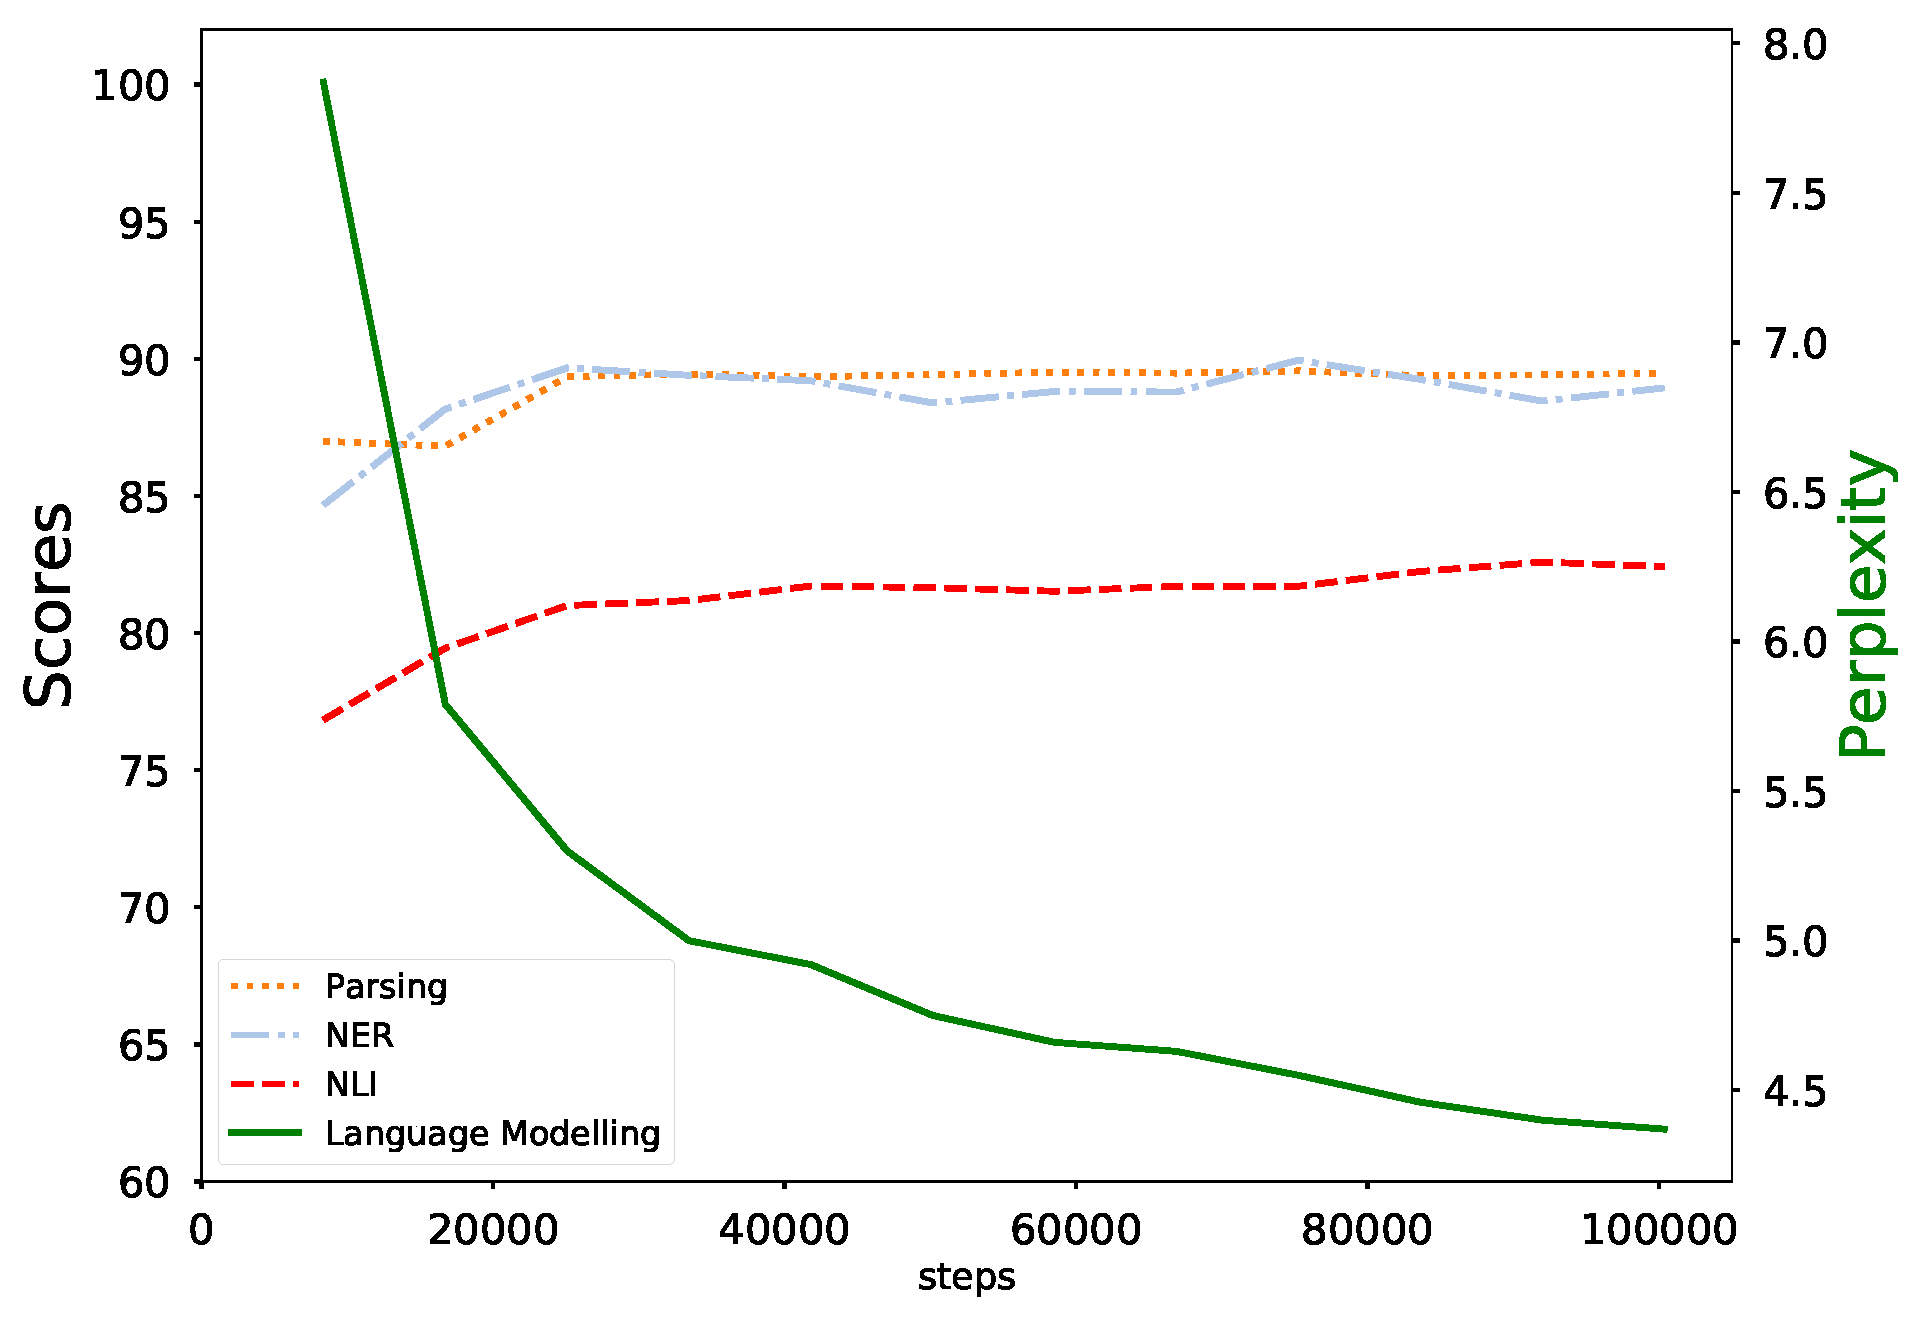
\includegraphics[width=\linewidth]{static/media/models/camembert/plot_steps_impact_4.pdf}
    \caption{Impact of number of pretraining steps on downstream performance for \camembert.}.
    \label{fig:n_steps_impact}
\end{figure}


Figure~\ref{fig:n_steps_impact} displays the evolution of downstream task performance with respect to the number of steps. % (1 step being 1 back-propagation update of a batch of 8192 sequences).
All scores in this section are averages from at least 4 runs with different random seeds. For POS tagging and dependency parsing, we also average the scores on the 4 treebanks.

We evaluate our model at every epoch (1 epoch equals 8360 steps). We report the masked language modelling perplexity along with downstream performances.
Figure~\ref{fig:n_steps_impact}, suggests that the more complex the task the more impactful the number of steps is. We observe an early plateau for dependency parsing and NER at around 22k steps, while for NLI, even if the marginal improvement with regard to pretraining steps becomes smaller, the performance is still slowly increasing at 100k steps.

In Table~\ref{tab:ablation}, we compare two models trained on \ccnet, one for 100k steps and the other for 500k steps to evaluate the influence of the total number of steps.
The model trained for 500k steps does not increase the scores much from just training for 100k steps in POS tagging and parsing.
The increase is slightly higher for XNLI (+0.84).


Those results suggest that low level syntactic representation are captured early in the language model training process while it needs more steps to extract complex semantic information as needed for NLI.
\chapter{FrELMo}
\chapter{D'Alembert}
\chapter{BERTrade}

\part{Downstream tasks}
\chapter{Parsing}
\chapter{POS Tagging}
\chapter{Named-Entity Recognition}
\chapter{Text Normalization}
\chapter{Document Structuration}

\part{Real World Application}
\chapter{BASNUM}
\chapter{Named-Entity Recognition corpora}


% This ensures that the subsequent sections are being included as root
% items in the bookmark structure of your PDF reader.
\bookmarksetup{startatroot}
\backmatter

\begingroup
\let\clearpage\relax
\glsaddall
\printglossary[type=\acronymtype]
\newpage
\printglossary
\endgroup

\printindex

% Entries for the entire Anthology, followed by custom entries
\bibliography{anthology, thesis}
\bibliographystyle{acl_natbib}

\end{document}
